\documentclass[a4paper, 12pt]{book}

\usepackage[utf8]{inputenc}
\usepackage{blindtext}
\usepackage{graphicx}
\usepackage{pgfplotstable}
\usepackage{booktabs}
\usepackage{filecontents}
\usepackage{longtable}
\usepackage{float}
\usepackage[T1]{fontenc}
\usepackage{tocloft}
\usepackage[backend=biber]{biblatex}
\addbibresource{references.bib}
\usepackage[skip=5pt plus1pt, indent=0pt]{parskip}

\usepackage[hidelinks]{hyperref}
\hypersetup{
    linktoc=all
    allcolors=black
}

\graphicspath{
  {./images/}
  {./troubleshooting/}
  {./sourdough-starter/}
  {./troubleshooting/crumb-structures/}
  {./history/}
  {./images/external/}
  {./baking/}
}

\interfootnotelinepenalty=10000

\advance\cftsecnumwidth 0.5em\relax
\advance\cftsubsecindent 0.5em\relax
\advance\cftsubsecnumwidth 0.5em\relax
\begin{document}

\begin{titlepage}
	\centering
  
\includegraphics[width=\textwidth]{cover-page}
  Version:
  \today
\end{titlepage}


\frontmatter

\tableofcontents

\chapter{Foreword}
Still need someone to write a foreword

\chapter{Preface}
If there is one food Germany is known for, it is probably bread.
There are thousands of varieties in Germany,
and making it has been an integral part of our culture.

My bread journey began during childhood. My mother, being a parent
of 3, would always use Saturdays to bake a delicious loaf for the family.
It was a white fluffy sandwich bread, and she made it within one to two hours using store-bought yeast.
Being a bit more experienced, I now realize it's
ideal to wait a little while before cutting into your bread, but back then,
we kids couldn't wait. Mom would cut for us a few slices straight from the oven, and we would
immediately proceed to pour butter or jam on each slice. Within minutes, 1kg of
flour would be consumed. Bread became an integral part of my weekly food.

I was lucky that my parents could afford a yearly ski trip to
Alto Adige in northern Italy. In the small town called Valdaora, we
would try new restaurants every year, yet always end up in our favorite
pizza place. The pizzas there were incredible. The dough
alone was so tasty that we would order just the bread with a
bit of olive oil and salt.

Of course, my question would always be, ``Mom, can we make this at home, too, please?''
So over the years, we became friends with the owners and would receive
more and more clues as how to make the perfect pizza dough. There
are no secret ingredients inside. It's just flour, water, salt, and a bit of yeast.
How can such a simple combination of ingredients create such an incredibly delicious
pizza dough? My parents, being creatures of habit, would return every year with us,
and every year, my interest would grow. At home, Mom and I attempted to replicate
the recipe. We tried baking on a stone and on a steel. We tried adding oil to the dough and herbs
to the pizza sauce. We fell into an endless cycle of experiments. However, we never managed
to get close to the experience we had while on vacation.

Some years passed, and I eventually began my studies in the small German city of Göttingen.
For the first time, I was faced with shopping for my own bread. It was never
on my mind to actually start baking it for myself. I would just buy 
a good loaf while shopping at the supermarket. My favorite variety
was a Schwarzbrot, Korn an Korn. It’s a very dark and hearty rye bread
with added berries and sunflower seeds. Being a little naive,
I'd never before examined the packaging of what I was buying. One day, that
changed.

I looked at the label and was shocked. The seemingly
healthy bread consisted of so many other things aside from flour and water.
The black color was not coming from the flour, but from caramelized sugar.
The packaging stated it was a sourdough bread, but then why was there additional yeast?
I thought that if it was really sourdough, it shouldn't require additional yeast, and I
soon realized that something was wrong with the bread I was buying.
I proceeded to check the other supermarket breads, only to discover that they, too,
contained ingredients I'd never heard of. That was the day I lost trust
in supermarket bread.

At home, I decided to research the proper way to make bread, and much to my surprise,
I learned that the recipes for making pizza and bread were actually quite similar, yet
there were also diffferences. For example, some recipes would call for fresh yeast, while
others would call for dry. Deep diving into various online forums and all their many
discussions, I became even more confused.

I tried using different flours and different brands, all in both organic and non-organic varieties.
I realized then that I knew nothing about making bread. Recipes would often contradict each other,
leaving me further confused. They seemed like little more than a collection of apparently random
steps to follow. The baking instructions and temperatures were all different, too.

Meanwhile, having completed my studies, I started work as an engineer.
We engineers are faced with many challenges. The compiler or runtime is
always screaming at you with errors, and it's your job to figure out how to fix them.
It can take hours, sometimes days just to fix a simple problem. If you want
to become a software engineer, you have to develop a certain ``never-give-up'' attitude.

Frequently when writing code, a set of pre-made routines are required. These routines have been
written by other engineers and can then be used to ship code faster.
This pre-written code is commonly known as {\it a framework}. In many cases,
these frameworks are not built by a single person but by engineers from all around the world,
each of whom can help by improving and changing the source code. Frameworks have made many successful
businesses possible.

In most cases, frameworks do exactly what they claim they do. However,
sometimes you are faced with issues you don't understand. In 99.95 percent
of all software bugs, the developer is the issue. Sometimes, however, the framework has a
bug. That is when the developer must dig deeper to see the what and the why behind what the
framework is doing. You will need to read other engineer's source code, and you will be forced
to understand {\it why} things are happening.

Being unhappy with what I was baking, my engineering mindset took over and I had
to do my own deep dive to understand what was going on. Much to my surprise, however,
none of the recipes I'd encountered would tell me {\it why} I should use amount X
of water and amount Y of flour, or {\it why} exactly I should use fresh yeast over dry yeast. Why
should I slap my dough while kneading it on the counter? Why is a standmixer
better than kneading by hand?  Why should I let the dough sit for this long?
Why is steaming the dough during baking important? Do I really need to
get myself an expensive dutch oven to bake bread?

The problem compounded when I started reading about sourdough. It all sounded like black
magic. Why were some sourdoughs made from fruits, while others were made from flour?
Why should one recipe use wheat while another used rye or spelt? How often should the
sourdough be fed? The questions I had then could have filled 20 pages. I was confused,
but became even more determined to learn how decent bread should be made at home.

The feedback I received from friends helped me to improve with each
iteration of homemade bread. Compared to coding, where you sometimes have to wait months
for this feedback, bread making is much more direct. Plus, you can eat your successes
(and failures!) And, much to my surprise, even those failures started tasting better than
most store-bought breads. Eating a homemade bread that takes you hours to make allows you
to develop a different relationship with your food, and baking bread from scratch with my
bare hands was a welcome change after hours of working on the computer.

I continued learning about the process of fermentation and various techniques of bread making.
I approached the topic of sourdough in a manner similar to software, and after years of
researching and documenting my progress, I decided it was time to share that progress with the
world.

When working on open source projects, it is important to see their history and how the source
code changes over time. This way, you can easily jump back to previous versions. This was
the perfect tool for documenting my recipes, because they, too, would change with each
subsequent iteration. Much to my surprise, my open source work on sourdough was appreciated
by other engineers, and the project became popular on the website GitHub, originally built to
share open source software.

Now, when baking great bread, you also need to learn certain techniques. I figured it would be
easier to share these techniques in video form. Thus, my YouTube channel was born. I chose
the name {\it The Bread Code} to capture my engineering-oriented approach to bread. It took some
time to get right, but after choosing more engaging thumbnails and titles for
the videos I made, the channel started gaining viewers.

Now, three years later, I dedicate two days each week to follow my bread baking passion, while
the other three days I continue to work as a software engineer, writing code on a day-to-day
basis.

My bread days fill me with both joy and passion. To me, there is nothing better than seeing
how many people have made amazing bread thanks to my tips and explanations. The community has
continued to grow, spawning many interesting discussions and ideas surrounding the topic of
bread making. There is always something new to learn, and I feel that even now I am just barely
scratching the surface with what I know and teach. Would you ever have imagined that fruit
flies are like bees and are part of the wild yeast's success story? I made a video where
I tried to cultivate wild yeast spores coming from fruit flies in order
to bake bread. It worked; the bread turned out amazing and even tasted good! These kinds of
experiments spark my natural interest. Conducting them and seeing how other people share in my
interest makes me incredibly happy.

The problem with running a YouTube channel is that all the information
you see is filtered and then provided to you through an algorithm. I am concerned
with how algorithms are shaping modern information, because they tend to
put users into certain categories where they will then only see news related to
those same fixed categories. A key metric determining visibility of your channel is how many
people have clicked on a video after it's been shown, and the content you create
is not even shown to every subscriber of your channel. If the algorithm determines the video
is not engaging enough, your content starts to decay in YouTube's nirvana. Even if your video
goes viral, the algorithm will stop showing it once engagement rates with new users goes down,
and older videos fade over time as the decay punishment factor increases. I know, because
I have developed similar algorithms myself as a software engineer.

I've since decided to take some time off from the algorithm cycle to work on something more
long term and meaningful. My mission has always been to share my knowledge with as many people
in the world as possible. That's also why my content has been provided in English rather than
German. After discussing with members of the community, I figured that writing a book could
help me achieve that goal. Most of the books that exist today are collections of recipes. My
idea, however, is to provide you with a deeper foundation of knowledge that you can use to
follow other recipes.

In software terms, this would be a {\it bread framework}.

It is my goal for this book to help everyone facing issues with flour, fermentation, baking,
and more. It should provide a detailed understanding as to why certain steps are necessary
and how to adapt then when things go wrong while making bread.

It is my desire for this knowledge to be accessible to everyone around the world, regardless
of budget, and as such, do not want to charge for the book. That's why I've decided to make
it open source and have asked the community to support my work financially via my ko-fi page
(https://ko-fi.com/thebreadcode). The community's feedback has been amazing so far, and
I've already raised much more money than initially expected.

The first version of the book will only be available digitally---this way, everyone can read
it---though there might also be a hardcover version in the future, depending on how well received
and appreciated it is by bakers around the world. The hardcover version will, of course, cost a
bit of money, but the digital version will remain free.

In this book, I will try to be as scientific as possible. I in no way claim, however, that
it will itself be a work of science. I have conducted several experiments that I will write
about here, but to truly call this science, you would probably need to repeat the same experiment
a thousand times in a lab environment, which I have not done. I will do my best, however, to provide
scientific references where possible and to clearly distinguish between facts and personal opinion.

I hope you have fun reading this and that you learn more about the fascinating world of bread
making, and it is my sincere wish that this work provides you with the solid toolchain that I wish
I'd had access to when starting my own journey with bread.

Thank you.
Hendrik

\chapter{Acknowledgements}
This book would not have been possible without your help.

With all your donations I have been able to take time off from my job and
focus on this project.

Furthermore many of you have contributed and improved the
instructions, fixed spelling mistakes and/or provided
feedback on the content. Each of you has made this book
better.

By providing this book free of charge,
we can enable more people around the world to bake delicious sourdough
bread at home.

Thank you very much for your support!\\

\begin{filecontents}{supporters.csv}
  \end{filecontents}

  {\large Big shout-out to all the initial supporters:}

  \pgfplotstableset{
  begin table=\begin{longtable},
  end table=\end{longtable},
  }

  \pgfplotstabletypeset[col sep=comma,
  header=true,
  columns={Name},
  columns/Name/.style={column type=l,string type},
  every head row/.style={before row=\toprule, after row=\midrule\endhead},
  every last row/.style={after row=\bottomrule}
  ]{supporters.csv}


\mainmatter

\chapter{The history of sourdough}
Sourdough has been made since ancient times. The exact origins
of fermented bread are however unknown. One of the most ancient
preserved sourdough bread has been excavated in Switzerland.
However, based on recent research, some scientists speculate
that sourdough bread has already been made in 12000 BC in ancient
Jordan \cite{jordan+bread}.

\begin{figure}[h]
  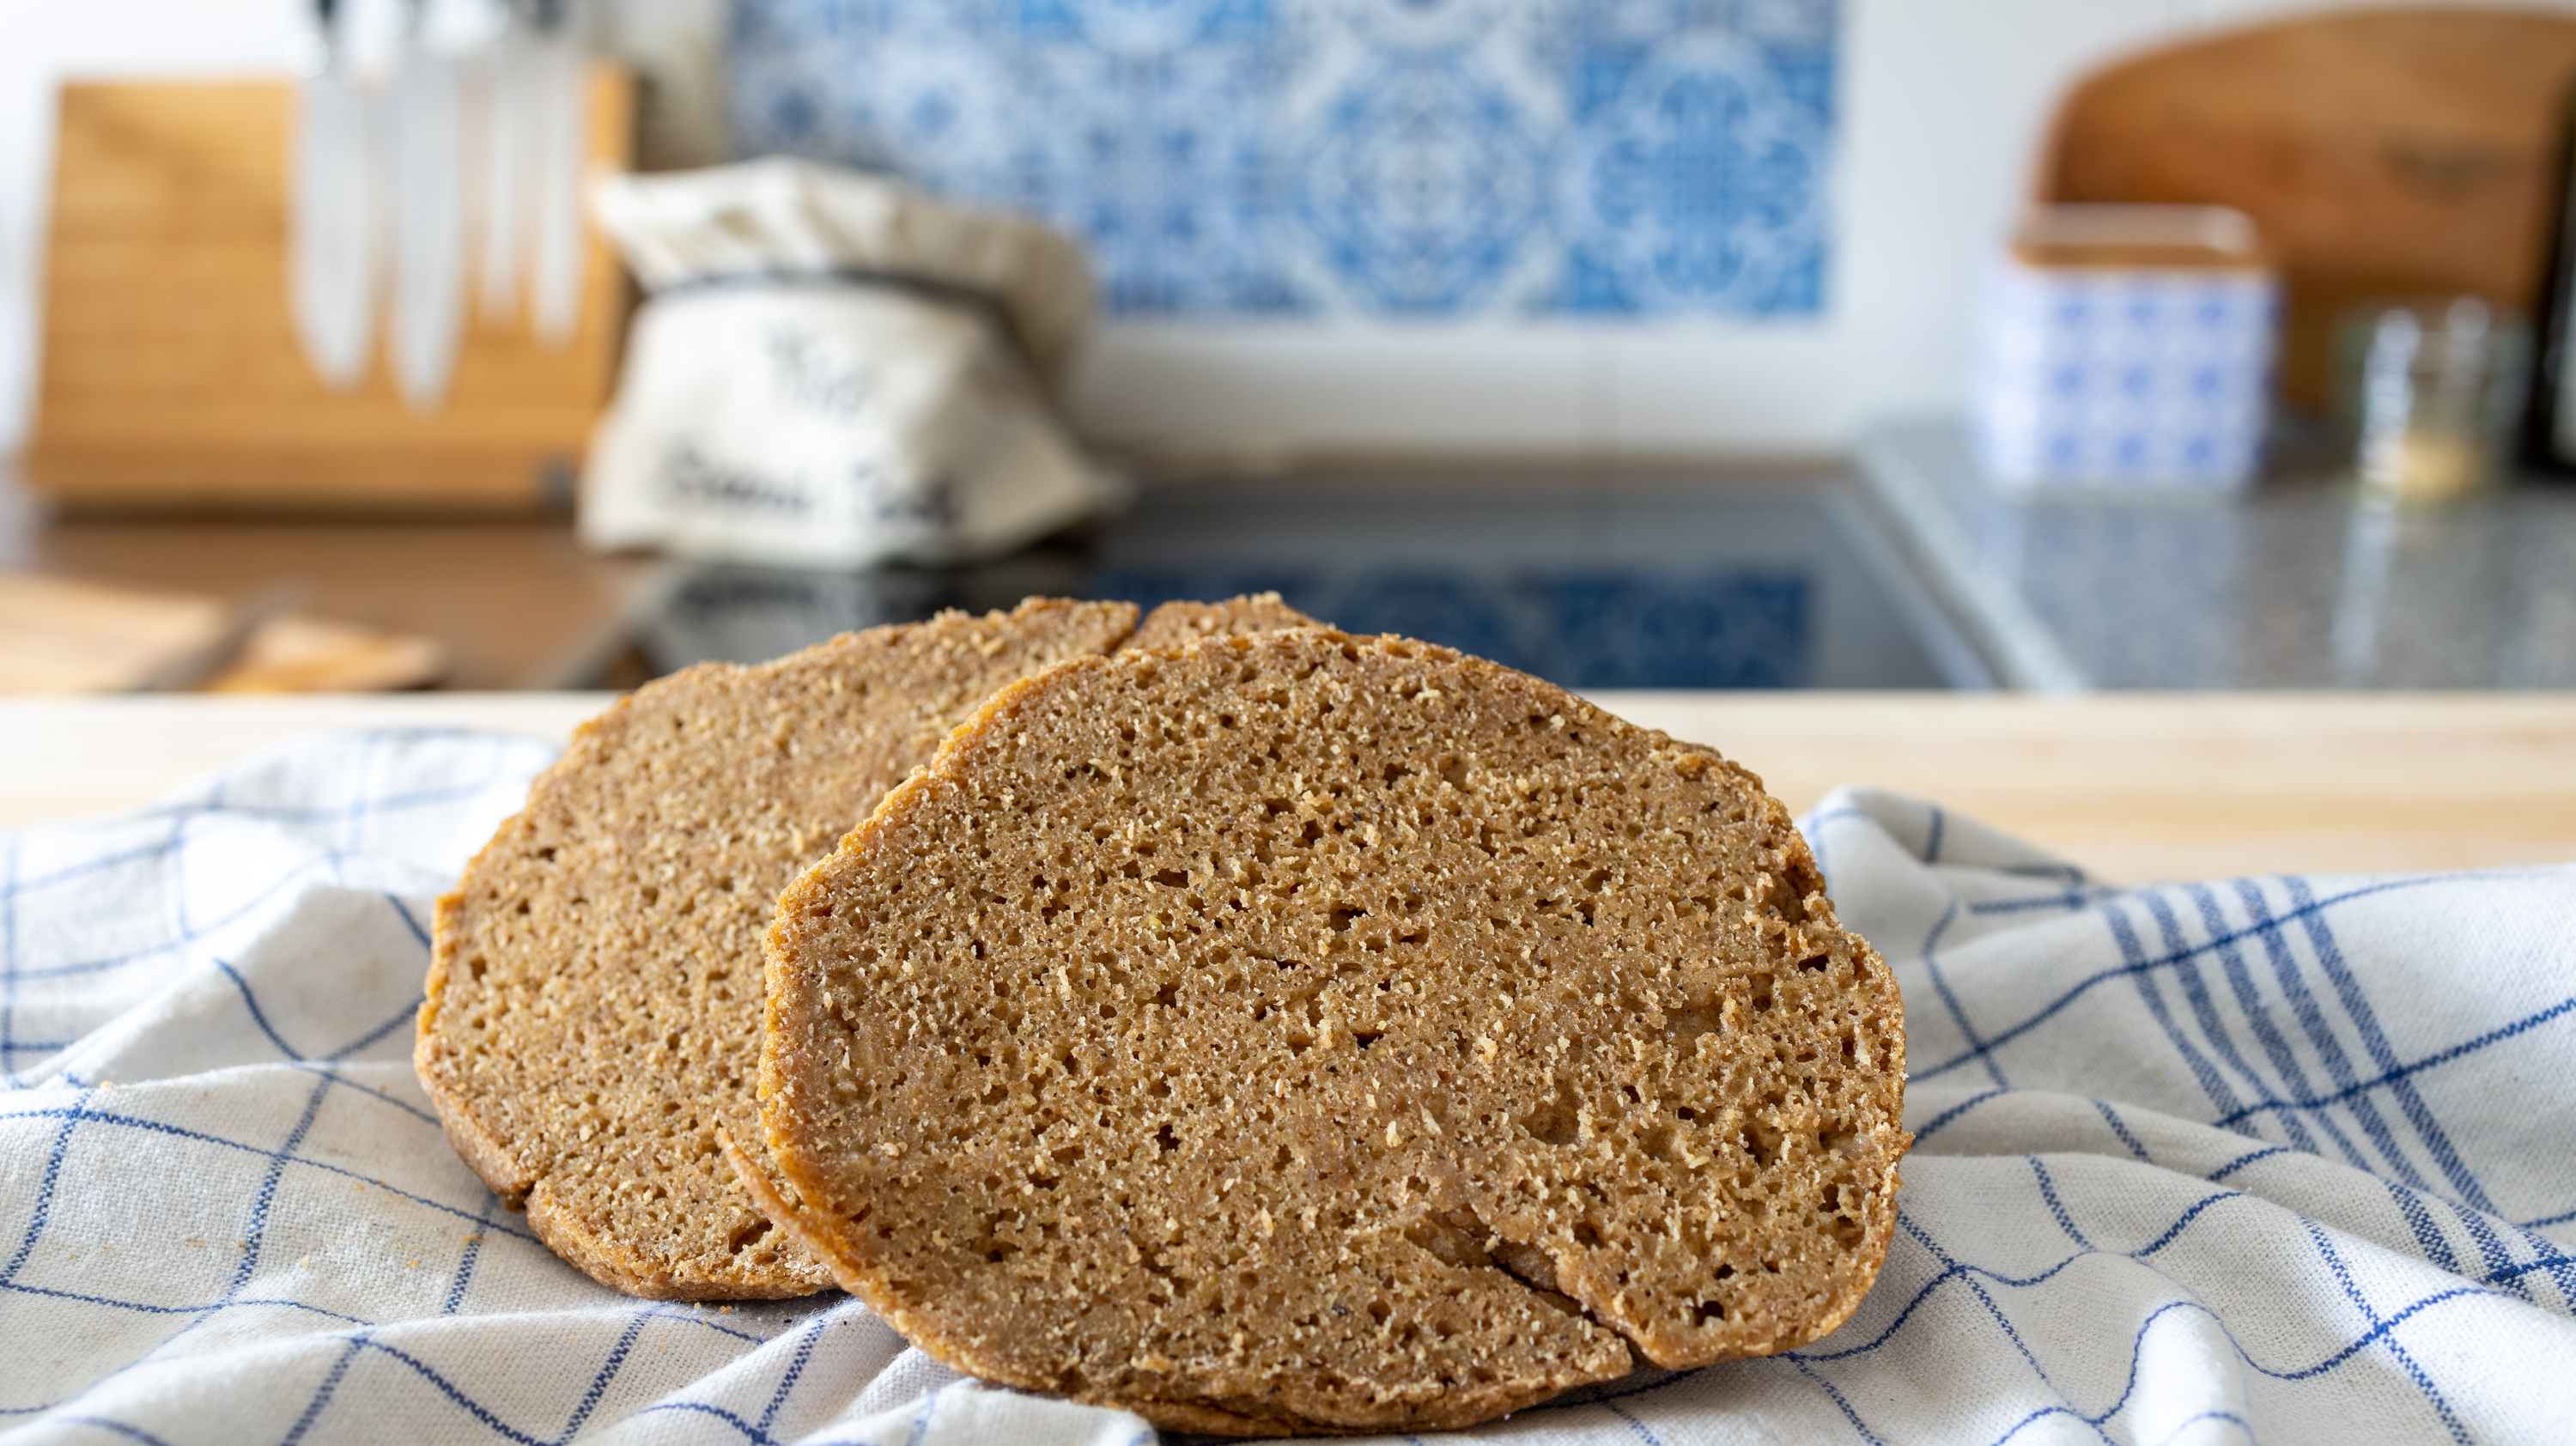
\includegraphics[width=\textwidth]{einkorn-crumb}
  \caption{An ancient Einkorn flatbread. Note the denser crumb structure.}
  \label{einkorn-crumb}
\end{figure}

Another popular story is that a lady in Egypt was making
a bread dough close to the Nile river. The lady forgot the
dough and returned a few days later. She would notice that
the dough had increased in size and smelled funky. She decided
to bake the dough anyways. She was rewarded with a much
lighter softer better tasting bread dough. From that day
on she continued to make bread this way.

Little did the people back then know that tiny microorganisms
were the reason they made better bread. It is not clear when
people started using a bit of the dough from the previous
day for the next batch of dough. But by doing so sourdough
bread making was born. Wild yeast on the flour and in the air
plus bacteria start to decompose the flour-water mixture, also
known as your dough. The yeast makes the dough fluffy and
the bacteria primarily creates acidity. Both the different
microorganisms work in a symbiotic relationship. Humans
appreciated the enhanced airy structure and slight acidity
of the dough. Furthermore, the shelf life of such bread
was extended due to the increased acidity. 

Quickly similar processes were discovered when brewing beer
or making wine. A small tiny batch of the previous production
would be used for the next production. In this way, humans created
modern bread yeasts, wine yeasts, and beer yeasts. Only in 1680
the scientist Anton van Leeuwenhoek first microscoped yeast
microorganisms. Over time with each batch, the yeasts and bacteria
would become better at consuming whatever they were thrown at.
By feeding your sourdough starter you are selectively breeding
microorganisms that are good at eating your flour. With
each iteration, your sourdough knows how to better ferment the flour
at hand. This is also the reason why more mature sourdough starters sometimes
tend to leaven doughs faster (source needed). It is crazy if you
think about it. People have been using this process despite not
knowing what was actually going on for thousands of years! The
sourdough in itself is a symbiotic relationship. But the sourdough
also adapted to humans and formed a symbiotic relationship with us.
For food and water, we are rewarded with delicious bread. In exchange,
we shelter and protect the sourdough. Spores from the starter
are spread through aerial contamination or insects like fruit flies.
This allows the sourdough starter to spread its spores even
further all around the world. 

Brewers would start to experiment with utilizing the muddy leftovers
of the beer fermentation to start making doughs. They would notice
that the resulting bread doughs were becoming fluffy and compared
to the sourdough process would lack the acidity in the final product.
A popular example is shown in a report from 1875. Eben Norton Horsford
would write about the famous "Kaiser Semmeln" (Emperor's bread rolls).
These are essentially bread rolls made with brewer's yeast instead
of the sourdough leavening agent. As the process is more expensive
bread rolls like these were ultimately consumed by the noble people
in Vienna \cite{vienna+breadrolls}.

\begin{figure}[h]
  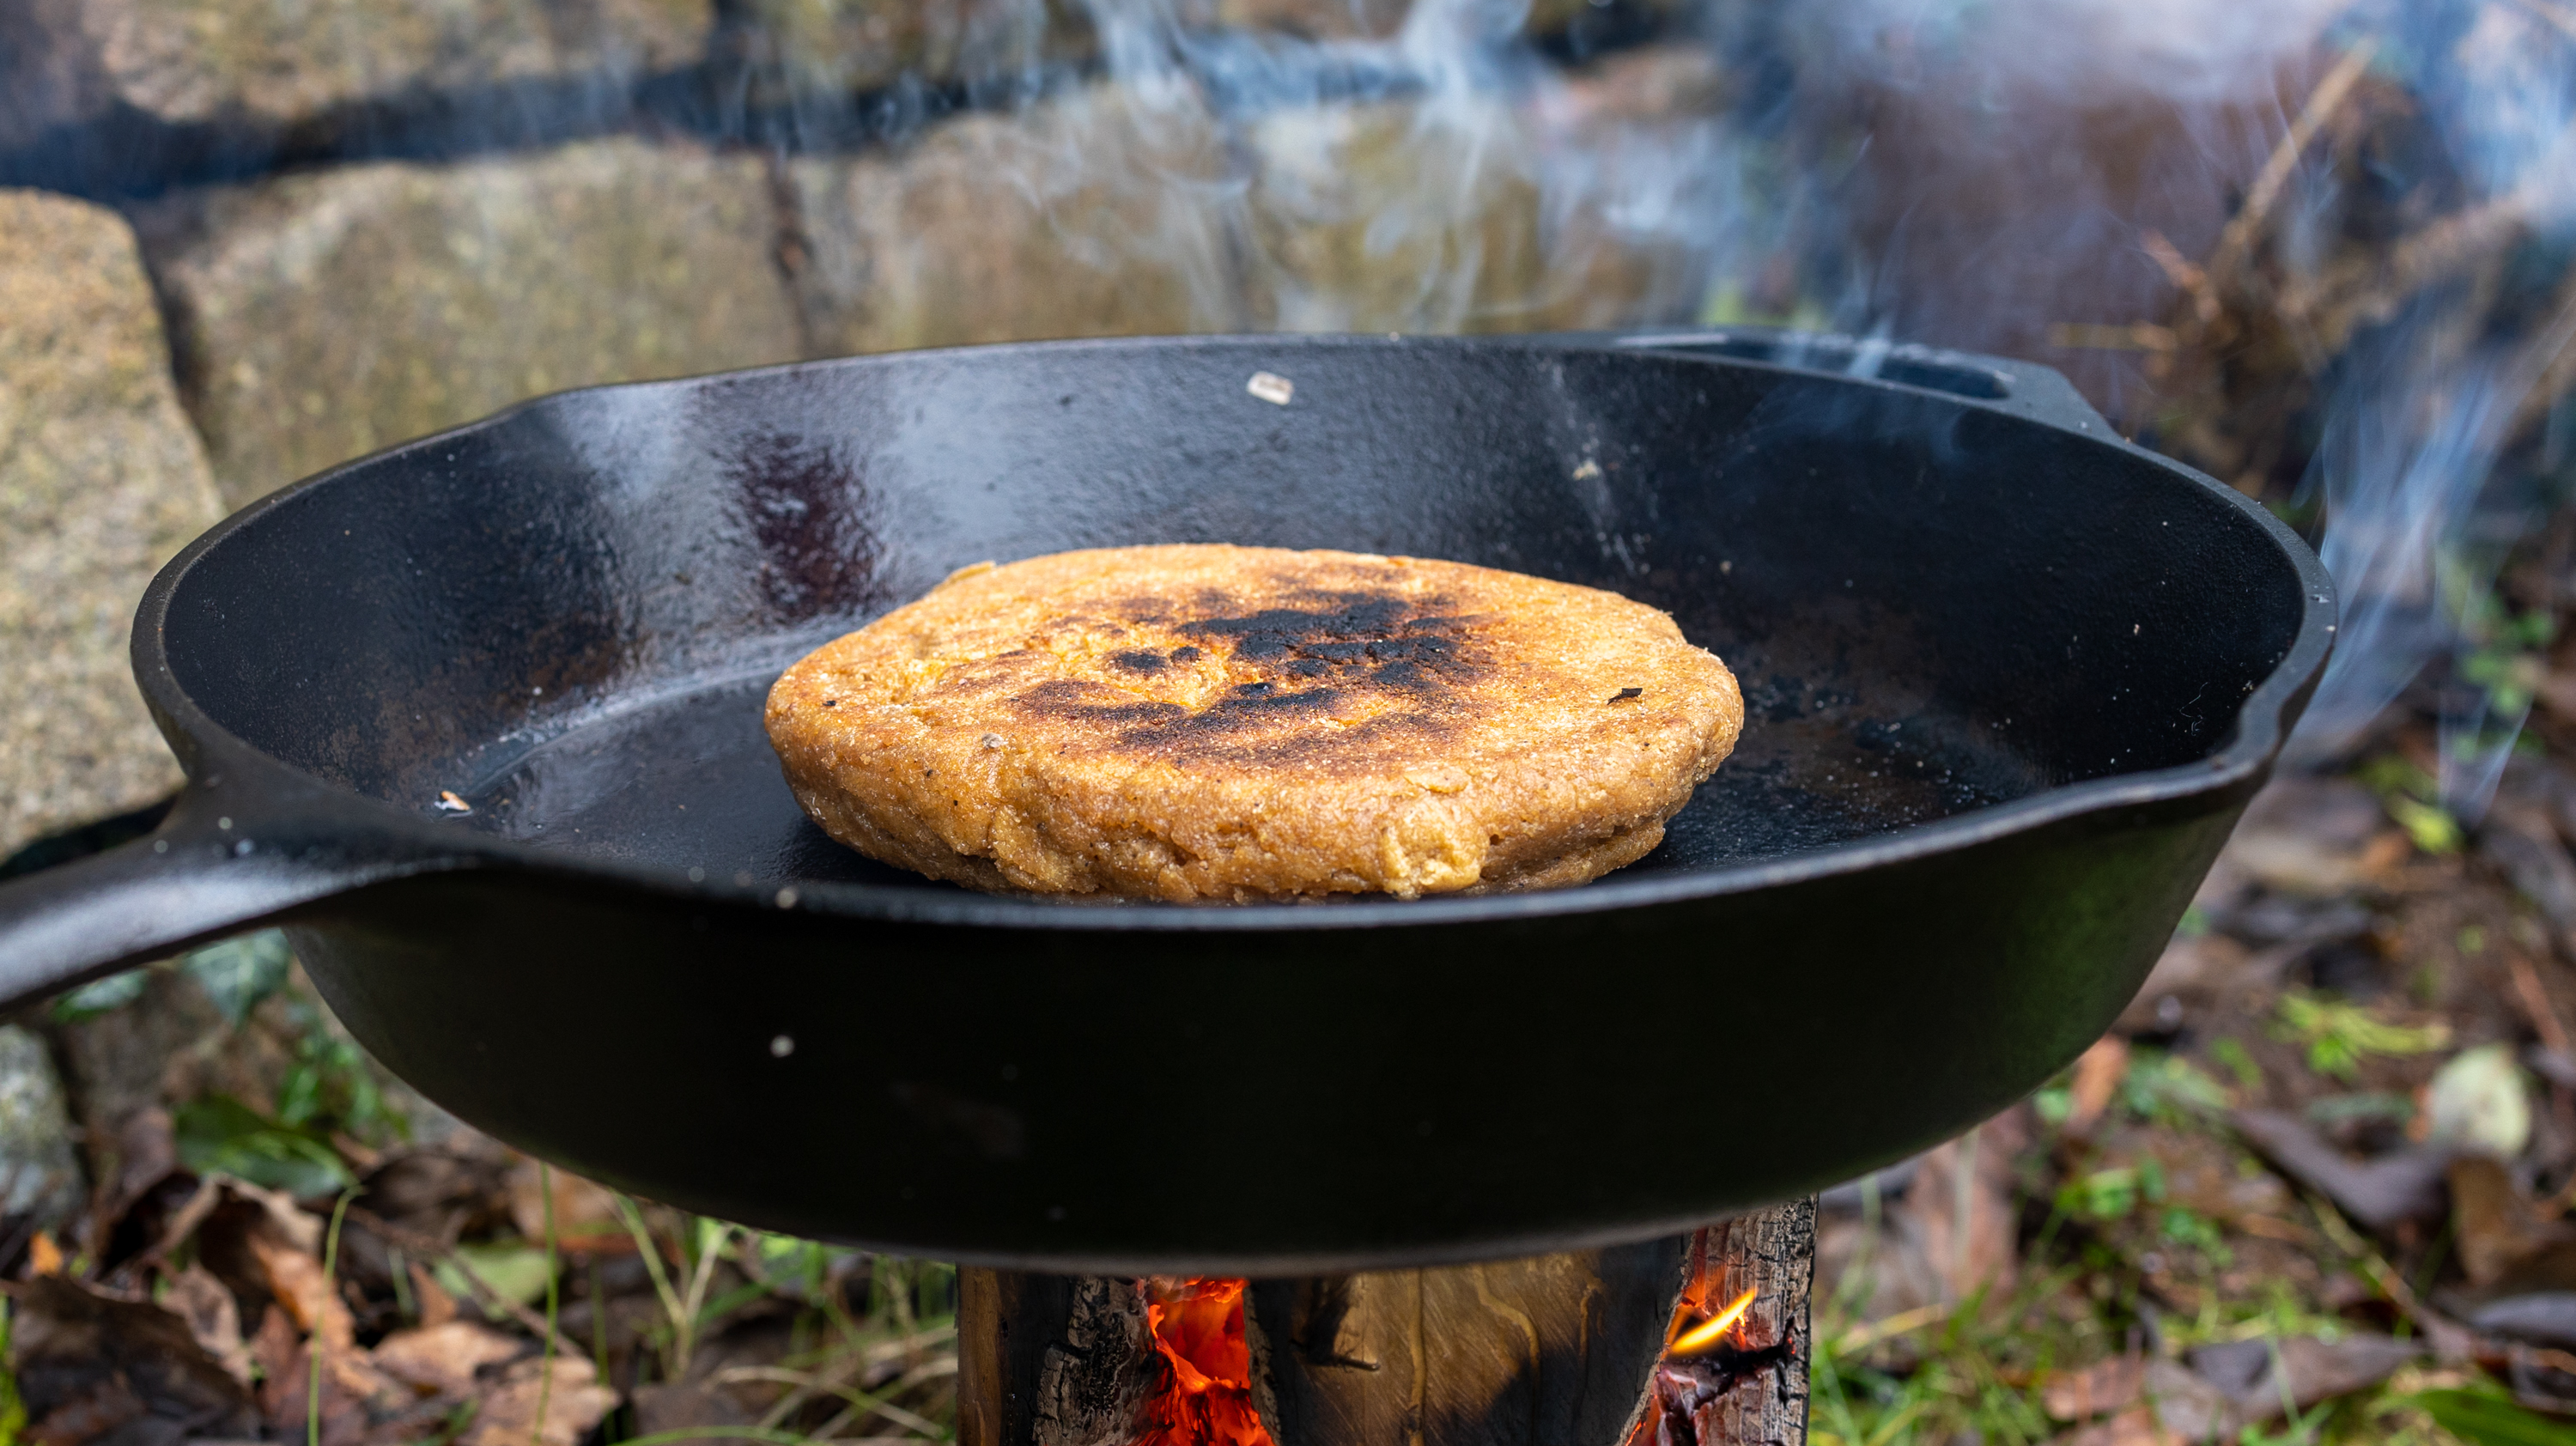
\includegraphics[width=\textwidth]{sourdough-stove}
  \caption{A bread made over the stove without an oven}
  \label{sourdough-stove}
\end{figure}

Only in 1857, the French microbiologist Louis Pasteur discovered
the process of alcoholic fermentation. He would prove that
yeast microorganisms are the reason for alcoholic fermentation
and not other chemical catalysts. What would then start is
what I describe as the 150 lost years of bread making. In 1879
the first machines and centrifuges were developed to centrifuge
pure yeast. This yeast would be extracted from batches of sourdough.
The pure yeast would prove to be excellent and turbocharged
at leavening bread doughs. What would previously take 10 hours
to leaven a bread dough could now be done within 1 hour.
The process became much more efficient. During world war II
the first packaged dry yeast was developed. This would ultimately
allow bakeries and home bakers to make bread way faster.
Thanks to pure yeast, building bread making machines was
possible. Provided you have the same temperature your yeast
would always ferment exactly the same way. As fermentation
times sped up the taste of the final bread would deteriorate.
The sprouting process induced by certain enzymes is essential
to developing a fluffier texture and better tasting crust. This
can't be indefinitely sped up. Soon bakeries would start
to introduce additional enzymes to achieve similar properties
to sourdough bread in yeast-based doughs. Sourdough almost
completely vanished from the surface. Only a handful
of true nerds would continue making bread with sourdough.
Suddenly people started to talk more often about celiac disease
and the role of gluten. The disease isn't old, it has first
been described in 250 AD \cite{coeliac+disease}. People
would note how modern bread has much more gluten compared
to ancient bread. The bread in ancient times probably was way flatter.
The grains over time have been bread more and more towards containing a higher
amount of gluten. Gluten is a protein that gives modern
bread its typical soft fluffy crumb structure. The
gluten proteins bind together once activated with water.
Throughout the course of the fermentation, CO2 is trapped
in this protein matrix. The tiny created chambers expand
during the baking process. As the dough gelatinizes while
being heated the structure is fortified. This makes the bread appear
soft and fluffy when tasting it. Similar to drinking
raw cow milk your immune system might react to
the consumed proteins. There is gluten intolerance
and celiac disease. When people say they don't handle
gluten well it's mostly a gluten intolerance they describe.
Some people describe similar issues when consuming
too much lactose. If you eat a long-fermented cheese
however most of the lactose has been fermented by
the tiny microorganisms. People would investigate and
note how sourdough bread can typically be handled better
compared to plain fast made factory bread. The
reason for this is that enzymes take time to work the dough.
Gluten is a storage protein of flour. Once
sprouting is activated by adding water, the protease
enzyme starts to convert the gluten into tinier amino acids
that are required for sprouting. Over time you are effectively
losing gluten as it's naturally broken down. Furthermore,
traditionally lactic acid bacteria would start to decompose
the flour-water mix. Almost everything is recycled in nature.
Part of their diet is to consume the proteins in the dough.
Modern bread is faster and no longer has lactic acid bacteria.
Both factors together mean that you are consuming products
with a much higher gluten value compared to ancient times
when natural fermentation was used \cite{raffaella+di+cagno}.

During the California Gold Rush, French bakers brought the sourdough
culture to Northern America. A popular bread became the
San Francisco sourdough. It's characterized by its unique
tang (which was previously common for every bread). It
however remained more of a niche food. What really expedited
the comeback of sourdough was the 2020 COVID-19 pandemic.
Flour and yeast became scarce in the supermarkets. While
flour returned yeast couldn't be found. People started
to look for alternatives and rediscovered the ancient
way of making sourdough bread. Soon many realized
that making sourdough bread is more complex than modern
yeast-based bread. You need to maintain a sourdough starter
and have it in ideal shape to properly ferment your dough.
Furthermore compared to a yeast-based dough you can't just
punch the dough down and let the fermentation continue.
You can overferment your dough, resulting in a sticky
dough mess. This complexity lead to many bakers looking
for help and many thriving communities formed around
the topic of homemade bread.

When interviewing Karl de Smedt (owner of the Sourdough
Library) he said something that changed my way of thinking
about bread: "The future of
modern bread is in the past \cite{interview+karl+de+smedt}."


\chapter{How sourdough works}
In this chapter, we will cover the basics of how sourdough ferments.
First, we will look at the enzymatic reactions that take place
in your flour the moment you add water, triggering the fermentation
process. Then, in order to understand this process better, we will
learn more about the yeast and bacterial microorganisms involved.

\begin{figure}[!htb]
  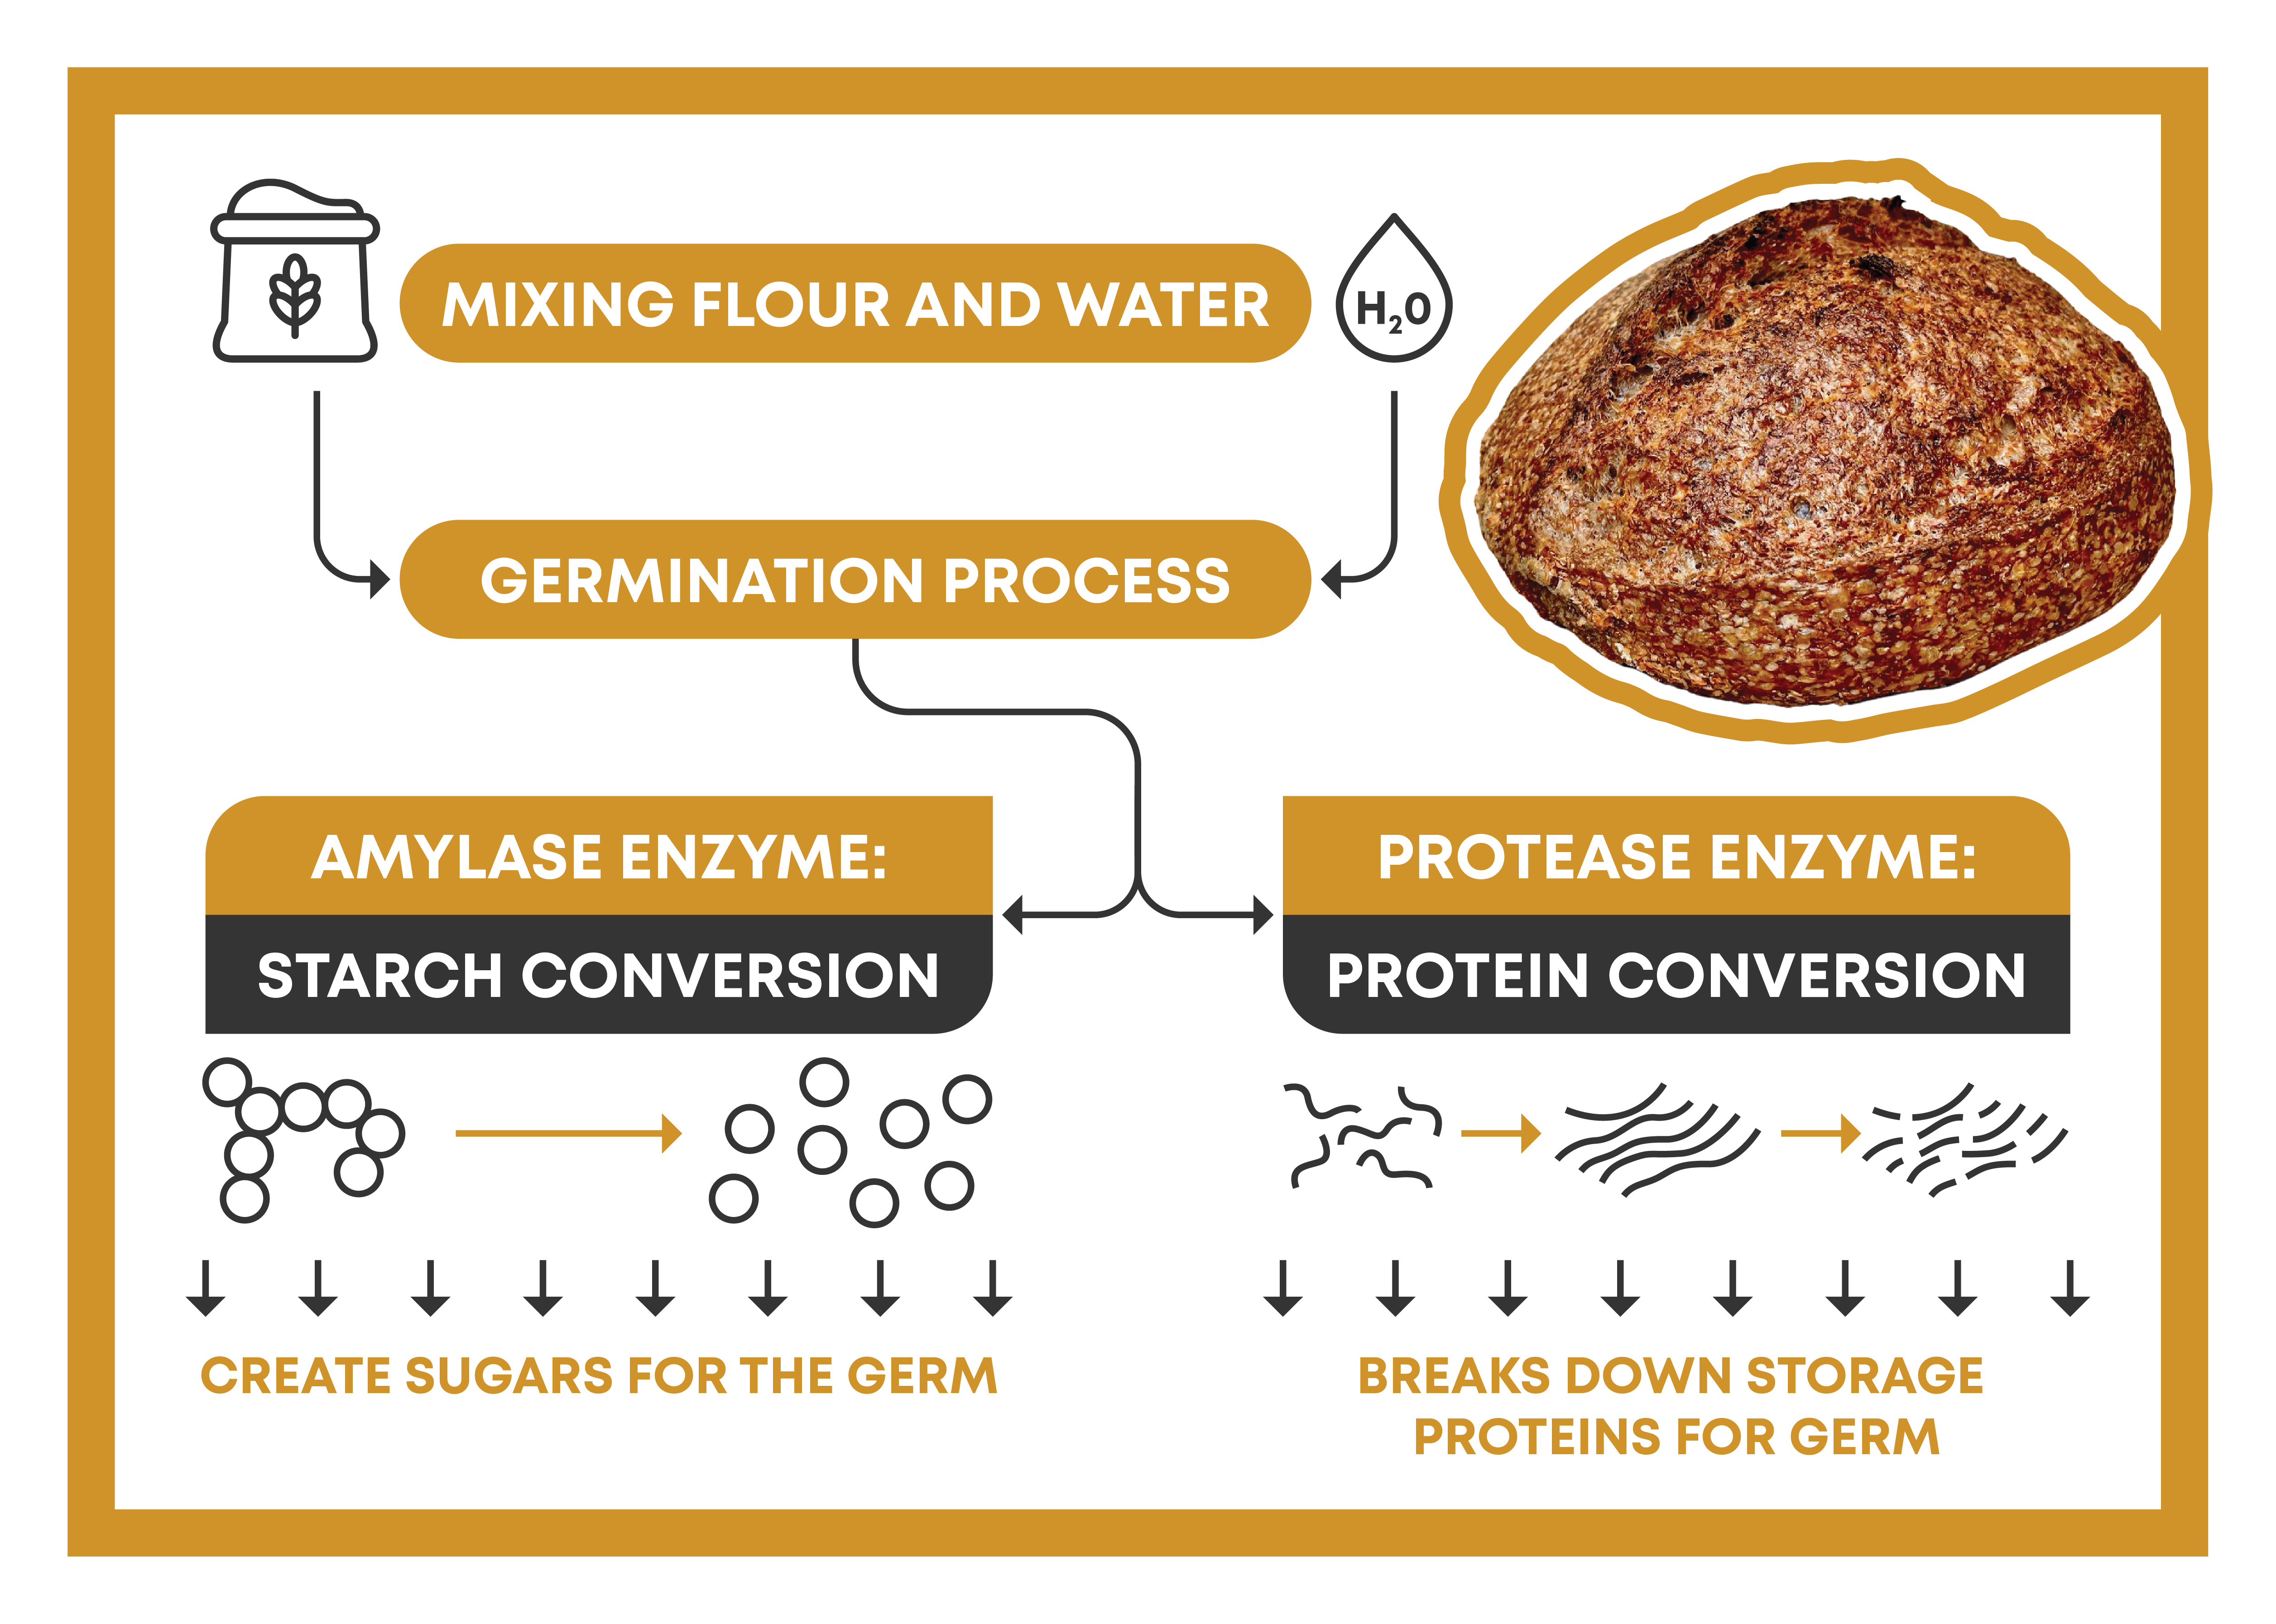
\includegraphics[width=\textwidth]{infographic-enzymes}
  \caption{How amylases and proteases interact with flour}
  \label{infographic-enzymes}
\end{figure}

\section{Enzymatic reactions}

To understand the many enzymatic reactions that take place when flour
and water are mixed, we must first understand seeds and their role in
the lifecycle of wheat and other grains.

Seeds are the primary means by which many plants, including wheat,
reproduce. Each seed contains the embryo of another plant, and must
therefore contain all the nutrients that new plant requires to grow.

When the seed is dry, it is in hibernation mode and can sometimes be
stored for several years. The moment it comes into contact with water,
however, it begins to sprout. The seed turns into a germ, requiring the
stored nutrients to be converted into something the plant can use while
it grows. The catalyst that makes the associated reactions possible is water.

The seed typically contains the first prototypical leaves of the plant,
and it can put down roots using the stored nutrients inside. Once those leaves
break through the soil and come into contact with the sunlight above, they
begin to photosynthesize. This process is the plant's engine, and with the
energy photosynthesis produces, the plant can continue to grow more roots,
enabling it to access additional nutrients from the soil. These additional
nutrients allow the plant to grow more leaves, increasing its photosynthetic
activity so that it can thrive in its new environment.

Of course, a ground flour can no longer sprout. But the enzymes that
trigger this process are still present. That's why it's important not to
mill grains at too high a temperature, as doing so could damage some of
these enzymes.

Normally, the grain seed shields the germ against pathogens. However, as the
grain is ground into flour, the contents of the seed are exposed. This is ideal
for our sourdough microorganisms.

Neither the yeast nor the bacteria can prepare their own food. However, as
the enzymes are activated, the food they need becomes available, allowing them
to feed and multiply.

The two main enzymes involved in this process are \textit{amylase} and
\textit{protease}. For reasons that will soon be made clear, they are of the
utmost importance to the home baker, and their role in the making of sourdough
is a key puzzle piece to making better-tasting bread.

\subsection{Amylase}

Sometimes, when you chew on a potato or a piece of bread for a long period
of time, you'll perceive a sweet flavor on your tongue. That's because your
salivary glands produce amylase. Amylase breaks down complex starch molecules
into easily-digestible sugars. Your body uses amylase to start the digestive
process. The germ works similarly by using the same enzyme. The amylase
is used to create sugars out of the starch to then produce more plant matter.

Normally,
the microorganisms on the surface of the grain can't consume the freed maltose
molecules, which remain hidden inside the germ. But as we grind the flour, a
feeding frenzy takes place. Generally, the warmer the temperature, the faster
this reaction occurs. That's why a long fermentation is key to making great
bread. It takes time for the amylase to break down most of the starch into
simple sugars, which are not only consumed by the yeast but are also essential
to the \textit{Maillard reaction}, responsible for enhanced browning during the
baking process.

If you're a hobby brewer, you'll know that it's important to keep your beer at
certain temperatures to allow the different amylases to convert the contained
starches into sugar \cite{beer+amylase}. This process is so important that
there's a frequently used test to determine whether or not all the starches
have been converted.

This test, called the \textit{Iodine Starch Test}, involves mixing iodine into
a sample of your brew and checking the color. If it's blue or black, you know
you still have unconverted starches. I wonder if such a test would also work
for bread dough?

Industrial bakers that add especially active yeast to produce bread in a short
period of time face a similar issue. Their approach is to add malted flour to
the dough. The malted flour contains many enzymes and thus speeds up the
fermentation process. The next time you're at the supermarket, check the
packaging of the bread you buy. If you find {\it malt} in the list of
ingredients, chances are this strategy was used.

Note that there are actually two categories of malt. One is {\it enzymatically
active malt}, which has not been heated to above 70°C, where the amylases begin
to degrade. The other is {\it inactive malt}, which has been heated to higher
temperatures and thus has no impact on your flour.

\subsection{Protease}

Just as amylase breaks starches down into simple sugars, protease breaks
complex proteins down into simpler proteins and amino acids. Because wheat
contains gluten, a protein that's essential to the structure of bread,
protease necessarily plays a crucial role in the baking of sourdough.

Since the grain seeds require smaller amino acids to build roots and other
plant materials, the gluten in those seeds will begin to break down the moment
they sprout, and since adding water to flour activates those same enzymes,
the same process occurs in bread dough.

If you've ever tried to make a wheat-based dough and kept it at room
temperature for several days, you'll have discovered for yourself that the
gluten network breaks down so that the dough can no longer hold together. Once
this happens, the dough easily tears, holds no structure, and is no
longer suitable for baking bread.

This happened to me once when I tried to make sourdough directly from a dried
starter. At three to four days, the fermentation speed was so slow that the
gluten network broke down. The root cause for this issue was protease.

By adding water to your dough, you activate the protease, and this gets to work
in readying amino acids for the germ.

Here's another interesting experiment you can try to better visualize the
importance of protease: Make a fast-proofing dough using a large quantity
of active dry yeast. In one to two hours, your dough should have leavened and
increased in size. Bake it, then examine the crumb structure. You should see
that it's quite dense and nowhere near as fluffy as it could have been. That's
because the protease enzyme wasn't given enough time to do its job.

At the start, while kneading, a dough becomes elastic and holds together very
well. As that dough ferments, however, it becomes more loose and extensible
\cite{protease+enzyme+bread}. This is because some of the gluten bonds have
been broken down naturally by the protease through a process known as
\textit{proteolysis}. This is what makes it easier for the yeast to inflate the
dough, and it's why a long fermentation process is critical when you want to
achieve a fluffy, open crumb with your sourdough bread.

Aside from using great ingredients, the slow fermentation process is one of the
main reasons Neapolitan pizza tastes so great: because the protease creates an
extensible, easy-to-inflate dough, a soft and airy edge is achieved.

Because the fermentation process typically takes longer than eight hours, a
flour with a higher gluten content should be used. This gives the dough more
time to be broken down by the protease without negatively affecting its
elasticity. If you were to use a weaker flour, you might end up with a dough
that's broken down so much that it tears during stretching, making it
impossible, for example, to shape it into a pizza pie.

Traditionally, pizza has been made with sourdough, but in modern times it is
made with active dry yeast, as the dough stays good for a longer period of time
and is much easier to handle on a commercial scale. If you were to use
sourdough, you might have a window of thirty to ninety minutes before the dough
begins to deteriorate, both because of the protease acting for a longer period
of time and the byproducts of bacteria, which we'll discuss in more detail later
in this chapter.

\subsection{Improving enzymatic activity}

As explained previously, malt is a common trick used to speed up enzymatic
activity. Personally, however, I prefer to avoid malt and instead use a
trick I learned while making whole-wheat breads.

When I first started making whole-wheat bread, I could never achieve the
crust, crumb, or texture I desired no matter what I tried. Instead, my dough
tended to overferment rather quickly. When using a white flour with a similar
gluten content, however, my bread always turned out great.

At the time, I utilized an extended autolyse, which is just a fancy word for
mixing flour and water in advance and then letting the mixture sit. Most
recipes call for it as the process gives the dough an enzymatic head start, and
in general it's a great idea. However, as an equally effective alternative,
you could simply reduce the amount of leavening agent used (in the case of
sourdough, this would be your starter). This would allow the same biochemical
reactions to occur at roughly the same rate without requiring you to mix your
dough several times. My whole wheat game improved dramatically after I stopped
autolysing my doughs.

Now that I've had time to think about it, the result I observed makes sense.
In nature, the outer parts of the seed come into contact with water first, and
only after penetrating this barrier would the water slowly find its way to the
center of the grain. The seed needs to sprout first to outcompete other nearby
seeds, requiring water to enter quickly. Yet the seed must also defend itself
against animals and potentially hazardous bacteria and fungi, requiring some
barrier to protect the embryo inside. A way for the plant to achieve both goals
would be for most of the enzymes to exist in the outer parts of the hull. As a
result, they are activated first (source needed). Therefore, by just adding a
little bit of whole flour to your dough, you should be able to significantly
improve the enzymatic activity of your dough. That's why, for plain white flour
doughs, I usually add 10\textendash20\% whole-wheat flour.

\begin{figure}
  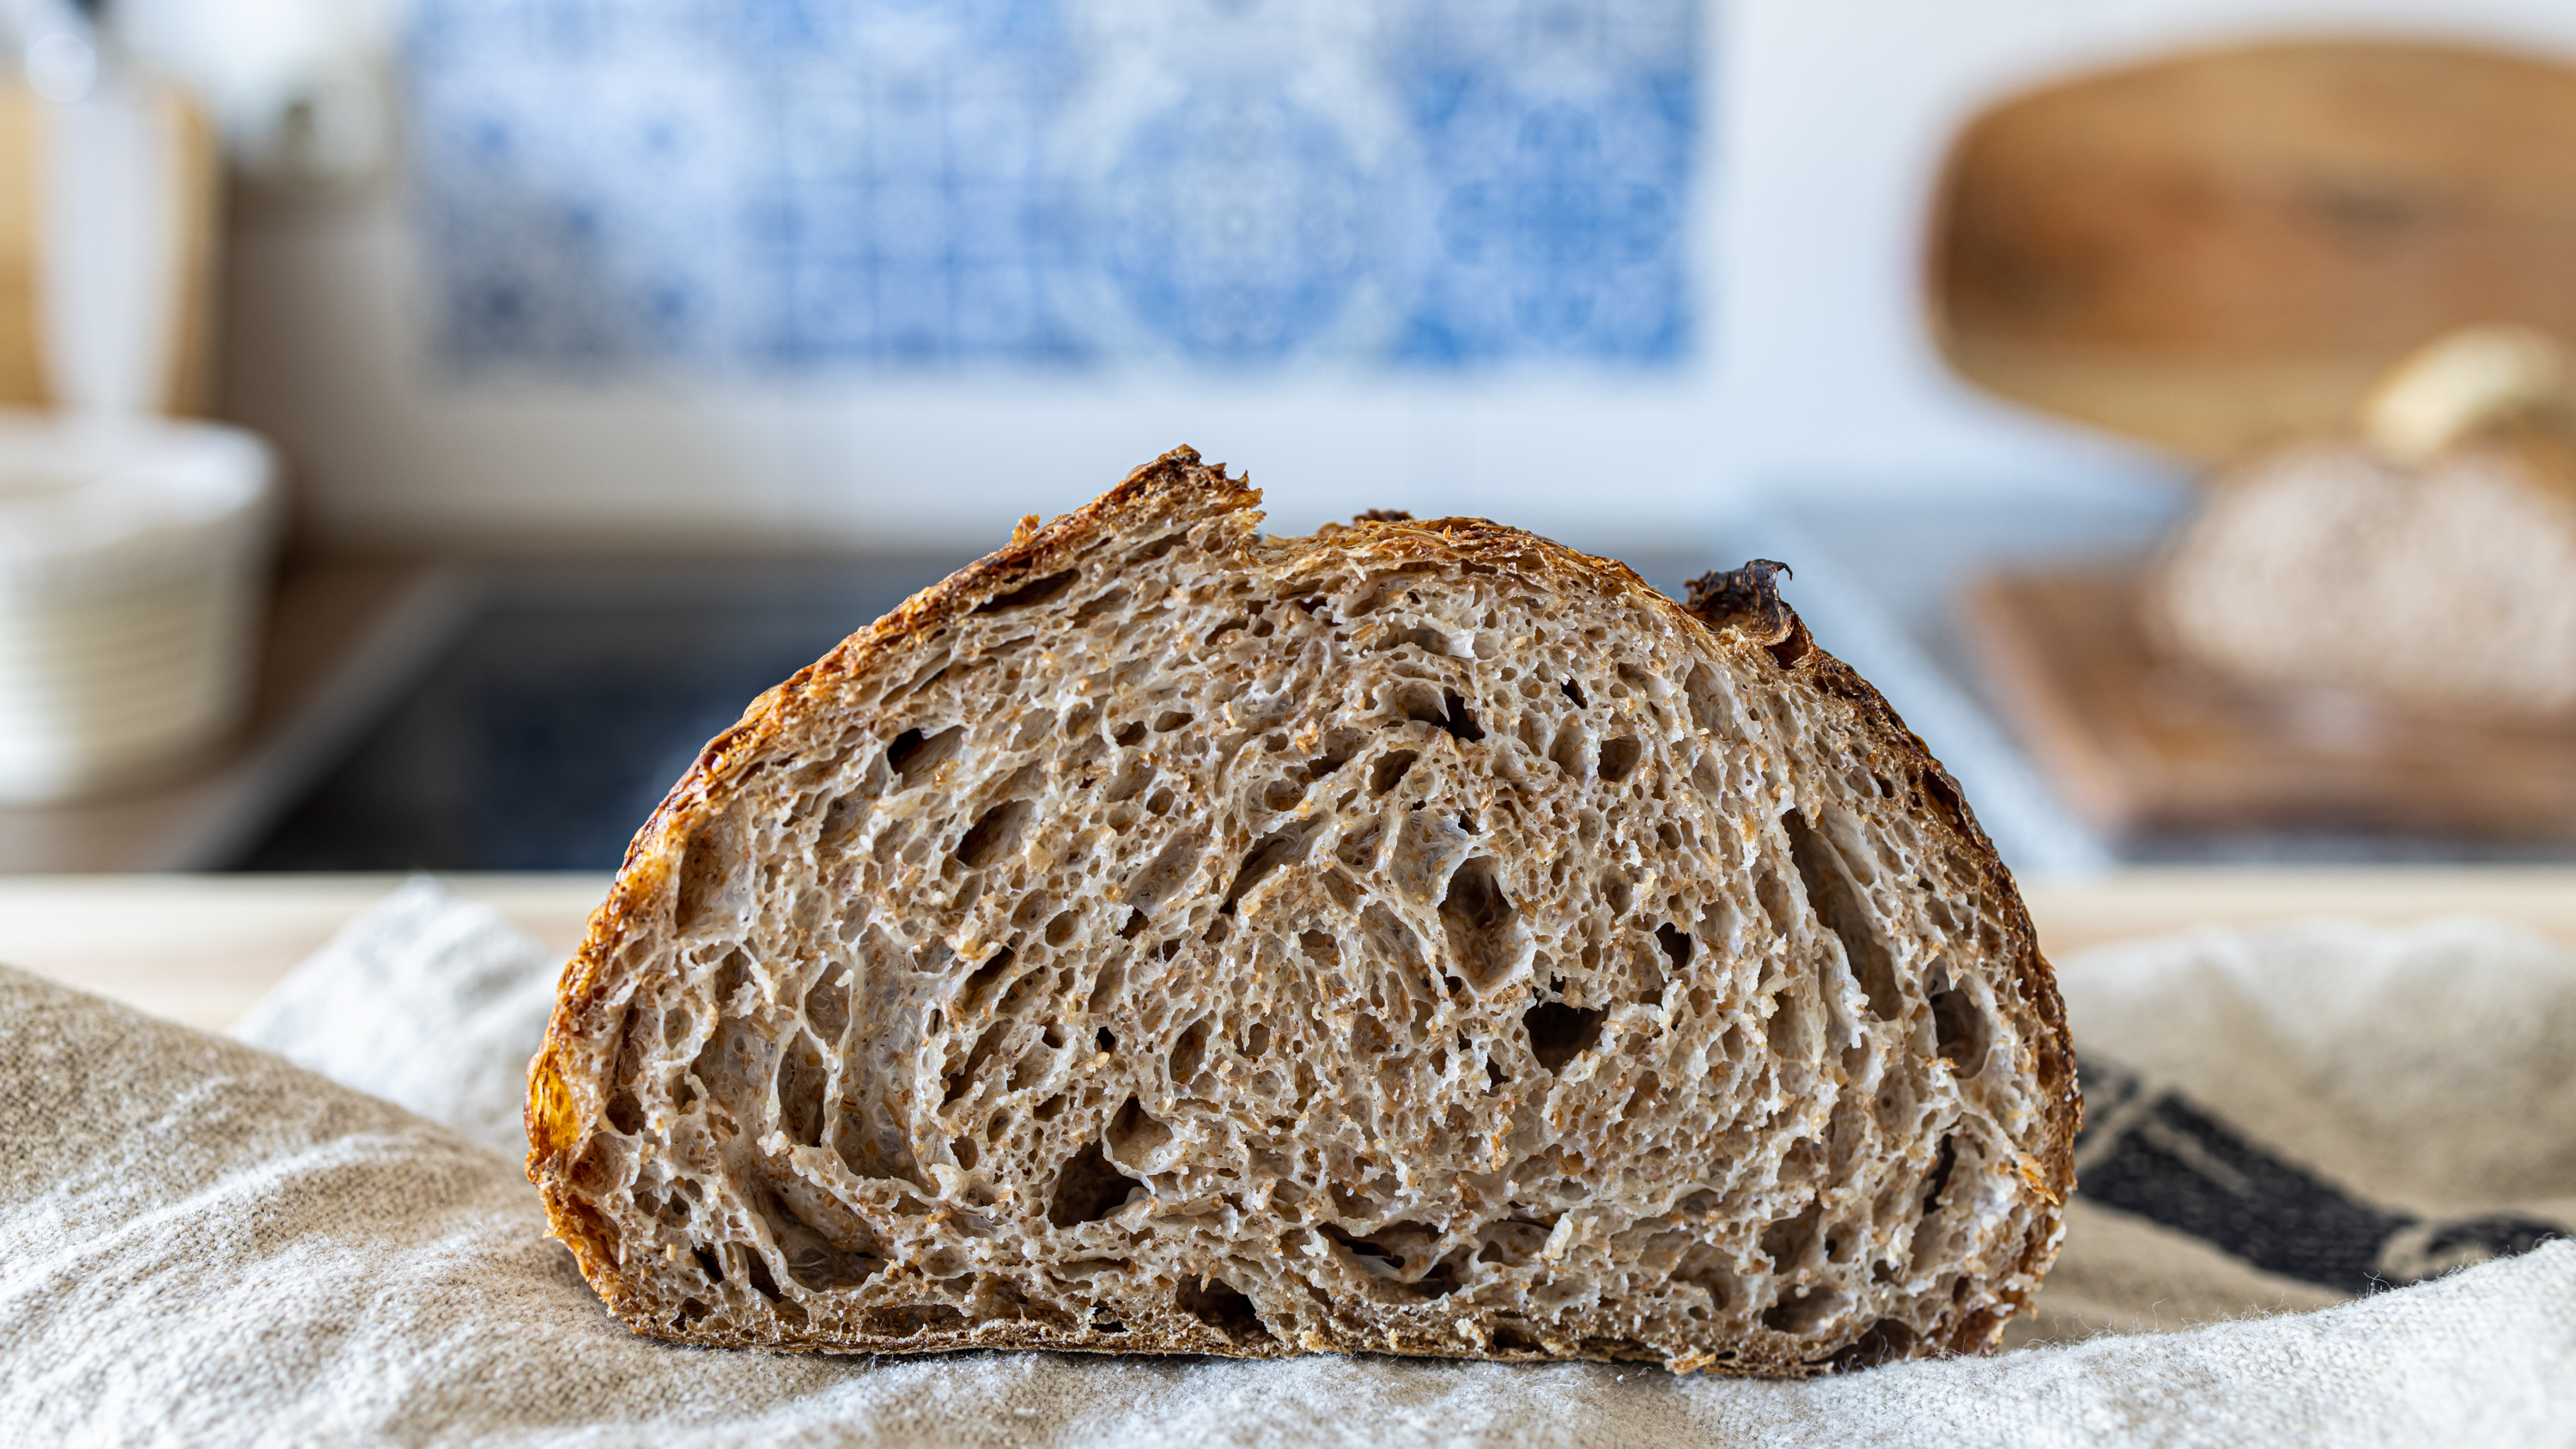
\includegraphics[width=\textwidth]{whole-wheat-crumb}
  \caption{A whole-wheat sourdough bread}
  \label{whole-wheat-crumb}
\end{figure}


By understanding the two key enzymes \textit{amylase} and \textit{protease}, you
will be better equipped to make bread to your liking. Do you prefer a softer
or stiffer crumb? Do you desire a lighter or darker crust? Do you wish to reduce
the amount of gluten in your final bread? These are all factors that you can
tweak just by adjusting the speed of your dough's fermentation.

\section{Yeast}

Yeasts are single-celled microorganisms belonging to the fungi kingdom, and
spores that are hundreds of millions of years old have been identified by
scientists. There are a wide variety of species--so far, about 1,500 have been
identified. Unlike other members of the fungi kingdom such as mold, yeasts do
not ordinarily create a mycelium network \cite{molecular+mechanisms+yeast}
\footnote{For one interesting exception, skip ahead to the end of this
section.}.

\begin{figure}[!htb]
  \centering
  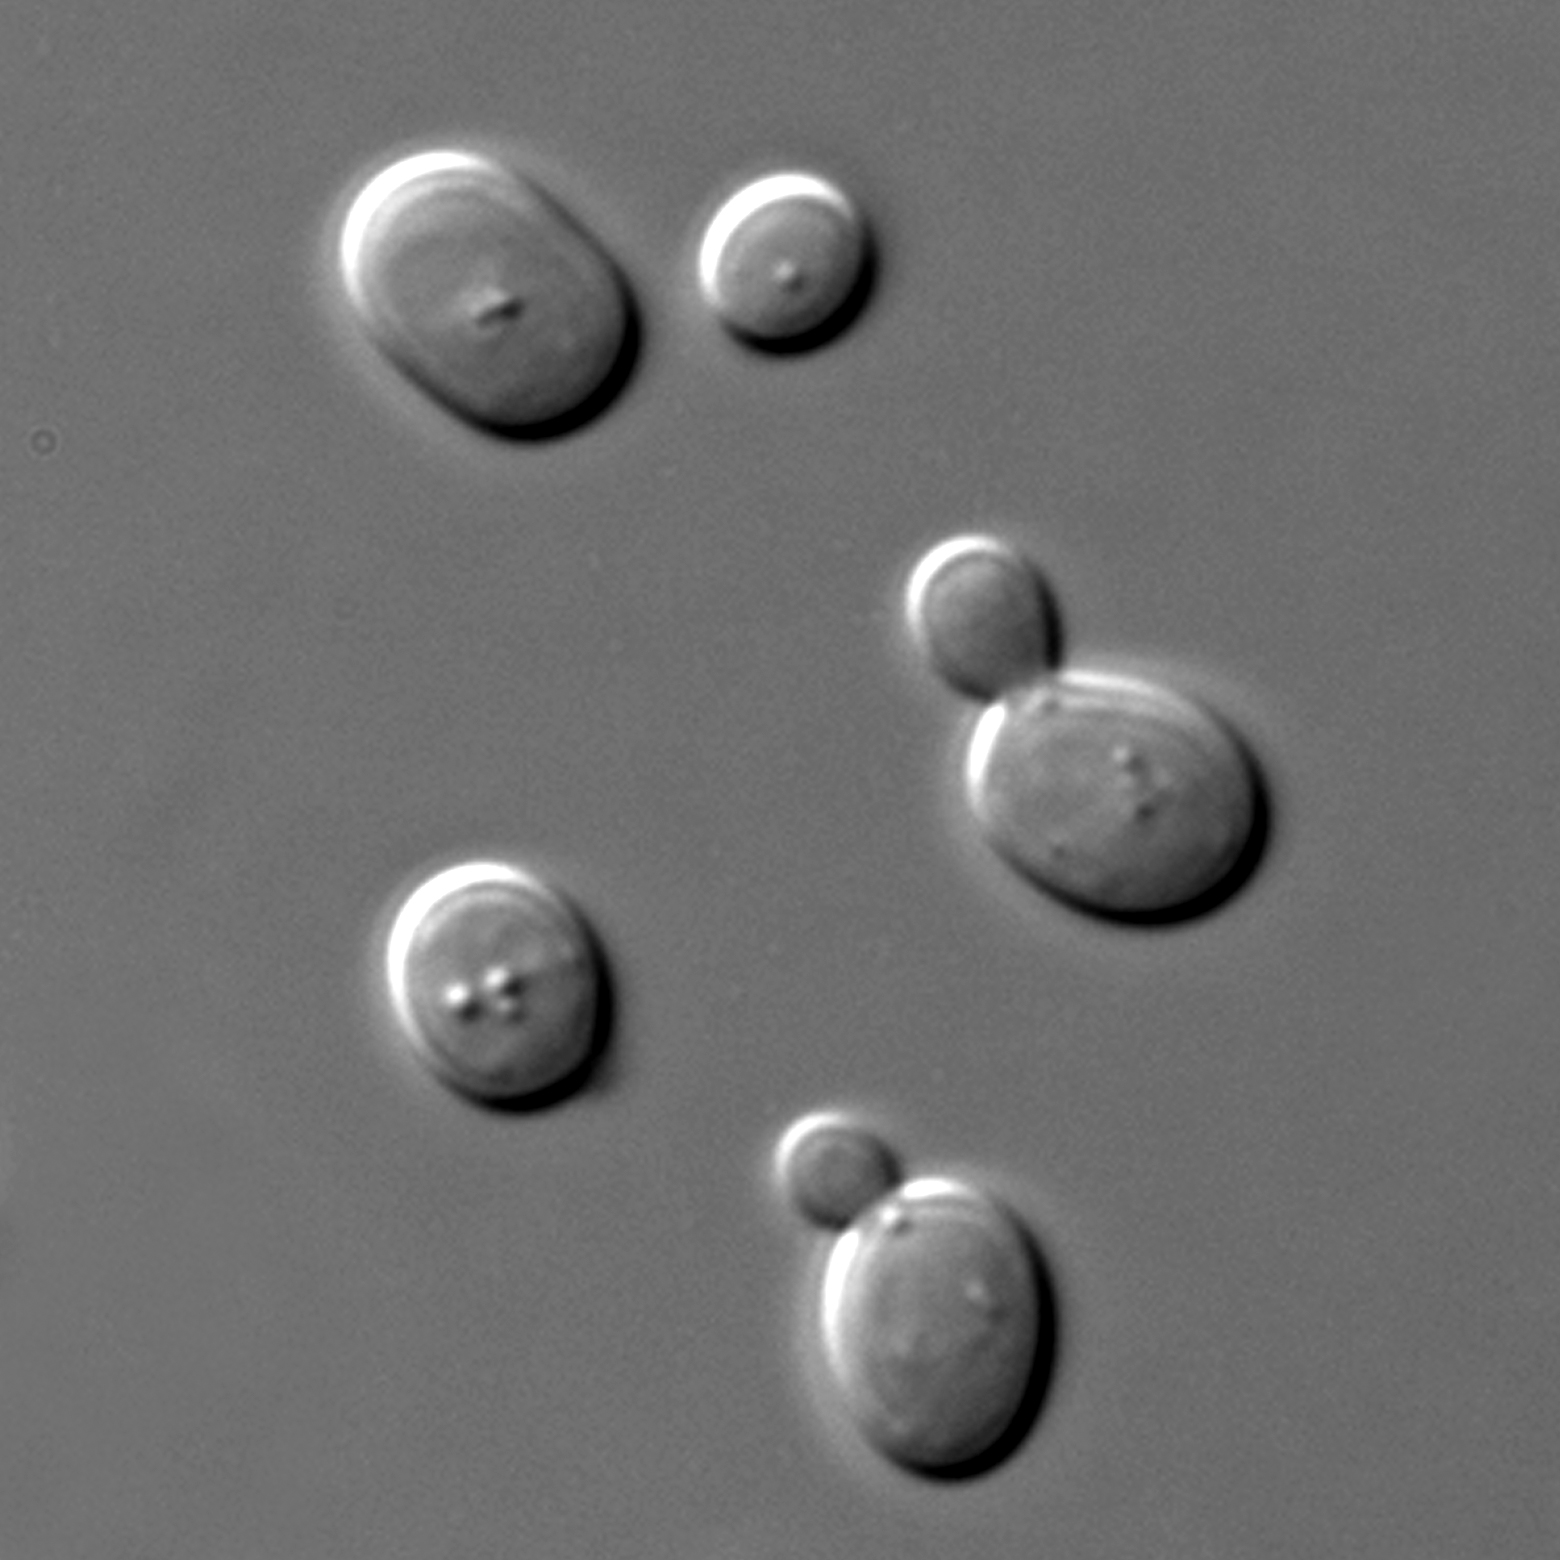
\includegraphics[width=1.0\textwidth]{saccharomyces-cerevisiae-microscope}
  \caption{Saccharomyces cerevisiae: Brewer's yeast under the microscope}
  \label{saccharomyces-cerevisiae-microscope}
\end{figure}

Yeasts are saprotrophic fungi. This means that they do not produce their own
food, but instead rely on external sources that they can decompose and break
down into compounds that are more easily metabolized.

Yeast breaks down carbohydrates into carbon dioxide and alcohol in what we today
refer to as the fermentation process. This process has been known for thousands
of years and has been used since ancient times for the making of bread as well
as alcoholic beverages.

Yeast can grow and multiply under both aerobic and anaerobic conditions. When
oxygen is present, they produce carbon dioxide and water almost exclusively.
When oxygen is not present, their metabolism changes to produce alcoholic
compounds \cite{effects+oxygen+yeast+growth}.

The temperatures at which yeast grows varies. Some yeasts, such as
{\it Leucosporidium frigidum}, do best at temperatures ranging from -2°C to
20°C, while others prefer higher temperatures. In general, the warmer the
environment, the faster the yeast's metabolism. The variety of yeast
that you cultivate in your sourdough starter should work best within the range
of temperatures where the grain was grown and harvested. So, if you are from a
cooler place and cultivate a sourdough starter from a nordic rye variety,
chances are your yeast will prefer a colder environment.

As an example, beer makers discovered a beneficial yeast living in the cold
caves around the city of Pilsen, Czech Republic. This yeast has since become
known for producing excellent beers at lower temperatures and varieties of
these strains are now used for brewing popular lagers.

Yeasts in general are very common organisms. They can be found on cereal
grains, fruits, and many other plants in the soil. They can even be found
inside your gut! As it happens, the types of yeast we use for baking are
cultivated on the leaves of plants, though very little is known about the
ecology involved.

Plants are protected by thick cell walls that few fungi or bacteria can
penetrate. However, there are some species that produce enzymes capable of
breaking down those cell walls so they can infect the plant.

Some fungi and bacteria live inside plants without causing them any distress.
These are known as {\it endophytes}. Not only do they \textit{not} damage their
host, they actually live in a symbiotic relationship, helping the plants in
which they dwell to protect themselves from other pathogens that might also
come to infect them through their leaves. In addition to this protection, they
also help with water and heat stress, as well as the availability of nutrients.
In exchange for their service to their host plants, these fungi and bacteria
receive carbon for energy.

However, the relationship between endophyte and plant is not always mutually
beneficial, and sometimes, under stress, they become invasive pathogens and
ultimately cause their host to decay \cite{endophytes+in+plants}.

There are other microorganisms that, unlike endophytes, do not penetrate cell
walls but instead live on the plant's surface and receive nutrients from rain
water, the air, or other animals. Some even feed on the honeydew produced by
aphids or the pollen that lands on the surface of the leaves. Such organisms
are called \textit{epiphytes}, and included among them are the types of yeast
we use for baking.

Interestingly, when you remove external food sources, a large number of
epiphytic fungi and bacteria can still be found on the plant's surface,
suggesting that they must somehow be feeding directly from the plant.
Indeed, there is some research indicating that some plants intentionally release
compounds such as sugars, organic and amino acids, methanol, and various
salts along the surface. These nutrients would then attract the epiphytes that
live on the plant's surface.

Epiphytes are advantageous to a plant's survival, as they are provided with
enhanced protection against mold and other pathogens. Indeed, it is in the
best interest of the epiphytes to keep their host plants alive for as long as
possible \cite{leaf+surface+sugars+epiphytes}.

More research is conducted every day into ways that yeasts can be used as
biocontrol agents to protect plants, the advantage being that these bio-agents
would be food-safe as the relevant strains of yeast are generally considered
harmless to humans. The yeasts would grow and multiply on the leaves,
essentially shielding them from other types of mold. This could be a potential
game changer for vineyards that suffer from mildew.

Such bio-agents could also be used to shield plants against the psychoactive
ergot fungus, which likes to grow in colder, more humid environments and
poses a significant problem for rye farmers.
Lawmakers have recently reduced the amount of allowed ergot contamination in
rye flour because it infects the grain and makes it unfit for consumption due
to its high toxicity to the liver. Yeasts could help to mitigate ergot contamination.

There is another interesting experiment performed by Italian scientists that
shows how crucial yeasts could be in protecting our crops. First, they made
tiny incisions into some of the grapes on a vine. Then, they infected the
wounds with mold. Some incisions were only infected with mold. Others were also
inoculated with some of the 150 different wild yeast strains isolated from the
leaves. They found that when the wound was inoculated with yeast, the grape
sustained no significant damage \cite{yeasts+biocontrol+agent}.

Intriguingly, there was also an experiment performed that showed how brewer's
yeast could function as an aggressive pathogen to grapevines. Initially, the
yeast lived in symbiosis with the plants, but after the vines sustained heavy
damage, the yeast became opportunistic and started to attack, even going so far
as to produce hyphae, the mycelium network normally associated with a fungus,
so that they could penetrate the tissue of the plants.

\section{Bacteria}

The other most dominant microbial antagonists in your sourdough are bacteria.
In fact, they are so dominant that they outnumber the yeast in your dough 100
to 1. Whereas yeast provides leavening power, bacteria create the distinct
flavours for which sourdough has been named. These are due to the acidic
byproducts that result from bacterial feeding. As a bonus, these acids
can significantly increase the shelf life of sourdough breads.
\cite{shelflife+acidity}

\begin{figure}
  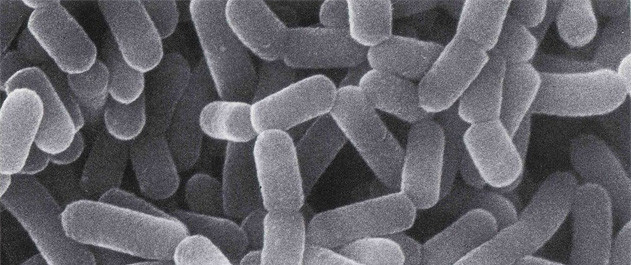
\includegraphics[width=1.0\textwidth]{bacteria-microscope}
  \caption{Fructilactobacillus Sanfranciscensis under the microscope}
  \label{lactobacillus-franciscensis-microscope}
\end{figure}

There are two predominant types of acid produced in sourdough bread: lactic and
acetic. In terms of flavor, lactic acid has clear dairy notes, while acetic
acid tastes of vinegar (of which it is, in fact, the primary ingredient!). These
acidic byproducts are produced by both \emph{homofermentative} and
\emph{heterofermentative} lactic acid bacteria.

\emph{Homofermentative} means that, during fermentation, the bacteria produce
a single compound: in this case, lactic acid. \emph{Heterofermentative}, on
the other hand, means that other compounds are also produced: in this case,
not only lactic acid, but also acetic acid, as well as ethanol and even some
carbon dioxide, two byproducts ordinarily associated with yeast. One quite
famous strain of lactic acid bacteria, \emph{Fructilactobacillus sanfranciscensis},
derives its name from the equally famous San Francisco style sourdough bread.
The first isolated culture came from a bakery in this city, hence the name.

Yeast and bacteria both compete for the same food source: sugar. Some scientists
have reported that bacteria consume mostly maltose, while yeast prefer glucose.
Others have reported that bacteria feed on the byproducts of yeast and vice
versa. This makes sense, as nature generally does a superb job of composting
and breaking down biological matter \cite{lactobacillus+sanfrancisco}.

I have yet to find a proper source that clearly describes the symbiosis between
yeast and bacteria, but my current understanding is that they both coexist and
sometimes benefit each other, but not always. Yeast, for example, tolerate the
acidic environment created by the surrounding bacteria and are thus protected
from other pathogens. Meanwhile, however, other research demonstrates that both
types of microorganisms produce compounds that prevent the other from
metabolizing food---an interesting observation, by the way, as it could help to
identify additional antibiotics or fungicides \cite{mold+lactic+acid+bacteria}.

In the past, I've tried cultivating mushrooms and observed the mycelium
attempting to defend itself against the surrounding bacteria; both types of
microorganisms actively produced compounds to combat each other. And yet,
after a while, the fight seemed to reach a standstill, as the mycelium had
fully grown around the bacterial patch, preventing it from spreading further.
I imagine a similar scenario could be playing out in our sourdough starters,
although, given that the sourdough environment tends to be more liquid, this
fight would have to take place everywhere in the dough and not just in an
isolated patch. More research on this topic is required to get a better understanding of
the details of the relationship between yeast and bacteria.


One other interesting trait of sourdough bacteria worth mentioning is their
ability to break down and consume the proteins in your dough. If you've baked
sourdough before, chances are you've experienced this firsthand. You'll recall
from the \emph{Enzymatic reactions} section that protease breaks down the
gluten network in your dough, resulting in a sticky mess if left unbaked for
too long. The bacteria, too, consume and break down the gluten in your
dough through a process called \emph{proteolysis}.

This, to me, was a great riddle when I first started working with sourdough.
On the one hand, it makes the dough stickier. On the other, it makes the dough
more extensible and easier to work with. As the gluten is reduced, the dough
becomes easier for the microorganisms to inflate, allowing it to rise. This
could be likened to the level of effort required to inflate a thick rubber tire
versus a thin and fragile balloon. The latter would be easy to blow up with
your mouth, while the former would not.

Unsurprisingly, proteolysis is further accelerated by the protease enzyme
previously discussed, which aids in the breakdown of gluten into smaller,
more easily metabolized amino acids.

This, to me, is the amazing process of fermentation. When you eat sourdough
bread, you are not merely consuming flour and water but the end result of
complex biological processes accomplished by the bacteria and yeast. Because
of the added bacterial component, sourdough bread typically contains less
gluten than a pure yeast-based dough \cite{proteolysis+sourdough+bacteria}.
Furthermore, the homofermentative bacteria metabolize the ethanol produced by
the yeast and other heterofermentative lactic acid bacteria. In both cases,
most of the resulting compounds are organic acids. Every natural resource in
your sourdough bread is recycled by the microorganisms inside, who are all
trying to eat whatever is available for as long as possible, and with each
feeding, they become more adept at utilizing these resources.

Depending on which flavour profile you prefer, you can select for one organic
acid or another. Acetic acid production requires oxygen, and by depriving
your sourdough starter of it, you can boost the population of homofermentative
lactic acid bacteria. Over time they will become dominant and outcompete the
acetic acid-producing bacteria \cite{acetic+acid+oxygen}.

The optimal fermentation temperature of your lactic acid bacteria depends on
the strains you've cultured in your starter. Generally, they work best at the
temperature used to create your starter because you've already selected for
bacteria that thrive under that condition.

In one noteworthy experiment, scientists examined the lactic acid bacteria
found on corn leaves. They lowered the ambient temperature from 20-25°C to around
5-10°C and afterward observed varieties of the bacteria that had never been
seen before \cite{temperature+bacteria+corn}, confirming that there is, in
fact, a large variety of bacterial strains living on the leaves of the plant.

Incidentally, you could perform a similar experiment by kicking off a sourdough
starter at a lower temperature. In theory, the microbiome should adapt, as the
microorganisms that thrive the most at lower temperatures will start to become
dominant. It would be interesting to see if this could actively influence the
taste of the resulting bread.

One last footnote worth mentioning: Some sources say that fermenting at a
lower temperature can increase acetic acid production, while fermenting at a
warmer temperature can boost lactic acid production. I could not verify this
in my own tests. More research is needed on the topic.

\chapter{Making a sourdough starter}
In this chapter you will learn how to make your
own sourdough starter. Before doing so you will
quickly learn about baker's math. Don't worry,
it's a very simple way how to write a recipe which
is cleaner and more scalable.  Once you get the hang
of it you will want to write every recipe this way.
You will learn to understand the signs to determine
your starter's readiness.  Furthermore you will
also learn how to prepare your starter for long-term storage.

\section{Baker's math}
\label{section:bakers-math}

In a large bakery, a determining factor is how
much flour you have at hand. Based on the amount
of flour you have, you can calculate how many
loaves or buns you can make. To make it easy
for bakers, the quantity of each ingredient
is calculated as a percentage based on how much flour you have.
Let me demonstrate this with a small example from
a pizzeria.  In the morning you check and you realize you
have around 1 kilogram of flour.
Your default recipe calls for around 600 grams of water.
That would be a typical pizza dough, not too dry but
also not too wet. Then you would be using around 20 grams
of salt and around 100 grams of sourdough starter.
\footnote{This is my go to pizza dough recipe. In Napoli
modern pizzerias would use fresh or dry yeast. However
traditionally pizza has always been made with sourdough.}
The next day you suddenly have 1.4 kilograms of flour
at hand and thus can make more pizza dough. What do you do?
Do you multiply all the ingredients by 1.4? Yes you could,
but there is an easier way. This is where baker's math
comes in handy. Let's look at the default recipe with baker's
math and then adjust it for the 1.4 kilogram flour quantity.

\begin{table}[H]
\centering
\resizebox{\textwidth}{!}{%
\begin{tabular}{|l|r|r|}
\hline
\textbf{Ingredient}    & \multicolumn{1}{l|}{\textbf{Percent}} & \multicolumn{1}{l|}{\textbf{Calculation}}  \\ \hline
1000g flour            & 100\%                                     & 1000g of 1000g = 100\%                     \\ \hline
600g water             & 60\%                                      & 600g of 1000g = 60\%                       \\ \hline
100g sourdough starter & 10\%                                      & 100g of 1000g = 10\%                       \\ \hline
20g salt               & 2\%                                       & 20g of 1000g = 2\%                         \\ \hline
\end{tabular}%
}
\end{table}

Note how each of the ingredients is calculated as a percentage
based on the flour. The 100 percent is the baseline as the absolute
amount of flour that you have at hand. In this case that's 1000 grams
(1 kilogram).

Now let's go back to our example and add just the flour, as we have
more flour available the next day. As mentioned the next day
we have 1.4 kilograms at hand (1400 grams).

\begin{table}[H]
\centering
\resizebox{\textwidth}{!}{%
\begin{tabular}{|l|r|r|}
\hline
\textbf{Ingredient} & \multicolumn{1}{l|}{\textbf{Baker's math}} & \multicolumn{1}{l|}{\textbf{Calculated value}} \\ \hline
Flour               & 100\%                                      & 1400*1 = 1400g                                 \\ \hline
Water               & 60\%                                       & 1400*0.6 = 840g                                \\ \hline
Sourdough starter   & 10\%                                       & 1400*0.1 = 140g                                \\ \hline
Salt                & 2\%                                        & 1400*0.02 = 28g                                \\ \hline
\end{tabular}%
}
\end{table}

For each ingredient we calculate the percentage
based on the flour available (1400 grams). So for the water
we calculate 60 percent based on 1400. Open up your
calculator and type in 1400 * 0.6 and you have
the absolute value in grams that you should be using.
For the second day, that is 840 grams. Proceed and do the same
thing for all the other ingredients and you know
your recipe.

Let's say you would want to use 50 kilograms of flour
the next day. What would you do? You would simply proceed
and calculate the percentages one more time. I like this
way of writing recipes a lot. Imagine you wanted to make
some pasta. You would like to know how much sauce you should
be making. Now rather than making a recipe just for you, a
hungry family arrives. You are tasked with making pasta
for 20 people. How would you calculate the amount of sauce
you need? You go to the internet and check a recipe and then
are completely lost when trying to scale it up.

\section{The process of making a starter}

\begin{figure}[!htb]
  \includegraphics[width=\textwidth]{sourdough-starter.jpg}
  \caption{A very active sourdough starter shown by the bubbles in the dough}
  \label{fig:sourdough-starter}
\end{figure}

Making a sourdough starter is very easy. All you need
is a little bit of patience. The flour you should
use to setup your starter is ideally a whole flour.
You could use whole wheat, whole rye, whole spelt or
any other flour you have. In fact gluten free flours such
as rice or corn would also work. Don't worry, you can
change the flour later. Use whatever whole flour you
already have at hand.

Your flour is contaminated with millions of microbes. As explained
before in the chapter about wild yeast and bacteria, these
microbes live on the surface of the plant. That's why
a whole flour works better because you have more natural
contamination of the microbes you are trying to cultivate
in your starter. More of them live on the hull compared to the
endophytes living in the grain.

Simply weigh around 50 grams of flour and add another 50
grams of water. It doesn't have to be exactly 50 grams of both
water or flour. You could also be using less and/or simply eyeball
it. The values are just shown as a reference. Don't use chlorinated
water to setup your starter. It should be bottled water ideally,
or here in Germany we can just use our tap water. The hydration
of your dough is 100 percent. This means you have equal parts
of flour and water. Stir everything together so that all the flour
is properly hydrated. By adding water many of your microbes'
spores become activated. They exit hibernation mode and
become alive again. Cover your mixture with a lid. I like to
use a glass and place another inverted one on top. The container shouldn't
be airtight. You still want some gas exchange to be possible.

\begin{figure}[!htb]
  \begin{tikzpicture}[node distance = 3cm, auto]
   	\node [block] (init) {\footnotesize Mix 50g flour + 50g water, stir}; 
	\node [block, right of=init, node distance=3cm] (wait1) {\footnotesize Wait 24 hours};
	\path [line] (init) -- (wait1);
	\node [block, right of=wait1, node distance=3cm] (feed) {\footnotesize 10g of previous day + 50g water + 50g flour, stir};
	\path [line] (wait1) -- (feed);
	\node [block, below of=feed] (discard) {\footnotesize Discard the rest};
	\path [line] (feed) -- (discard);
    \node [decision, right of=feed, node distance=3.5cm] (decide) {\footnotesize Is good?};
    \node [decision, above of=decide, node distance=3cm] (timeout) {\footnotesize Less than 10 feeds?};
	\node [block, above of=feed, node distance=3cm] (wait2) {\footnotesize Wait 24 hours};
    \node [block, right of=timeout, node distance=3cm] (discard2) {\footnotesize Batch failed};
	\path [line] (timeout) -- node{no} (discard2);
	\path [line] (timeout) -- node{yes} (wait2);
	\path [line] (feed) -- (decide);
    \node [block, right of=decide, node distance=3cm] (use) {\footnotesize Ready to use};
	\path [line] (decide) -- node{no} (timeout);
	\path [line] (wait2) -- (feed);
	\path [line] (decide) -- node{yes} (use);
  \end{tikzpicture}
  \caption{The process of making a sourdough starter from scratch}
  \label{fig:sourdough-starter-process}
\end{figure}

Now an epic battle begins. In one study scientists
have identified more than 150 different yeast species living
on a single leaf of a plant \cite{yeasts+biocontrol+agent}.
All of the different yeasts and bacteria are trying to get
the upper hand in this battle. Other pathogens such as mold
are also being activated as we added water. Only the strongest
most adaptable microorganisms will survive. By adding water to the
flour the starches start to degrade. The seedling tries to
sprout but it no longer can. Essential for this process is the
amylase enzyme. The compact starch is broken down to more
digestible sugars to fuel plant growth. Glucose is what the
plant needs in order to grow. The microorganisms that survive
this frenzy are adapted to consuming glucose. Luckily for us
bakers, the yeast and bacteria know very well how to metabolize
glucose. This is what they have been fed in the wild by the plants.
By forming patches on the leaf and protecting the plant from
pathogens they received glucose in return for their services.
Each of the microbes tries to defeat the other by consuming the
food fastest, producing agents to inhibit food uptake by others or by producing
bactericides and/or fungicides. This early stage of the starter
is very interesting as more research could possibly reveal
new fungicides or antibiotics. Depending on where your flour
is from, the starting microbes of your starter might be different
than the ones from another starter. Some people have also reported
how the microbes from your hand or air can influence your starter's
microorganisms. This makes sense to a certain extent. Your
hand's microbes might be good at fermenting your sweat, but
probably not so good and metabolizing glucose. The contamination
of your hands or air might play a minor role in the initial epic
battle. But only the fittest microbes fitting the sourdough's
niche are going to survive. This means the microorganisms that know
how to convert maltose or glucose will have the upper hand. Or the
microbes that ferment the waste of the other microbes. Ethanol created
by the yeast is metabolized by the bacteria in your sourdough. That's
why a sourdough has no alcohol. I can confirm the role of aerial
contamination to a certain extent. When setting up a new sourdough
starter the whole process is quite quick for me. After a few
days my new starter seems to be quite alive already. This might
be due to previous contamination of flour fermenting microbes in
my kitchen.

\begin{figure}[!htb]
  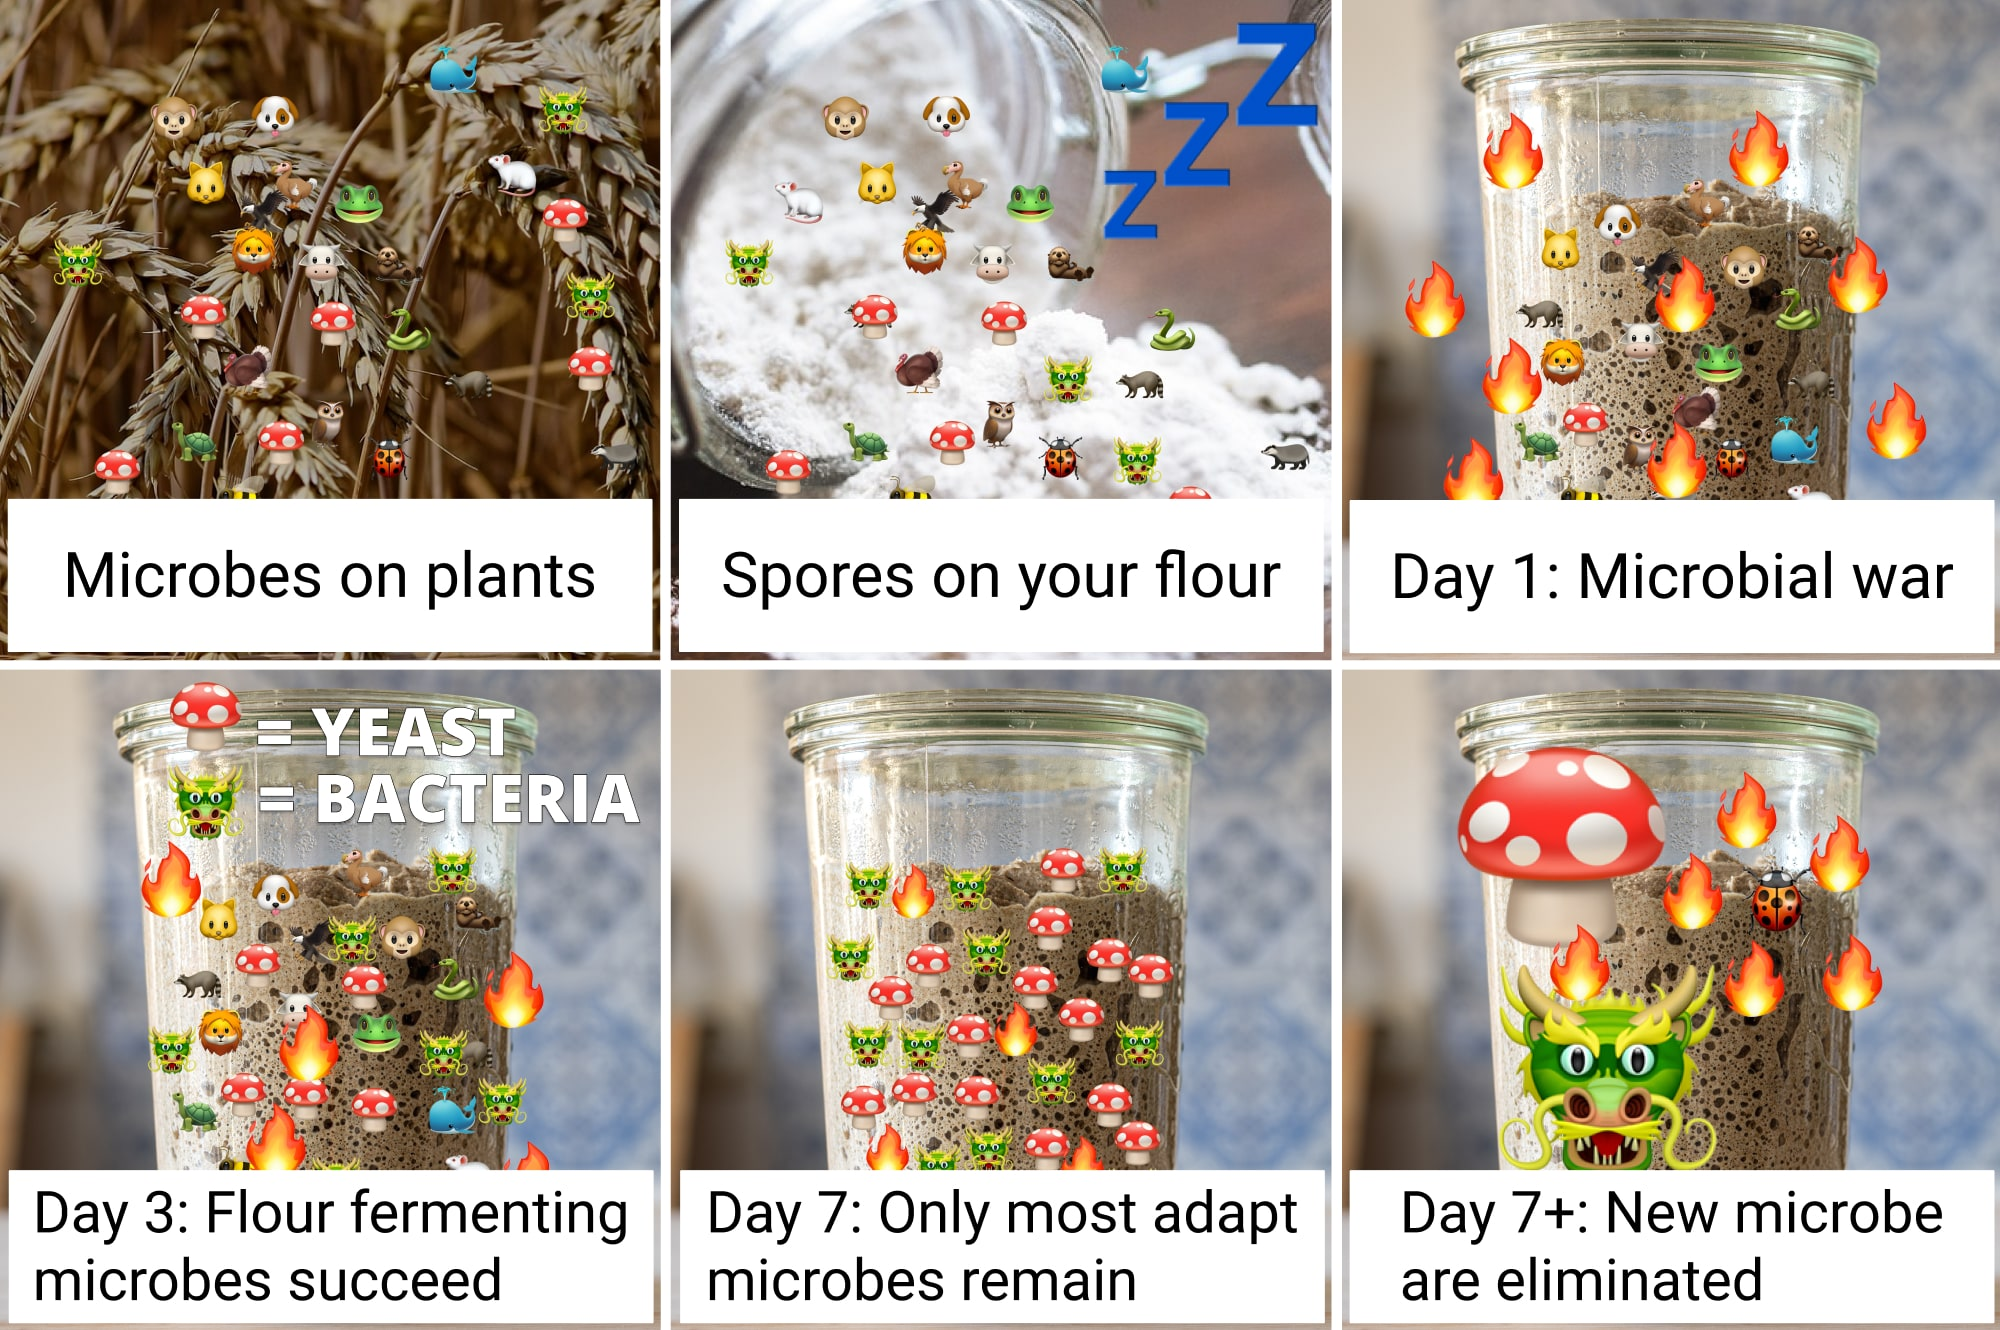
\includegraphics[width=\textwidth]{sourdough-starter-microbial-war}
  \caption{A simple visualization of the microbial warfare that happens during the making of a sourdough starter. The
  wild spores on the plant and flour become activated the moment flour and water is mixed.
  Only the most adapt flour fermenting microbes will survive. Because of unwanted microbial fermentation it is advised
  to discard the feeding-leftovers of the first days. The surviving yeast and bacteria continuously try to
  outcompete each other for resources. New microbes have a hard time entering the starter and are eliminated.
  }
  \label{fig:sourdough-starter-microbial-war}
\end{figure}

Wait for around 24 hours and observe what happens to your starter.
You might see some early signs of fermentation already. Use your nose
to smell the dough. Look for bubbles in the dough. Your dough
might already have increased in size a little bit. Whatever
you see and notice is a sign of the first battle. Some microbes
have already been outperformed. Others have won the first battle.
After around 24 hours most of the starch has been broken down
and your microbes are hungry for additional sugars. With a spoon
take around 10 grams from the previous day's mixture and place
it in a new container. Again - you could also simply eye ball
all the quantities. It does not matter that much. Mix the 10
grams from the previous day with another 50 grams of flour
and 50 grams of water. Note the ratio of 1:5. I very often use
1 part of old culture with 5 parts of flour and 5 parts of water.
This is also very often the same ratio I use when making a dough.
A dough is nothing else than a sourdough starter with slightly different
properties. I'd always be using around 100-200 grams of starter
for around 1000 grams of flour (baker's math: 10-20 percent).
Homogenize your new mixture again with a spoon. Then cover
the mix again with a glass or a lid. If you notice the top of
your mixture dries out a lot consider using another cover. The
dried out parts will be composted by more adapted microbes such as
mold. In many user reports I saw mold being able to damage
the starter when the starter itself dried out a lot. You will
still have some mixture left from your first day. As this contains
possibly dangerous pathogens that have been activated we will discard
this mixture. Once your sourdough starter is mature never
discard it. It's long fermented flour that is an excellent addon
used to make crackers, pancakes and or delicious hearty sandwich
breads. I also frequently dry it and use it as a rolling agent
for pizzas that I am making.

You should hopefully again see some bubbles, the starter increasing
in size and/or the starter changing its smell. Some people give
up after the second or third day. That is because the signs might no longer
be as dominant as they were on day one. The reason for this lies in only a few
select microbes starting to take over the whole sourdough starter. The most
adaptable ones are going to win. They are very small in quantity and will
grow in population with each subsequent feeding. Even if you see no signs
of activity directly, don't worry. There is activity in
your starter on a microscopic level.

24 hours later again we will repeat the same thing again until
we see that our sourdough starter is active. More on that in the
next section of this book.

\section{Determining starter readiness}

For some people the whole process of setting up a starter takes
only 4 days. For others it can take 7 days, for some even 20 days.
This depends on several factors including how good your wild microbes
are at fermenting flour. Generally speaking, with each feeding
your starter becomes more adapted to its environment. Your
starter will become better at fermenting flour. That's why
a very old and mature starter you receive from a friend might
be stronger than your own starter initially. Over time
your sourdough starter will catch up. Similarly, modern baking
yeast has been isolated like this from century old sourdough
starters.

\begin{figure}[!htb]
  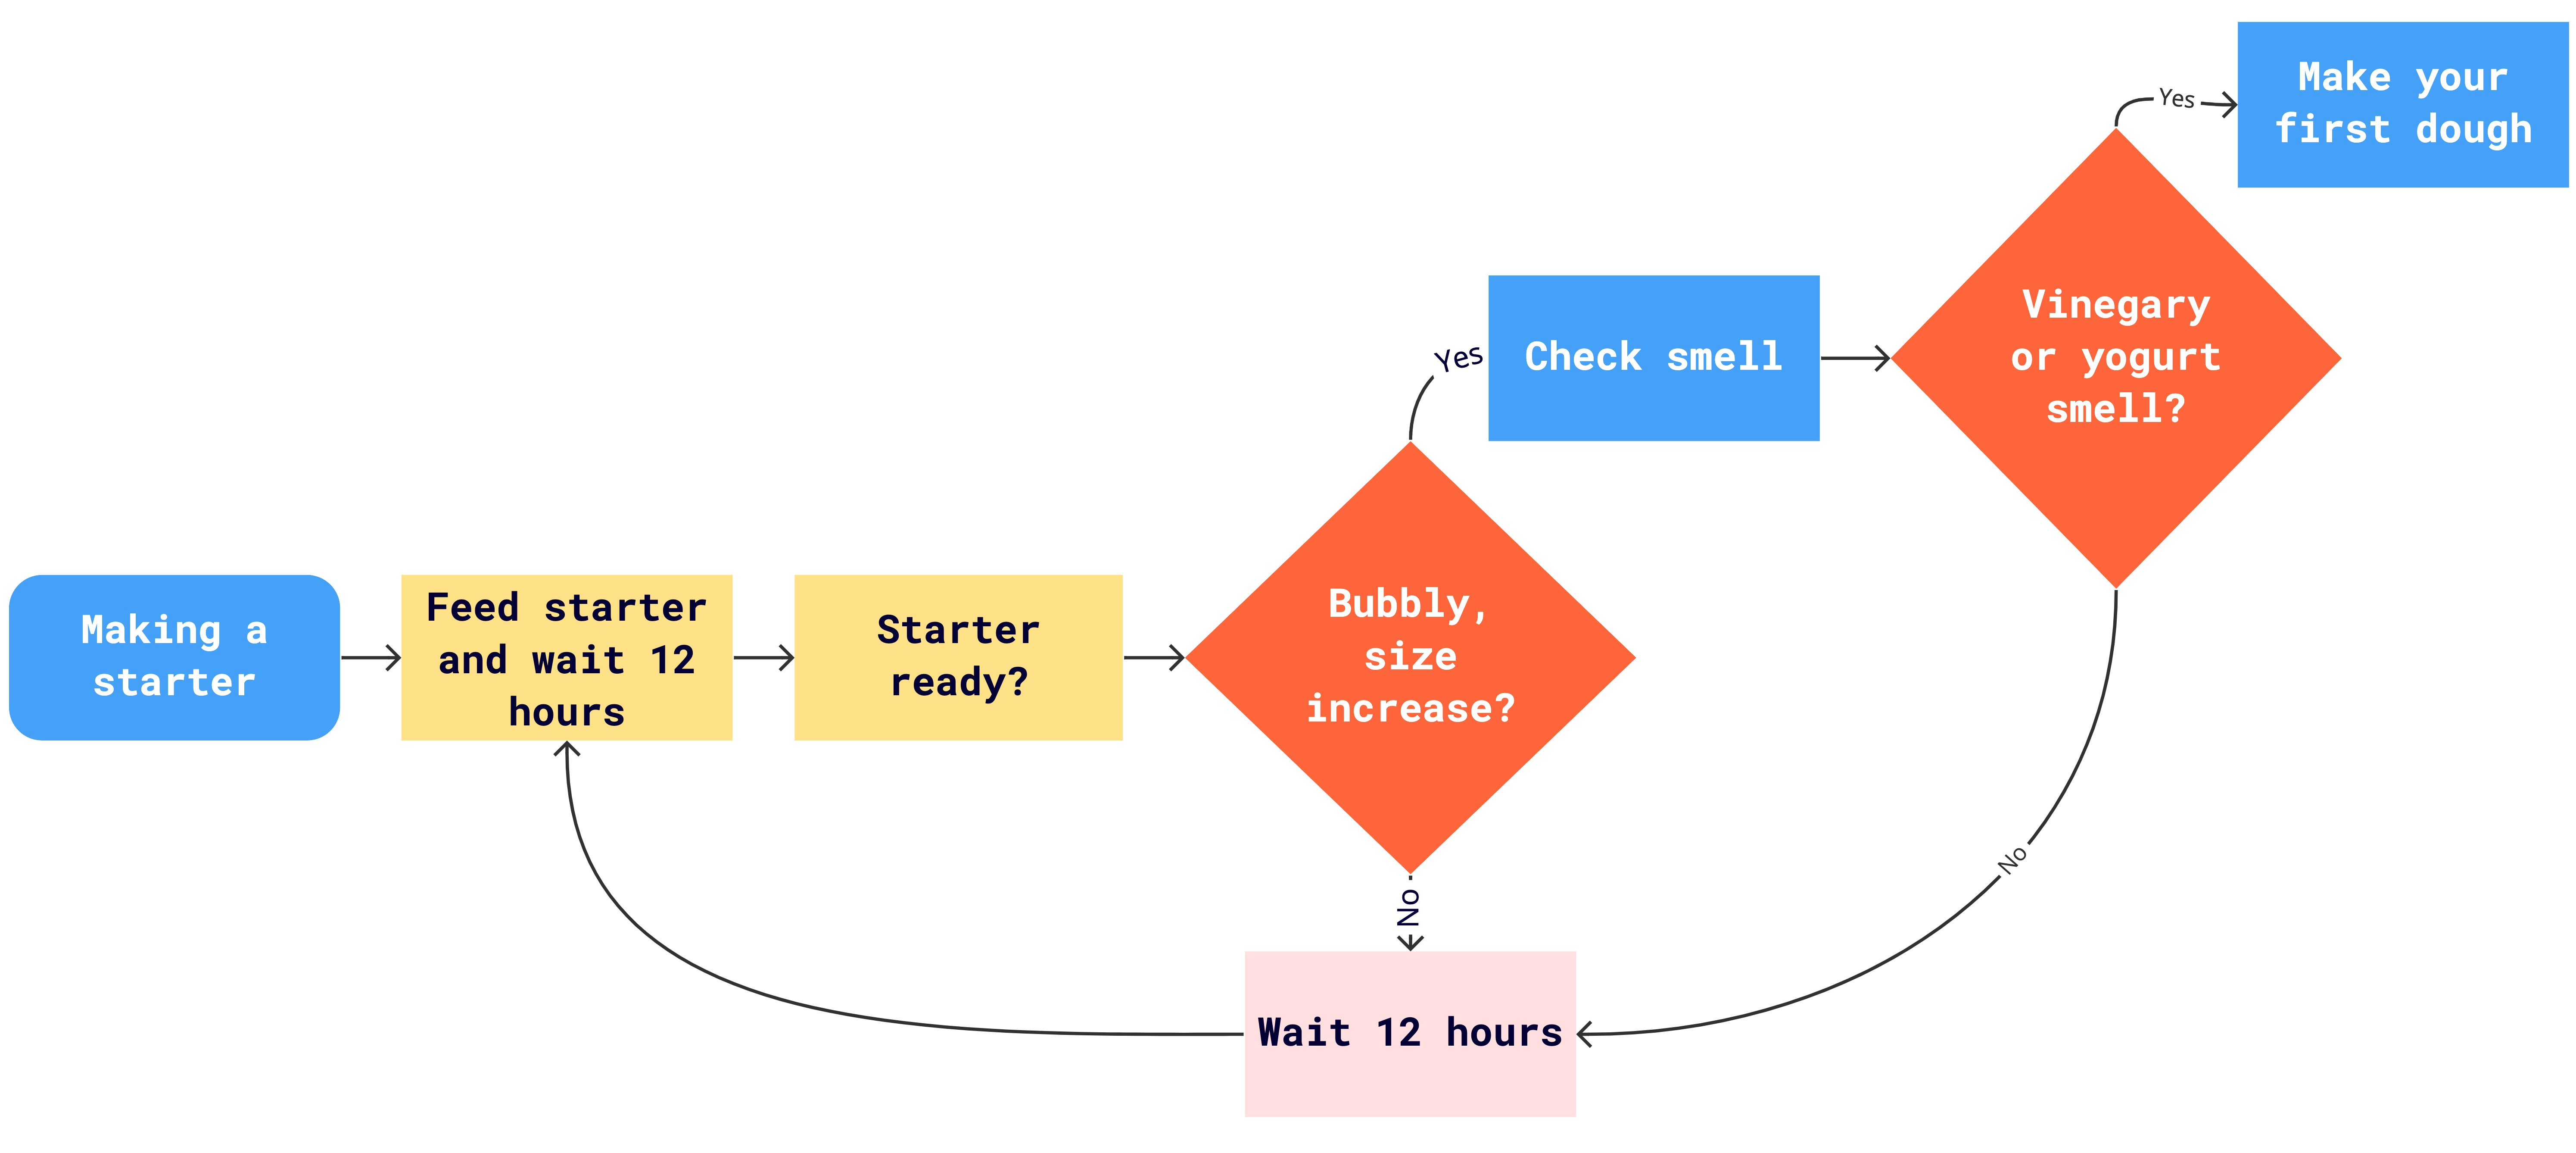
\includegraphics[width=\textwidth]{sourdough-starter-readiness.jpg}
  \caption{A flowchart showing how to check if your sourdough starter is ready
  to be used}
  \label{fig:sourdough-starter-readiness}
\end{figure}

The key signs to look at are bubbles that you see in your starter
jar. This is a sign that the yeast is metabolizing your
dough and creates CO2. The CO2 is trapped in your dough
matrix and then visualized on the edges of the container.
Also note the size increase of your dough. The amount of size
is irrelevant. Some bakers claim it doubles, triples or quadruples.
The amount of size increase depends on your microbes, but also on
the flour that you using to make the starter. A wheat flour contains
more gluten and will thus result in a higher size increase. At
the same time the microbes are probably not more active compared
to when living in a rye sourdough. You could only argue that
wheat microbes might be better at breaking down gluten compared
to rye microbes. That's one of the reasons why I decided to change
the flour of my sourdough starter quite often. I had hoped to create
an all-round starter that can ferment all sorts different flour.\footnote
{Whether this is actually working I can't scientifically say.
Typically the microbes that have once taken place are very strong
and won't allow other microbes to enter. My starter has initially
been made with rye flour. So chances are that the majority of
my microorganisms are from a rye source.} Your nose is also
a great tool to determine starter readiness. Depending on
your starter's microbiome you should notice either the smell
of lactic acid or acetic acid. Lactic acid has dairy yogurty notes.
The acetic acid has very strong pungent vinegary notes. Some
describe the smell as glue or acetone. Combining the visual clues
of size increase and pockets plus the smell is the best way
to determine starter readiness.

In rare events your flour might be treated and prevent microbe growth.
This can happen if the flour is not organic and a lot of biochemical
agents have been used by the farmer. In that case simply try again
with different flour. 7 days is a good period of time to wait before
trying again.

Another methodology used by some bakers is the so called \emph{float test}.
The idea is to take a piece of your sourdough starter and place it
on top of some water. If the dough is full with gas it will float
on top of the water. If it's not ready, it can't float and will
sink to the bottom. This test does not work with every flour.
Rye flour for instance can't retain the gas as well as wheat flour
and thus in some cases will not float. That's why I personally
don't use this test and can't recommend it.

Once you see your starter is ready I would recommend giving it
one last feeding and then you are ready to make your dough in the
evening or the next day. For the instructions to make your
first dough please refer to the next chapters in this book.

If your first bread failed, chances are your fermentation hasn't
worked as expected. In many cases the source is your sourdough starter. Maybe
the balance of bacteria and yeast isn't optimal yet. In that case a good
solution is to keep feeding your starter once per day. With each feeding your
starter becomes better at fermenting flour. The microbes will adapt more and
more to the environment. Please also consider reading the stiff sourdough starter
chapter in this book. The stiff sourdough starter helps to boost the
yeast part of your sourdough and balance the fermentation.

\section{Maintenance}

\begin{figure}[!htb]
  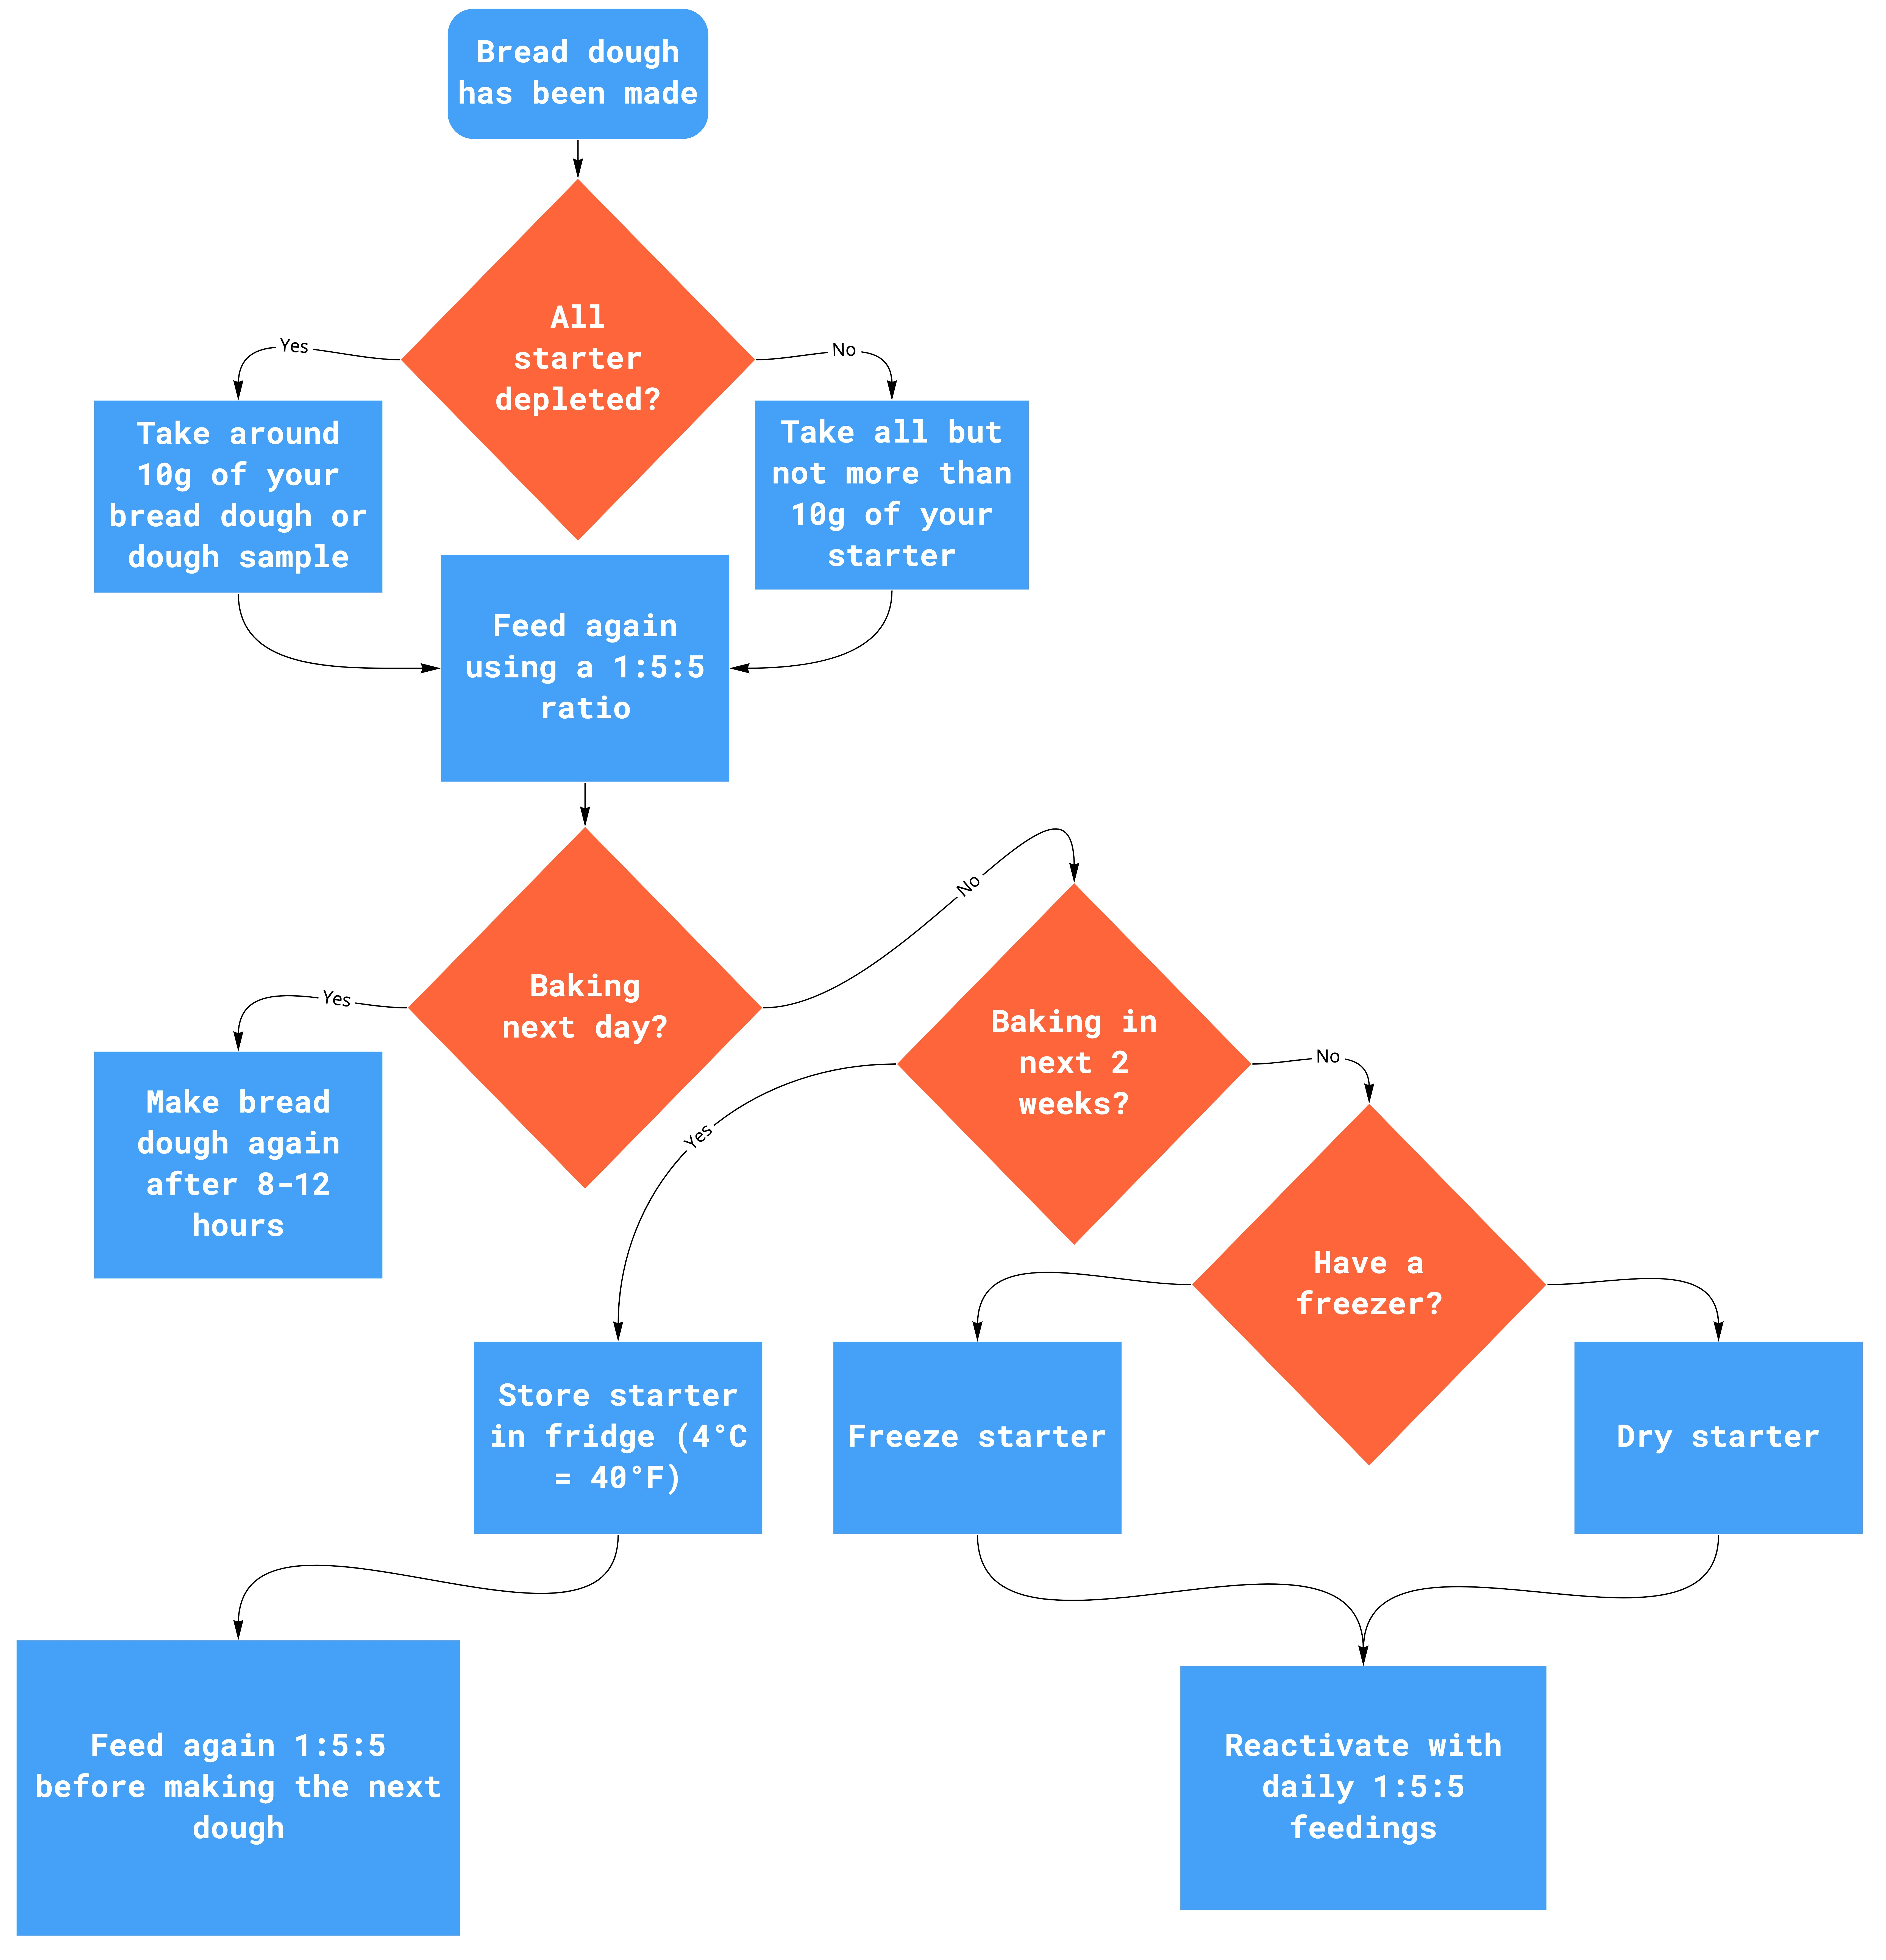
\includegraphics[width=\textwidth]{sourdough-starter-maintenance-process.jpg}
  \caption{A full flowchart showing how to conduct proper starter maintenance}
  \label{fig:sourdough-maintenance-process}
\end{figure}

You have made your sourdough starter and your first bread. How do you perform
maintenance for your starter? There are countless of different maintenance
methods out there. Some people go completely crazy about their starter and
perform daily feedings of the starter. The key to understanding how to properly
conduct maintenance is to understand what happens to your starter after you
used it to make a dough. Whatever starter you have left, or a tiny piece of
your bread dough can serve to make your next starter.\footnote{I very often use all my
starter to make a dough. So if the recipe calls for 50g of starter I make
exactly 50g starter in advance. This means I have no starter left. In that
case I would proceed to take tiny bit of the dough at the end of the
fermentation period. This piece I would use to regrow my starter again.}


As explained earlier your starter is adapted
to fermenting flour. The microbes in your starter are very resilient. They
block external pathogens and other microbes. That is the reason why, when
buying a sourdough starter, you will preserve the original microbes. They are
likely not going to change in your starter. They are outcompeting other
microbes when it comes to fermenting flour. Normally everything in nature
starts to decompose after a while. However the microbes of your starter have
very strong defense mechanisms. In the end your sourdough starter can be
compared to pickled food. Pickled food has been shown to stay good for a very
long period of time \cite{pickled+foods+expiration}. The acidity of your sourdough starter is quite
toxic to other microbes. The yeast and bacteria though have adapted to living
in the high acid environment. Compare this to your stomach, the acidity
neutralizes many possible pathogens. As long as your starter has sufficient
food available it will outcompete other microbes. When the starter runs out of
food the microbes will start to sporulate. They prepare for a period of no
food and will then reactivate the moment new food is present. The
spores are very resilient and can survive under extreme conditions.
Scientists have claimed they found 250 million year old spores that are still 
active \cite{old+spores}. While being spores
they are however more vulnerable to external pathogens such as mold.
Everything in nature is at some point decomposed and broken down by other
microorganisms. Under ideal conditions though the spores can survive for a
long time.

But as long as they stay in the environment of your starter they live
in a very protected protected environment. Other fungi and bacteria have a hard time decomposing your left over starter mass.
I have seen only very few cases where the starter actually died. It is almost impossible
to kill a starter.

What happens though is that the balance of yeast and
bacteria changes in your starter. The bacteria is more adapt to living
in the acidic environment. This is a problem when you make another dough.
You want to have the proper balance of fluffiness and sour notes.
When a starter has hibernated for a long period
of time, chances are that you do not have a desirable balance of microbes.
Furthermore depending on the time your starter hibernated you might only have
sporulated microbes left. So a couple of feedings will help to get your
sourdough starter into the right shape again.

The following are a couple of scenarios that will help you to conduct proper
starter maintenance, depending on when you want to bake the next time.

\textbf{I would like to bake again the next day:}

Simply take whatever starter you have left and feed it again. If you depleted
all your starter you can cut a piece of your dough. The dough itself is
nothing different than a gigantic starter. I recommend a 1:5:5 ratio like
mentioned before. So take 1 piece of starter, feed with 5 parts of flour and 5
parts of water. If it is very hot where you live, or if you want to make the
bread around 24 hours later after your last feeding, change the ratio. In that
case I would go for a 1:10:10 ratio. Sometimes I don't have enough starter.
Then I even use a ratio of 1:50:50 or 1:100:100. Depending on how much new
flour you feed it takes longer for your starter to be ready again.

\textbf{I would like to take a break and bake next week:}

Simply take your leftover starter and place it inside of your fridge. It will stay good
for a very long period of time. The only thing I see happening is the surface
drying out in the fridge. So I recommend to drown the starter in a little bit
of water. This extra layer of water provides a good protection from the top
part drying out. As mold is aerobic it can not grow efficiently grow under
water \cite{mold+anaerobic}. Before using the starter again simply either stir
the liquid into the dough or drain it. If you drain the liquid you can use it
to make a lacto fermented hot sauce for instance.

The colder it is the longer you preserve a good balance of yeast and
bacteria. Generally, the warmer it is the faster the fermentation process is, 
and the colder it is the slower the whole process becomes.
Below 4°C the starter fermentation almost completely stops. The
fermentation speed at low temperatures depends on the
strains of wild yeast and bacteria
that you have cultivated.

\textbf{I would like to take a several months break:}

Drying your starter might be the best option to preserve it in this case. As
you remove humidity and food your microbes will sporulate. As there is no
humidity the spores can resist other pathogens very well. A dried starter can
be good for years.

Simply take your starter and mix it with flour. Try to crumble the starter as
much as possible. Add more flour continuously until you notice that there is no
moisture left. Place the flour starter at a dry place in your house. Let it
dry even more. If you have a dehydrator you can use this to speed up the
process. Set it to around 30°C and dry the starter for 12-20 hours. The next
day return your starter. It is in a vulnerable state as there is still a bit
of humidity left. Add some more flour to speed up the drying process. Repeat
for another 2 days until you feel that there is no humidity left. This is
important or else it might start to mold. Once this is done simply store the
starter in an airtight container. Or you can proceed and freeze
the dried starter. Both options work perfectly fine. Your sporulated starter
is now waiting for your next feeding.

Initially it would take 3 days or so for my starter to become alive again
after drying and reactivating it. If I do the same thing now my starter is
sometimes ready after a single feeding. It seems that the microbes adapt. The ones
that survive this shock become dominant subsequently.

So in conclusion the maintenance mode you choose depends on when you want to bake next.
The goal of each new feeding is to make sure your starter
has a desired balance of yeast and bacteria when making a dough. There is no need to provide your
starter with daily feedings, unless it is not mature yet. In that case, each
subsequent feeding will help to to make your starter more adapt at fermenting
flour.


\chapter{Sourdough starter types}
In this chapter of the book we will have a closer look
at different sourdough starter types and their respective
traits.

\begin{table}[htp!]
  \includegraphics{tables/table-starter-types.pdf}
  \caption{A comparison of different sourdough starter types and their
  respective properties. The only difference is the level of water (hydration)
  that is used when feeding the starter.}
  \label{tab:starter-types-comparison}
\end{table}

Depending on the flour you have at hand, the type of starter changes. With more
bacterial activity you have more gluten consumption of your microbes. So if
you want to bake a free standing loaf, you need a flour with more gluten. The
more gluten you have, the more of it can be broken down whilst still maintaining
dough integrity. If you live in a country where the climate to grow wheat
isn't ideal and you only have weaker flours, then a stiff sourdough starter
could be advised. The stiff sourdough starter will improve yeast activity and
reduce bacterial activity. If you are a chaser of a very sour bread and have a
very strong wheat flour then you can try to play with a liquid sourdough
starter. The key difference between all of the starters is how much water
is used in the starter. The regular starter has a 1:1 relationship of flour
to water. The liquid starter has a 5:1 water-to-flour ratio, and the stiff
starter has half the flour as water.

\begin{figure}[!htb]
  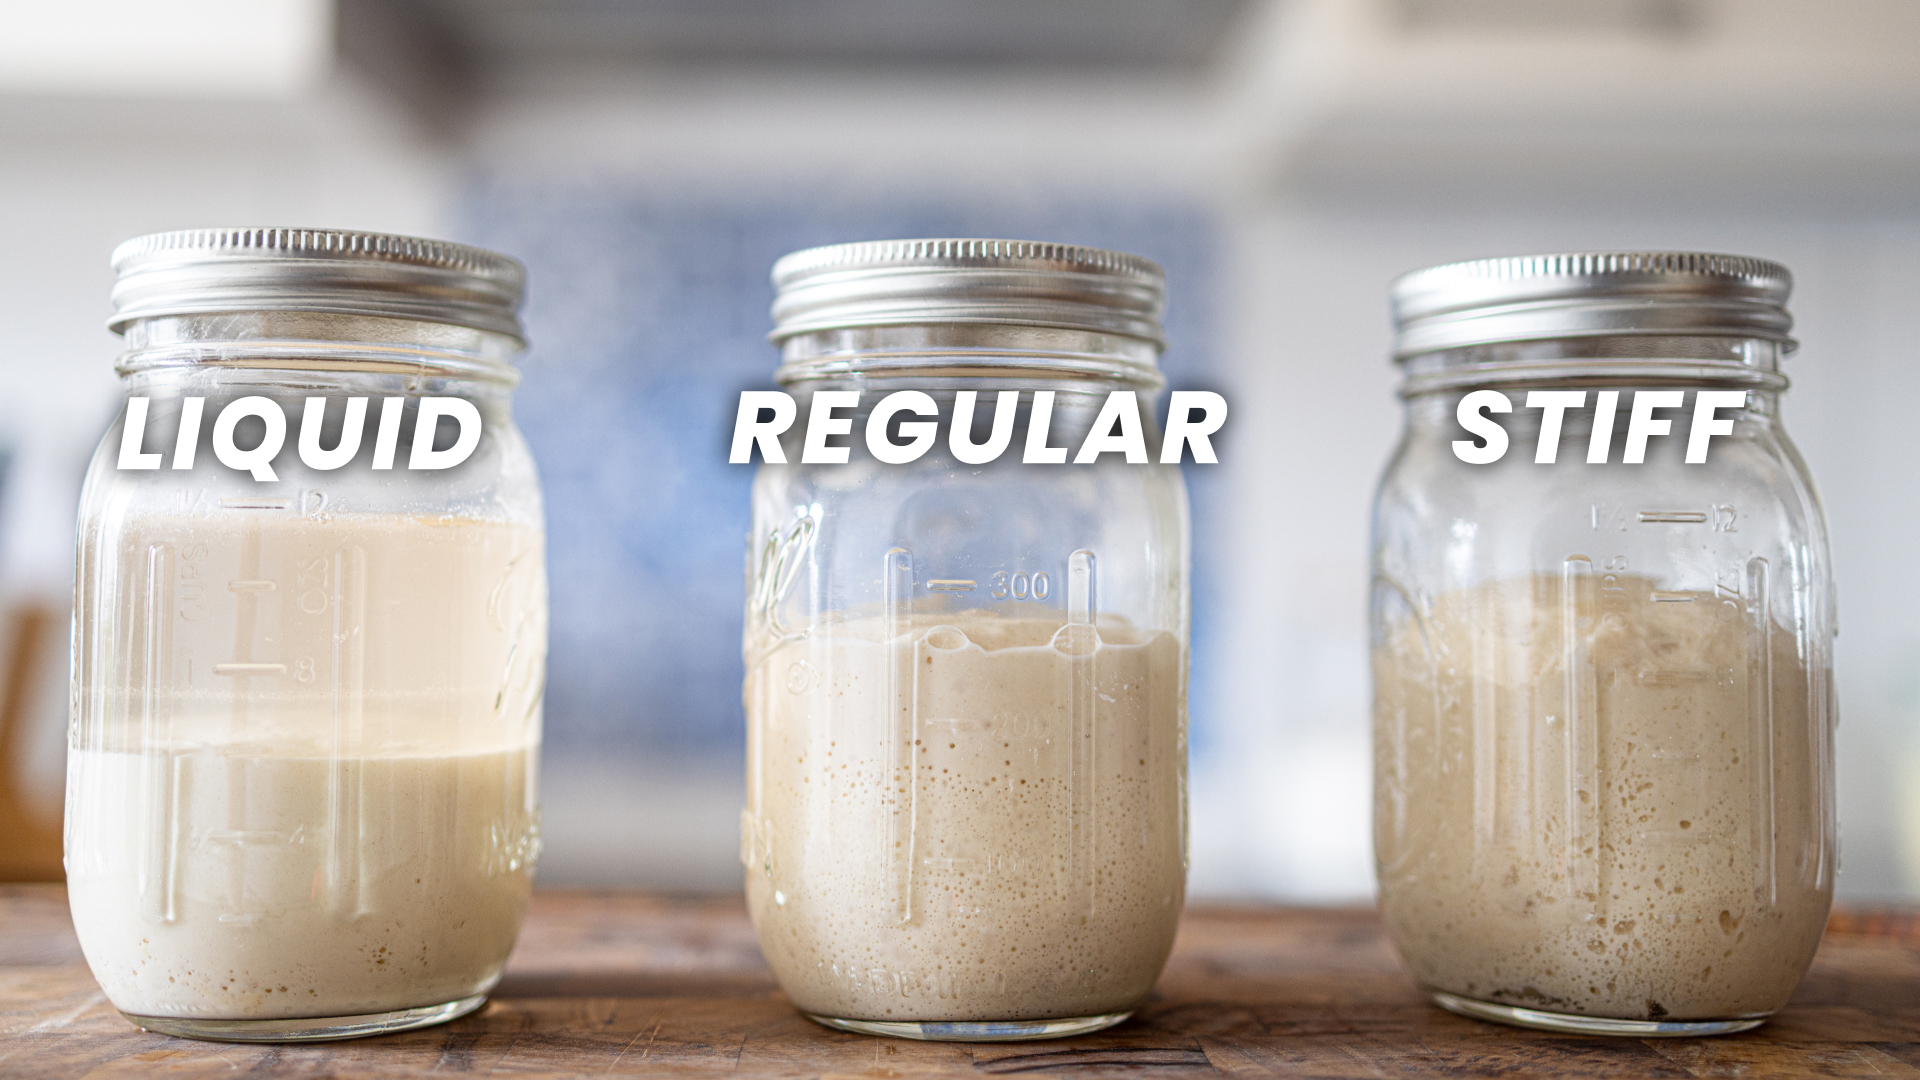
\includegraphics[width=\textwidth]{sourdough-starter-types}
  \caption{3 different starter types next to each other. Note how the liquid starter is submerged
  in water. It has a hydration of 500 percent or more.
  The regular starter has a hydration of around 100 percent, the stiff starter around 50 to 60 percent.}
  \label{fig:starter-types}
\end{figure}


You can change your starter type by just adjusting the feeding ratio of how
much flour and water you use. I frequently change my starter type from
regular to liquid and then back to a stiff starter. After changing the
environment of your microbes, apply feedings at the same ratio over a couple of
days so that they can adapt to the new environment. I typically see
changes after a single feeding, but I recommend 2 to 3 feedings, one feeding per
day, to see a stronger effect.

Your dough is generally just a big sourdough starter. So your starter is going
to adapt and regrow inside of your main dough. But you can influence the
properties that your starter carries over to your main dough. If you have more
bacterial fermentation, then your dough will also have slightly more bacterial
fermentation. If you have more yeast fermentation, then your main dough will
have slightly more yeast fermentation. This is important to know when you are
working with a more mature unfed starter. Let's say your starter had last been
fed 48 hours ago. Chances are that your bacteria is very active while the
yeast could be dormant. In such a case you can skip feeding your starter
before making another dough. Just use a very tiny amount of starter. For 1000 g
of flour I would take around 10 g of starter (1 percent in terms of baker's
math). If my starter is very young and had just been fed 6 to 8 hours ago I might
end up going up to 20 percent of starter. Remember that your dough is nothing
else other than a big starter. It will tremendously help you to figure out
your best next steps.

When using such a low inoculation rate (1 percent), you need to use stronger
flour when making wheat-based doughs. Your flour naturally breaks down due
to enzymatic activity. It might take 24 hours for the starter to re-grow
inside of your bread dough. At the same time, the enzymatic activity might
have caused your gluten to degrade significantly. While this is okay
when looking at your starter, your wheat-based dough will flatten
out during baking and no longer have the typical characteristics (fluffy crumb
structure). A stronger flour with more gluten is thus advised. It allows for
a longer fermentation before most gluten is broken down.

\section{Regular starter}

\begin{figure}[!htb]
  \includegraphics[width=\textwidth]{sourdough-starter.jpg}
  \caption{A regular sourdough starter at 100 percent hydration fed with rye flour}
  \label{fig:regular-sourdough-starter}
\end{figure}

The regular sourdough starter is made at a hydration of around 100 percent.
This means the starter has equal parts of flour and water. This is the most
common and must universal sourdough starter there is. The starter has a good
balance of yeast and bacteria. After a feeding, the volume increases and
increases. After it reaches a certain peak, it will start to collapse again.

The best way to judge whether the starter is ready is to look at signs such as
air pockets on the edges of your container. Also use the nose to evaluate the
smell of your starter. If you feel that the starter doesn't perform in a
desirable way, chances are that your yeast and bacteria ratios are off. In that
case frequent daily feedings using a 1:5:5 (starter:flour:water) ratio will
help.

A regular starter is a perfect choice to use when utilizing stronger wheat or spelt flours.
It also nicely works with rye, emmer or einkorn. If you only have a weak flour
at hand with less gluten, this starter might cause issues. As you tend to have
quite some bacterial activity, gluten is going to be broken down fast. When
using the starter, use around 1 to 20 percent starter based on the flour of your
dough.

Depending on the bacteria cultivated, a regular starter either has a lactic (dairy),
a vinegary (acetic) or mix of both flavor profiles. You can adjust your
starter's flavor by changing the type to a liquid starter.

\section{Liquid starter}
\label{section:liquid-starter}

\begin{figure}[!htb]
  \centering
  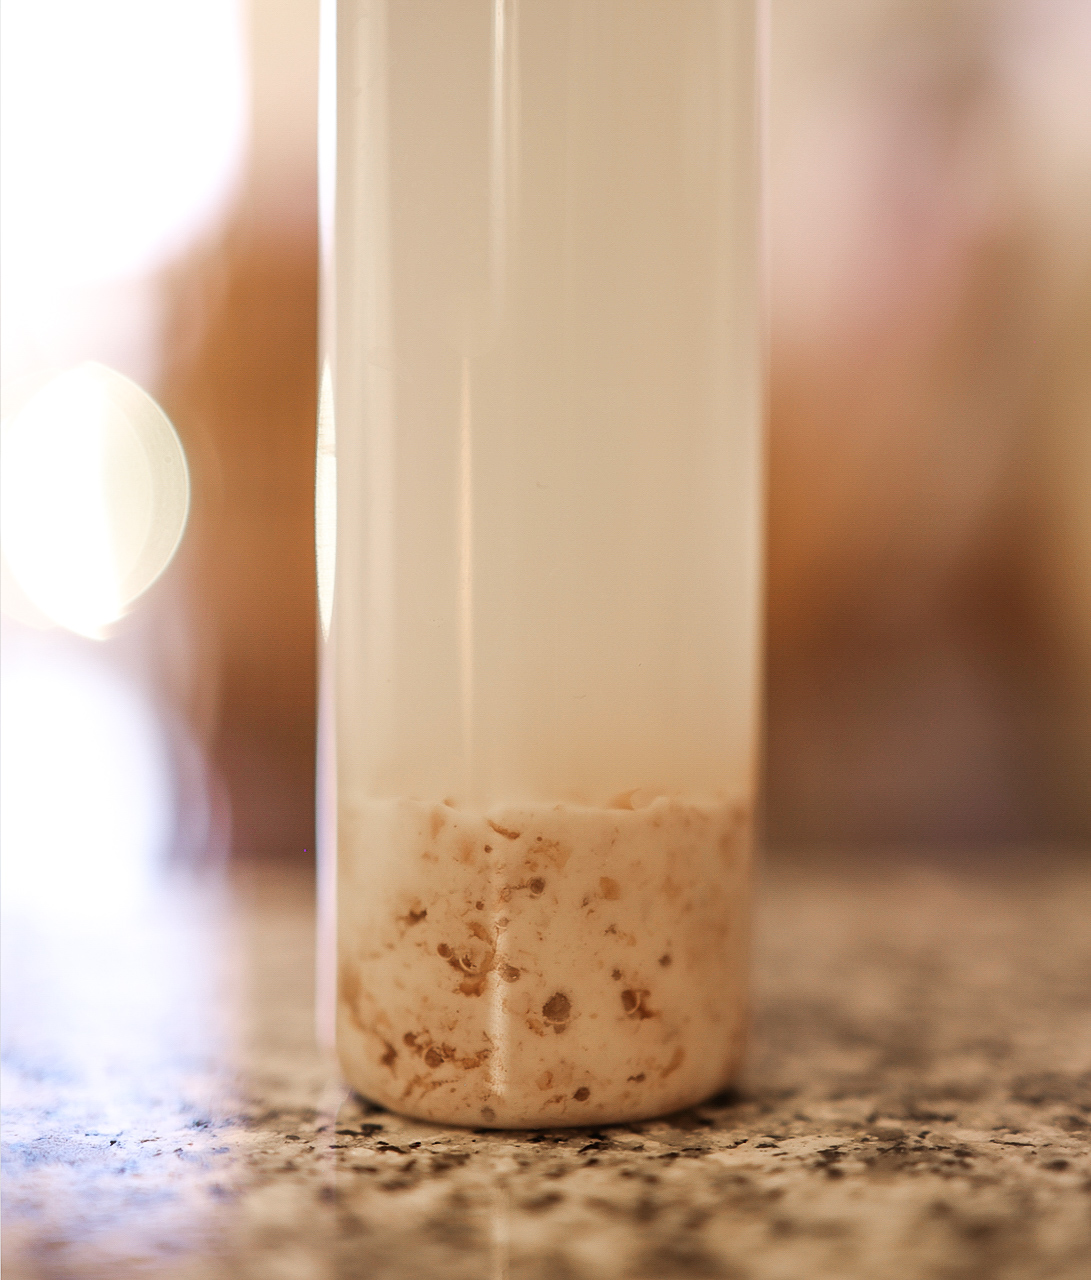
\includegraphics[width=0.5\textwidth]{sourdough-starter-liquid.jpg}
  \caption{A liquid sourdough starter features a high level of water. The high
  water amount boosts lactic acid producing bacteria. After a while the liquid
  and flour start to separate. Bubbles on the side of the flour
  indicate that the starter is ready to be used.}
  \label{fig:liquid-sourdough-starter}
\end{figure}


\begin{figure}[!htb]
  \includegraphics{figures/fig-liquid-starter-conversion.pdf}
  \caption{The process to convert your regular or stiff starter into a liquid starter. The whole
  process takes around 3 days. The longer you maintain your starter at the
  suggested hydration level, the more adapted your microorganisms become. It is recommended
  to keep a backup of your original starter as the liquid environment will select
  anaerobic microorganisms. This boosts bacteria that create lactic acid rather
  than acetic acid. The resulting acidity will be perceived as milder.}
  \label{fig:liquid-starter-conversion}
\end{figure}

The liquid starter is made at a hydration of around 500 percent. This means
the starter has much more water than flour. The additional layer of water on
top of the flour changes the microbiome of your starter.

By introducing this layer of water, less oxygen is available throughout the
course of fermentation. This means that your starter will no longer be
producing acetic acid. The heterofermentative lactic acid bacteria will thrive
in this environment. This is a neat little trick to change your starter's
flavor profile from vinegary to lactic. Your starter is going to develop
dairy creamy notes. Interestingly, when changing the hydration again, your starter
is going to maintain the liquid starter flavor profile, but then benefit again
from enhanced yeast activity. The liquid starter conversion is non reversible.
So ideally keep a backup of your stiff or regular starter.

To commence with the
conversion, simply take around 1 gram of your starter, mix with 5 g flour and
25 g water. Stir everything together properly. After a few minutes the flour is
going to start settling in at the bottom of your jar. Repeat this process over
a few days. Shake the starter gently to see if you can see tiny \ch{CO2} bubbles
moving in the liquid. This is a good sign that your starter is ready. Use your
nose to smell the starter. It should have a creamy dairy flavor note.

As you have more bacterial activity, this starter works best with a very strong
flour that can withstand a long fermentation period. Using this starter with a
weak wheat flour will not work. If you do not care about baking a freestanding loaf,
then you can easily use this starter together with a loaf pan.
This starter also works great when making a hearty pancake dough. To use it I
shake the starter container until I see all ingredients are homogenized. Then
I use around 5 percent of it in terms of baker's math. So for 1000 g of flour
that's around 50 grams of liquid starter. As it is very liquid you have to
include the 50 grams in your liquid calculation. I typically treat the starter
directly as liquid in the recipes. So if the recipe calls for 600 grams of water
and I use 50 grams of starter, then I would proceed and only use 550 grams of
water.

This type of starter is also an excellent mold combatant. As you are removing
oxygen from the equation, aerobic mold can not properly grow. If your starter
has a mold problem then the liquid conversion could be the remedy. Take a
piece of your starter where you suspect no mold growth. Apply the conversion
as mentioned before. The mold will likely sporulate as it runs out of food.
With each new feeding you are reducing the mold spores. The spores can no
longer reactivate as they can not do so in the anaerobic conditions.

The liquid on top of your starter is an excellent resource that you could use
to make sauces. If you feel you would like to add a little bit of acidity,
drain the liquid part on your starter and use it. I have used it numerous
times to make lacto-fermented hot sauces.

\section{Stiff starter}
\label{section:stiff-starter}

\begin{figure}[!htb]
  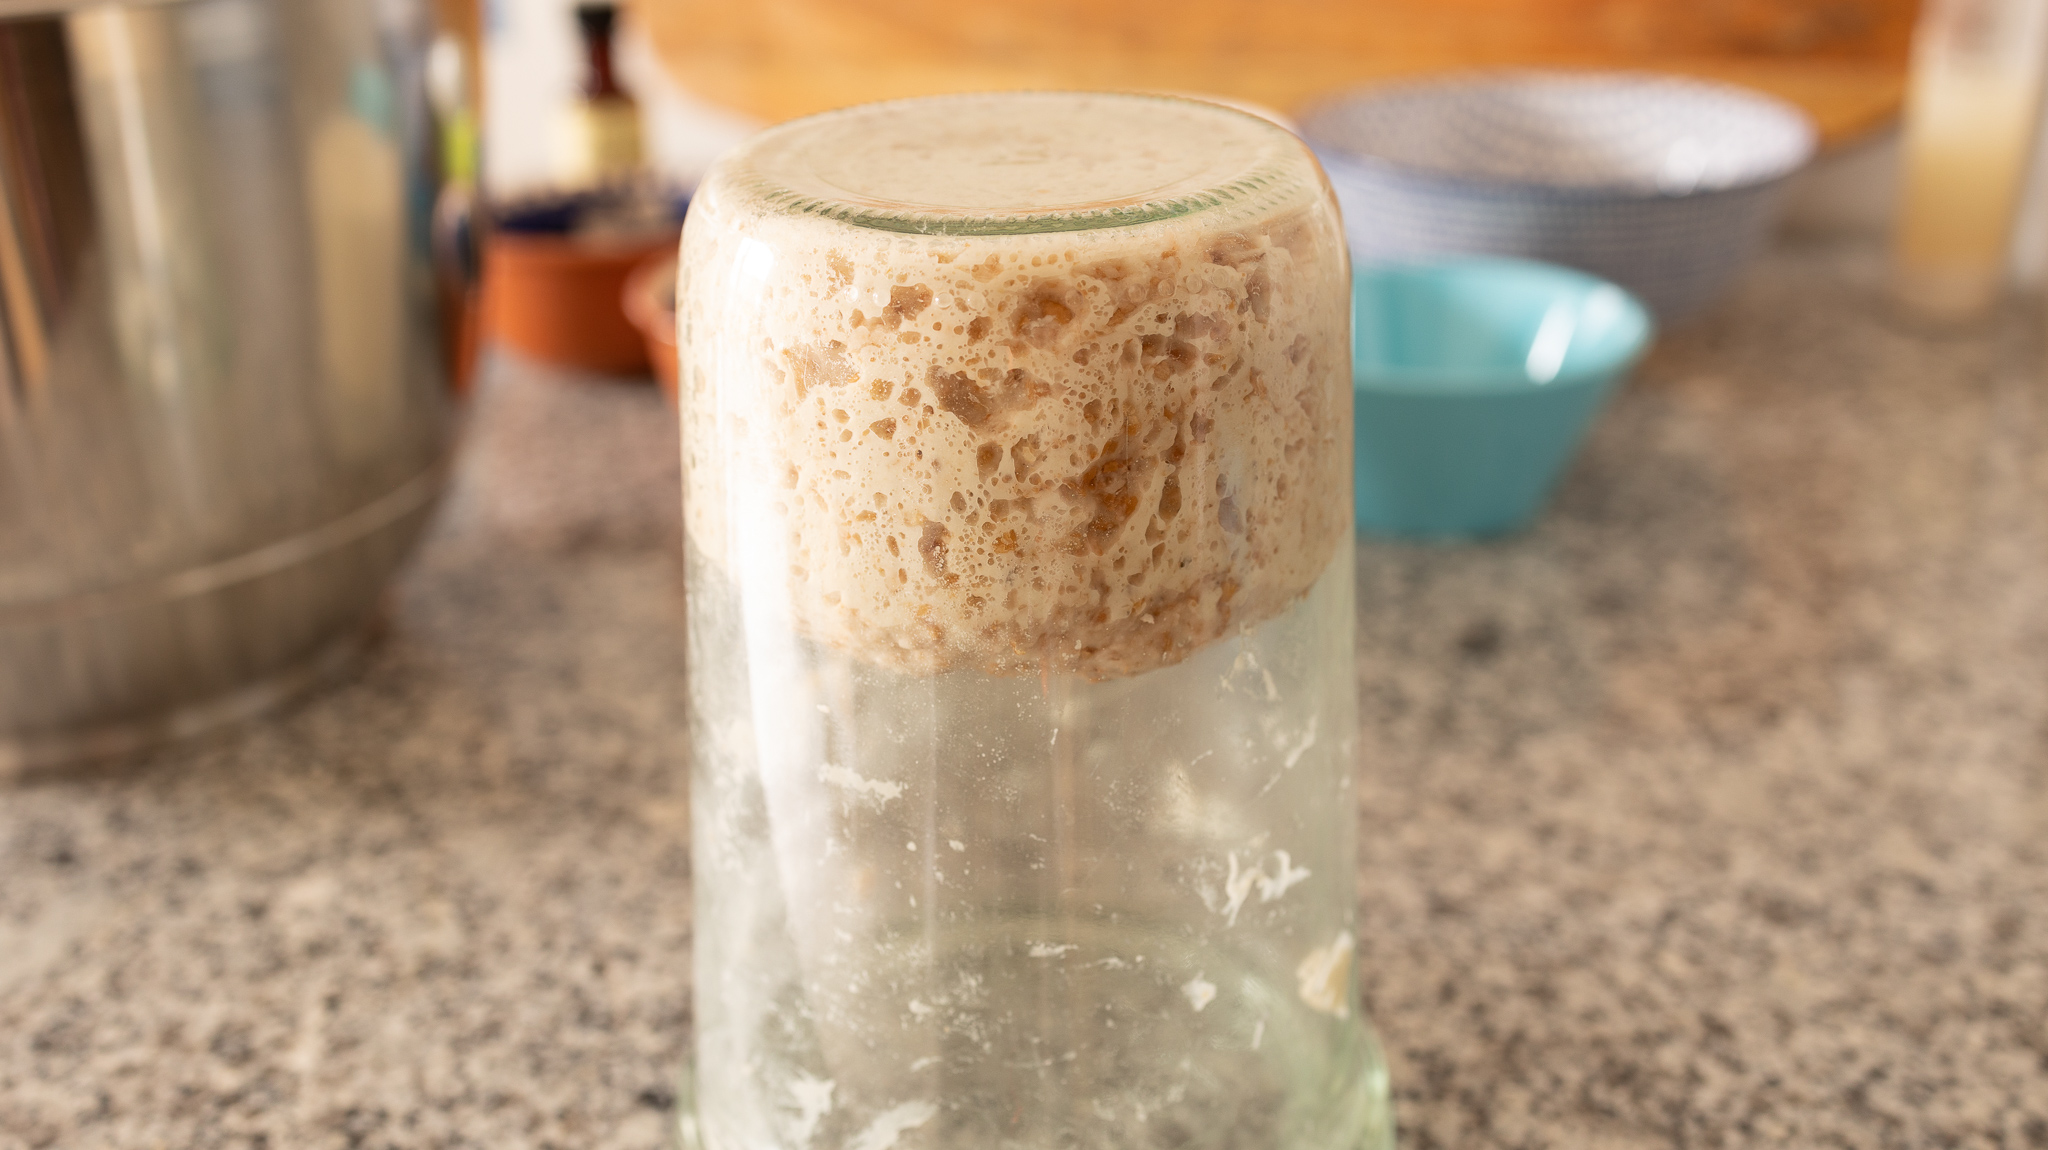
\includegraphics[width=\textwidth]{sourdough-starter-stiff.jpg}
  \caption{A stiff sourdough starter that I used to make a Stollen dough for Christmas. Note
  the bubbles on the edge of the container. The dough does not fall out of the jar.}
  \label{fig:stiff-sourdough-starter}
\end{figure}

The stiff starter is the driest of all the starters. It has a hydration of
around 50 to 60 percent. So for 100 grams of flour you are using around 50 to
60 grams of water. If you can't mix flour and water because the
mixture is too try you need to increase the water quantity. This is often
the case when using whole wheat flour to make your starter. The stiff
starter should have the consistency of pasta or pizza dough.

\begin{figure}[!htb]
  \includegraphics{figures/fig-stiff-starter-conversion.pdf}
  \caption{The process to convert your regular starter into a stiff starter. The whole
  process takes around 3 days. The longer you maintain your starter at the
  suggested hydration level, the more adapted your microorganisms become. The
  stiff starter boosts the yeast activity of your sourdough starter.
  The guide uses a 50 percent hydration level for the starter. If the dough is too stiff
  consider increasing this to 60 percent.}
  \label{fig:stiff-starter-conversion}
\end{figure}

In the stiffer environment the yeast thrives more. This means you will have
more \ch{CO2} production and less acid production. In my tests this is a game
changer especially if you are using weaker gluten flours. The wheat flours in
my home country of Germany tend to be lower in gluten. For wheat to build gluten, warm conditions
are preferred \cite{gluten+development+temperatures}. When following recipes from other bakers, I
could never achieve similar results. When following timings my doughs would
simply collapse and become super sticky. Only when I started to buy more
expensive wheat flour did my results start to change. As not everyone can afford
these special baking flours and due to their limited availability, I stumbled upon the
stiff sourdough starter. I made several tests where I used the same amount of
starter and flour. I only changed the hydration between all the starters. I
would then proceed and place a balloon on top of each of the jars. The stiff
starter jar was clearly inflated the most. The regular starter
followed in second place. The liquid starter finished in third place with far less \ch{CO2}
production.

\begin{figure}[!htb]
  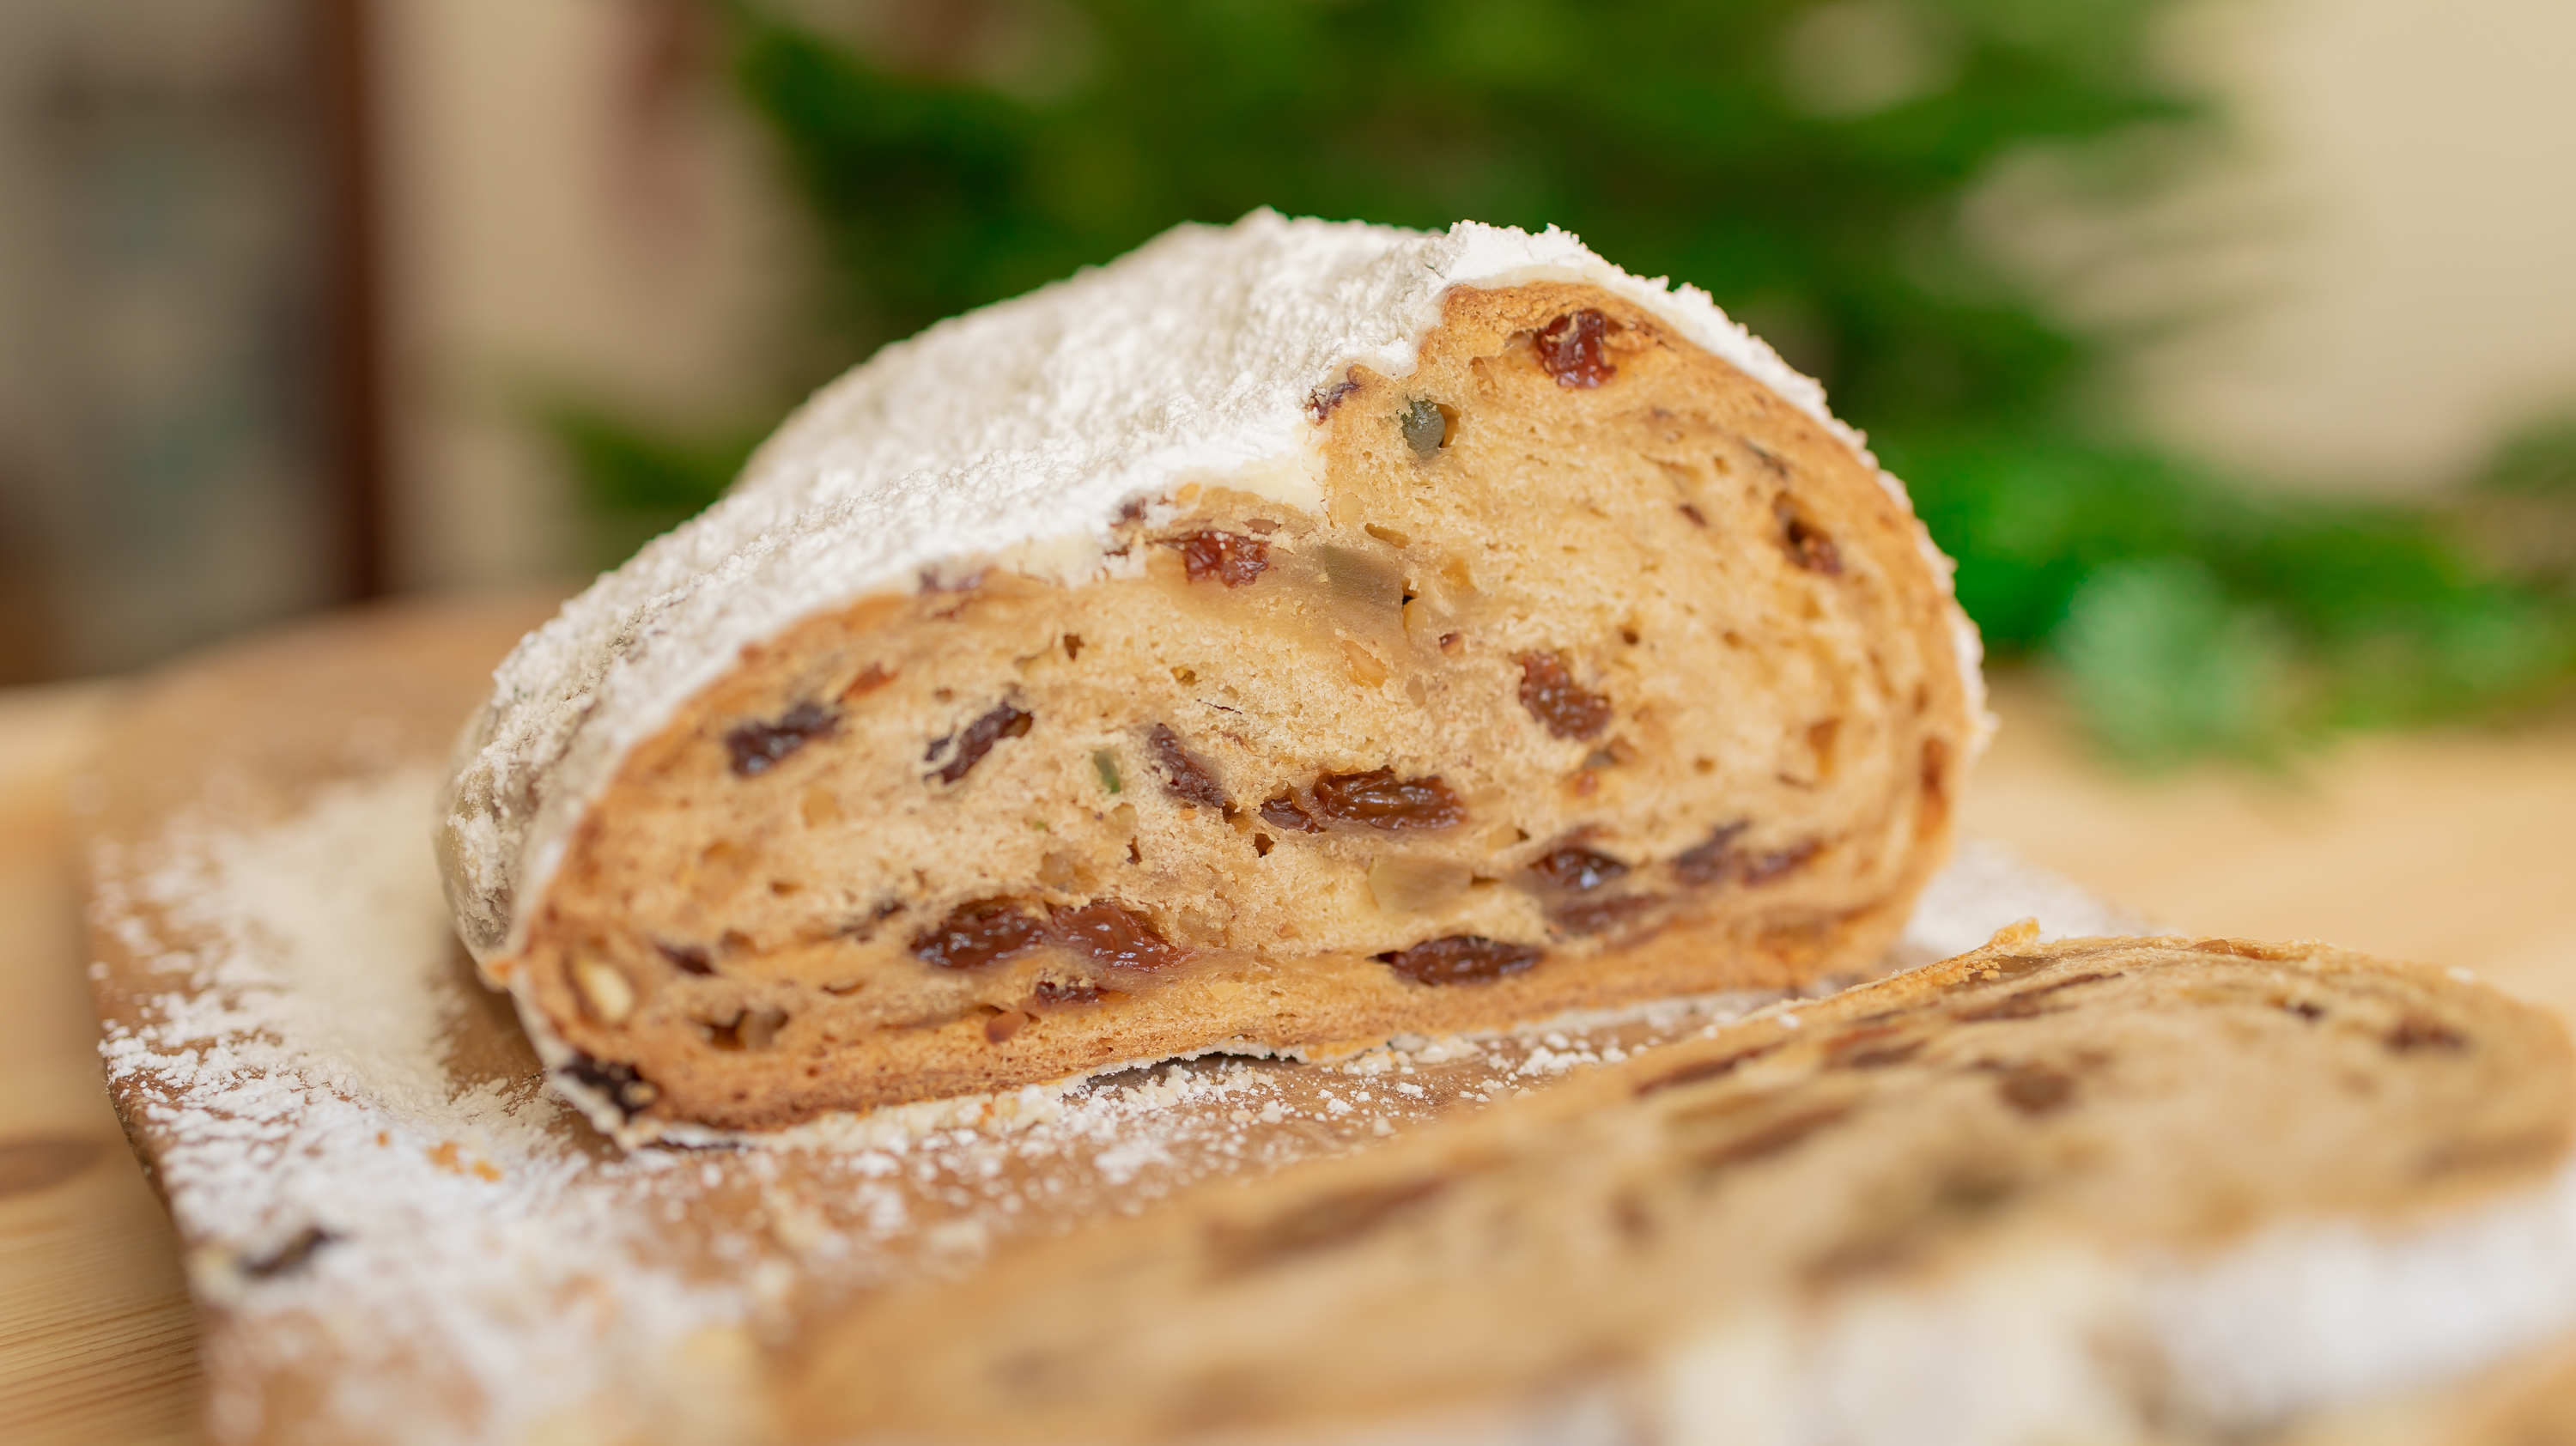
\includegraphics[width=\textwidth]{stollen}
  \caption{A German Christmas stollen made with a stiff starter instead of yeast}
  \label{fig:stollen}
\end{figure}

I then proceeded and bought a cheap low cake flour in my nearby supermarket.
This flour before had caused me massive headaches before. I made a sourdough bread
exactly how I would normally do. I had to reduce the hydration a bit as a low
gluten flour does not soak up as much water. Then I replaced the starter with
the stiff starter. The dough felt amazing and was suddenly able to withstand a
much longer fermentation period. The bread had great oven spring and tasted
very mild. I am still yet to find a proper explanation why the yeast part of
the dough is more active. Maybe it is not. It could also be that the bacteria
is inhibited by the lack of water.

When making the stiff sourdough starter, start by using around 50 percent
water. If you are using a whole wheat flour, or a strong flour consider going
up to 60 percent. All the ingredients should mix together very well. There
should be no crumbly flour left. This is a common mistake I have seen when
people tried to make the stiff starter. Yes it should be dry, but not to a
point where it is a brick of cement. If you have ever made a pasta dough, this
dough should exactly feel the same.

To evaluate whether your stiff starter is ready, look for a dome. Also look for
pockets of air on the sides of your container. Use your nose to smell the
starter. It should have a mild smell. It also tends to smell much more
alcoholic than the other starters.

When using a stiff starter, use around 1 to 20 percent depending on the ripeness of
your starter. In summer I typically use around 10 percent and in winter
around 20 percent. This way you can also control the fermentation speed.
Mixing the starter can be a little bit annoying as it hardly homogenizes with
the rest of the dough. In this case you can try to dissolve the starter in the
water you are about to use for your dough. This will make mixing a lot easier.


\section{Lievito madre or pasta madre}

The lievito madre, also known as pasta madre, belongs to the same category as
the stiff sourdough starter. After conducting hours of research, I could not
find a difference in pasta madre and lievito madre. Both terms seem to be
used interchangeably in literature.

In many recipes this starter is made directly
from dried or fresh fruits. You can also make a starter from leaves from your
garden. As described before, the wild yeast and bacteria consume the glucose
from the plants' leaves. All the options work. When making a starter directly
from dried fruits, you sometimes lack the bacterial part of the fermentation.
The acidity is very important in order to clean your starter from possible
pathogens. If you decide to make your starter from fruits, make sure it also
acidifies properly when making a dough. A tool such as a pH meter can be of
optimal help. Generally, the lower the pH, the higher the acidity. The acidity
should be below 4.2 to know that your starter produces sufficient acidity.

Some bakers cleanse the lievito madre in a bath of water. This is supposed to
remove excess acidity. In my own experiments I have not been able to confirm
this methodology. The acidity remains the same. The only reason this could
make sense is if you also tried to boost anaerobic microorganisms. However, then the
starter would need to remain in this environment for quite some time and not just
a few hours.

Baking with sourdough is simple. It's just flour and water. When seeing a recipe
from an experienced baker you wonder, Wait, that's it? There is nothing more
to it? I feel that this might be the reason why some bakers have such complicated
feeding procedures. They resort to several feedings per day at a certain given ratio.
This makes the baker feel a little more elitist. Of course over time as
more and more people follow this procedure, it becomes a self fulfilling prophecy.
The more experienced you become, the higher the chances are that a bogus starter
feeding guide will reward you with beautiful results. The reason however is
not in the starter routine. The reason is that you understand the fermentation better
and become better at reading the signs of your dough.

If I had to choose one starter type I would go for the stiff starter. In many cases
it will provide you with consistently great results with little effort.
In my experience you can make any yeast-based dough and just replace
the yeast directly with the stiff sourdough starter. You will be able
to achieve even better results with the stiff starter.

Lastly, no matter which starter type you choose, you can control how sour
you want your dough to be. The longer you push the fermentation, the more
acidity is going to be piled up. The only difference is that for a given
volume increase, the stiff starter will produce the least acidity. So for a
volume increase of 100 percent, the liquid starter has produced the most acidity,
followed by the regular starter and then the stiff starter. If you wait long
enough, the stiff starter will have produced the same amount of acidity as the
other starters. But before doing so it will have also produced a lot more \ch{CO2}. If
you like the sour flavor, you have to push your fermentation longer. This also
means you either need to bake in a loaf pan or have a very strong gluten flour
that is able to withstand long fermentation times.


\chapter{Flour types}
In this chapter we will have a closer look at different flour types
and their respective categorization. We will also look a common
ways to distinguish different flours of the same type. This way you can more confidently
shop the right flour that you need.

The most basic flour type is a whole flour. In this case the whole seed has
been ground to smaller pieces. Sometimes depending on what you want to bake
the hearty taste of the bran might not be desired. In this case you can use
whiter flours. With sieves, mills remove larger parts of the hull of the seed.
The seed already contains a pre built germ from the plant waiting to be
activated. The whitest flour you can get is mostly just the starch part of the seed.
Depending on which layers are still present, names are used to describe the
type of flour.

\begin{figure}[!htb]
  \includegraphics[width=\textwidth]{tables/table-flour-types.pdf}
  \label{tab:flour-types-comparison}
  \caption{A comparison of the different wheat flour types}
\end{figure}

In Germany the ash content is used to describe the flours. The lab will burn
100 grams of flour in the oven. Then afterwards the remaining ash is extracted
and measured. Depending on the quantity the flour is categorized. If the flour
is of type 405 then 405 milligrams of ash have remained after burning the
flour. The more hull parts the flour has the more minerals remain. So the
higher the number the closer the flour is to whole flour. The numbers are
slightly different between each grain type. Generally though the higher the
value, the heartier the taste is going to be.

\begin{figure}[htb!]
  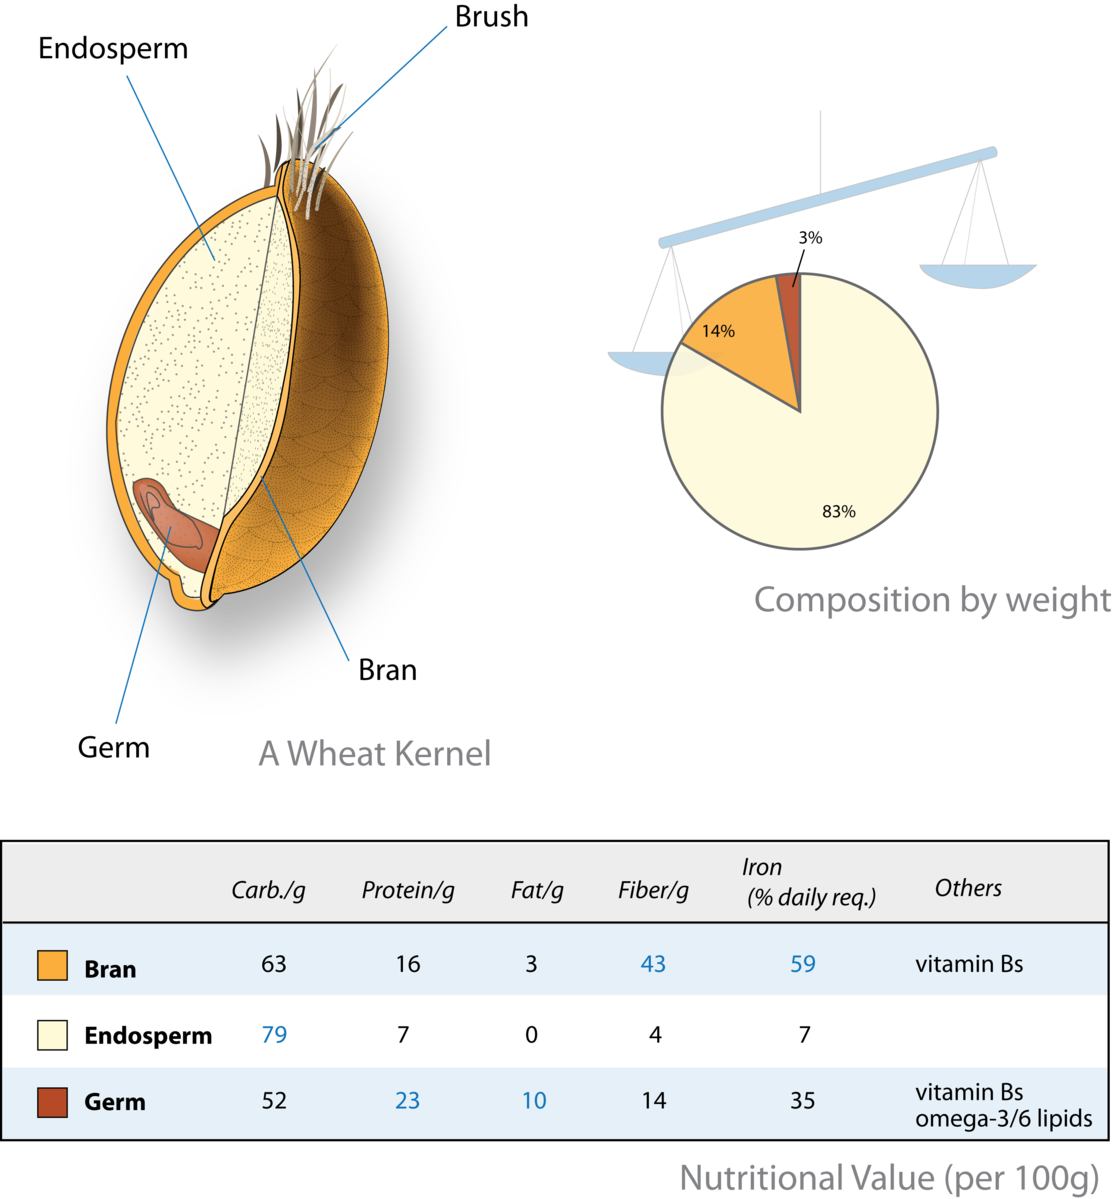
\includegraphics[width=\textwidth]{wheat-kernel-overview}
  \caption{An overview of a wheat kernel together with its content}
  \label{fig:wheat-kernel-overview}
\end{figure}

If you compare different grain types there are grains with high gluten, low gluten
and no gluten. Gluten is what enables bread to have its fluffy consistency.
Without gluten the baked goods wouldn't have the same properties. Managing
gluten makes the whole bread making process more complex as more steps are involved.
A dough without gluten doesn't have to be kneaded. Kneading creates
the gluten bonds. The more you knead the stronger they become. With low
gluten and no gluten flours you only have to mix the ingredients together, making
sure you properly homogenize everything. During the duration of the fermentation
the gluten degrades as the microorganisms metabolize it. When too much gluten
has been converted your dough will no longer have the previously wheat-like described
structure. For no/low gluten flour your main focus is managing acidity. You do not
want the final bread to be too sour. You do not have to worry about the gluten
degradation, removing a huge headache from the equation.

\begin{figure}[!htb]
  \includegraphics[width=\textwidth]{tables/table-grains-bread-making-process.pdf}
  \caption{An overview of different grain types and the steps involved in the respective bread making process}
\end{figure}

As gluten has a special role, the rest of this chapter is dedicated to having a
closer look at different gluten flours and how to distinguish them. Spelt
also contains significant amounts of gluten so the same characteristics hold
true.

Several recipes call for wheat bread flour. Bread flour can refer to different types
of flour. It could be a T405 or a T550 in Germany. This is very often
wrongfully classified. The term  \textit{strong or bread} flour in this case
refers to the properties of the flour. A bread flour is considered to have a
higher number of protein and thus gluten. This flour is excellent when you
want to make a sourdough bread as your dough allows for a longer leavening
period. As described earlier, the gluten is consumed by your microorganisms.
The more gluten you have the longer your dough keeps its integrity. If you wanted
to make a cake you might want to use a flour with less gluten. The gluten binding
properties might not be desirable since the final cake could have a chewy texture.

In conclusion not every T405, T45 or T00 flour is the same. Depending on the properties
of plant they have different properties. For that reason some countries like
Germany have introduced additional scales to evaluate the quality of the
wheat. The category \textbf{A} refers to good quality wheat that can be blended
with poorer qualities to improve the flour. The category \textbf{B} refers to
average wheat that can be used to create different baked goods. Category \textbf{C}
is used for wheat that has poor baking qualities. This could happen for instance
if the wheat already started to sprout and thus lost some of its desirable
baking properties. This type of wheat is typically used as animal feed or
as fermentable biomass for generators. Category \textbf{E} refers to \textit{Elite} wheat. It's
the highest quality of wheat. This kind of wheat can be harvested when the
wheat has grown under optimal conditions. You can compare this to a winery
that uses only the best grapes to make a reserve wine. Unfortunately, this is normally never printed
on the packaging of the flour that you buy. You can look out for the protein
value as a possible indicator. However large mills blend flours together to
maintain quality throughout the years. Blended flour is also not listed on
the packaging. It might be that bakeries extract gluten from some flour and
then mix it in order to create better baking flours.

In Italy the so called
\textbf{W-value} has been introduced to show better how the flour will behave.
A dough is made and then the resistance of this dough to kneading is measured.
The more gluten a flour has the more elastic the dough is and the more it will
resist kneading. A higher W flour will have a higher gluten content and allow for a longer
fermentation period. But at the same time it is also harder for the microbes to
inflate the dough as there is more balloon material. To make an excellent fermented
product out of a high W flour you will need to have a long fermentation period.
The long fermentation period also means that your microbes will enrich
your dough with more flavor.

\begin{figure}[!htb]
  \includegraphics[width=\textwidth]{tables/table-overview-w-values.pdf}
  \caption{An overview of different levels of W values and the respective hydrations and fermentation times}
  \label{tab:w-value}
\end{figure}

Generally, when aiming to
bake free standing sourdough bread aim for a higher protein content. If the
gluten value is relatively low your bread will collapse faster. Baking bread
is still possible, but it might be easier to use tools such as a loaf pan, or
to make pan or flat breads.

An additional rarely considered characteristic of good flour is the level of damage to the
starch molecules. This is a common problem when you are trying to mill your own wheat flours at
home. Chances are that your home mill is not able to achieve the same results
a larger mill can. The damaging of the starches is essential to improve the
properties of the dough. You will have a better gelatinization and water
absorption with properly damaged starch \cite{starch+damage+flour}. As more
starch is damaged the surface area increases. This improves how water connects with the flour.
This also provides a larger surface that your microbes can use to attack the molecules 
and start the fermentation process.

I am still
yet to find a good way of milling my own flour at home. Even after trying to
mill the flour 10 times with short breaks I was not able to achieve the same
properties as with commercially milled flour. The doughs I would make felt
good, maybe a bit coarse. Then during baking however the doughs would start to
degas quickly and turn into very flat breads. I have had great success though when
utilizing home milled flour together with a loaf pan or as a pan bread. If you
have found great ways to work with home milled flour please reach out. The potential
of using home milled flours is huge. It would enable even distant communities
to grow their own wheat and be able to produce amazing freshly baked bread.


\chapter{Bread types}
In this chapter you will learn about different bread types
and their advantages and disadvantages.

At the end of this chapter
you can find a very simple flat bread recipe. This is probably
the most accessible, least effort type of bread you can make.
If you are a busy person and/or don't have an oven this might
be exactly the type of bread you should consider.

\begin{table}[htp!]
  \centering
  \resizebox{\textwidth}{!}{%
  \begin{tabular}{|l|l|l|l|}
  \hline
                                   & \textbf{Flat bread} & \textbf{Loaf pan bread} & \textbf{Free standing bread} \\ \hline
  \textbf{Cooking method}          & Fire, pan, barbecue & Oven                    & Oven                         \\ \hline
  \textbf{Working time in minutes} & 3                   & 5                       & 60                           \\ \hline
  \textbf{Flour types}             & All                 & All                     & Gluten flours                \\ \hline
  \textbf{Difficulty}              & Very easy           & Easy                    & Difficult                    \\ \hline
  \textbf{Cost}                    & Low                 & Medium                  & High                         \\ \hline
  \end{tabular}%
  }
  \caption{\label{tab:bread-types-comparison}An overview of different bread types}
  \end{table}

\section{Flat bread}

Flat bread is probably the simplest sourdough bread to make.
To make a flat bread no oven is required, all you need is a stove.

\begin{figure}[!htb]
  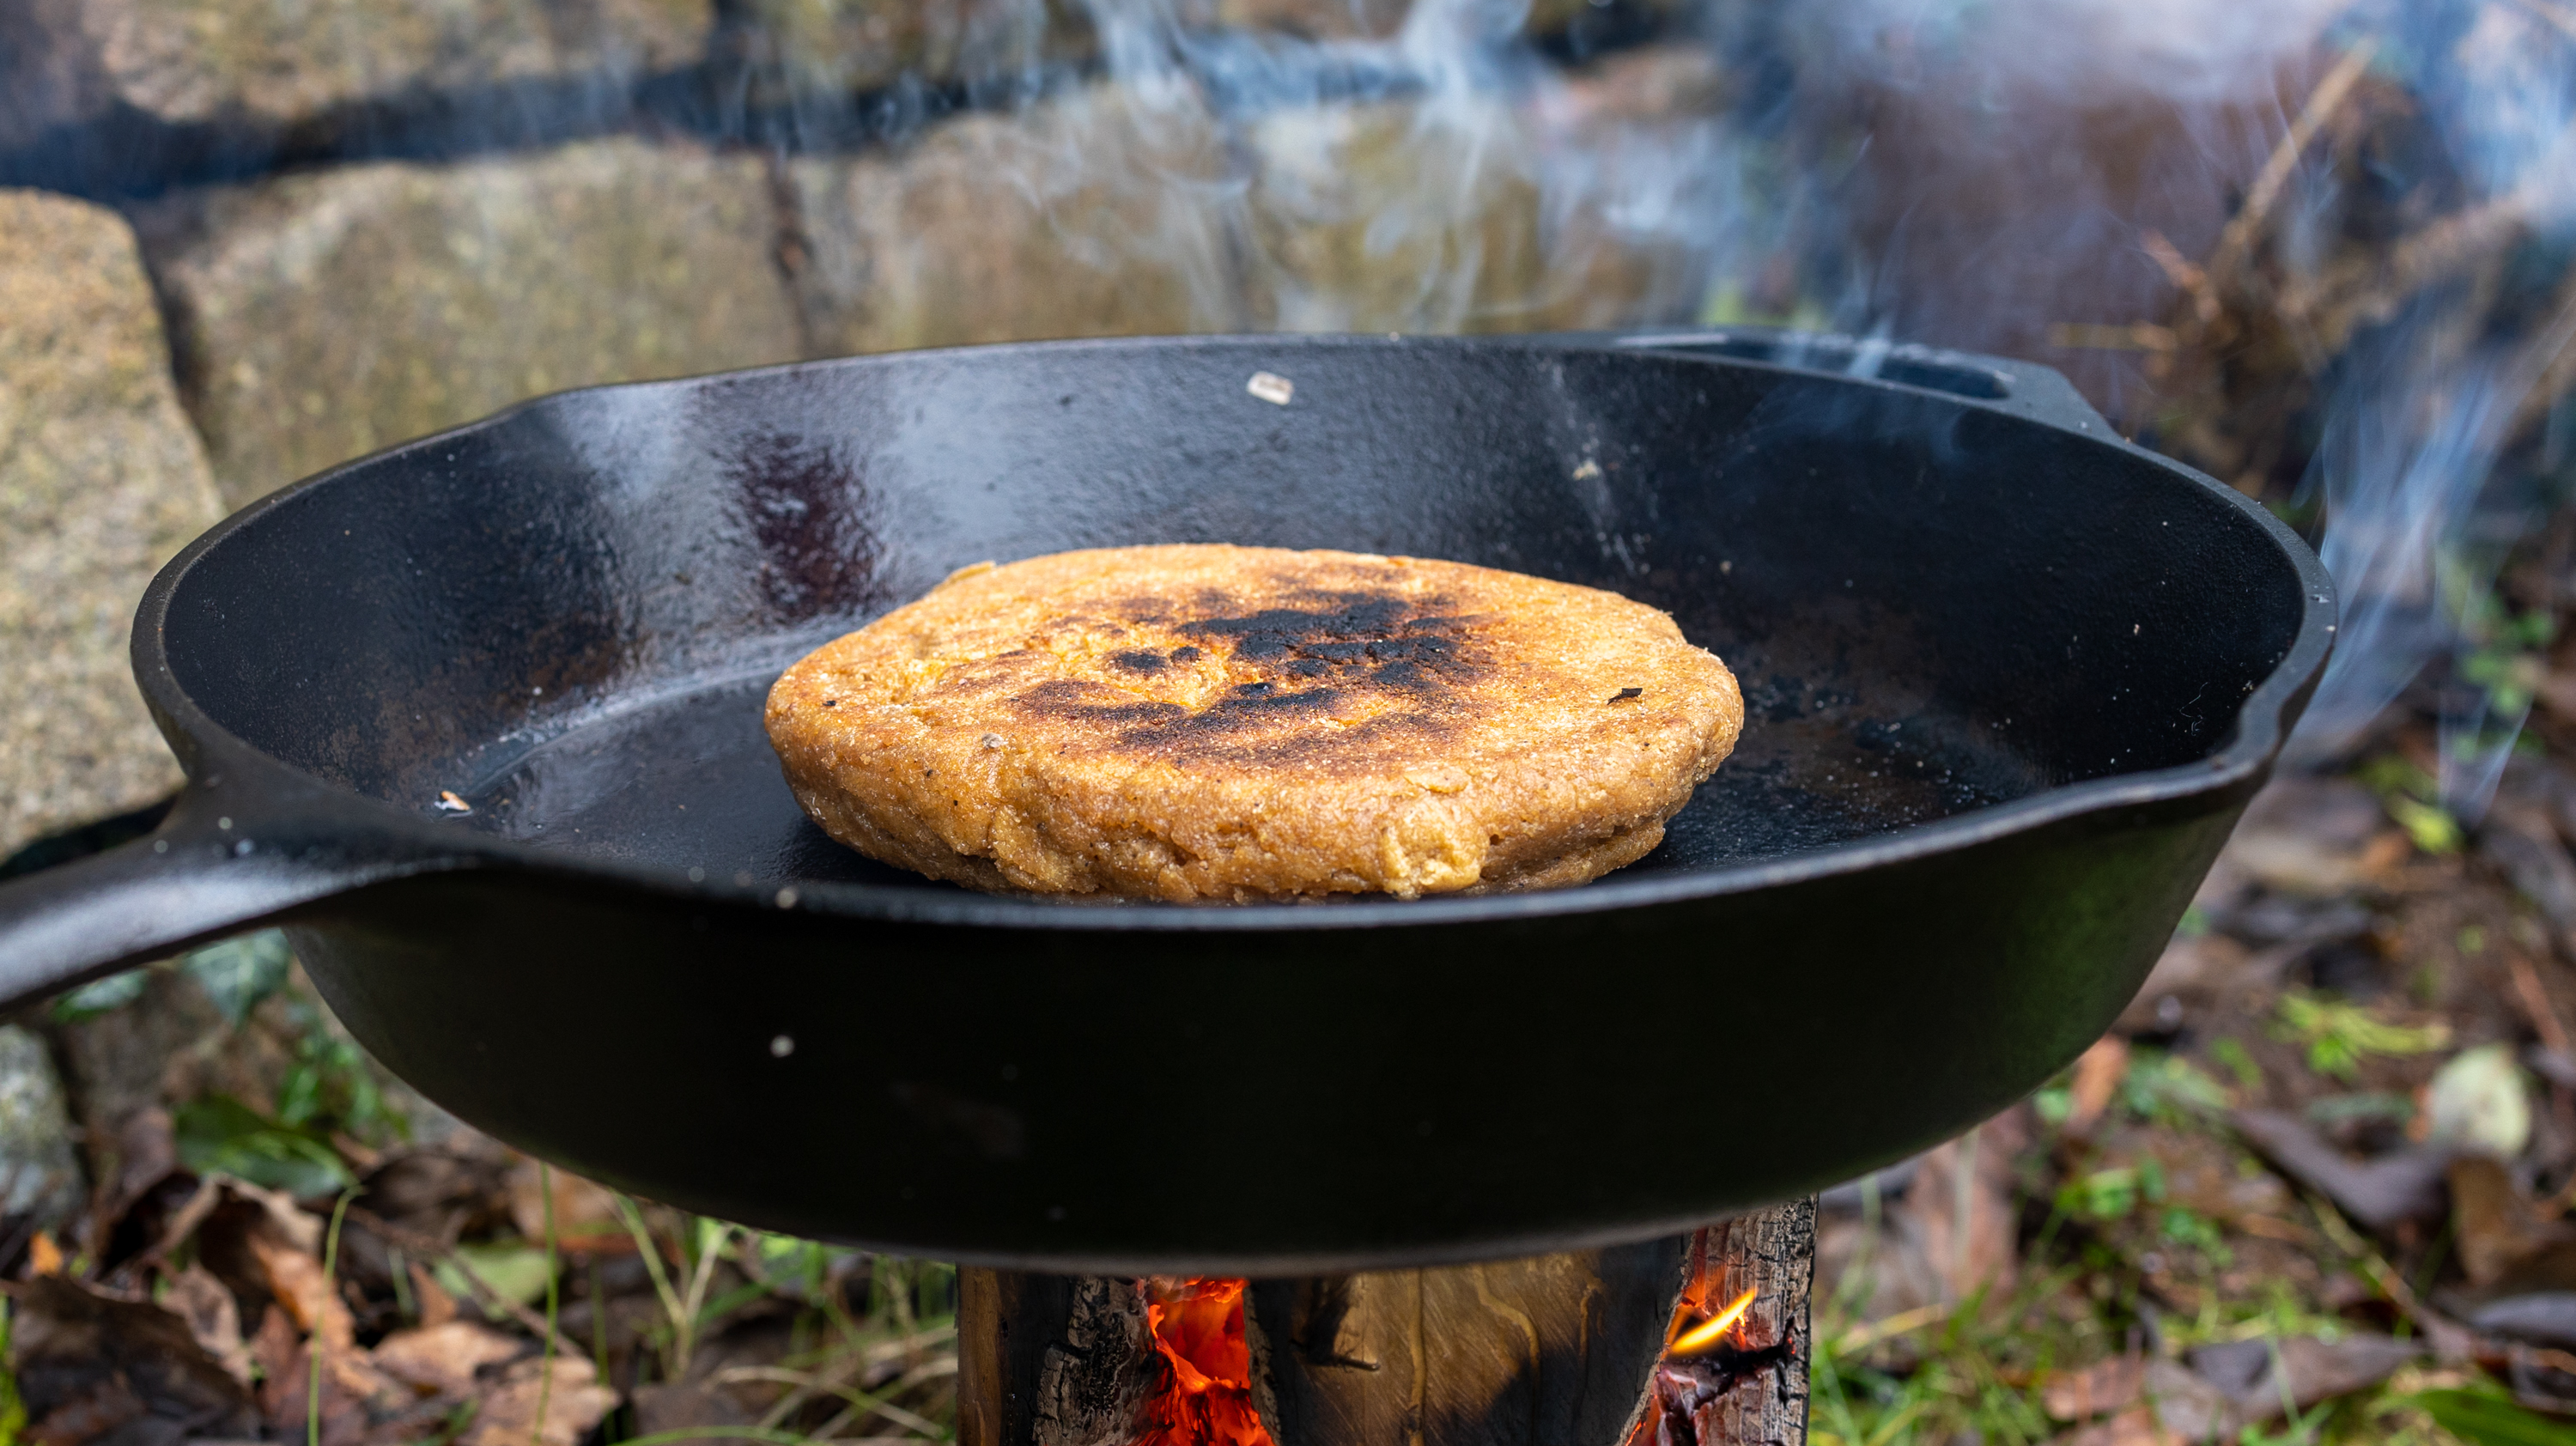
\includegraphics[width=\textwidth]{sourdough-stove}
  \caption{An einkorn flat bread made directly over fire. This
  is part of a video where I was trying to reproduce sourdough
  recipes of our ancestors. I called the recipe "cave bread". Some viewers
  pointed out that probably not all our ancestors lived in caves
  }
\end{figure}

This type of bread is super simple to make as you can skip
a lot of the technique that is normally required. The flat
bread can be made with all kinds of flour. You can even use
flour without gluten such as corn or rice flour to make such
a dough. To make the flat bread a little more fluffy you
can use a little bit of wheat flour. The developing gluten
will trap the gasses. During baking theses gasses will
inflate the dough.

Another trick to improve the texture of the flat bread is to
make a very wet dough. A lot of the water will evaporate
during the baking process and thus make the bread fluffier.

If you go very high in water content you have a pancake
like consistency.

Refer to section \ref{section:flat-bread-recipe} "\nameref{section:flat-bread-recipe}"
to see a full recipe including the process of making such a flat bread.

\section{Loaf pan bread}

Loaf pan bread is made using the help of a special loaf pan
or loaf tin. The edges of the pan provide additional support
for the dough to rise. Making a bread using a loaf pan requires
an oven.

\begin{figure}[!htb]
  \includegraphics[width=\textwidth]{loaf-pan-free-standing.jpg}
  \caption{A free standing bread and a wheat loaf pan bread. Both of them
  received a small incision before baking allowing them to
  better open up}
  \label{fig:free-standing-loaf-pan}
\end{figure}

After mixing the ingredients of your dough you can directly
place the dough inside of the loaf pan. This makes the whole
process simpler as you can skip steps such as shaping the dough.

To make a great loaf pan bread with little work:

1. Mix the ingredients of your dough (gluten free works too)
2. Place in the loaf pan
3. Wait until your dough roughly doubled in size
4. Bake in a non pre-heated oven for around 30-50 minutes

Knowing the exact baking time is sometimes a little challenging
as it might be that the outside of your bread is cooked but
the inside is not yet. The best way is to use a thermometer
and measure the core temperature. At around 92°C (197°F) your
dough is done. I generally bake loaf pan bread at around 200°C (390°F),
which is a little less than my free standing bread which I bake
at 230°C (445°F). That's because it takes a while for the dough
to properly bake inside of the loaf pan. The edges don't heat up
as fast. Then the top part of the dough is properly cooked, while
the inside isn't yet. When baking make sure to use steam
or simply place another equally sized loaf pan on top
of your loaf pan. This way you simulate a dutch oven. The dough's
evaporating moisture will stay inside.

A good trick to make excellent loaf pan bread is to make a very
sticky dough. You can opt for a hydration of 90-100 percent, almost
resembling a default sourdough starter. Just like with flat bread
the high humidity helps to make a more airy fluffy crumb. At
the same time the bread will be a bit more chewy when eating. This
type of bread made with rye is my family's favorite style of bread.
The hearty rye flavor paired with the sticky consistency really
makes an excellent sandwich bread.

To improve structure you can also consider to use around 50 percent
wheat flour in your mix. The gluten network will develop as your
dough ferments and allow for more gas to be trapped in the dough.

A common problem you will face when making a loaf pan bread is
the dough sticking to the pan. Generously use an oil to grease
your pan. A non-stick vegetable oil spray can also do wonders.
Don't clean your loaf pans with soap. Just use a kitchen towel
to clean them. With each bake a better patina forms making your
pan more and more stick resistant.

What's amazing about this type of bread is that it works
with every flour. Overall time to work the dough is probably
less than 5 minutes, making it very easy to integrate
into your daily routine. Furthermore loaf pans use the space
in your oven very efficiently. Using the pans I can
easily bake 5 loafs at the same time in my home oven.
Normally I would need multiple baking sessions for
free standing loaves.

\section{Free standing bread}

A free standing loaf is baked as whole without support
in your oven. To make a free standing loaf more steps
and tools are required.

\begin{figure}[!htb]
  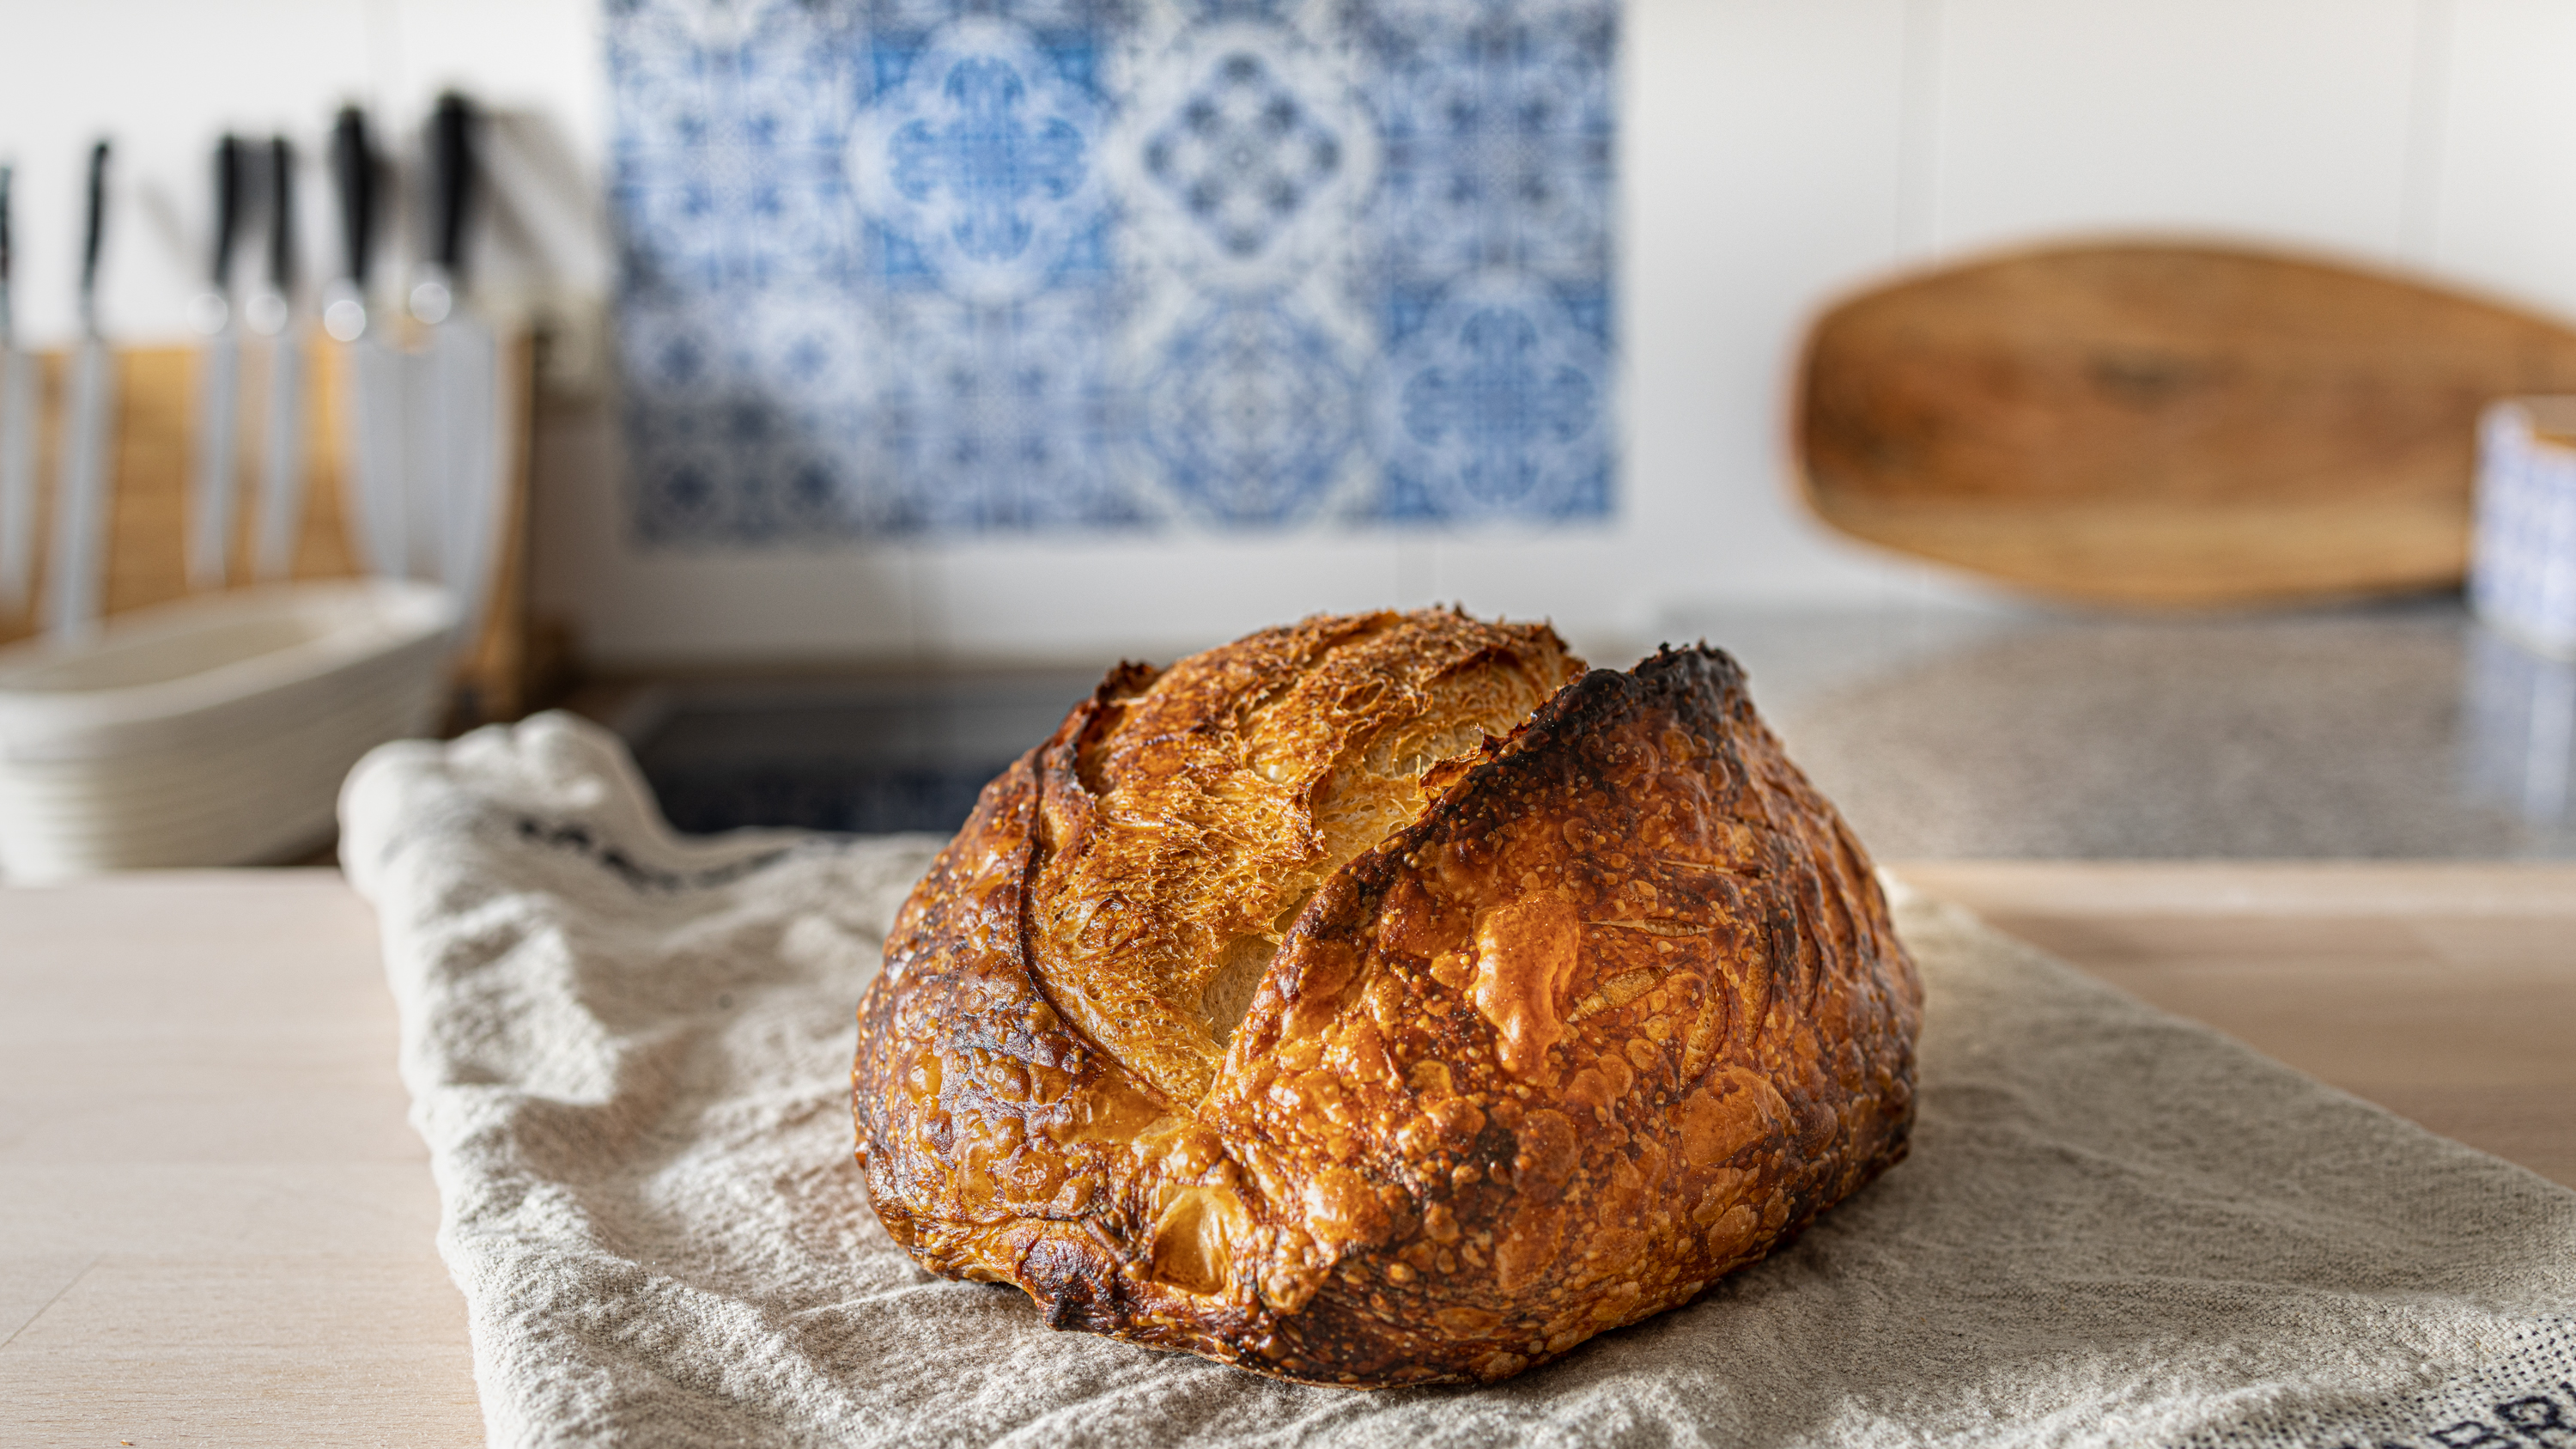
\includegraphics[width=1.0\textwidth]{free-standing-loaf.jpg}
  \centering
  \caption{A free standing sourdough bread. Note the incision known as "ear" and the oven spring clearly
  distinguishing this type of bread from the flat and loaf pan bread}
\end{figure}

Normally you mix your dough. When using wheat you make sure
that you mix enough to develop a gluten network.
You allow the dough to reach
a certain size increase during the fermentation. Afterwards you divide and preshape
the dough into the desired visual shape that you like.
Each shape requires a different technique. Sometimes achieving
exactly that shape can be more challenging. Making a baguette
for instance requires you to perform more steps. Mastering this
technique takes several attempts.

Once the dough is shaped it is proofed again for a certain
period of time. Once the dough is ready a sharp tool such
as a razor blade is used to make an incision into the dough.
This helps the dough to better open up during the baking process.

All these steps require practice. Each of them has to be
performed in a perfect manner, not allowing mistakes.
But after baking you will be rewarded with a beautiful bread
rewarding you with great taste and consistency.

There is a fully dedicated recipe and tutorial
for this type of bread in the "\nameref{chapter:wheat-sourdough}" chapter.

\section{Simple flat bread recipe}
\label{section:flat-bread-recipe}

If you are just getting started making a flat bread is the
easiest way to start making great bread at home. With just a
few steps you can stop buying bread forever. This works with
every flour, including gluten free options.

\begin{figure}[htb!]
  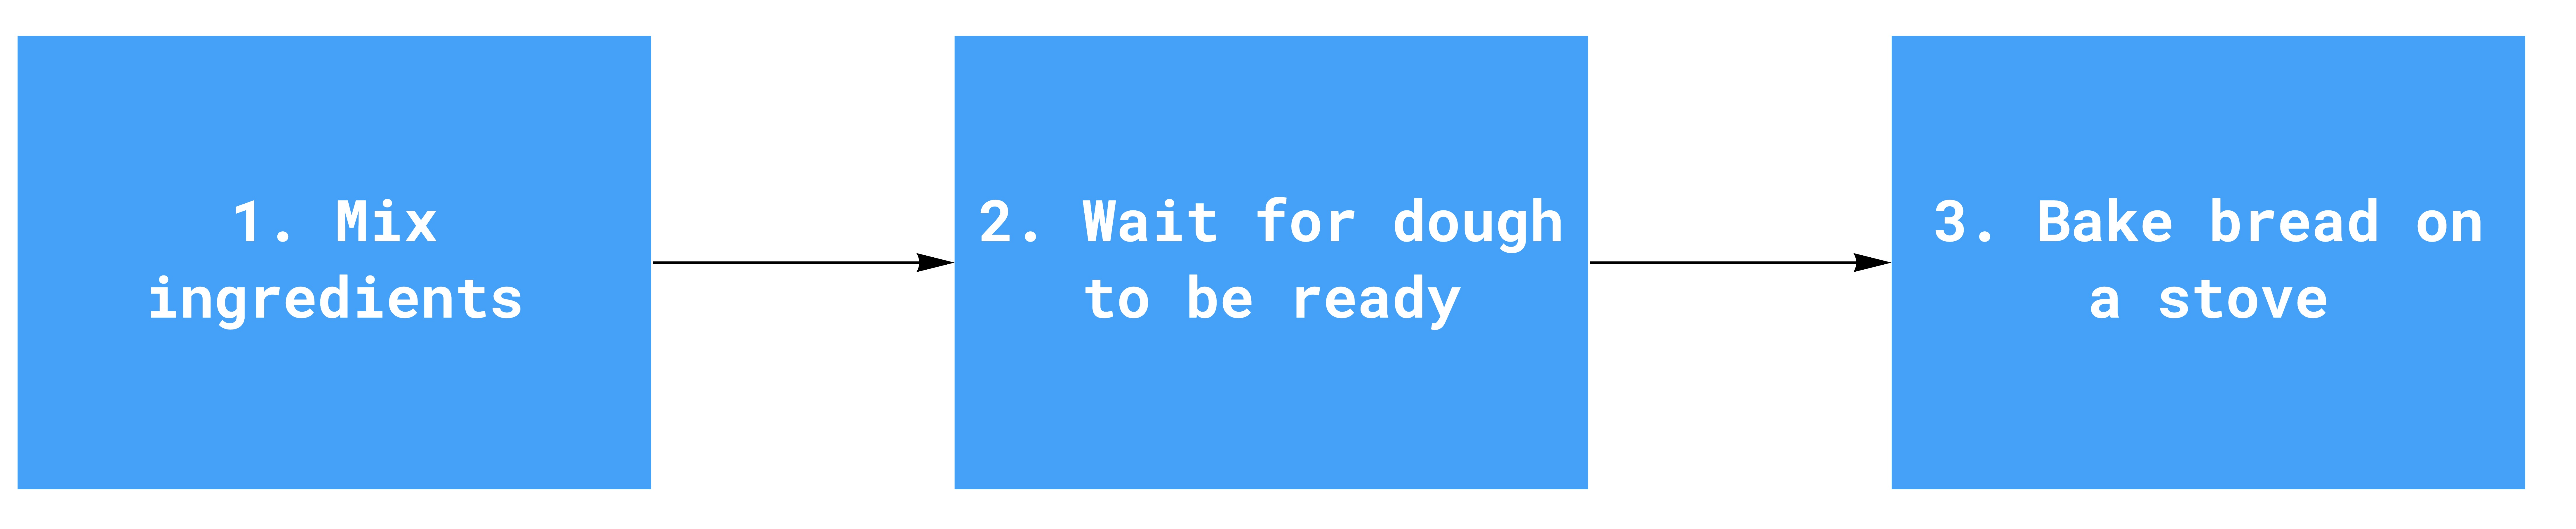
\includegraphics[width=1.0\textwidth]{flat-bread-process}
  \centering
  \caption{The simple process of making a flat bread}
\end{figure}

This is my goto recipe that I use to make bread whenever
I have little time or when I am abroad. You can choose
between two options. 1) A flat bread similar to a roti or naan bread
or 2) sourdough pancakes.

\begin{table}[htb!]
  \centering
  \resizebox{\textwidth}{!}{%
  \begin{tabular}{|l|l|l|}
  \hline
                             & \textbf{Flat breads} & \textbf{Pancakes}                        \\ \hline
  \textbf{Flour}             & 100g                               & 100g                       \\ \hline
  \textbf{Water}             & 100g (100\%)                       & 300g (300\%)               \\ \hline
  \textbf{Sourdough starter} & 5-20g (5-20\%)                     & 5-20g (5-20\%)             \\ \hline
  \textbf{Salt}              & 2g (2\%)                           & 2g (2\%)                   \\ \hline
  \textbf{When bake?}        & Dough increased 50 percent in size & Bubbles visible on surface \\ \hline
  \end{tabular}%
  }
  \caption{\label{tab:flat-bread-ingredients}Flat breads or pancakes recipe for 1 person. Multiply the ingredients
  to increase portion size. Refer to the section \ref{section:bakers-math} "\nameref{section:bakers-math}" to learn how
  to understand and use the percentages properly.} 
\end{table}

To get started prepare your sourdough starter. If it has not been using for a very
long time consider giving it another feeding. To do so simply take 1g of your
existing sourdough starter and feed it with 5 grams of flour and 5 grams of water.
If you do this in the morning your sourdough starter is ready in the evening. The
warmer it is the faster this process goes. If it is very cold where you live, consider
using warm water.

\begin{figure}[htb!]
  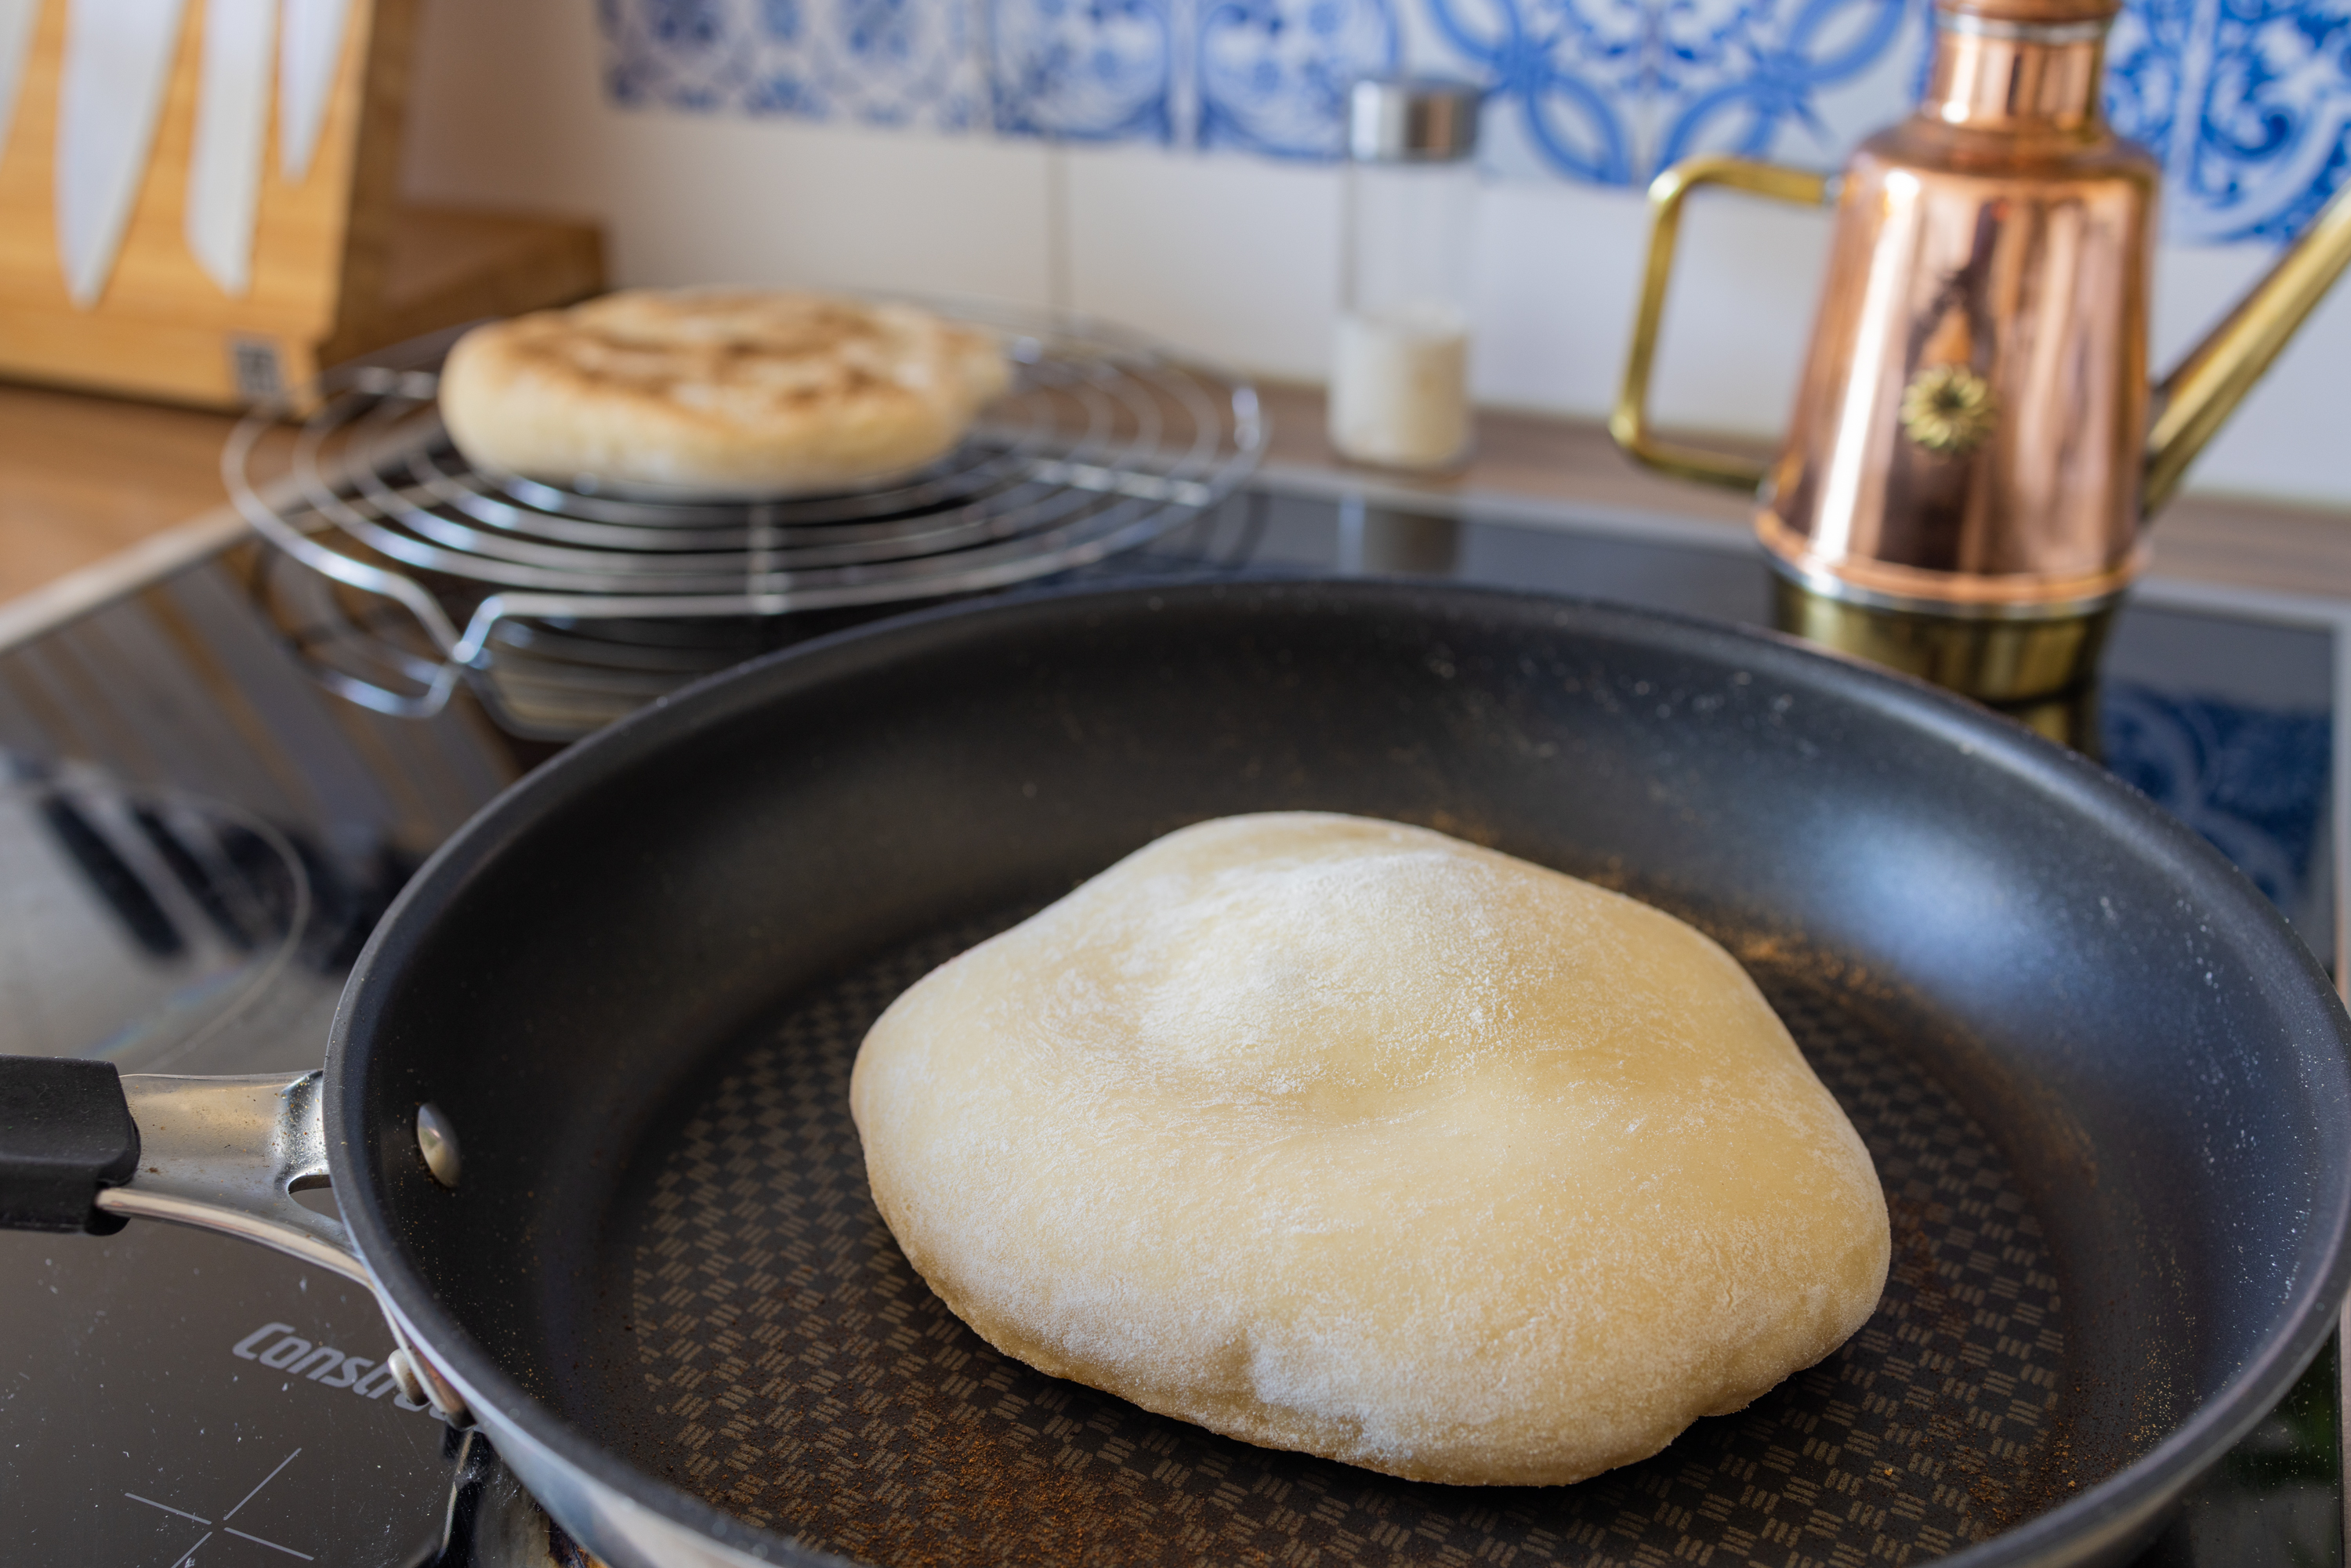
\includegraphics[width=1.0\textwidth]{flat-bread-wheat}
  \centering
  \caption{A flat bread made with purely wheat flour. The dough is drier
  at around 60 percent hydration.  The drier dough is a little harder
  to mix. As wheat contains more gluten the dough puffs up during
  the baking process}
\end{figure}

This way you should have around 11g of sourdough ready in the evening. You will have
the perfect quantity to make a dough for a single person. In case you want to make more
bread simply multiply the quantities shown in table \ref*{tab:flat-bread-ingredients}.

Then in the evening simply mix the ingredients as shown in the table. Your dough
is going to be ready in the morning. It's typically ready after 6-12 hours. If
you use more sourdough starter it will be ready faster. If you use less it takes
longer. Try to aim for a fermentation time of 8-12 hours. If you use
your dough too soon the flavour might not be as good. If you use it later
your dough might be a little more on the sourer side. The best option is to experiment
and see what you personally like the most.

After mixing the ingredients together cover the container in which
you made the dough. This prevents the dough from drying out and makes
sure no fruit flies get access. A transparent container will be helpful
when getting stared. You can better observe the dough and see when
it is ready.

\begin{figure}[htb!]
  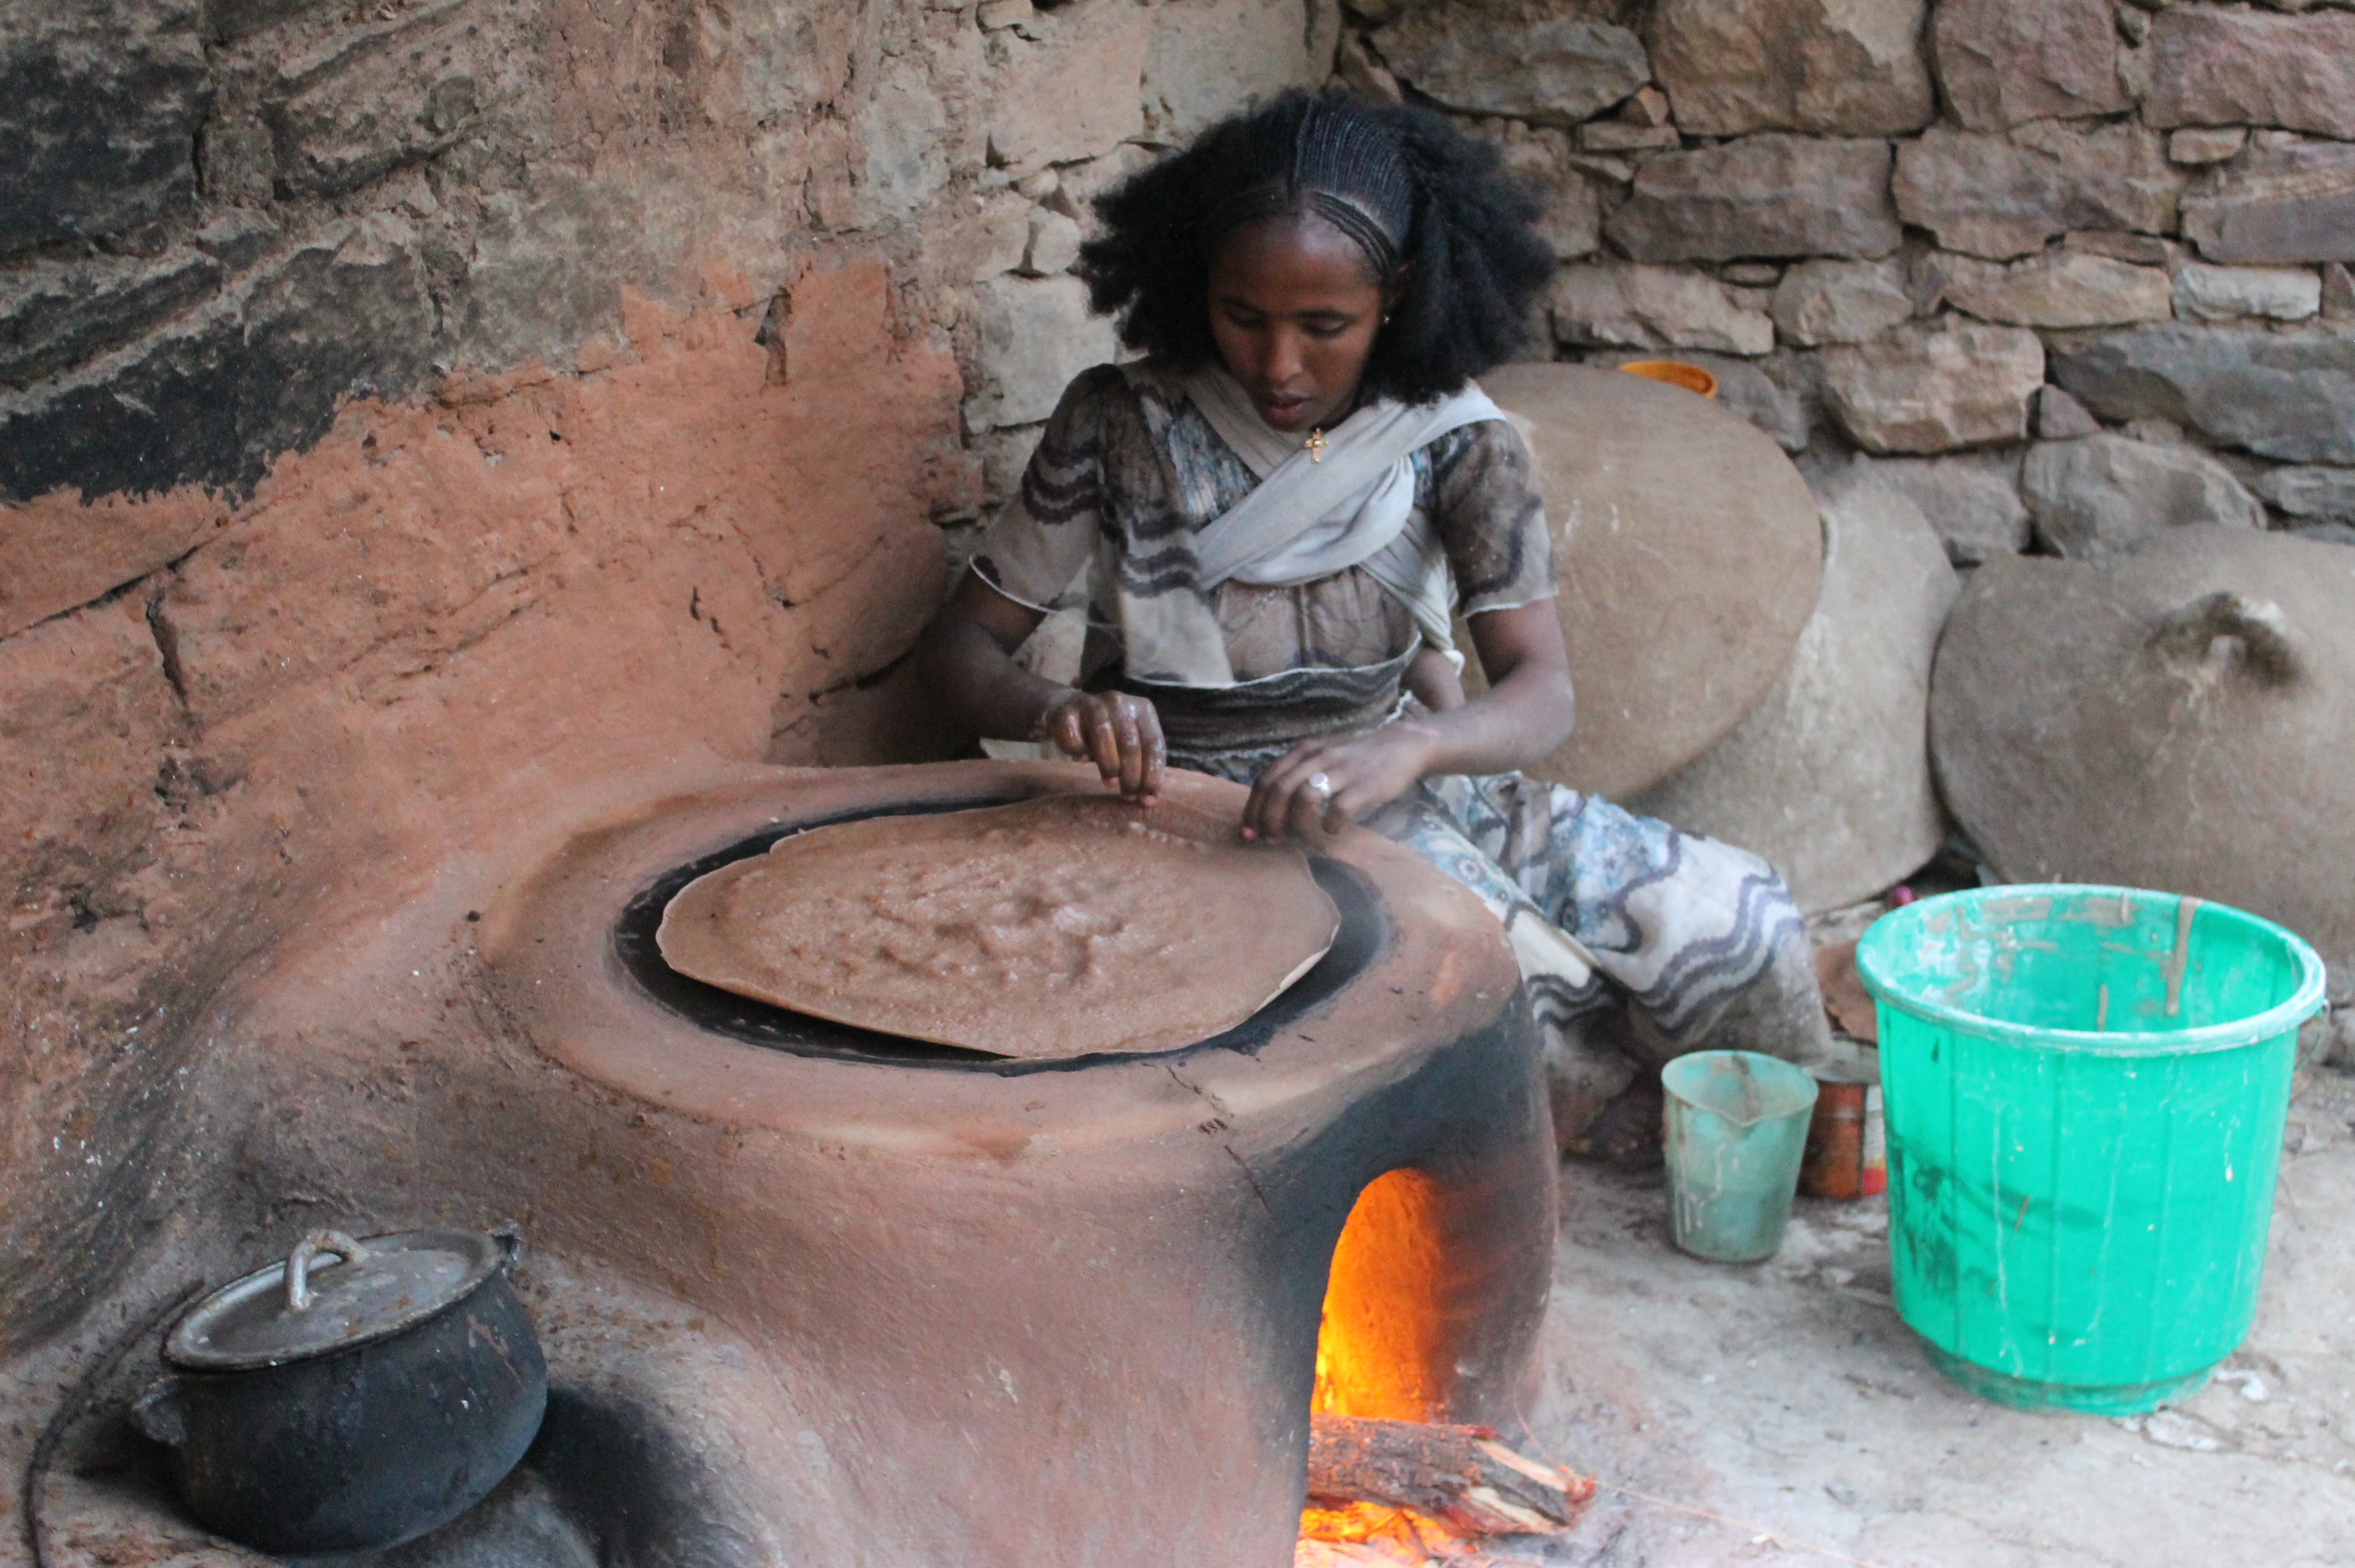
\includegraphics[width=1.0\textwidth]{ethiopian-woman-checking-bread.jpeg}
  \centering
  \caption{An ethiopian woman baking an "injera" made using teff flour. 
  The image has been provided by Charliefleurene via Wikipedia}
\end{figure}

If you used the flat bread option with less water look at a size increase
of your dough. The dough should have increased at least 50 percent in size.
Also look out for bubbles bubbles on the edges of your container.
When going the pancake route look out for bubbles on the surface of your dough.
In both cases use your nose to check the scent of your dough. Depending
on your sourdough starter's microbiome your dough will have 
dairy, fruity alcoholic notes or vinegary acetic notes. Relying
on the smell of your dough is best way to judge whether your
dough is ready or not. Timings are not reliable as they
depend on your starter and temperature. If your dough
is ready too soon you can now move it directly to the fridge to bake
it at a later more convenient time. The low temperature will halt the fermentation
process\footnote{There are some exceptions. In some rare cases your starter
might also work at lower temperatures. You might have cultivated low temperature appreciating
microbes. Regardless though the fermentation
is always slower the colder it gets. A fridge really helps to preserve the state
of your dough.}
and your dough is going to be good for several days. The longer you wait the more sour the
bread is going to be. The fridge is a great option in case you wanted to
take the dough with you when visiting friends. People are going
to love you for the freshly baked flat breads or pancakes. If you dare
you can also taste a little bit of your raw uncooked dough. It is likely
going to taste relatively sour. I do this frequently to better evaluate the
state of my doughs.


\begin{figure}[htb!]
  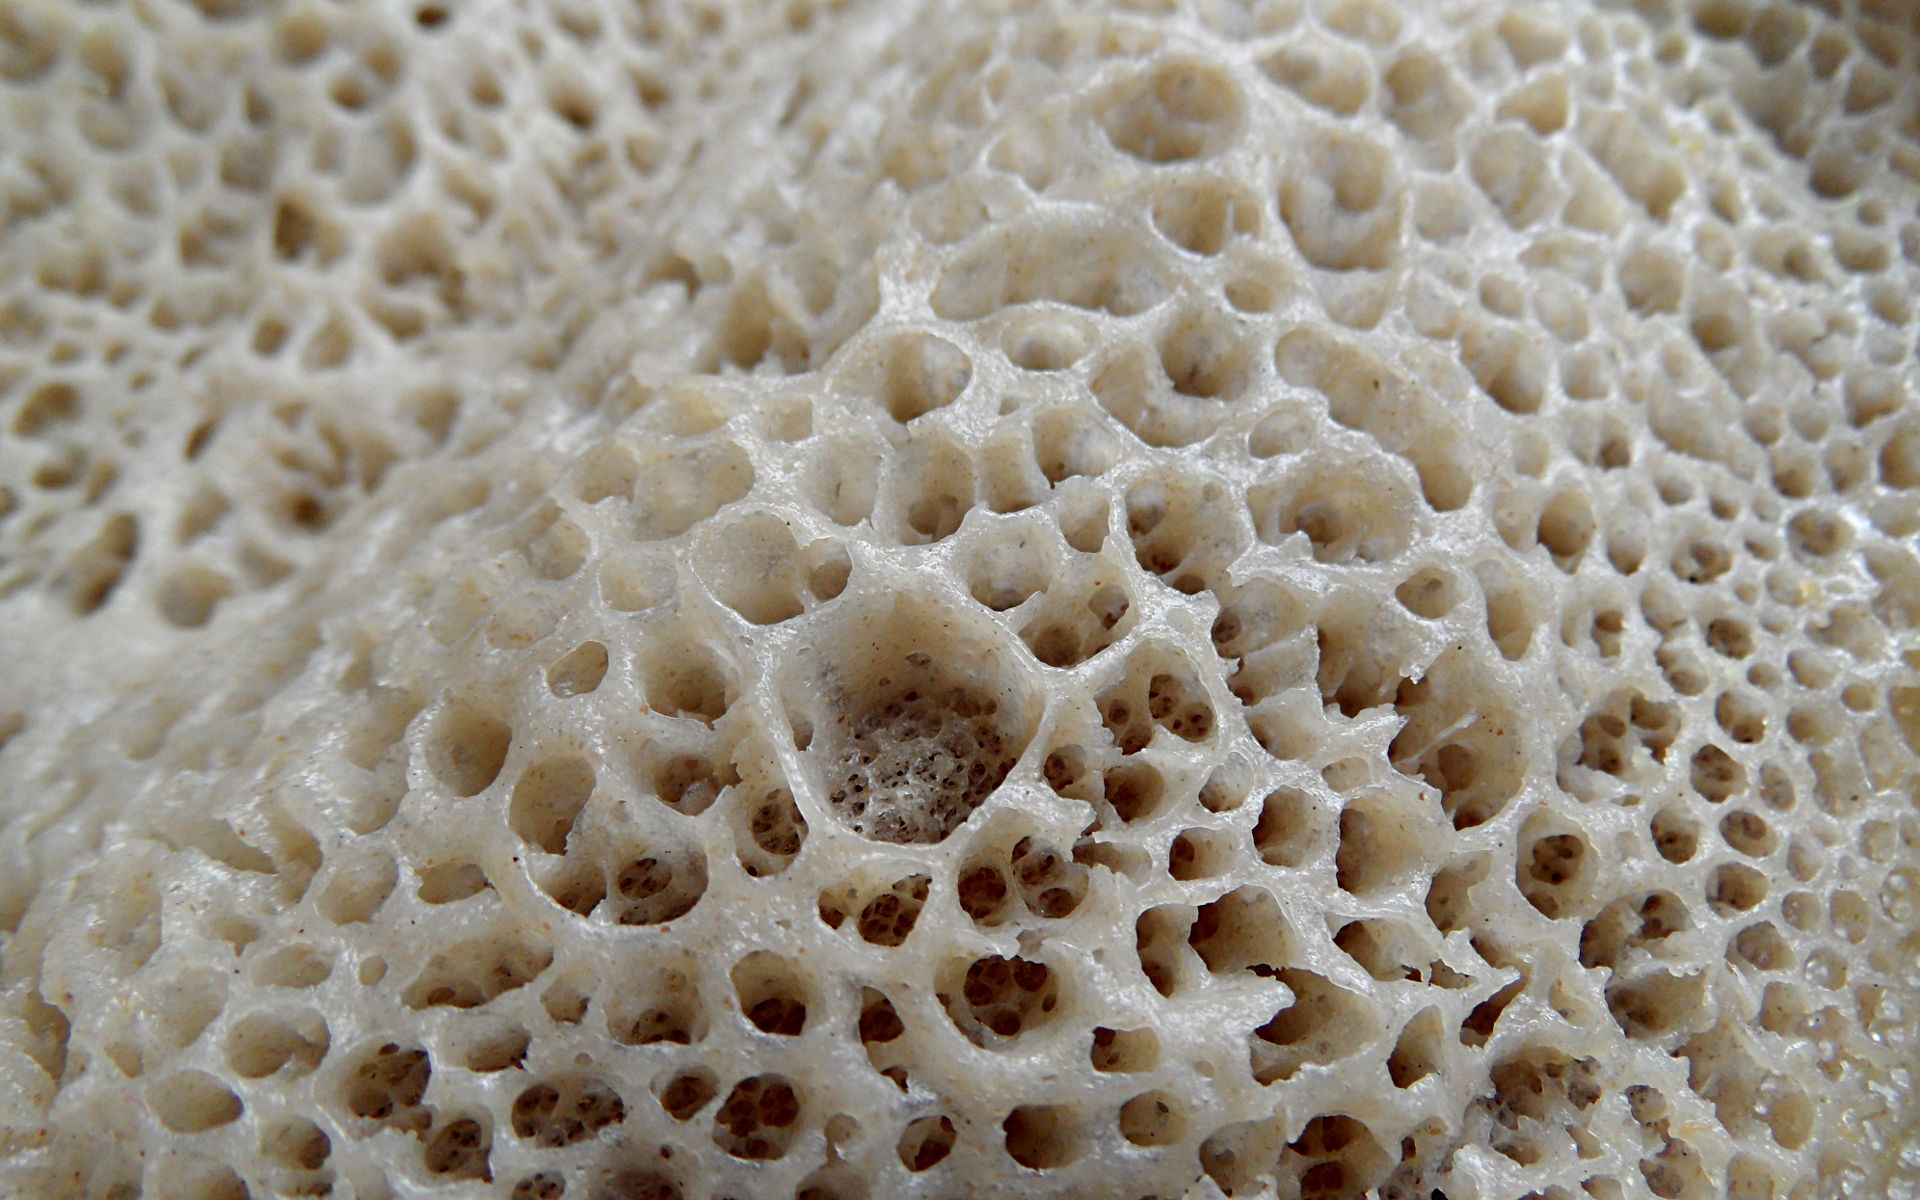
\includegraphics[width=1.0\textwidth]{injera-pancake-texture.jpg}
  \centering
  \caption{A sourdough pancake made with teff flour. The pockets are coming from
  the evaporated water and CO2 created by the microbes.
  The image has been provided by Lukasz Nowak via Wikipedia}
\end{figure}

If you are completely lazy or don't have time, you could also use older sourdough starter
to make the dough directly without any prior starter feedings. Your sourdough starter
is going to regrow inside of your dough. The
final bread might be a bit more on the sour side as the balance of yeast to
bacteria could be a off. In the table I recommended to use around 5 to 20 percent
of sourdough starter based on the flour to make the dough. If you were to follow
this approach just use around 1 percent and make the dough directly.
The dough is probably going to be ready 24 hours later depending on the temperature.

If you wanted to make sweet pan cakes, add some sugar and optional eggs to your dough
now. A good quantity of eggs is around 1 egg per 100 grams of flour.
Stir your dough a little bit and it is ready to be used. You'll 
have delicious sweet savory pancakes, the perfect combination. By
adding the sugar now you make sure that the microbes don't have
enough time to fully ferment it. If you had added the sugar
earlier no sweet flavour would be left 12 hours later.

To bake your dough heat your stove to medium temperature. Add a little bit of
oil to the pan. This helps with heat distribution and ensures even cooking.
With a spatula or a spoon place your dough in the pan. If your dough
was sitting in the fridge bake it directly. There is no need to wait for your
dough to come to room temperature. If you have a lid
place it on your pan. The lid helps to better cook your dough from the top.
The evaporating water will circulate and heat up the dough's surface. When
making a flat bread make the dough around 1cm thick. When using the pancake
option opt for around 0.1-0.5cm depending on what you like.

\begin{figure}[htb!]
  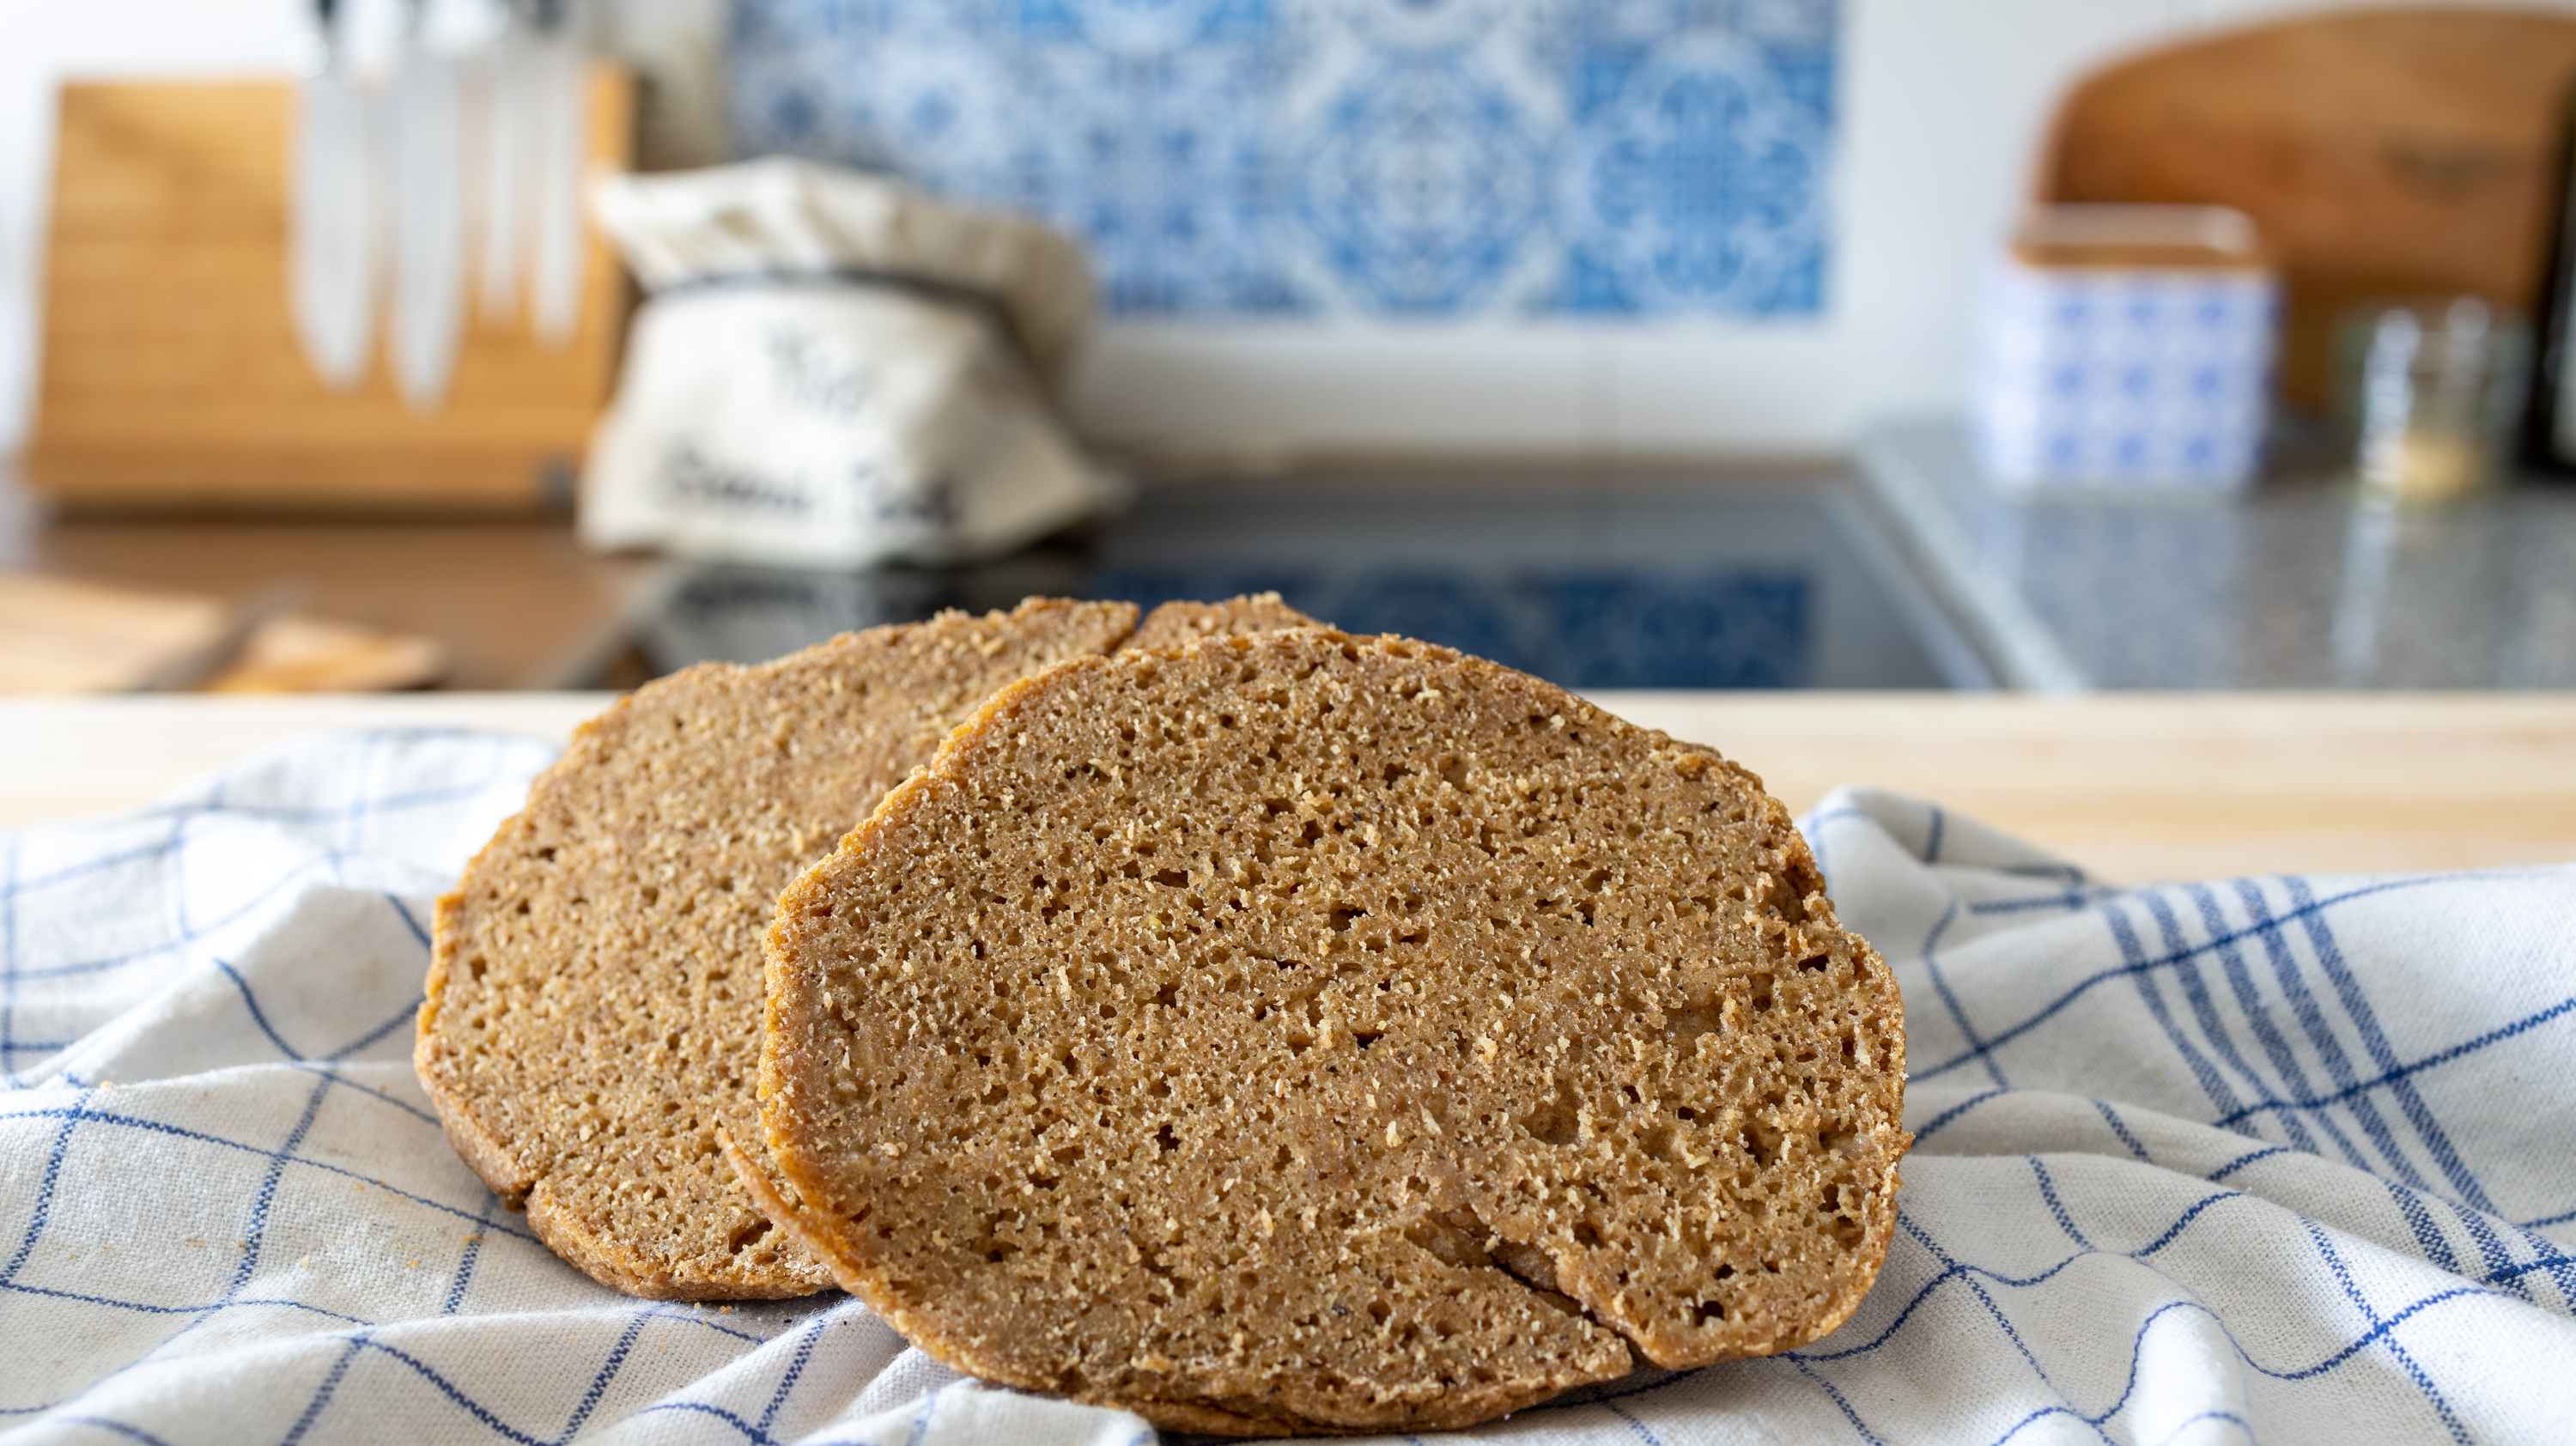
\includegraphics[width=1.0\textwidth]{einkorn-crumb.jpg}
  \centering
  \caption{The crumb of a flat bread made with einkorn as flour. Einkorn
  is very low in gluten and thus does not trap as much CO2 as a wheat based
  though. To make the dough fluffier use more water or consider adding
  more wheat to the mix of your dough.}
\end{figure}

After 2-4 minutes flip over the pancake or flat bread. Bake it for the same
time from the other side. Depending on what you like, you can wait a little
longer to allow the breads to become a bit charred.  The longer you
bake your breads the more of the acidity is going to evaporate. If your
dough is a bit more on the sour side you can use this trick to balance
out the acidity. This really depends on which flavor you are looking for.

When making a flat bread I recommend to wrap the baked flat breads
in a kitchen towel. This way more of the evaporating humidity
stays inside of your breads. This makes sure your flat breads stay
nice and fluffy for a longer period after the bake. A similar option is
used when making corn tortillas.

You can safely store the baked flat breads or pan cakes in your fridge
for weeks. When storing make sure to store them in an airtight plastic bag so that
they do not dry out.

Keep a little bit of your unbaked dough. You can use it to make the next
batch of bread or pancakes for the next day. If you want to bake a few days later, add
a little bit of water and flour and store this mixture in your fridge
for as long as you like.\footnote{The starter will stay good for months. If you are out
for longer consider drying a little bit of your sourdough starter.}

\chapter{Wheat sourdough}
\label{chapter:wheat-sourdough}

\section{The process}
\section{Readying your starter}
\section{Ingredients}
\section{Hydration}
\section{Autolyse}
\section{Fermentolyse}
\section{Dough strength}
\section{Controlling fermentation}
\section{Optional Preshaping}
\section{Shaping}
\section{Proofing}
\section{Scoring}

\chapter{Non wheat bread basics}
\section{Ingredients}
\section{Managing acidity}
\section{To shape or not to shape}
\section{Proofing}

\chapter{Baking}
Baking refers to the part of the process where you are loading
your dough into the oven. This is typically done after your
dough has gone through the bulk fermentation and proofing stage.


\begin{figure}[!htb]
  \begin{tikzpicture}[node distance = 3cm, auto]
    \node [block] (heat_oven) {\footnotesize Heat oven to 230°C (446°F) for 30 minutes};
    \node [block, right of=heat_oven, node distance=3cm] (score_dough) {\footnotesize Score your dough};
    \node [decision, right of=score_dough, node distance=4cm] (decide_steam) {\footnotesize Choose your steaming method};
    \node [block, below of=heat_oven, node distance=4cm] (inverted_tray_method) {\footnotesize Inverted tray method};
    \node [block, right of=inverted_tray_method, node distance=3cm] (dutch_oven) {\footnotesize Dutch oven};
    \node [block, right of=dutch_oven, node distance=3cm] (steam_injection) {\footnotesize Steam injection oven};
    \node [block, below of=inverted_tray_method, node distance=3cm] (bake_30) {\footnotesize Bake dough for 30 minutes with steam};
    \node [block, right of=bake_30, node distance=3cm] (remove_steam) {\footnotesize Remove source of steam};
    \node [block, right of=remove_steam, node distance=3cm] (build_crust) {\footnotesize Build the crust};
    \node [block, right of=build_crust, node distance=3cm] (finish_baking) {\footnotesize Stop baking 10-30 minutes later depending on crust preference};
    \path [line] (heat_oven) -- (score_dough);
    \path [line] (score_dough) -- (decide_steam);
    \path [line] (decide_steam) -- (inverted_tray_method);
    \path [line] (decide_steam) -- (dutch_oven);
    \path [line] (decide_steam) -- (steam_injection);
    \path [line] (steam_injection) -- (bake_30);
    \path [line] (inverted_tray_method) -- (bake_30);
    \path [line] (dutch_oven) -- (bake_30);
    \path [line] (bake_30) -- (remove_steam);
    \path [line] (remove_steam) -- (build_crust);
    \path [line] (build_crust) -- (finish_baking);
  \end{tikzpicture}
  \caption{A schematic visualization of the baking process using different sources of steam in a home oven.}
  \label{fig:baking-process}
\end{figure}

Some other breads like flat breads
could also be baked on the stove. This chapter is focusing on the
home oven though.

As the dough heats up the the water and acids
in your dough start to evaporate. When baking
a gluten based dough the bubbles in your dough start to expand.
Your dough starts to vertically rise. This is called oven spring.
Your bread starts to build a crust of gel like consistency. The crust is still
extensible and can be stretched.

\begin{table}[!htb]
  \centering
  \resizebox{\textwidth}{!}{%
  \begin{tabular}{|l|l|l|}
  \hline
  \textbf{°C  °F} & \textbf{Stage}         & \textbf{Description}                                                                                                                                           \\ \hline
  60 - 140        & Sterilisation          & \begin{tabular}[c]{@{}l@{}}The temperature is too hot for your\\ microorganisms and they die\end{tabular}                                                      \\ \hline
  75 - 167        & Gel building           & \begin{tabular}[c]{@{}l@{}}A gel builds on the surface persisting\\ your dough's structure. It is still\\ extensible and can spring in the\\ oven\end{tabular} \\ \hline
  100 - 212       & Water evaporates       & \begin{tabular}[c]{@{}l@{}}Water begins to evaporate and\\ inflates your dough's alveoli\end{tabular}                                                          \\ \hline
  118 - 244       & Acetic acid evaporates & \begin{tabular}[c]{@{}l@{}}The vinegary tasting acid starts\\ to evaporate. The sourness decreases\end{tabular}                                                \\ \hline
  122 - 252       & Lactic acid evaporates & \begin{tabular}[c]{@{}l@{}}The dairy tasting lactic acid begins\\ to evaporate. Sourness further decreases\end{tabular}                                        \\ \hline
  140 - 284       & Maillard reaction      & \begin{tabular}[c]{@{}l@{}}The maillard reaction starts to deform\\ starches and proteins. The dough starts\\ browning\end{tabular}                            \\ \hline
  170 - 338       & Caramelization         & \begin{tabular}[c]{@{}l@{}}Remaining sugars begin to caramelise\\ giving your bread a distinct flavor\end{tabular}                                             \\ \hline
  \end{tabular}%
  }
  \caption{The different stages of the baking process and their impact on your bread}
\end{table}

At around 60°C (140°F) the microbes in your dough start to die.
There are rumors that until this happens the microbes produce
a lot of CO2, resulting in the dough's expansion. This temperature
is however reached quickly. Furthermore stress makes the microbes
enter sporulation mode in order to focus on spreading genetics.
More research should be done here to validate or invalidate this
claim.

At 75°C (167°F) the surface of your dough turns into a gel. It
holds together nicely and is still extensible. This gel is essential
for oven spring as it retains the gas of your dough very well.

At around 100°C (212°F) the water starts to evaporate out of your
dough. If this wasn't the case your dough would taste soggy and
doughy. The higher hydration your dough has the more water your bread
still contains after the bake. The crumb is going to taste a bit
more moist. The consistency will be different.

Another often undervalued step is the evaporation of acids. At
118°C (244°F) the acetic acid in your dough starters to evaporate.
Shortly after at 122°C (252°F) the lactic acid begins evaporating.
This is crucial to understand and opens a door to many interesting
ways to influence your final bread's taste. As more and more water
begins to evaporate the acids in your dough become more concentrated.
There is less water but in relation you have more acids. So a shorter
bake will lead to a more tangy dough. The longer you bake the bread
the more of the water evaporates, but also ultimately the acids will follow.
They will be more concentrated. In absolute units though they
will become less and less. The longer you bake the less sour
your bread is going to be. So by baking you can
influence which sourness level you would like to achieve.

\begin{figure}[!htb]
  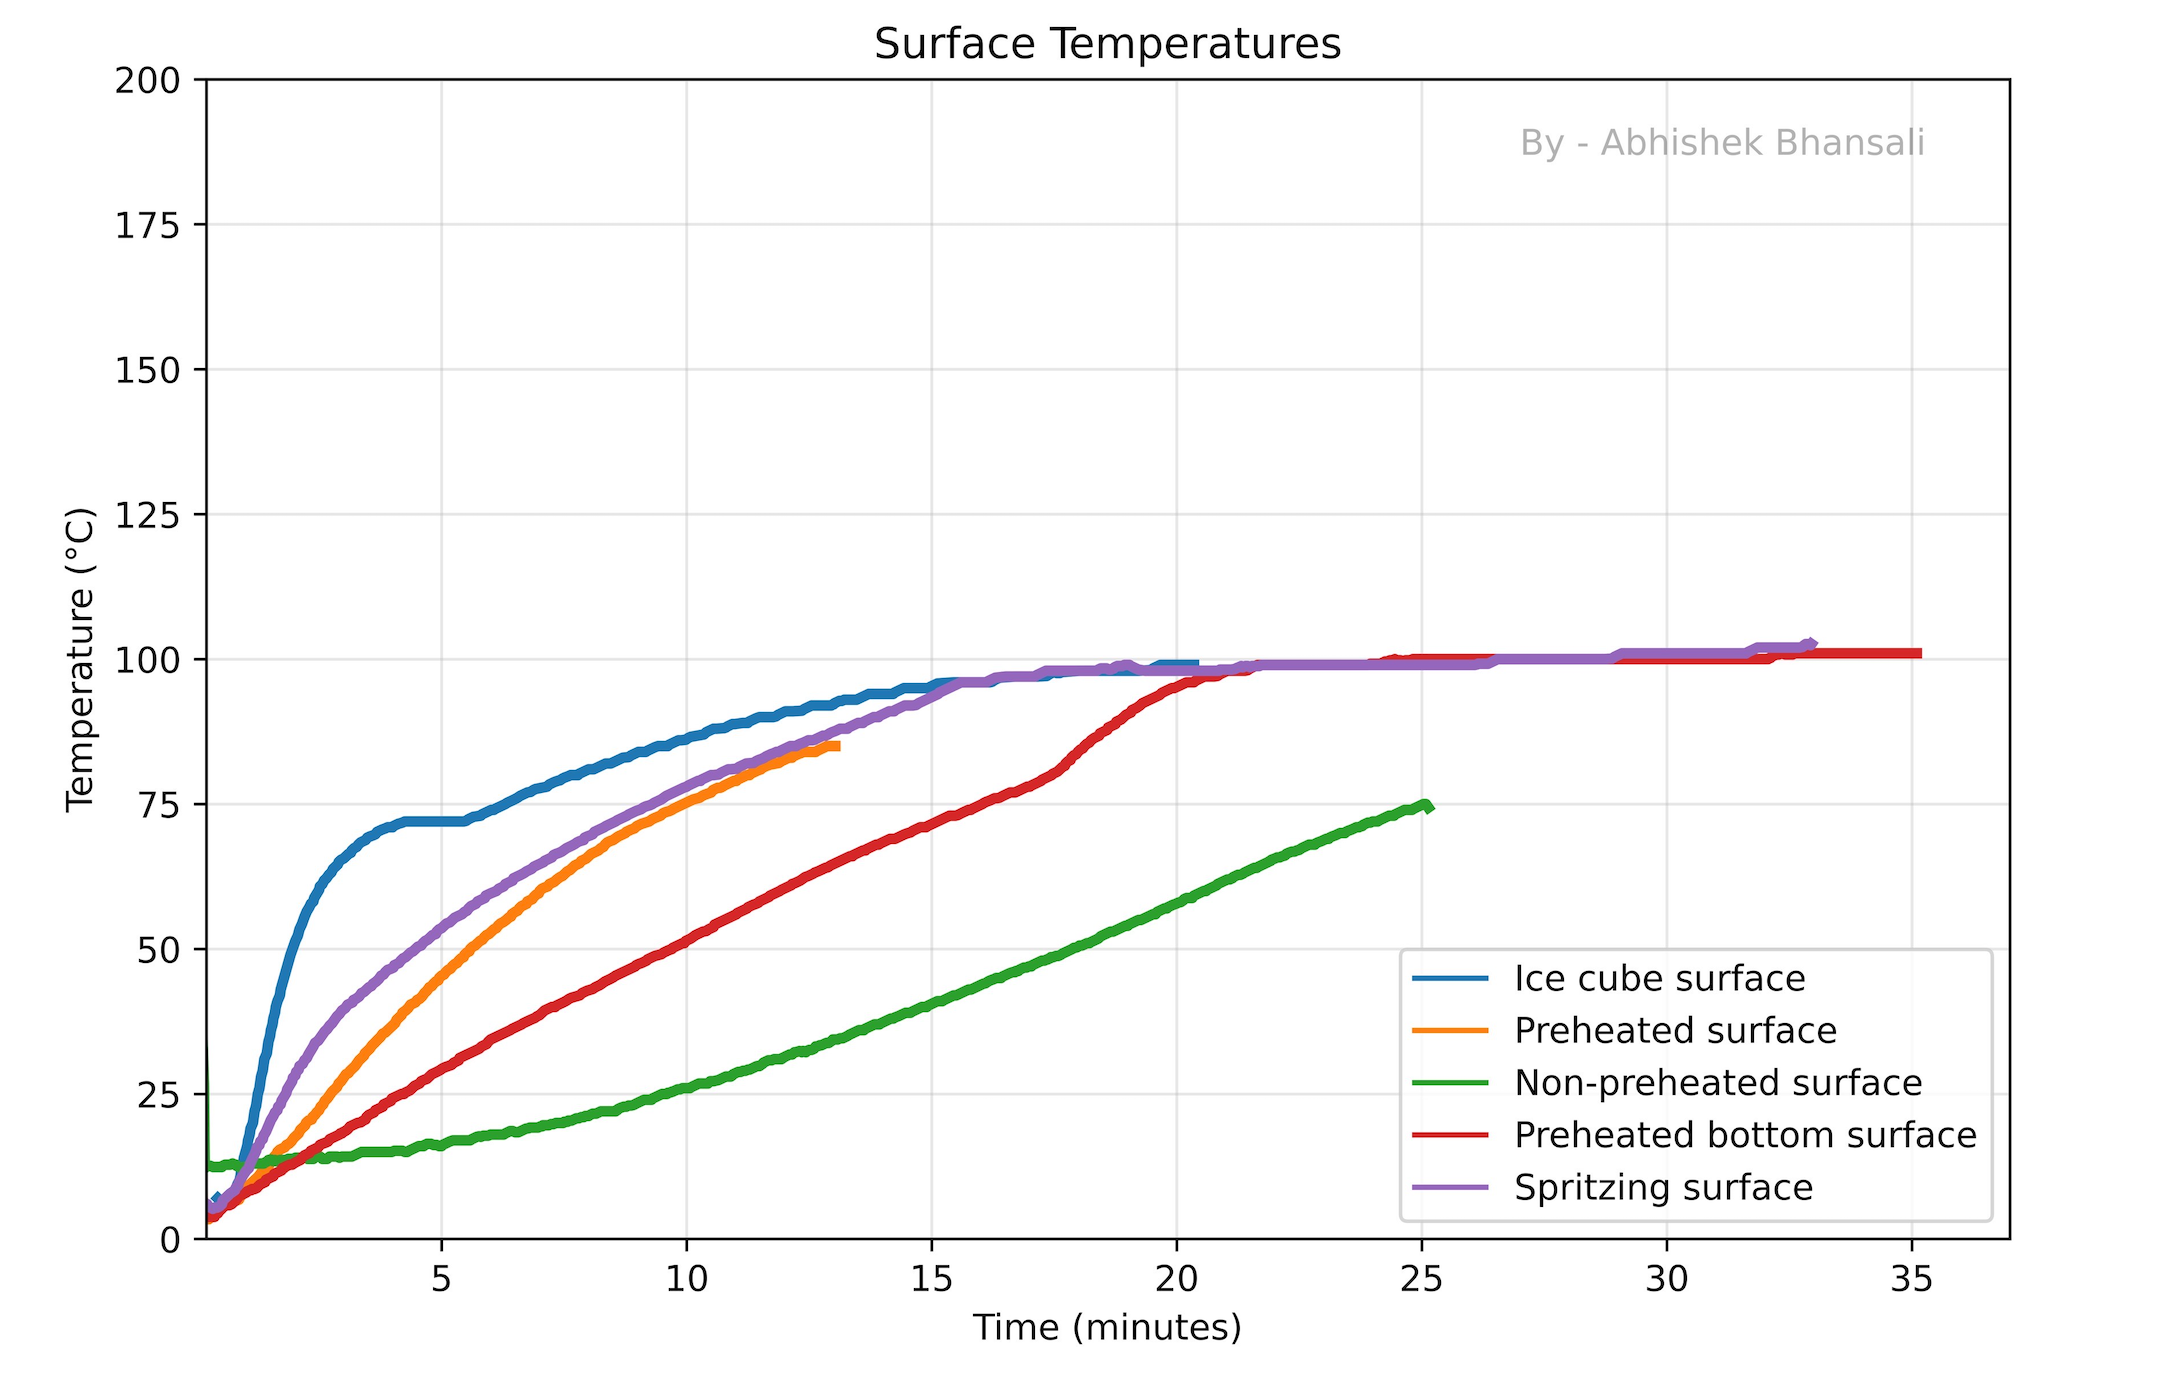
\includegraphics[width=\textwidth]{baking-experiment-temperatures.png}
  \caption{This chart shows how surface temperatures change using
  different steaming methods. In this case I used a dutch oven and an apple as
  dough replacement. All the apples were coming from the fridge. The temperature
  was measured using a barbecue thermometer.
  The more steam the faster the surface temperature increases.}
\end{figure}

It would be a very interesting experiment to bake a bread at different exact
temperatures. How would a bread taste with only evaporated water but
full acidity? What if you were to just completely get rid of the acetic
acid? How would the taste change?

As the temperature increases
the crust thickens. The maillard reaction kicks in further deforming
proteins and starches. The outside of your dough starts to become
browner and crisper. This process begins at around 140°C (284°F)

Once the temperature increases even more to around 170°C (338°F)
the caramelization process begins. The remaining sugars the microbes
did not convert yet start to brown and darken. You can keep baking
for as long as you like to achieve the crust color that you like.
\footnote{This really depends a lot on your personal preference.
Some people prefer a darker crust, others prefer a more pale crust.
It's better to build less crust than too much. You can always just
heat your bread in the oven one more time to continue building a
darker crust.}

The best option to know that your dough is done is to take
the temperature of your dough. You can use a barbecue thermometer
to measure it. Once the core temperature is at around 92°C (197°F)
you can stop the baking process. This is typically not done though
as the crust hasn't been built yet.\footnote{The thermometer is
especially important when using a large loaf pan. It is sometimes
very hard to judge from the outside if the dough is done. I failed
many times and ended up having a semi baked dough.}

Once your dough has finished baking it is ready to eat. Your
dough has turned into a bread. At this
point your bread is sterile as the temperature was too hot for
for the microorganisms to survive.

\section{The role of steam}

Steam is essential when baking as it helps to counter premature
crust building. During the first stage of the bake the dough
increases in size. The water in your dough evaporates and pushes
the whole dough upwards. 

\begin{figure}[!htb]
  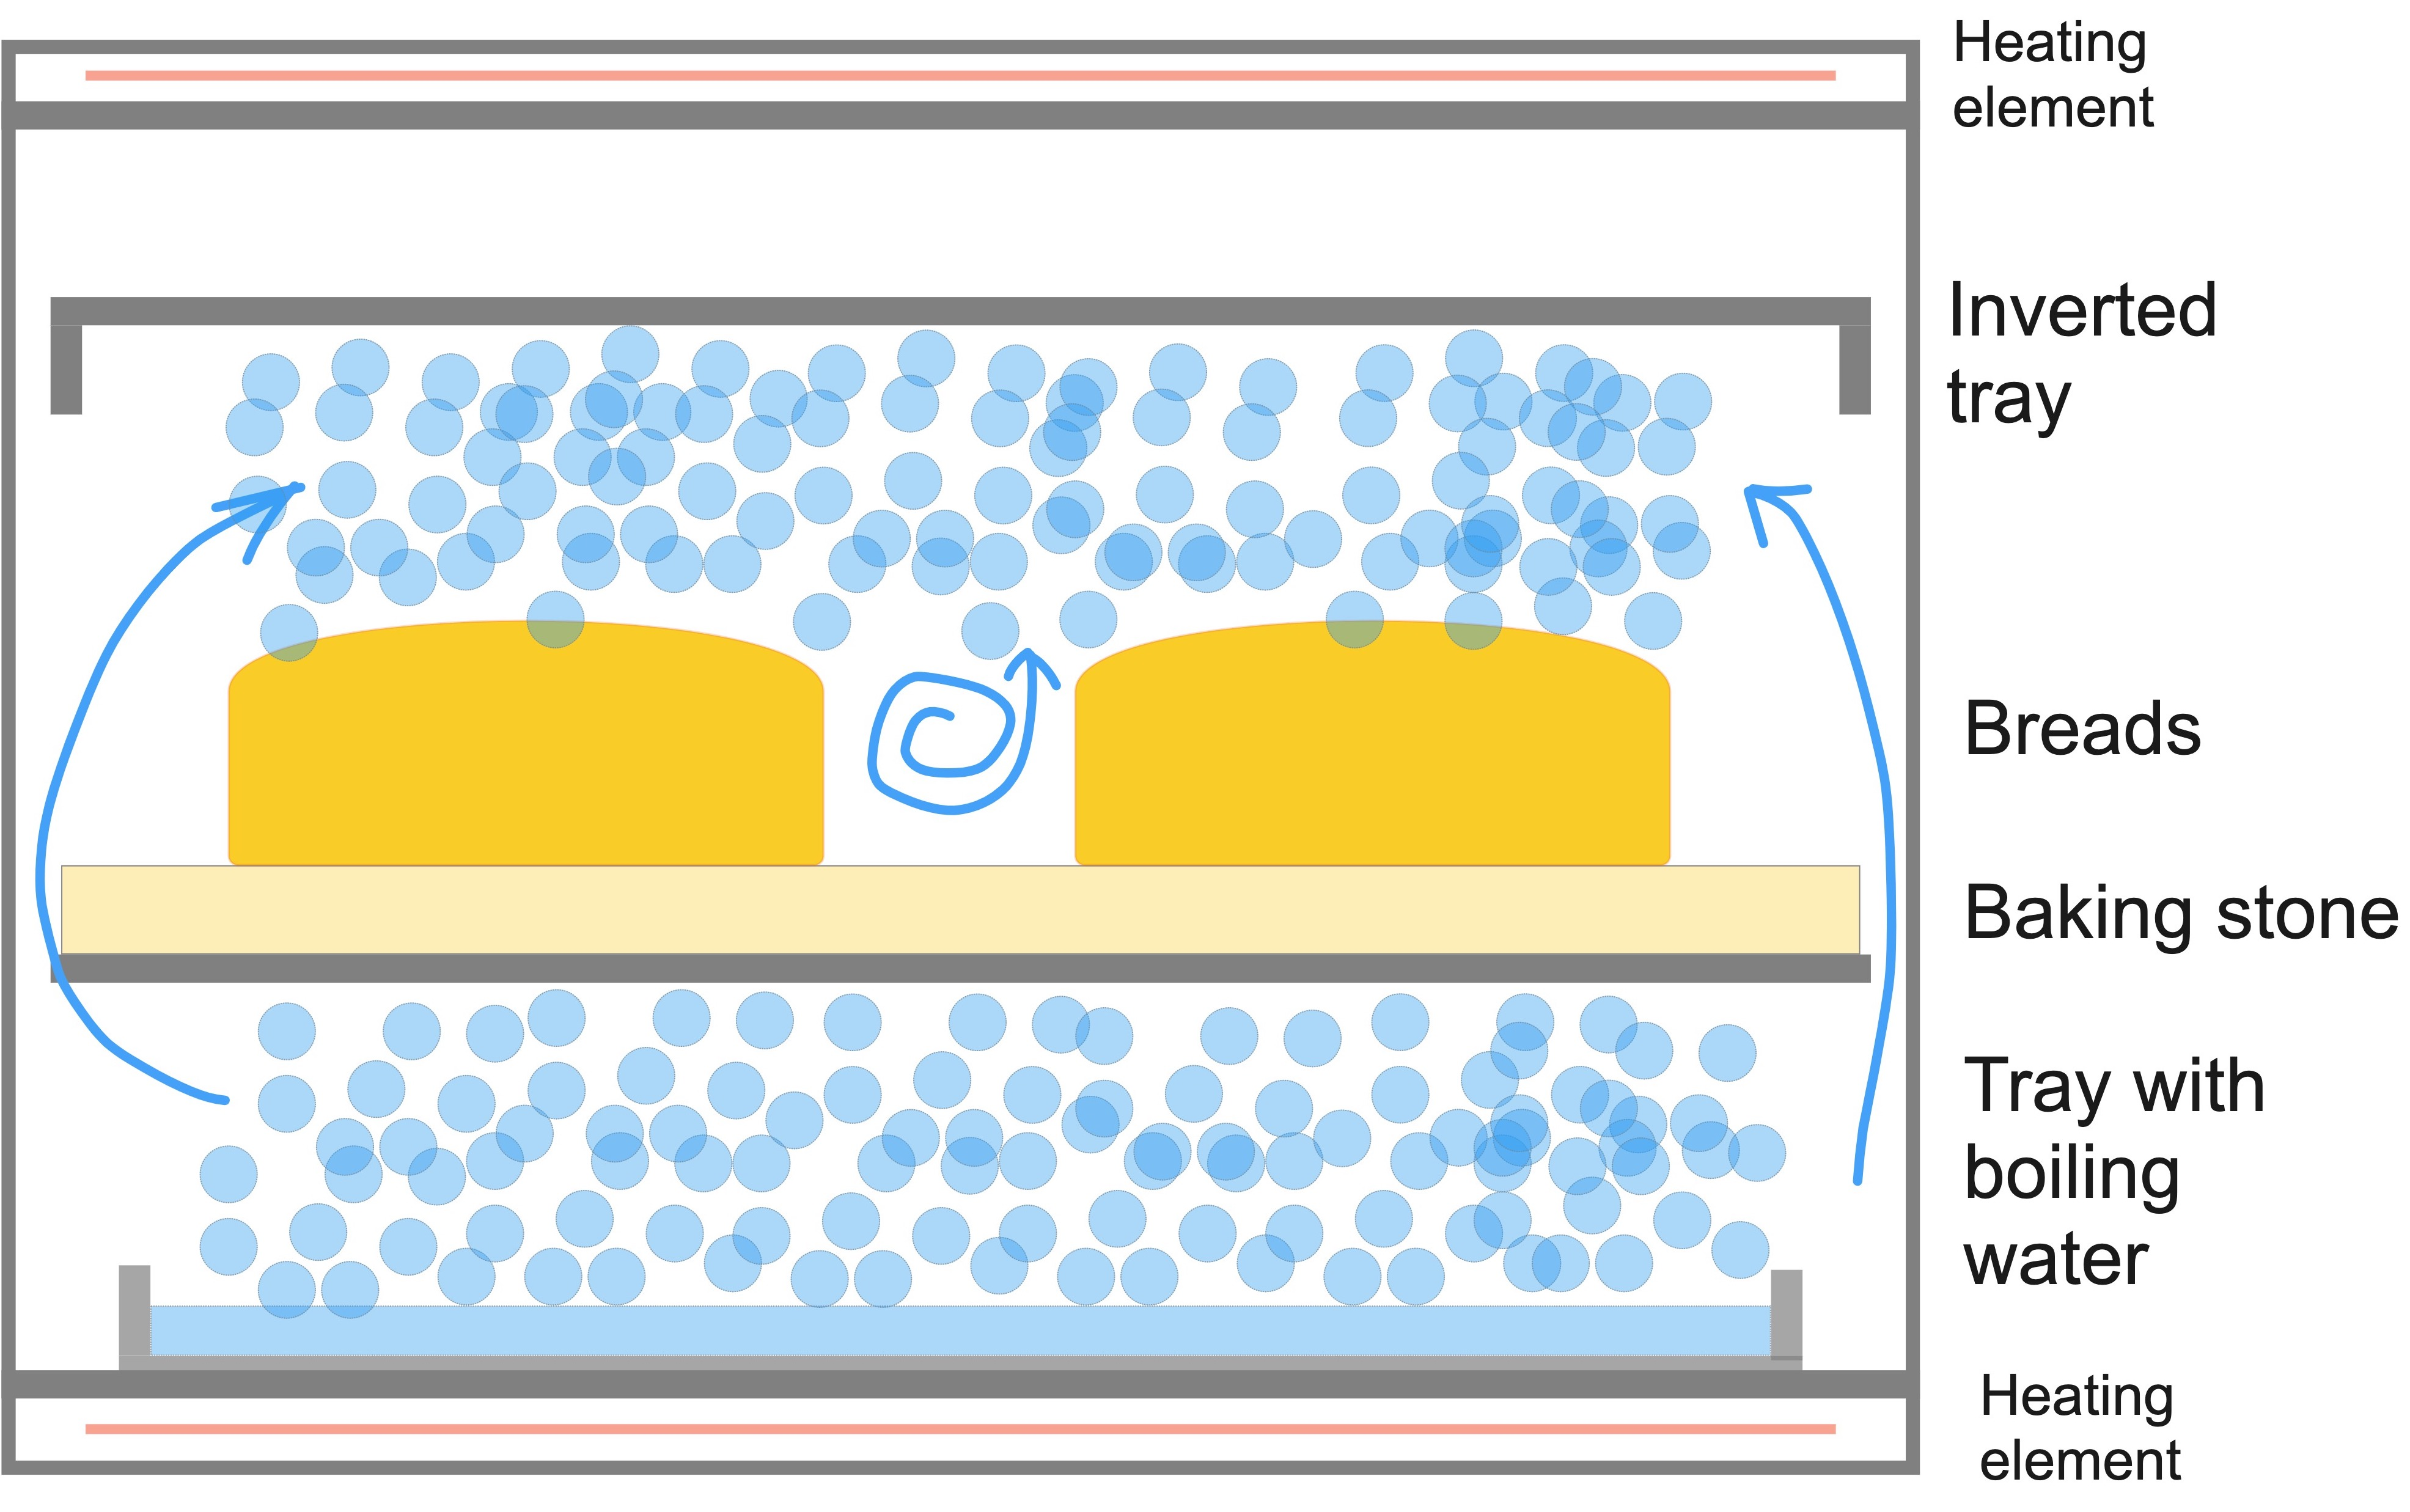
\includegraphics[width=\textwidth]{baking-process-steam.jpg}
  \caption{How steam builds in your oven using the later described
  inverted tray method}
\end{figure}

Normally under high heat a crust would form. Just like
if you were to bake vegetables in your home oven. At some point
they become darker and crisper. This is the same thing that
happens with your dough. You want to delay this process
as long as possible until your dough no longer expands.
Expansion stops when most of the microbes have died and
the evaporating water no longer stays inside the alveoli.
The stronger the gluten network the more gas can be retained
during the baking process. This gluten network at some point
loses its ability to contain gas as the temperature heats
up. The dough stops to increase in size. The steam plays
an important role as it condenses and evaporates on top
of your dough. The surface temperature is rapidly increasing
to around 75°C (160°F). At this temperature the gel starts
to build. This gel is still extensible and allows expansion.
Without the steam the dough would never enter the gel stage,
but instead directly go to the maillard reaction zone. You
want your dough to stay in this gel stage as long as possible
to achieve maximum expansion.\footnote{You can remove your
dough from the oven after 5 minutes to see the gel. You will notice
that it holds the doughs structure. It has a very interesting consistency.}

\begin{figure}[!htb]
  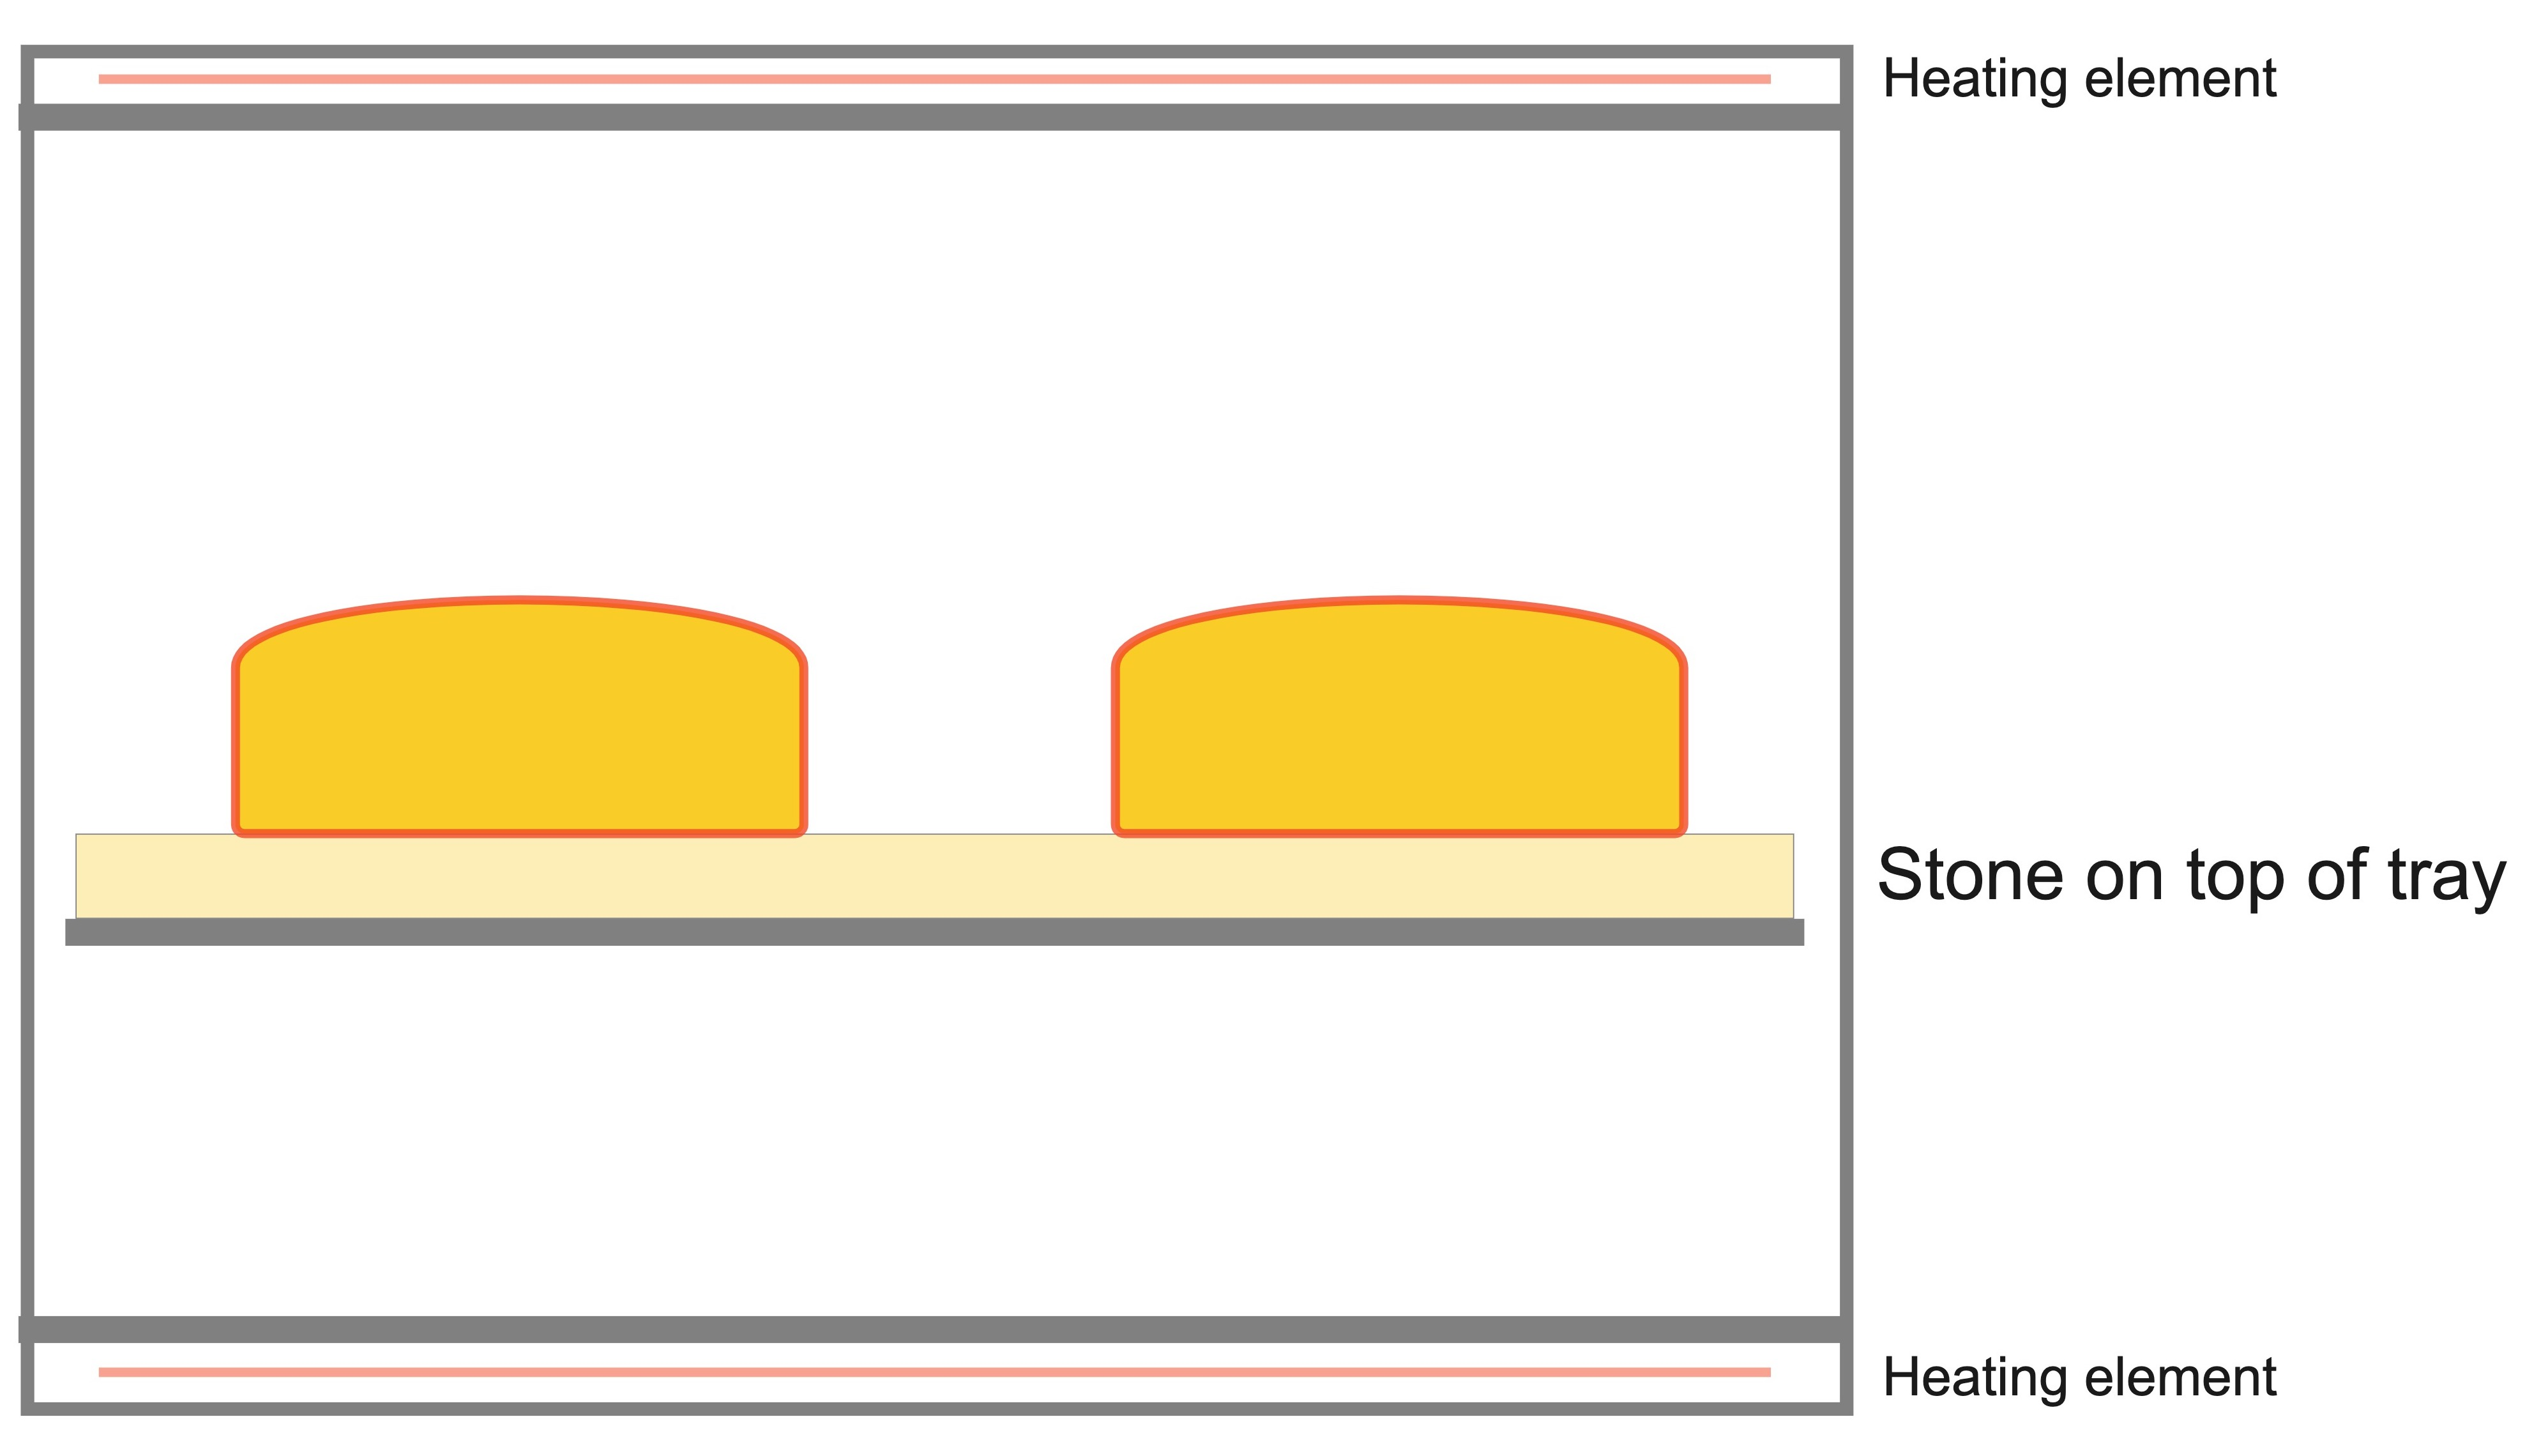
\includegraphics[width=\textwidth]{baking-process-stage-2.jpg}
  \caption{The second stage of the bake is done without steam to build
  a thicker darker crust}
\end{figure}

When not steaming enough you will notice that the scoring
incisions do not properly open up during the bake. They stay
closed as the dough is unable to push through the crust.

Furthermore a common sign is, that you have larger pockets
of air towards the crust of your dough. As the dough increases
vertically expansion is halted by the crust. The pockets
of air converge into larger pockets as pressure increases.
This can also happen when you are baking at a too hot temperature.

The more you steam the softer your dough's crust is. You will never
enter the maillard and caramelization stage. This
is the reason why the source of steam is removed
for the second stage of the bake. No more expansion can
happen and you can focus on building a crust. If you
would like a soft crust you can steam your dough all the
way.

\begin{figure}[!htb]
  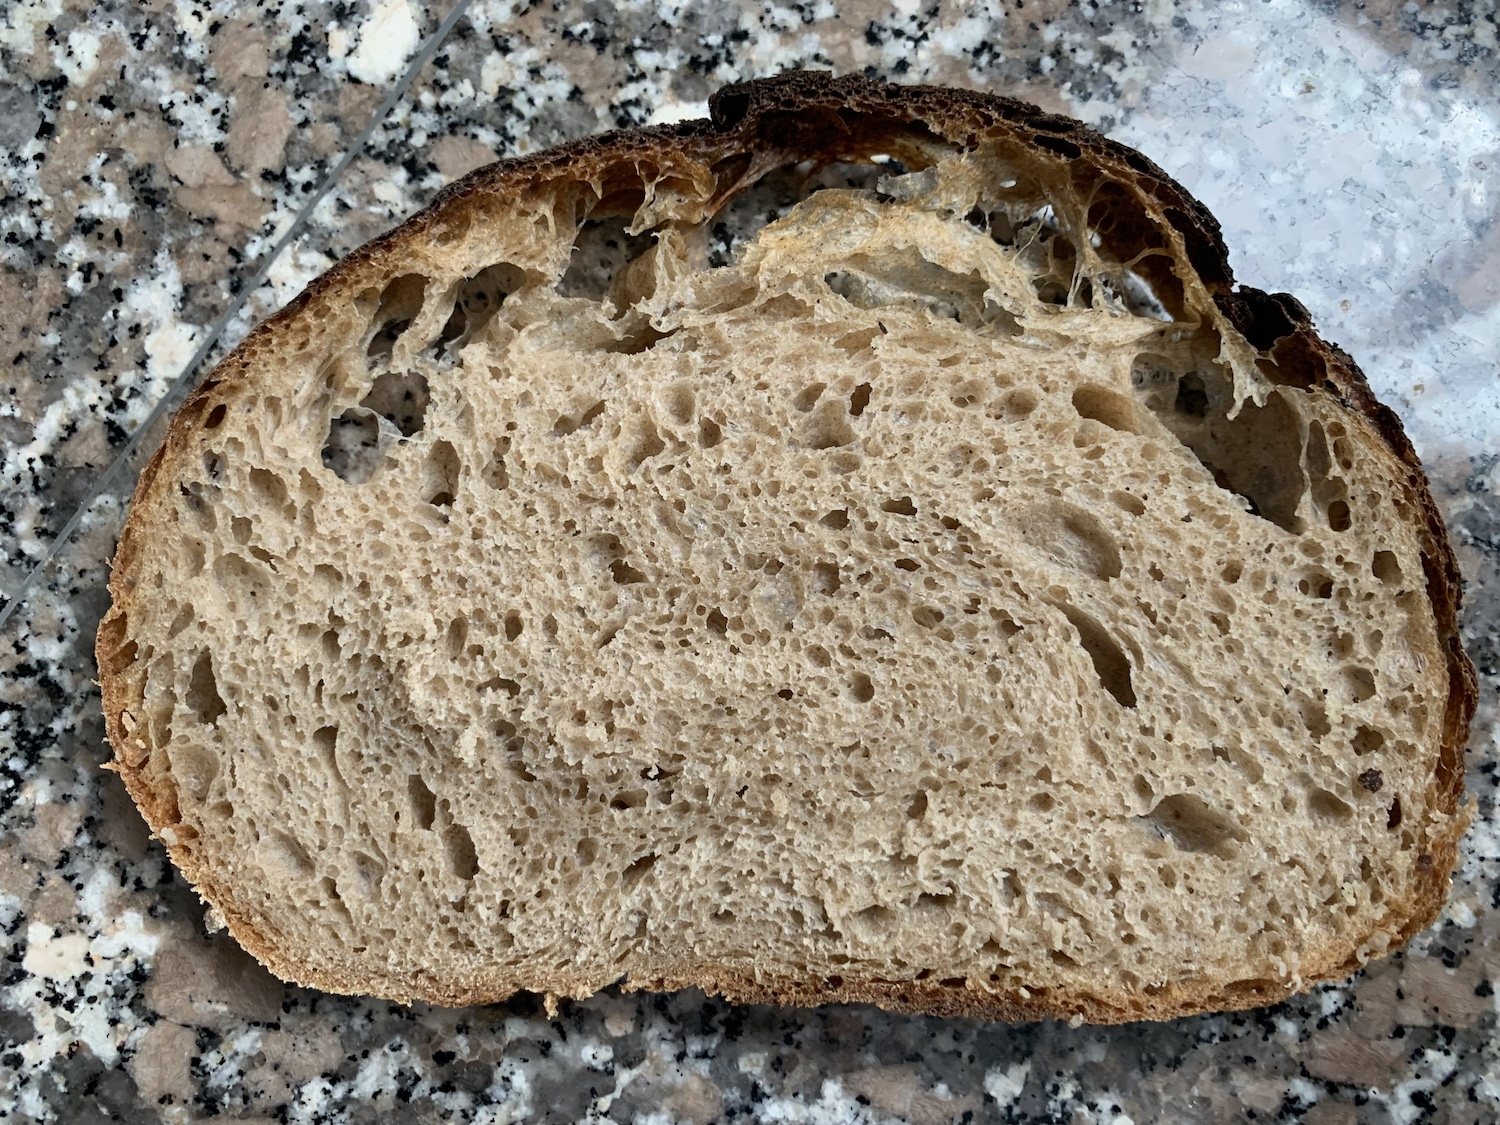
\includegraphics[width=\textwidth]{baking-too-hot.jpeg}
  \caption{A submission by Karomizu showing a bread that has been baked
  at a too hot temperature or with too little steam. Note the large
  pockets of air towards the crust. They are a typical indicator.}
\end{figure}

\section{Dutch ovens}

Dutch ovens are an ideal way to bake with a lot of
steam. They are not fully sealed. Regardless though
as water evaporates from your dough it will create a steamy
environment allowing your dough to rise. It really
makes baking in a home oven very easy.

When using a dutch oven make sure to preheat it properly,
this way your dough will not stick to it. You can also
use additional semolina flour or parchment paper. Another
good trick is to spritz your dough with a bit of water.
To create more steam you could also place a small ice cube
next to your main dough.

I have been using a dutch oven myself for a long time. They
have issues though. They are relatively heavy. It is dangerous
to operate hot cast iron ovens. Especially when working with steam
you have to be very careful.  Furthermore
they are expensive to buy. Then your dutch oven is made out
of cast iron you have to season it from time to time. This takes
time.

The biggest disadvantage though is
capacity. You can only bake a single bread at the
same time. In many cases it makes sense to bake multiple
loaves in one go. It makes the whole process more
efficient as you have to knead less per loaf. The time it
takes to make one bread significantly reduces. Furthermore
you don't require as much energy. You don't have
to preheat your oven twice for each individual loaf.


\section{Inverted tray method}

The inverted tray method simulates a dutch oven.
By placing another tray on top of your dough the steam
created from the dough and water source stays
around your dough.

\begin{figure}[!htb]
  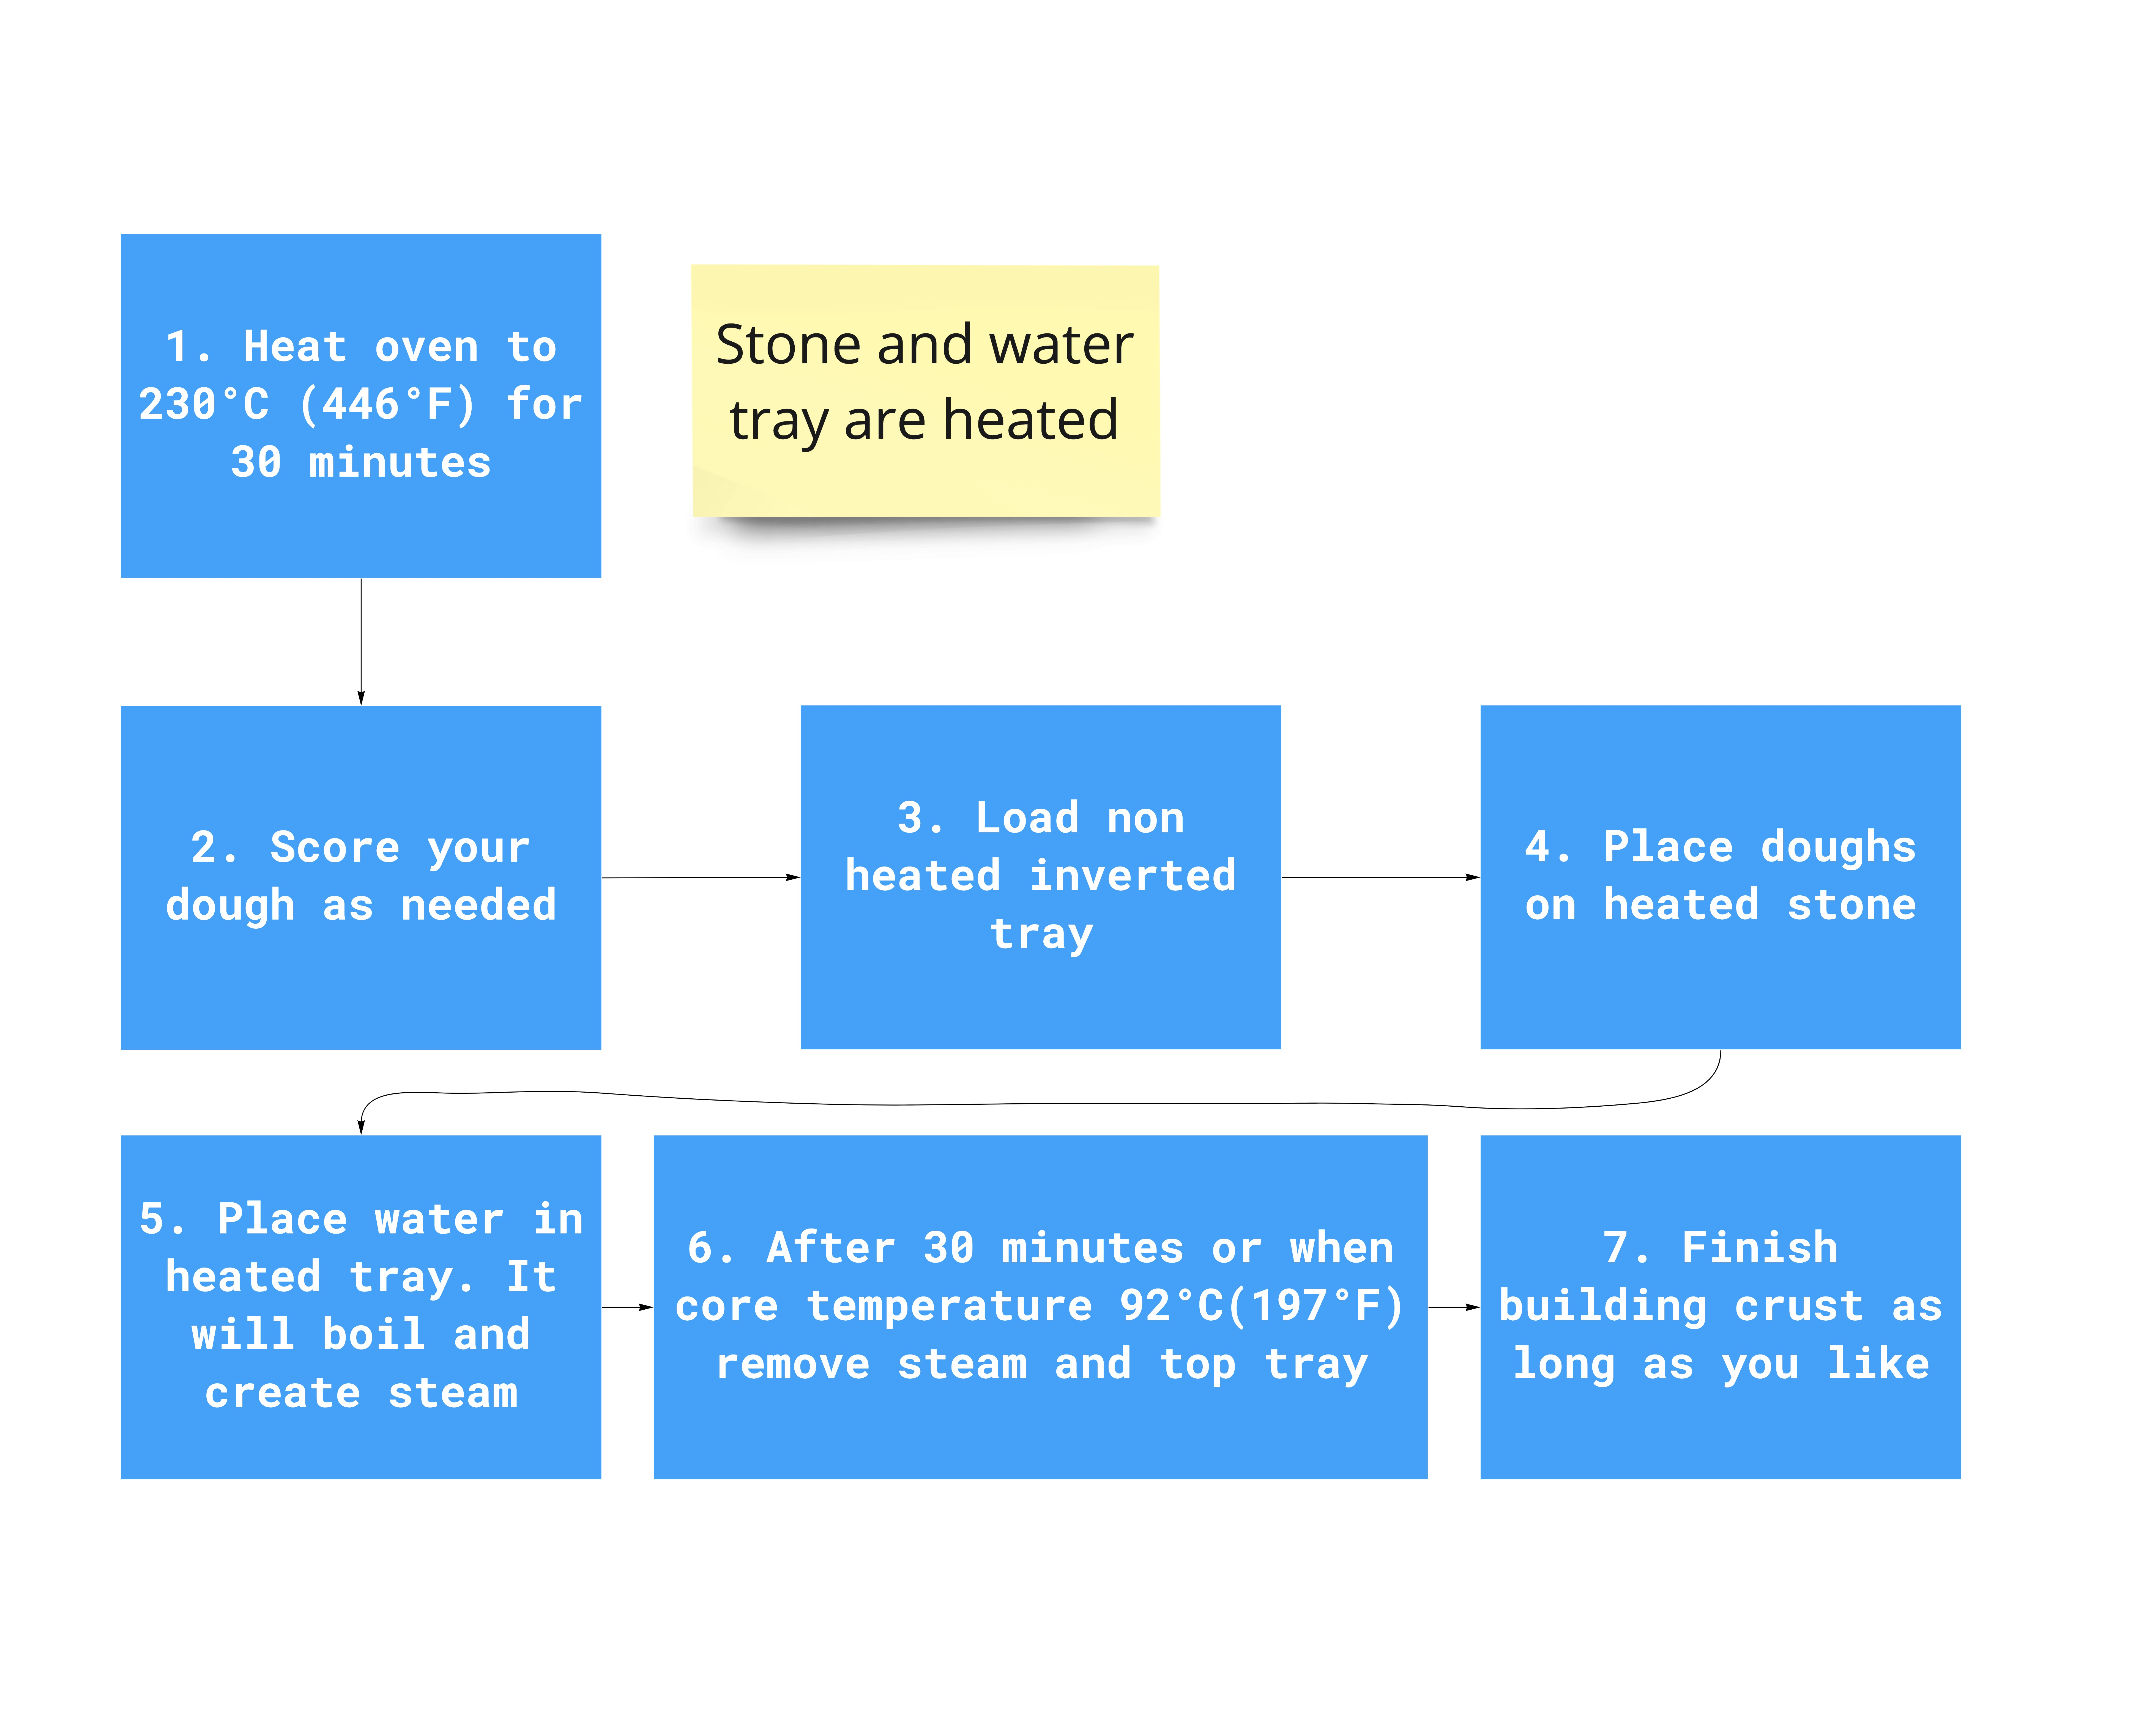
\includegraphics[width=\textwidth]{baking-process-overview.jpg}
  \caption{The full inverted tray method process}
\end{figure}


The biggest advantage of this method compared to the
dutch oven is scalability. You can bake multiple loaves
at the same time. In my case that is around 2 freestanding
loaves and 4 loaves in a loaf pan.

For the inverted tray you will need the following tools:
\begin{itemize}
\item 2 trays
\item 1 heat resistant bowl
\item Boiling water
\item Oven gloves
\item Optional parchment paper
\end{itemize}

\begin{figure}[!htb]
  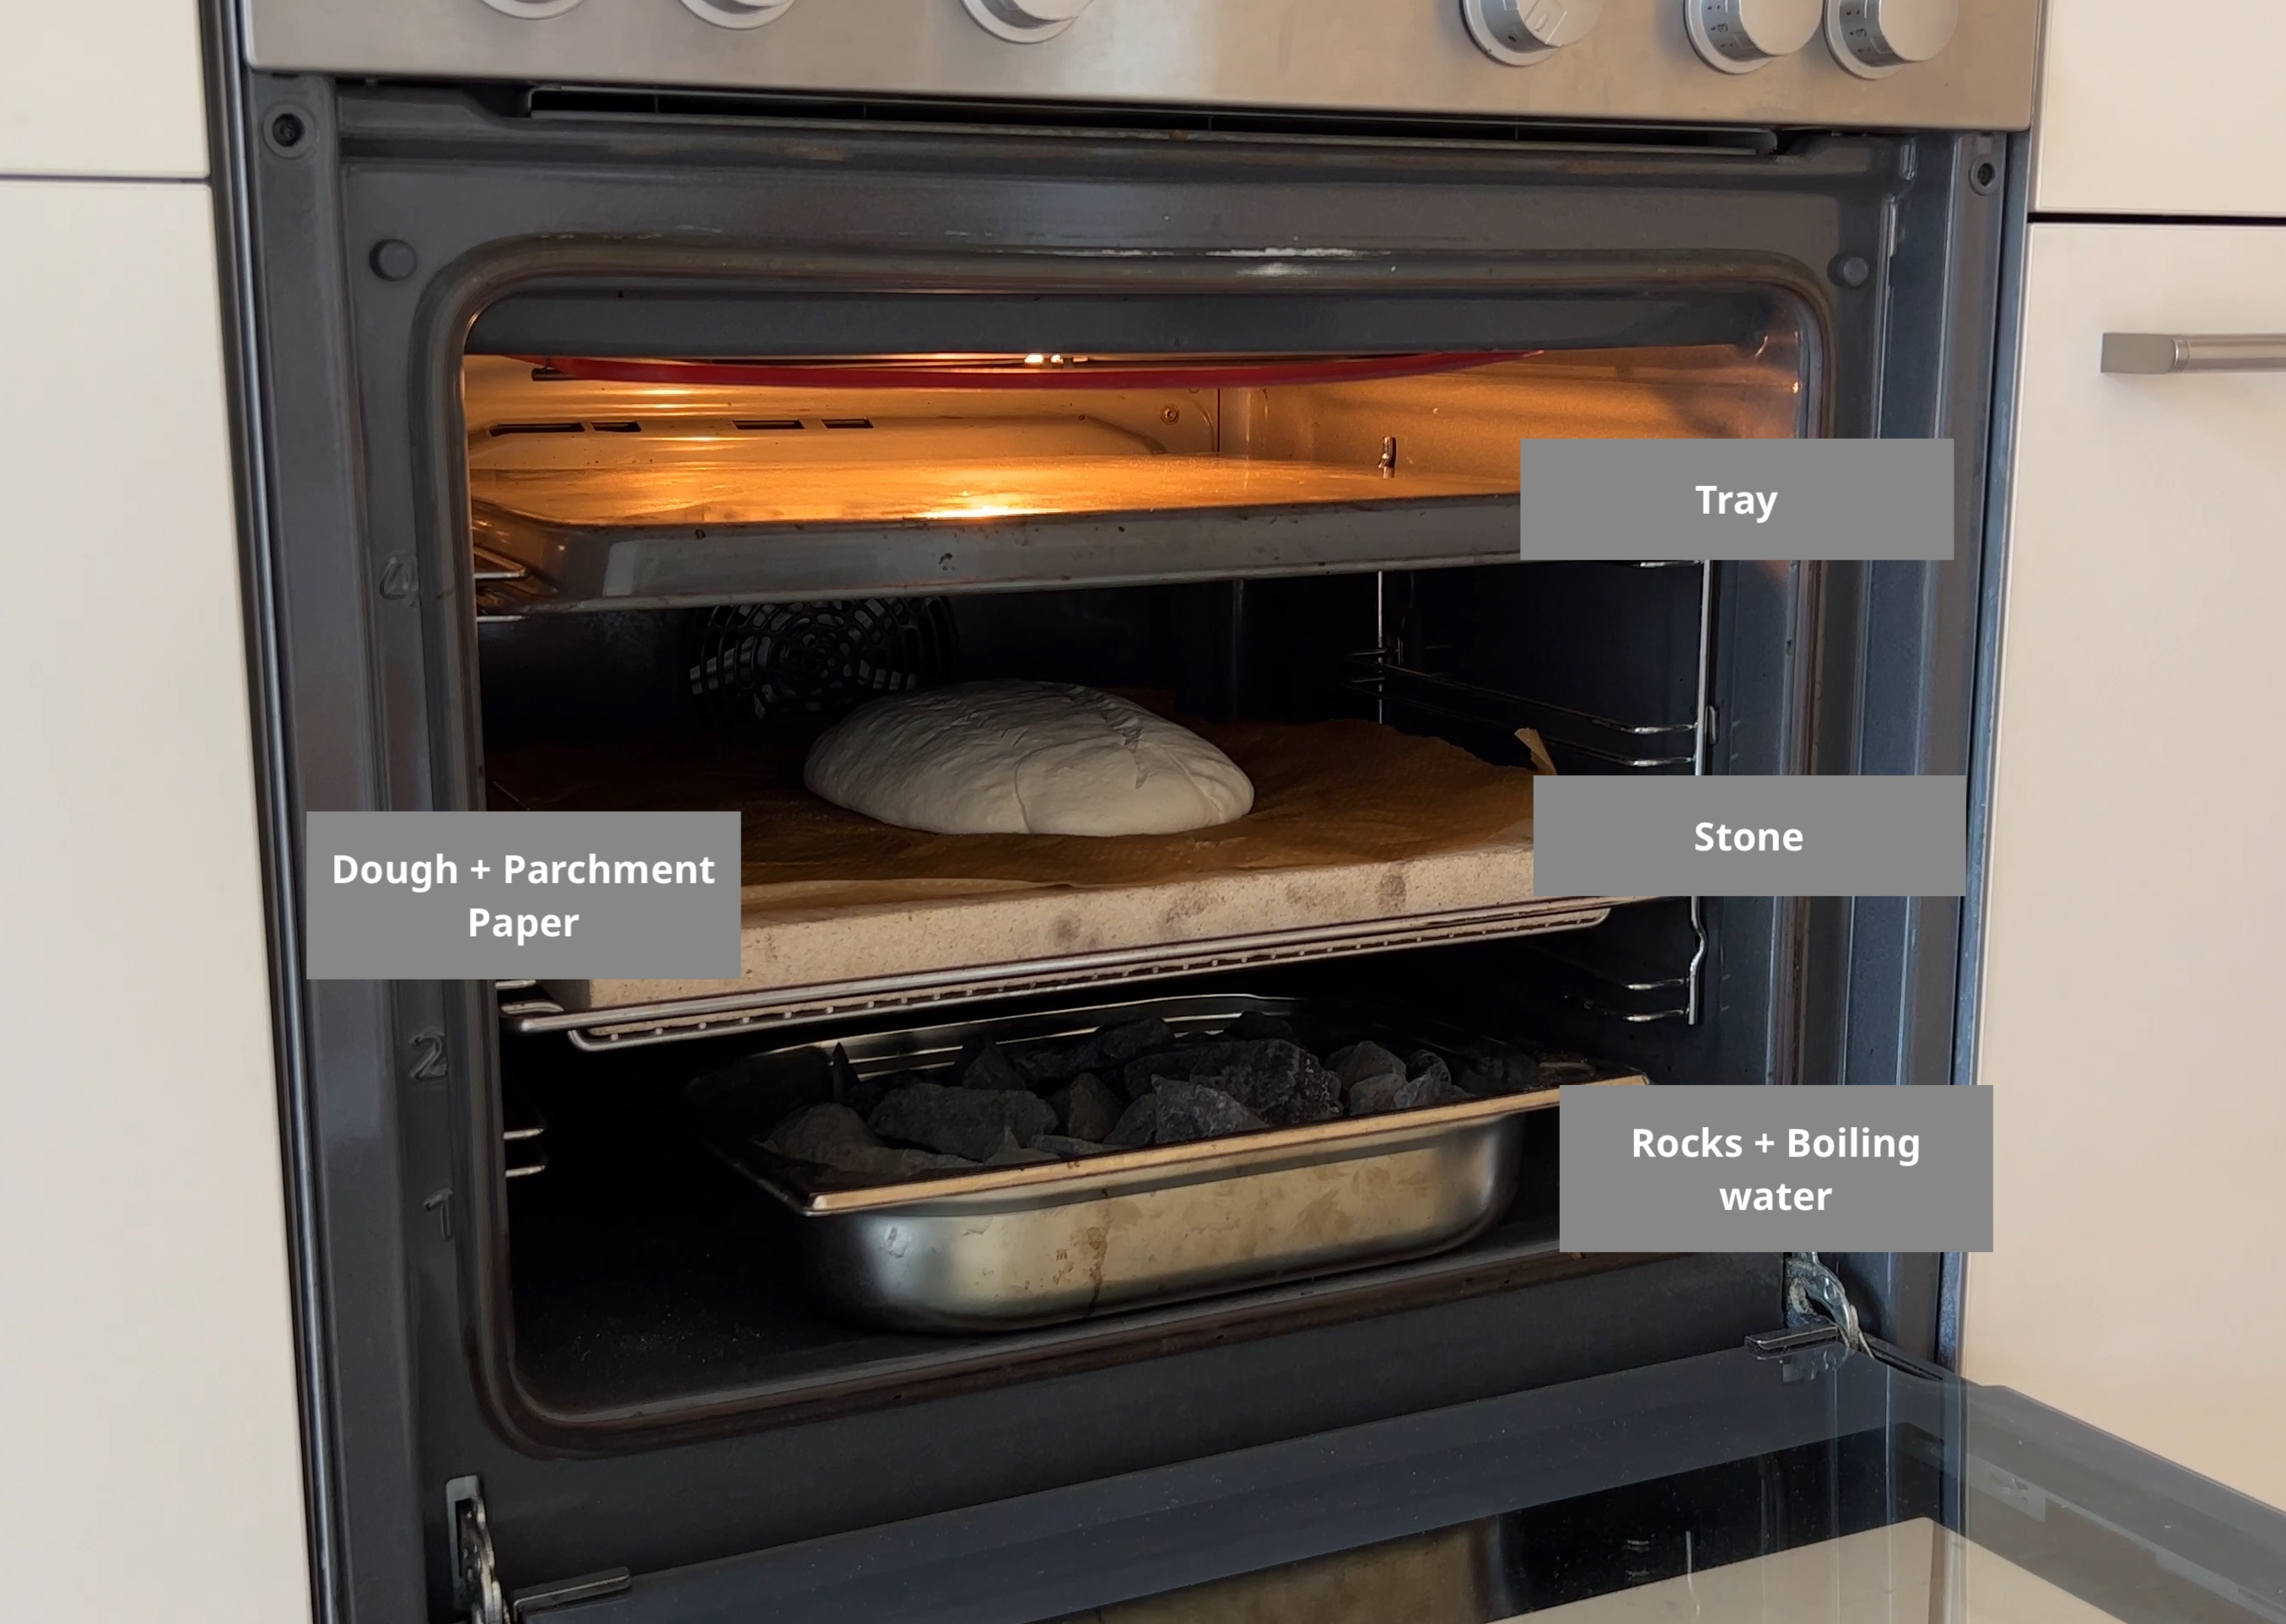
\includegraphics[width=\textwidth]{baking-example.jpg}
  \caption{My home oven setup}
\end{figure}

These are the steps to follow with the inverted tray method
\begin{enumerate}
\item Preheat the the oven to around 230°C (446°F)
Preheat one of the trays
\item Bring water to boil
\item Place your doughs on a piece of parchment paper. You
can also place each on a tiny piece of parchment paper
this makes loading the dough easier. If you don't
have it or don't want to use it, you can opt for 
semolina flour. It helps to make the tray non stick
\item Take out your hot tray and place it
on a cooling rack, or on something else that
is heat resistant
\item Score your doughs
\item Place your doughs on the hot tray
\item Place the cold tray in your oven in an inverted position
\item Move your hot tray including the loaves back
to the oven
\item Place the boiling water in the heat resistant
water bowl. I have added rocks to it, it helps
to improve the steam even further. This is optional
\item Close the oven
\item After 30 minutes remove the top tray. Also remove the bowl with water
\item Finish baking your bread until you have reached your desired
crust color. In my case this is another 15-25 minutes typically.
\end{enumerate}

\section{Conclusions}

\begin{table}[]
  \centering
  \resizebox{\textwidth}{!}{%
  \begin{tabular}{|l|l|l|l|}
  \hline
  \textbf{Oven type}                                                         & \textbf{Plain (no tools)} & \textbf{Inverted tray} & \textbf{Dutch oven} \\ \hline
  Gas                                                                        & No                        & No                     & Yes                 \\ \hline
  \begin{tabular}[c]{@{}l@{}}Convection\\ (Fan always on)\end{tabular}       & No                        & No                     & Yes                 \\ \hline
  \begin{tabular}[c]{@{}l@{}}Convection\\ (Fan can be disabled)\end{tabular} & No                        & Yes                    & Yes                 \\ \hline
  Steam                                                                      & Yes                       & Yes                    & Yes                 \\ \hline
  \end{tabular}%
  }
  \caption{An overview of ovens and their different baking methods}
\end{table}

Depending on your home oven a different method
of steaming should be used. Generally most ovens
are made to vent out most of the steam during the
bake. They are typically not fully closed. During
baking you want to dry out whatever you are baking.
This is ideal if you are baking vegetables and
want them to dry out. For baking though this is
highly problematic. As described earlier, you
want there to be as much steam as possible.

If you are using a gas based oven the only option
is to utilize a dutch oven. The same is true when you
are using a convection oven with a fan that
can not be disabled. When using a convection
oven with a fan that can be turned off, you can
opt to use the cost efficient inverted tray
method.

If you are in the luxurious
position to own a steam oven, things are easier.
Just activate the steam function and you are
good to go. Placing an additional tray on top of your
dough during the bake helps to bake with indirect
heat. You remain in the gel zone longer and
will experience more oven spring.

\chapter{Storing bread}
\section{Fridge}
\section{Room temperature}
\section{Frozen}

\chapter{Troubleshooting}

The crumb structure of your bread provides insights on how well
your fermentation process has gone. You can also spot common flaws
of improper technique. This chapter will provide you with information
that you can use to debug your baking process.

\subsection{Perfect fermentation}

\begin{figure}
  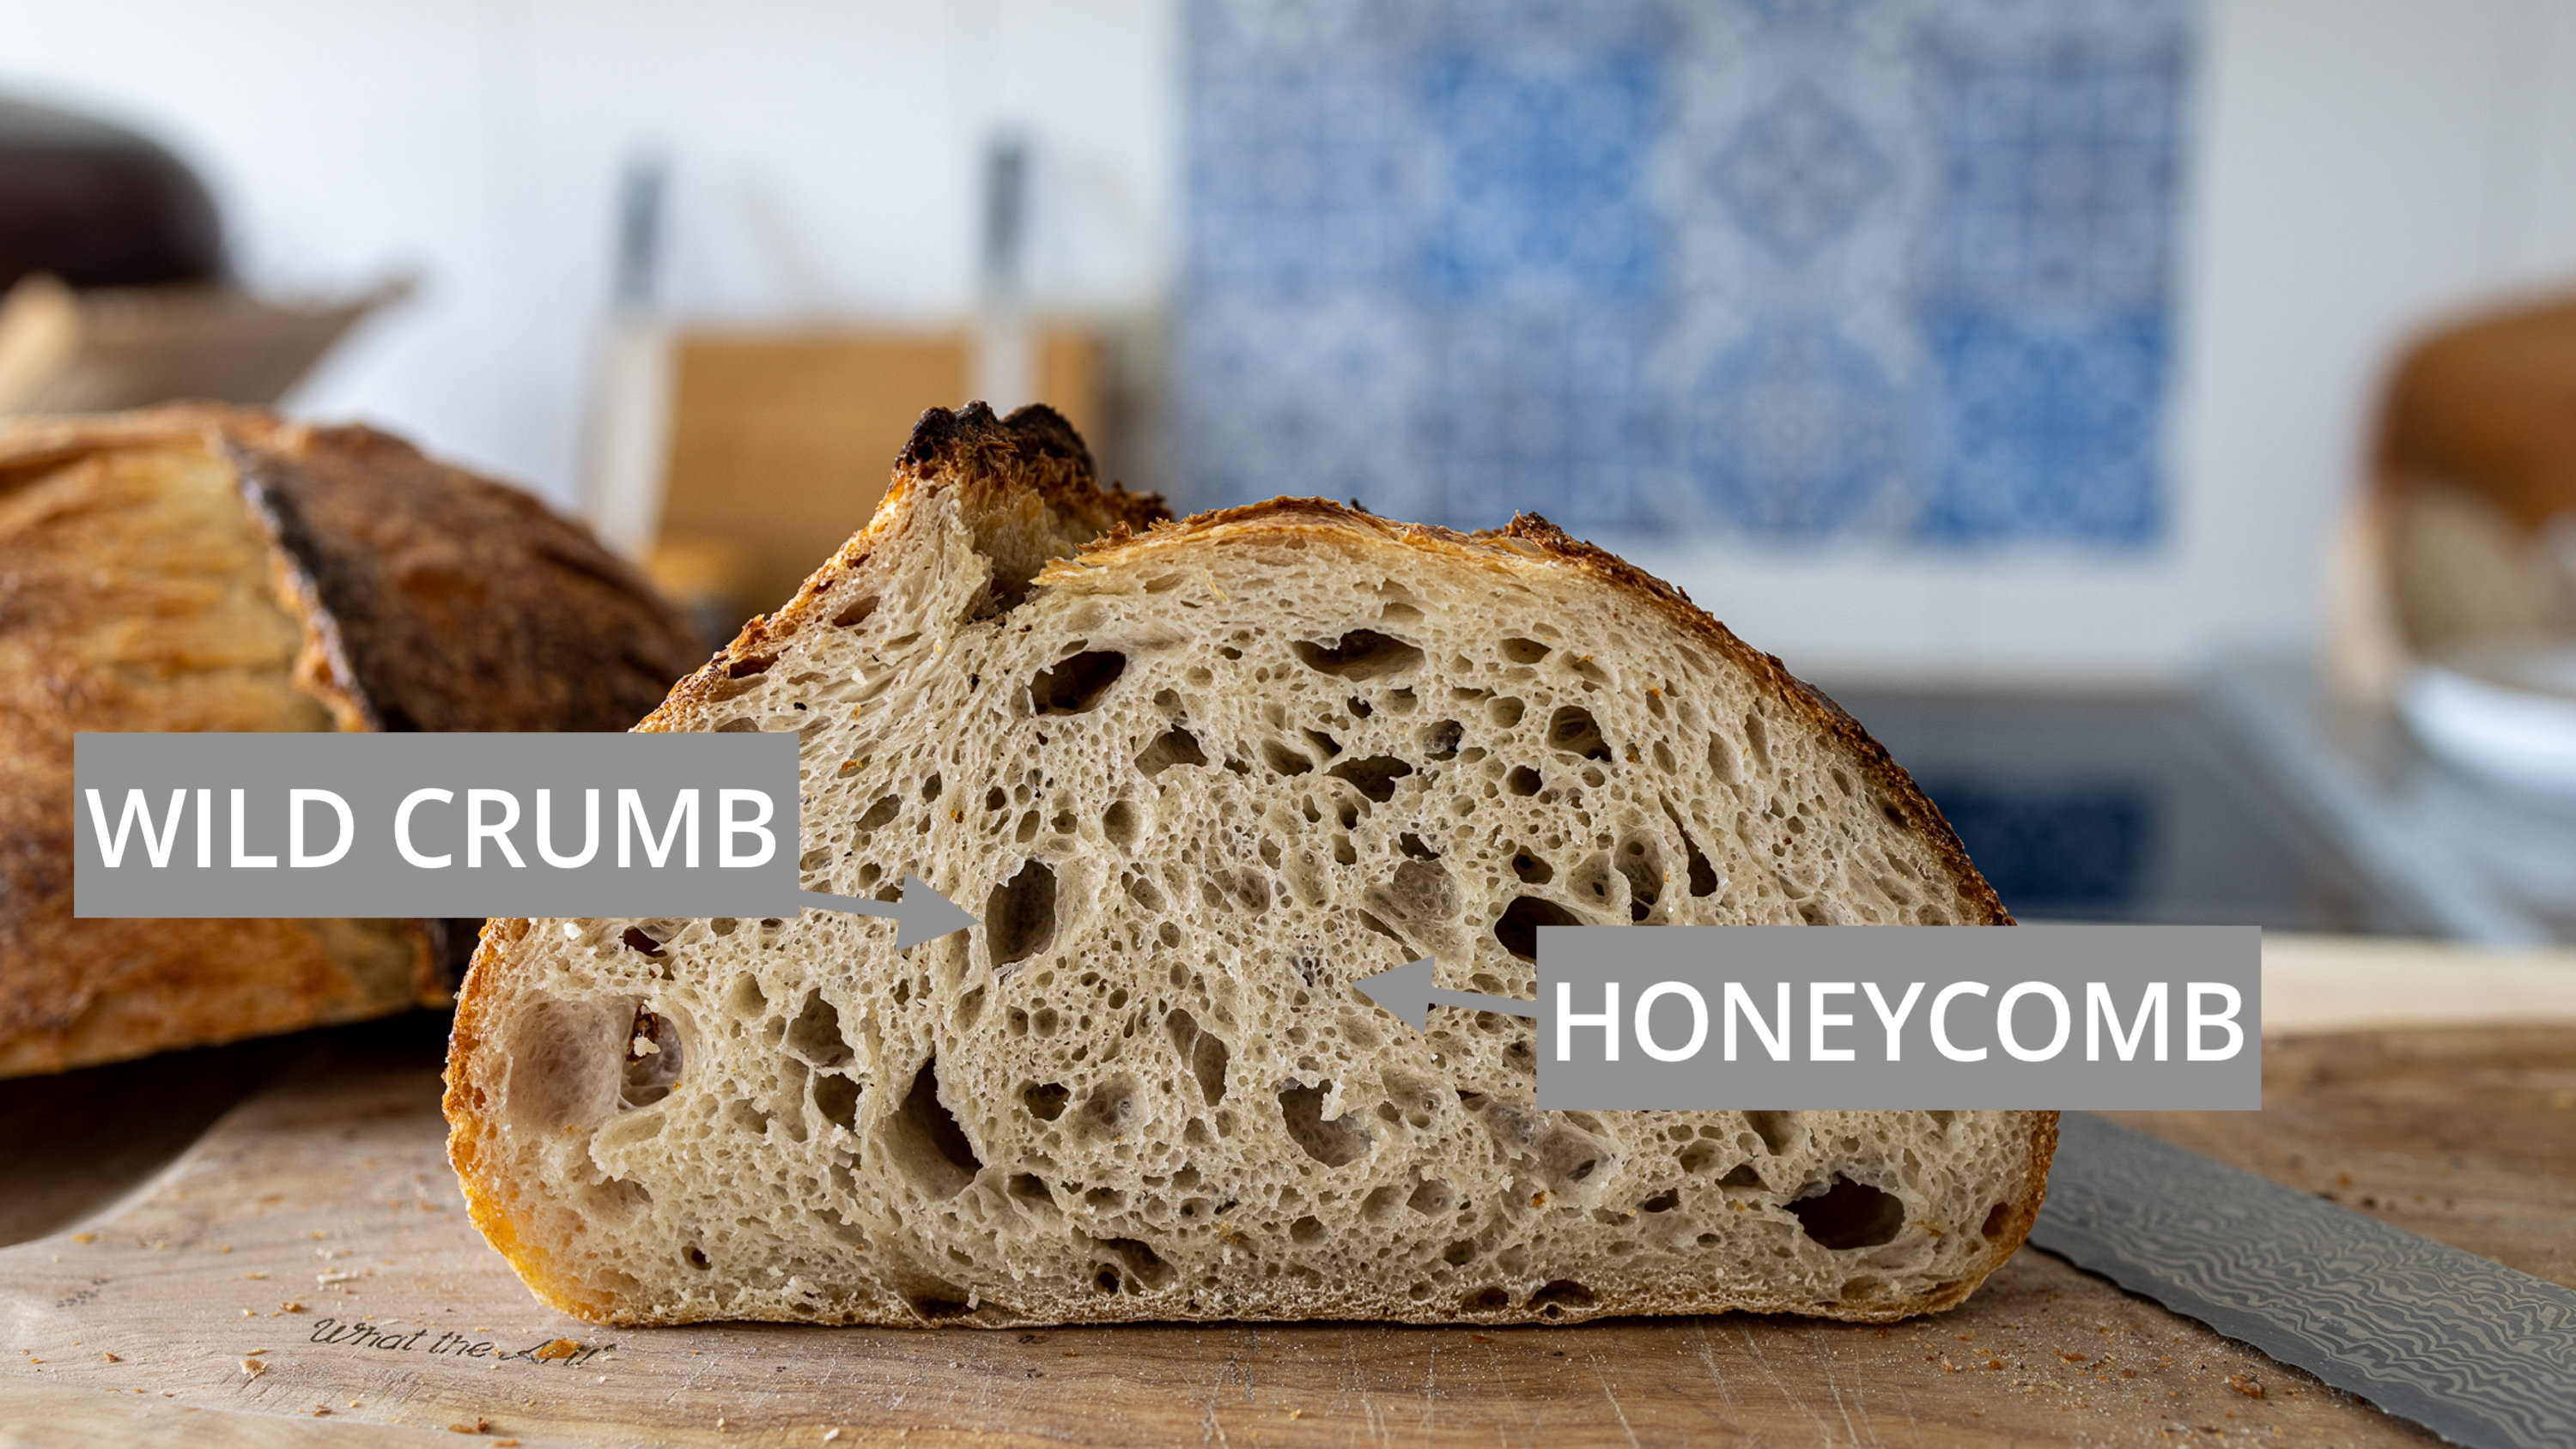
\includegraphics[width=\textwidth]{open-crumb}
  \caption{The bread has a somewhat open crumb with areas
  featuring a honeycomb structure.}
  \label{fig:open-crumb}
\end{figure}

Of course the perfect fermentation is debatable and highly subjective. To
me the perfect sourdough bread features a crisp crust paired with a fluffy
somewhat open crumb. This is the perfect balance of different consistencies
when you take a bite.

Some people are chasers of a very open crumb, meaning you have large pockets
of air (alveoli). It's subjective whether that's the style of bread that you like,
however to achieve it you need to ferment your bread dough perfectly on point.
It takes a lot of skill both in terms of mastering fermentation and technique
to achieve a crumb structure like that.

Me personally I like a bread like that, just with a slightly less wild crumb.
The style of crumb I like is called the {\it honeycomb crumb}. It's not too open, but
just enough open to make the bread very fluffy. To achieve the previously mentioned open crumb you
have to touch your dough as little as possible. The more you interact with your
dough the more you are degassing your dough. Excess touching of the dough
results in the dough's alveoli merging together. The crumb will not be as open.
That's why achieving such a crumb works best if you only ferment
one dough at the same time. Normally if you have to preshape your dough,
you will automatically degas your dough a little bit during the rounding process.
If you skip this step and directly shape your dough you will achieve a more open crumb.
A good rule of thumb is to not touch your dough for at least 1-2 hours before shaping,
to achieve an as open crumb as possible.

\begin{figure}
  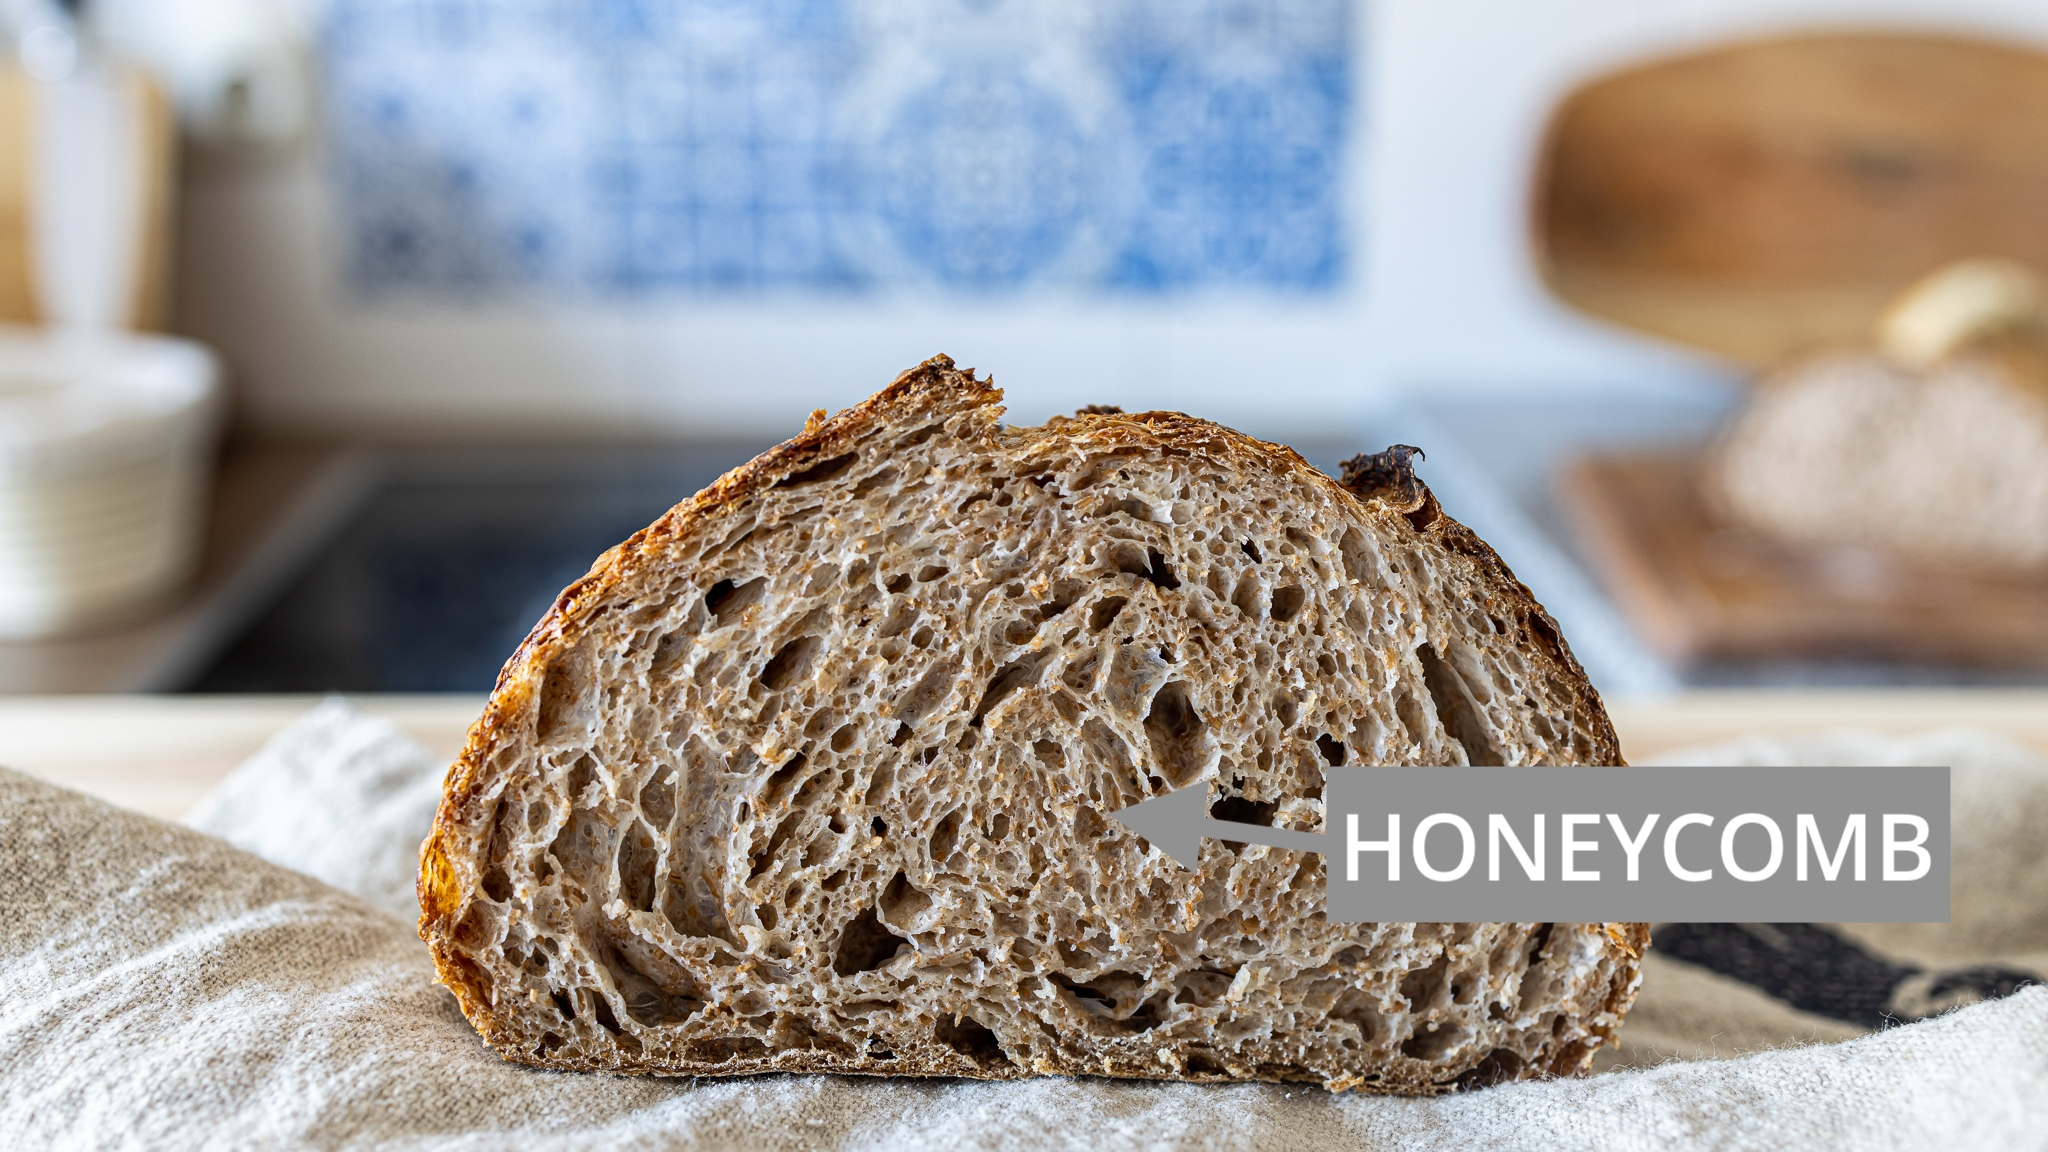
\includegraphics[width=\textwidth]{honeycomb}
  \caption{A whole wheat sourdough with an almost exclusive honeycomb crumb structure.}
  \label{fig:honeycomb}
\end{figure}


Now this is problematic when you want to
make multiple breads at the same time. Preshaping is essential as you are required
to divide your large bulk dough into smaller chunks. Without the preshaping
process you would end up with many non-uniform bread doughs. This technique is
also used when making ciabattas. They are typically not shaped. You only cut the
bulk dough into smaller pieces, trying to work the dough as little as possible.
With preshaping you will converge your dough's alveoli into more of a honeycomb structure,
as large pockets of air will slightly converge. Similarly to the open crumb structure
you also have to nail the fermentation process perfectly to achieve this crumb.
A too long fermentation will result in gas leaking out of your dough while baking.
The honeycomb's won't be able to retain the gas. If you ferment for too short,
there is not enough gas to inflate the structures. To me this is the perfect
style of crumb. As someone who appreciates jam, no jam will fall through a slice
of this bread compared to an open crumb.

\subsection{Overfermented}

\begin{figure}
  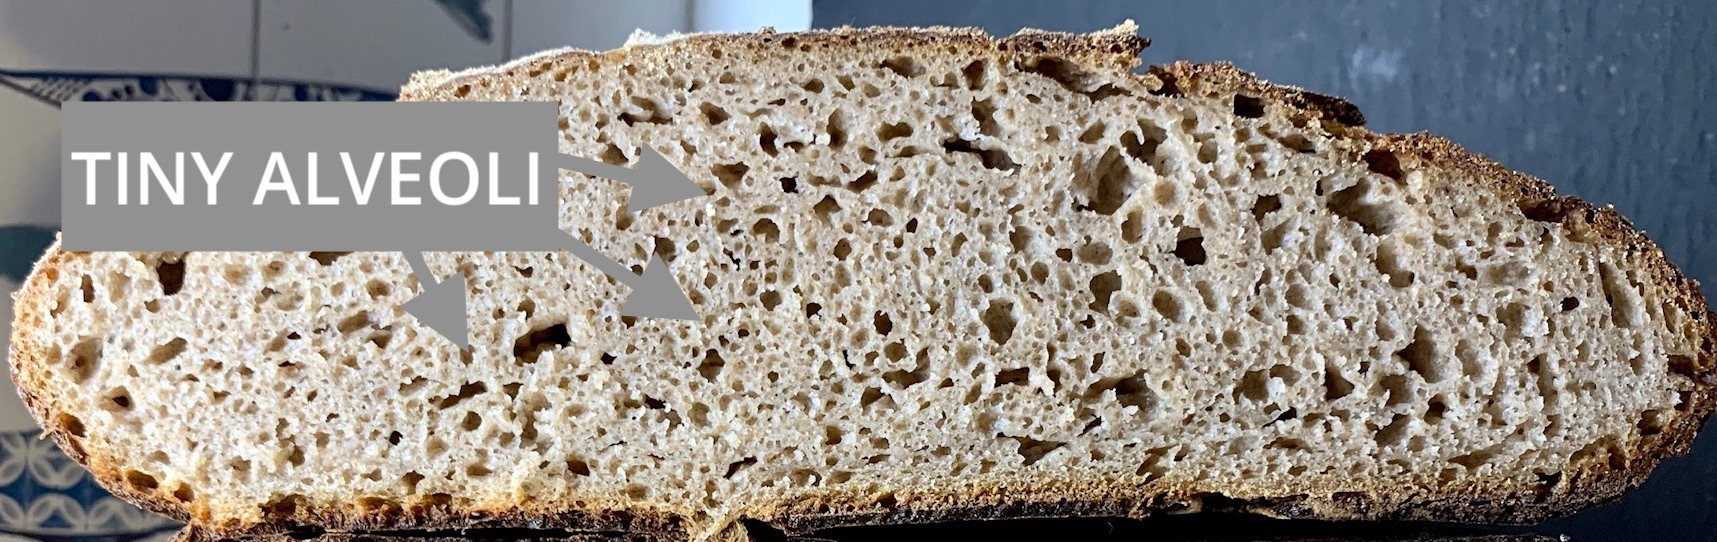
\includegraphics[width=\textwidth]{fermented-too-long}
  \caption{A relatively flat dough that has many tiny pockets of air.}
  \label{fig:fermented-too-long}
\end{figure}

When fermenting your dough for too long over time the protease enzyme starts to
break down the gluten of your flour. Furthermore the bacteria consumes the gluten
in a process called {\it proteolysis} \cite{raffaella+di+cagno}.
Bakers also refer to this process as {\it gluten rot}.
The gluten that normally is normally trapping the CO2 created
by the fermentation process of your microorganisms can no longer stay inside of
the dough. It disperses outward resulting in smaller alveoli in your crumb.
The bread itself tends to be very flat in the oven. Bakers often refer
to this style of bread as a {\it pancake}. The oven spring can be compared
to bread doughs made out of low gluten flour like Einkorn.

Your bread will feature a lot of acidity, a really strong distinctive tang. From
a taste perspective it might be a little bit too sour. From my own tests with family and
friends (n=15-20) I can say that this style of bread is typically
not as appreciated. However, me personally I really like the hearty strong taste.
It is excellent in combination with something
sweet or a soup.  From a consistency perspective it is no longer as fluffy as it could be.
The crumb might also taste a little bit gummy. That's because it has been broken down a lot
by the bacteria. Furthermore this style of bread has a significantly lower amount of gluten \cite{raffaella+di+cagno}
and is no longer comparable to raw flour, it's a fully fermented product.
You can compare it with a blue cheese that is almost lactose free.

When trying to work with the dough you will notice that suddenly the dough feels
very sticky. You can no longer properly shape and work the dough. When trying to
remove the dough from a banneton the dough flattens out very much. Furthermore
in many cases your dough might stick to the banneton. When beginning with baking
I would use a lot of rice flour in my banneton to dry out the surface of the dough a lot.
This way the dough wouldn't stick, despite being over fermented. However as it
turns out the stickiness issue has been my lack of understanding the fermentation
process. Now I never use rice-flour, except when trying to apply decorative scorings.
Properly managing fermentation results in a dough that is not sticky.

If you are noticing during a stretch and fold, or during shaping that your dough
is suddenly overly sticky, then the best option is to use a loaf pan. Simply take
your dough and toss it into a loaf pan. Wait until the dough mixture has increased
in size a bit again and then bake it. You will have a very well tasting sourdough
bread. If it's a bit too sour, you can just bake your dough for a longer period
of time to boil some of the acidity during the baking process. You can also use
your dough to setup a new starter and try again tomorrow. Lastly if you are hungry
you can simply pour some of your dough directly into a heated pan with a bit of
oil. You will be making delicious sourdough flat breads.

To fix issues related to overfermentation you need to stop the fermentation process
earlier. What I like to do is to extract a small fermentation probe from my dough.
Depending on the volume increase of this probe I can mostly judge when my fermentation
is finished. Try to start with a 25 percent volume increase of your main dough or sample.
Depending on how much gluten your flour has, you can ferment for a longer period of time.
With a strong flour featuring a 14-15 percent protein you should be able to safely
ferment until a 100 percent size increase. This however also happens on your
sourdough starter's composition of yeast and bacteria. The more bacterial fermentation
the faster your dough structure breaks down. Frequent feedings of your sourdough
starter will improve the yeast activity. Furthermore a stiff sourdough starter
might be a good solution too. The enhanced yeast activity will result in a more fluffy
dough with less bacterial activity. A better yeast activity also will result
in less acidity in your final bread. If you are a chaser of a very strong tangy
flavor profile then a stronger flour with more gluten will help.


\subsection{Underfermented}

\begin{figure}
  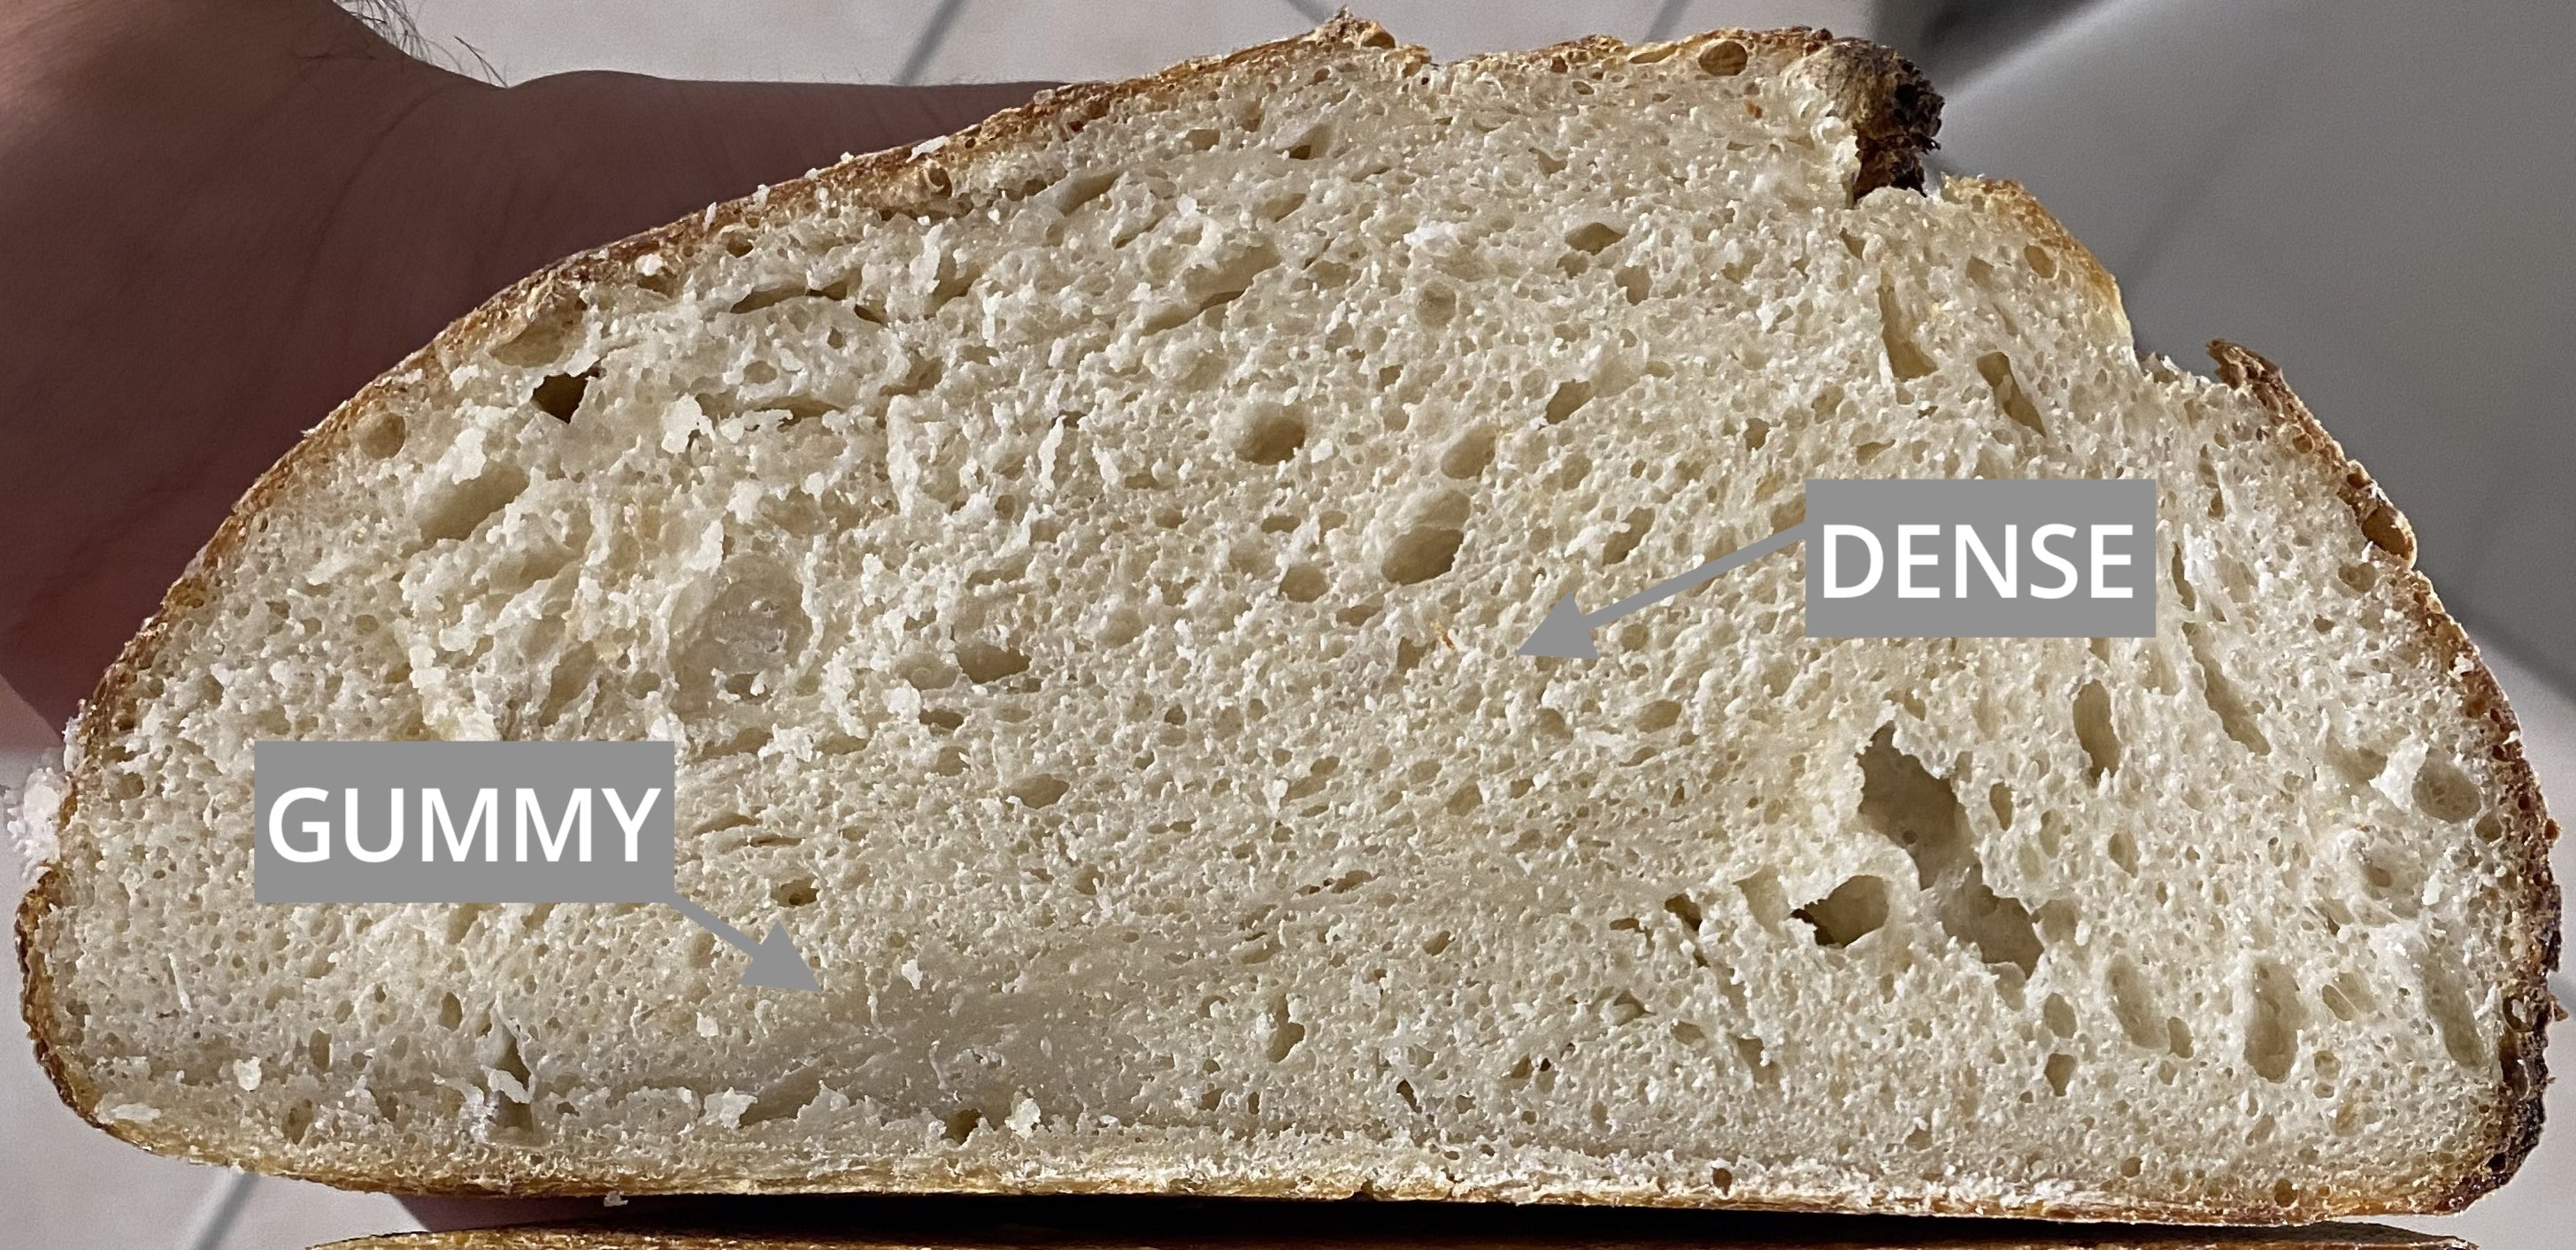
\includegraphics[width=\textwidth]{fermented-too-short-underbaked}
  \caption{A dense dough featuring a gummy not fully gelatinized area.
  The picture has been provided by Midori from our community discord server.}
  \label{fig:fermented-too-short-underbaked}
\end{figure}

This defect is also commonly referred to as {\it underproofed}. However underproofed
is not a good term as it only refers to having a too short period of time in the final
proofing stage of the bread making process. If you were to directly bake your bread
after a successful bulk fermentation stage you would not achieve this defect.
Proofing will make your dough a bit more extensible and allows your sourdough
to inflate the dough a bit more. When faced with an underfermented bread you
already did something wrong during the bulk fermentation stage, or maybe also
even before that with your sourdough starter.

A typical underfermented dough has very large pockets of air and is partially
wet and gummy in some areas of the dough. The large pockets can be compared
to making a non-leavened wheat or corn tortilla. As you bake the dough in your pan
the water slowly starts to evaporate. The gas is trapped in the structure of the dough
and will create pockets. In case of a tortilla this is the desired behavior.
But when you observe this process in a larger dough you will create several
super alveoli. The water evaporates and the first alveoli form. Then at some point
the starch starts to gelatinize and becomes solid. This happens first inside of the pockets
as the interior heats up faster compared to the rest of the dough. Once all the starch
has gelatinized the alveoli holds its shape and no longer expands. During this
process other parts of the bread dough are pushed outwards. That's why an underfermented
dough sometimes even features an ear during the baking process. This
is also commonly referred to as a {\it fool's crumb}. You are excited about an ear which
can be quite hard to achieve. Plus you might think you finally created some big pockets
of air in your crumb. But in reality you fermented for a too short period
of time.

\begin{figure}
  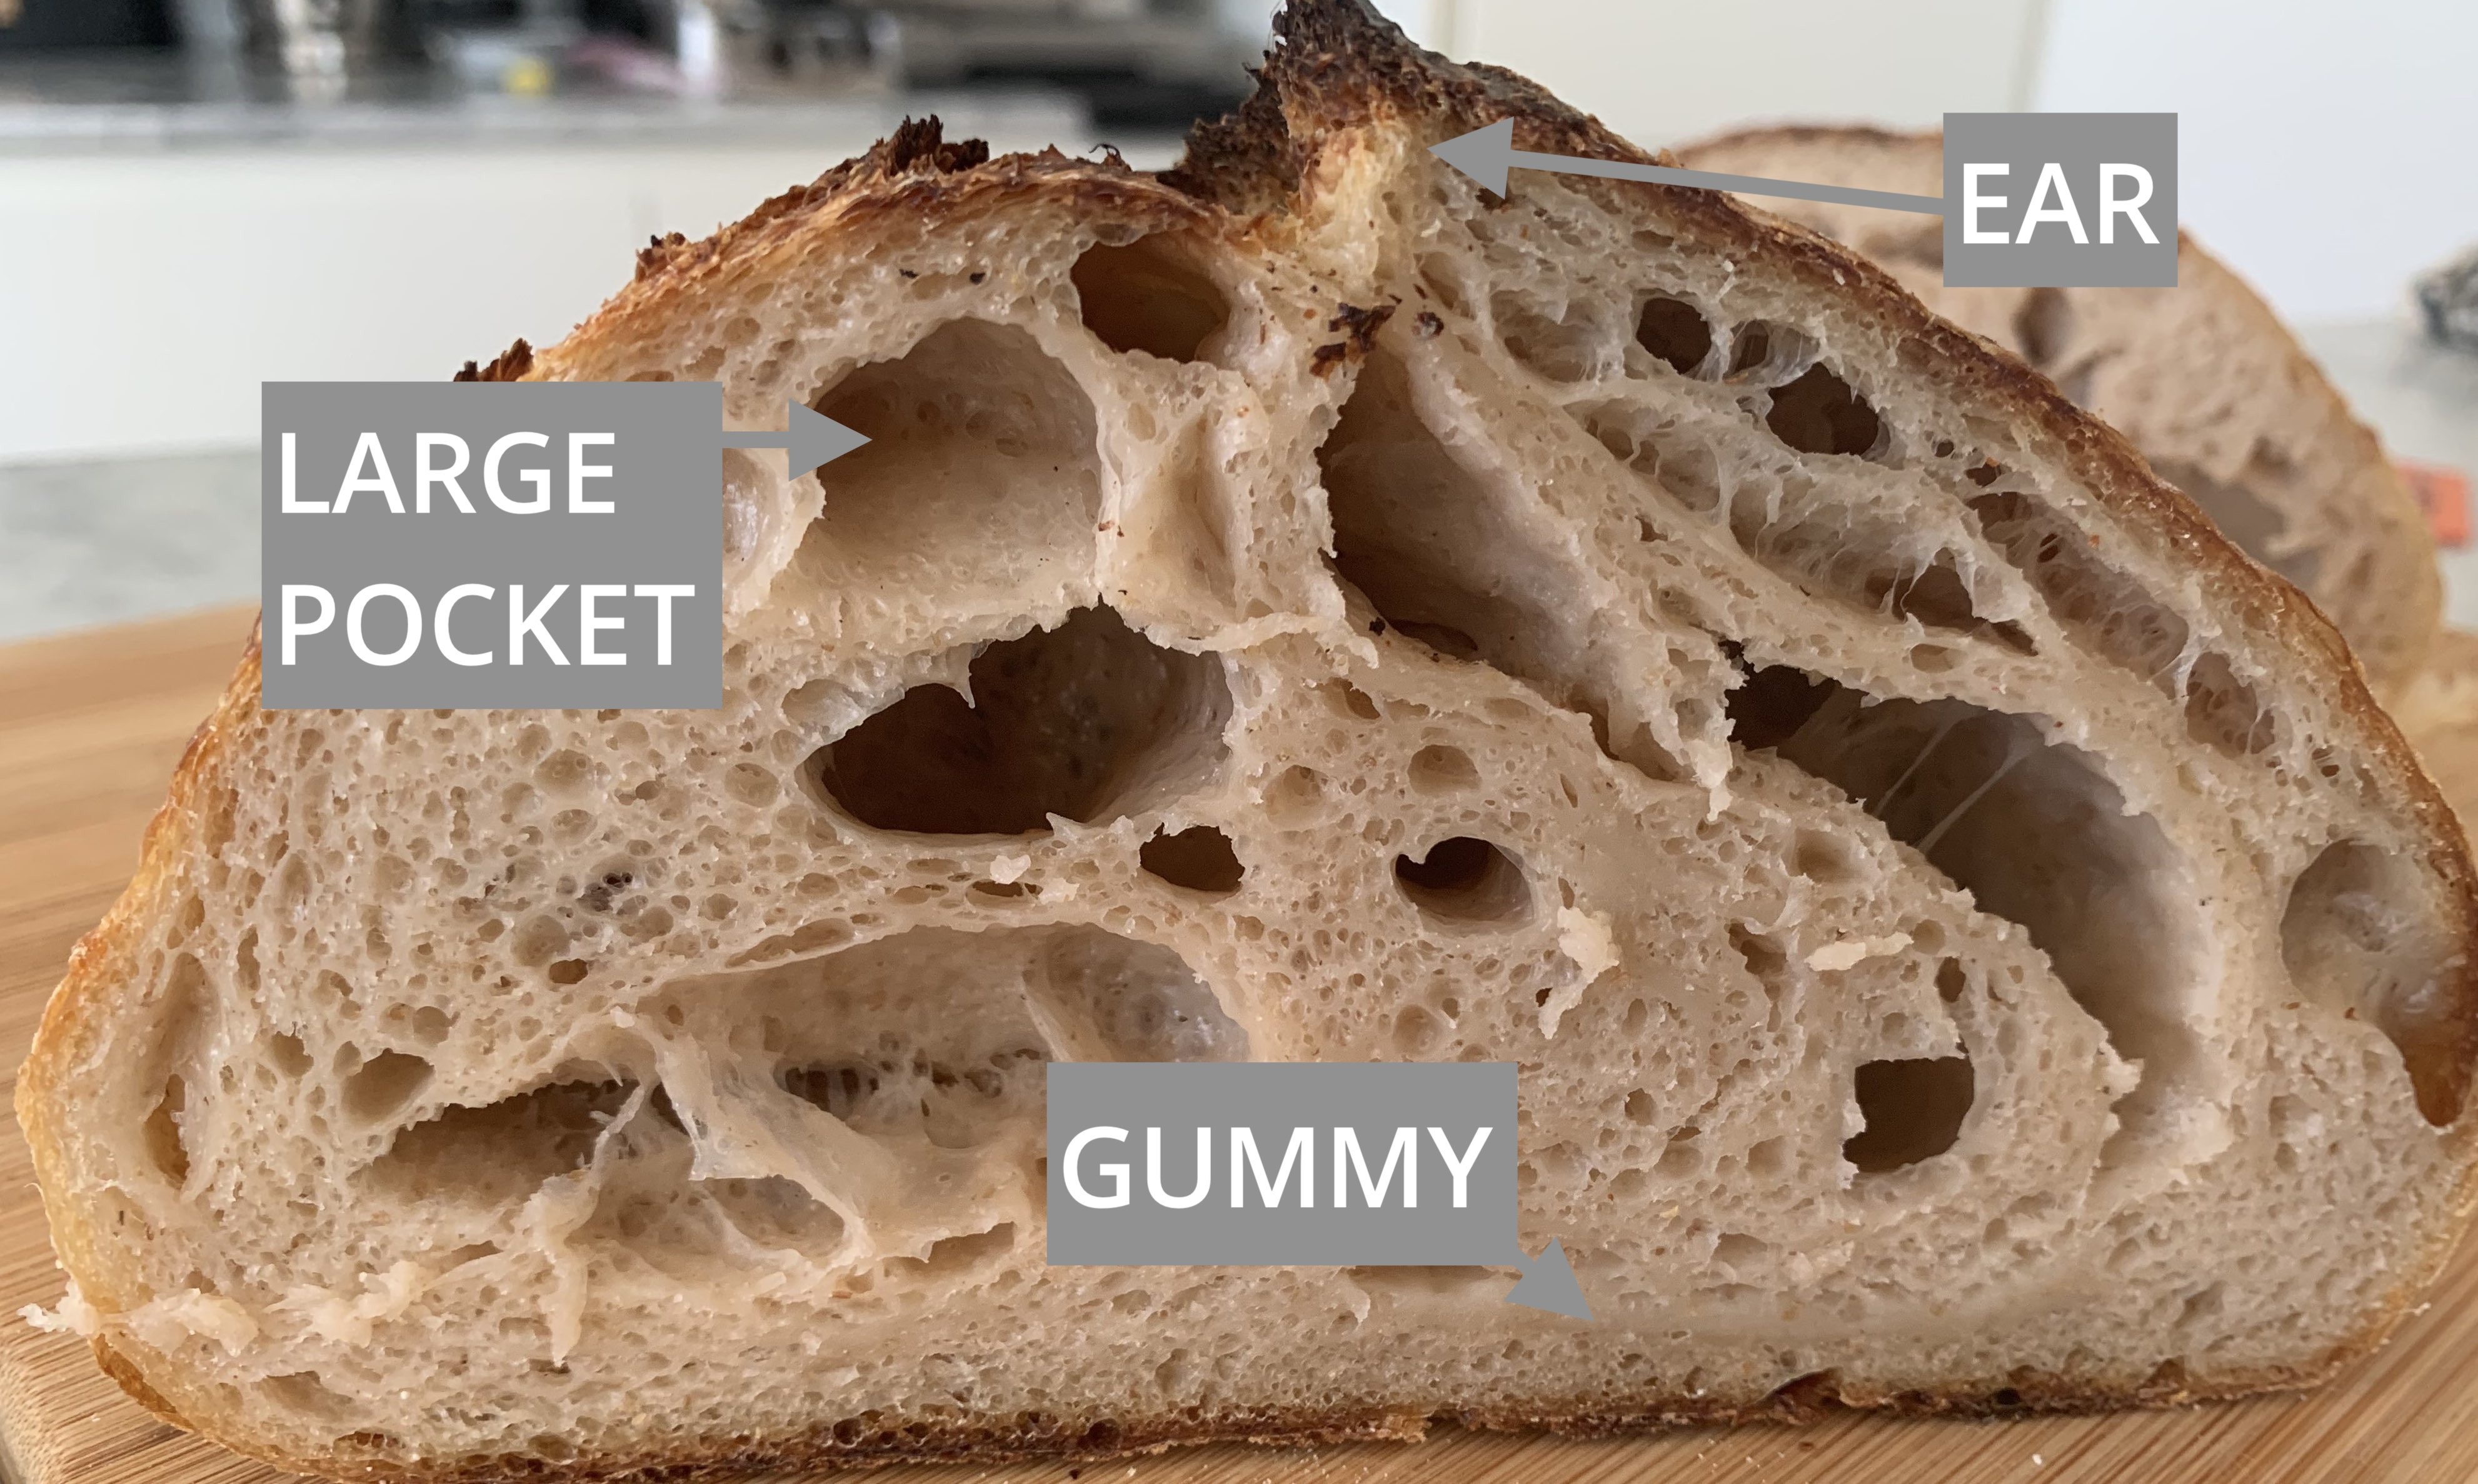
\includegraphics[width=\textwidth]{fools-crumb}
  \caption{A typical example of a fool's crumb featuring an ear and several overly
  large alveoli. The picture has been provided by Rochelle from our
  community discord server.}
  \label{fools-crumb}
\end{figure}

In a properly fermented dough the alveoli help with the heat transfer throughout the dough.
From within the tiny many fermentation induced pockets the starch gelatinizes. With
an underfermented dough this heat transfer does not properly work. Because of that
you sometimes have areas which look like raw dough. Bakers refer to this as a very
gummy structure sometimes. Baking your dough for a longer period of time would also properly
gelatinize the starch in these areas. However, then other parts of your bread
might be baked too long.

To fix issues related to underfermentation you simply have to ferment your dough
for a longer period of time. Now there is an upper limit to fermentation time
as your flour breaks down the moment it is in contact with water. That's why it
might be a good idea to simply speed up your fermentation process. As a rough
figure, I try to aim for a bulk fermentation time of around 8-12 hours typically.
To achieve that you can try to make your sourdough starter more active.  This can be done
by feeding your starter daily over several days. Use the same ratio as you would
do for your main bread dough. Assuming you use 20 percent starter calculated on the flour,
use a 1:5:5 ratio to feed your starter. That would be 10 grams of existing starter,
50 grams of flour, 50 grams of water for instance. To boost your yeast even more you can
consider making a stiff sourdough starter. The stiff sourdough starter will
boost your yeast activity. The bacteria produces mostly acid. The more acidity
is piled up, the less active your yeast is. The stiff sourdough starter
enables you to start your dough's fermentation with yeast dominated activity.


\subsection{Not enough dough strength}

\begin{figure}
  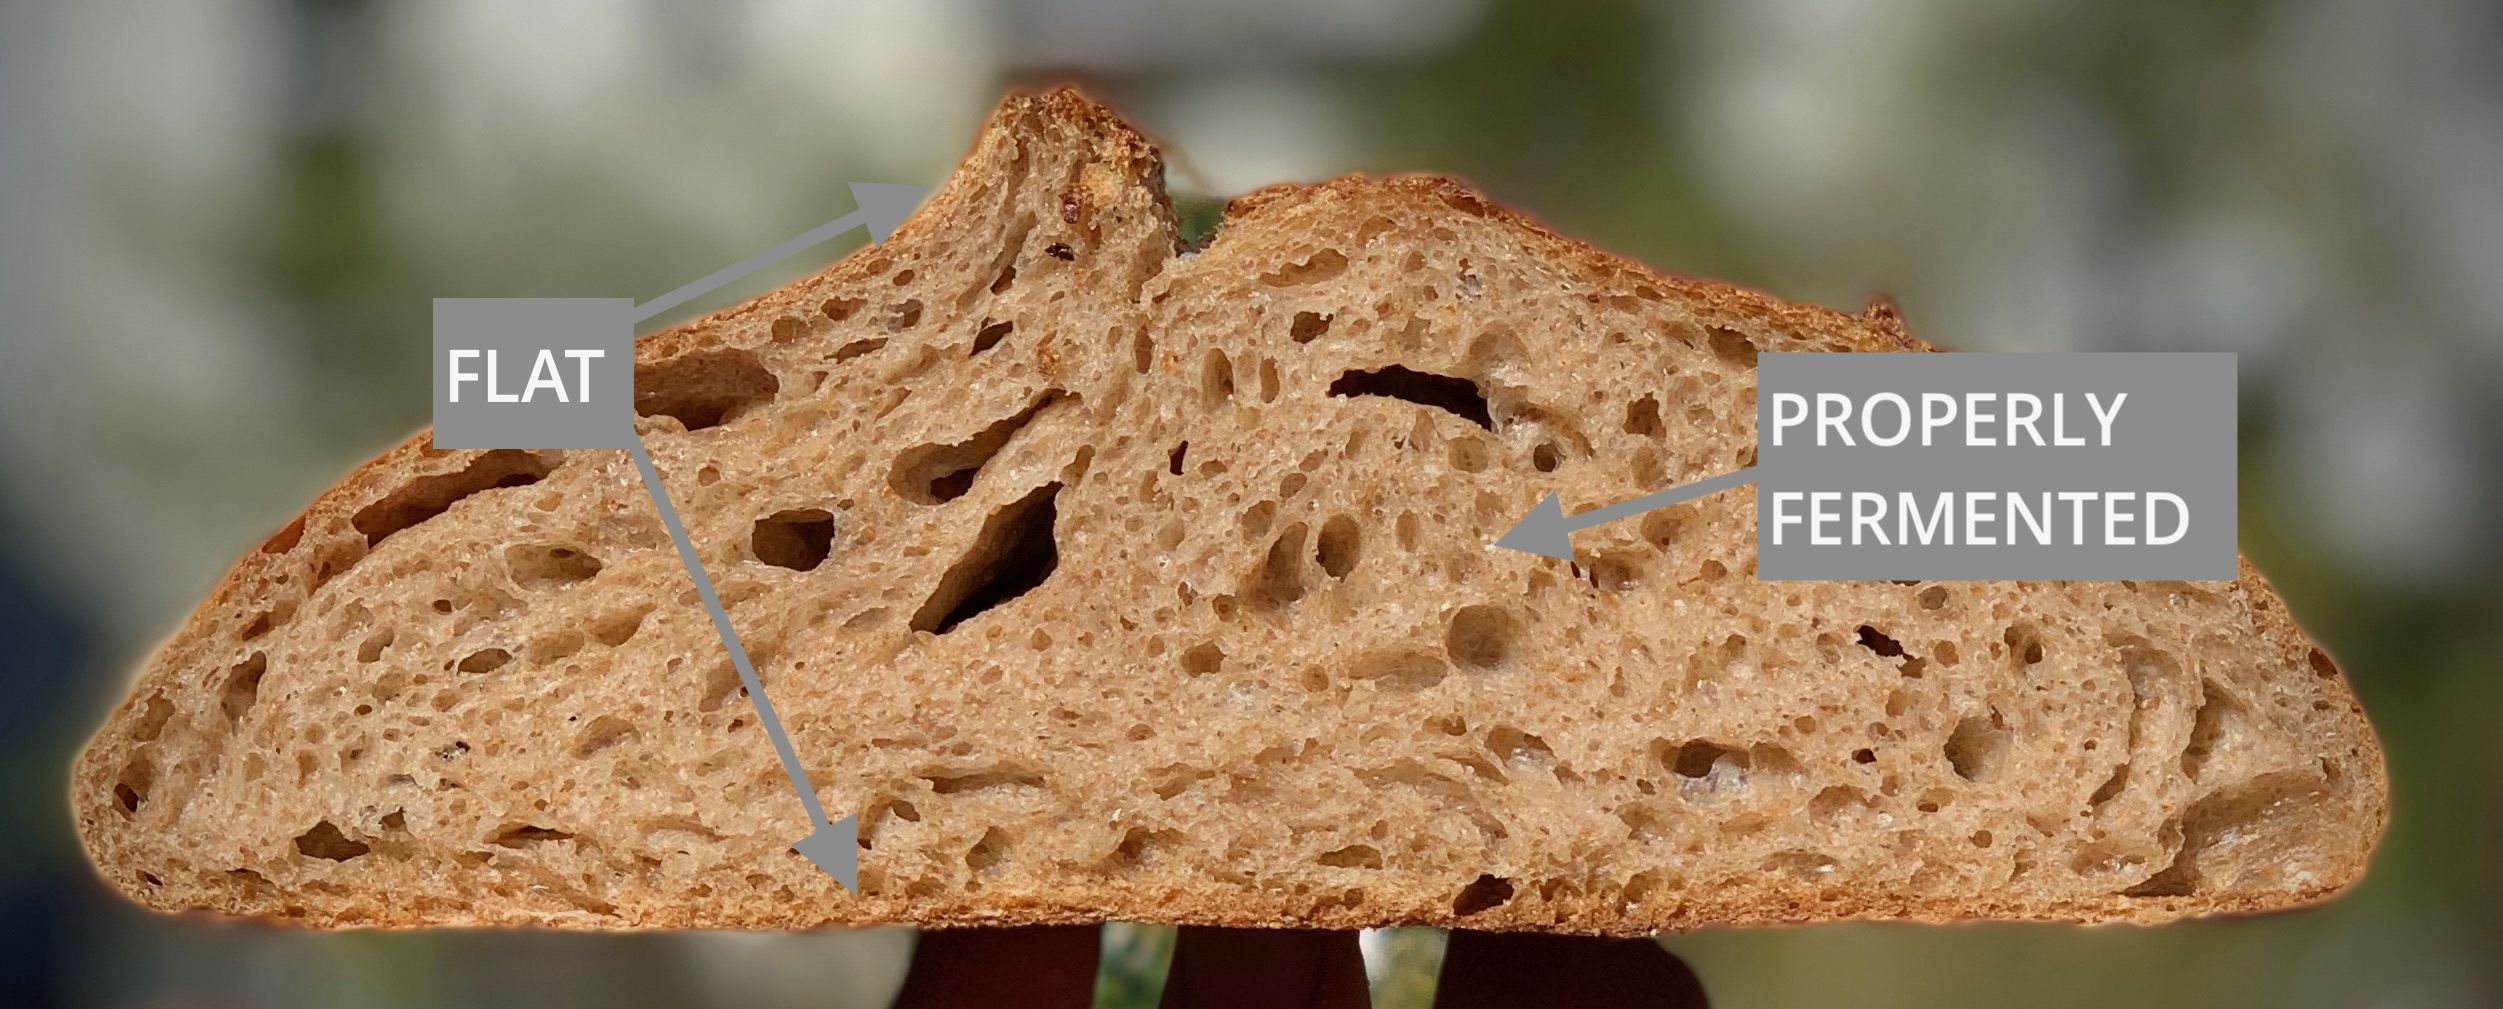
\includegraphics[width=\textwidth]{flat-bread}
  \caption{A very flat bread without enough dough strength.}
  \label{flat-bread}
\end{figure}

When a dough flattens out quite a lot during the baking process chances are
that you did not create enough dough strength. This means your gluten matrix
hasn't been developed properly. Your dough is too extensible and flattens out
mostly rather than springing upwards in the oven. This can also happen if you
proofed your dough for too long. Over time the gluten relaxes and your dough
becomes more and more extensible. You can observe the gluten relaxing behavior
too when making a pizza pie. Directly after shaping your dough balls it's very hard to shape
the pizza pie. If you wait for 30-90 minutes stretching the dough becomes a lot easier.

The easiest way to fix this is probably to knead your dough more at the start. To simplify
things consider using less water for your flour too. This will result in a more elastic dough
right away. This concept is commonly used for no-knead style sourdough.  Alternatively you
can also perform more stretch and folds during the bulk fermentation process. Each
stretch and fold will help to strengthen the gluten matrix and make a more elastic dough.
The last option to fix a dough with too little dough strength is to shape your dough tighter.

\subsection{Baked too hot}

\begin{figure}
  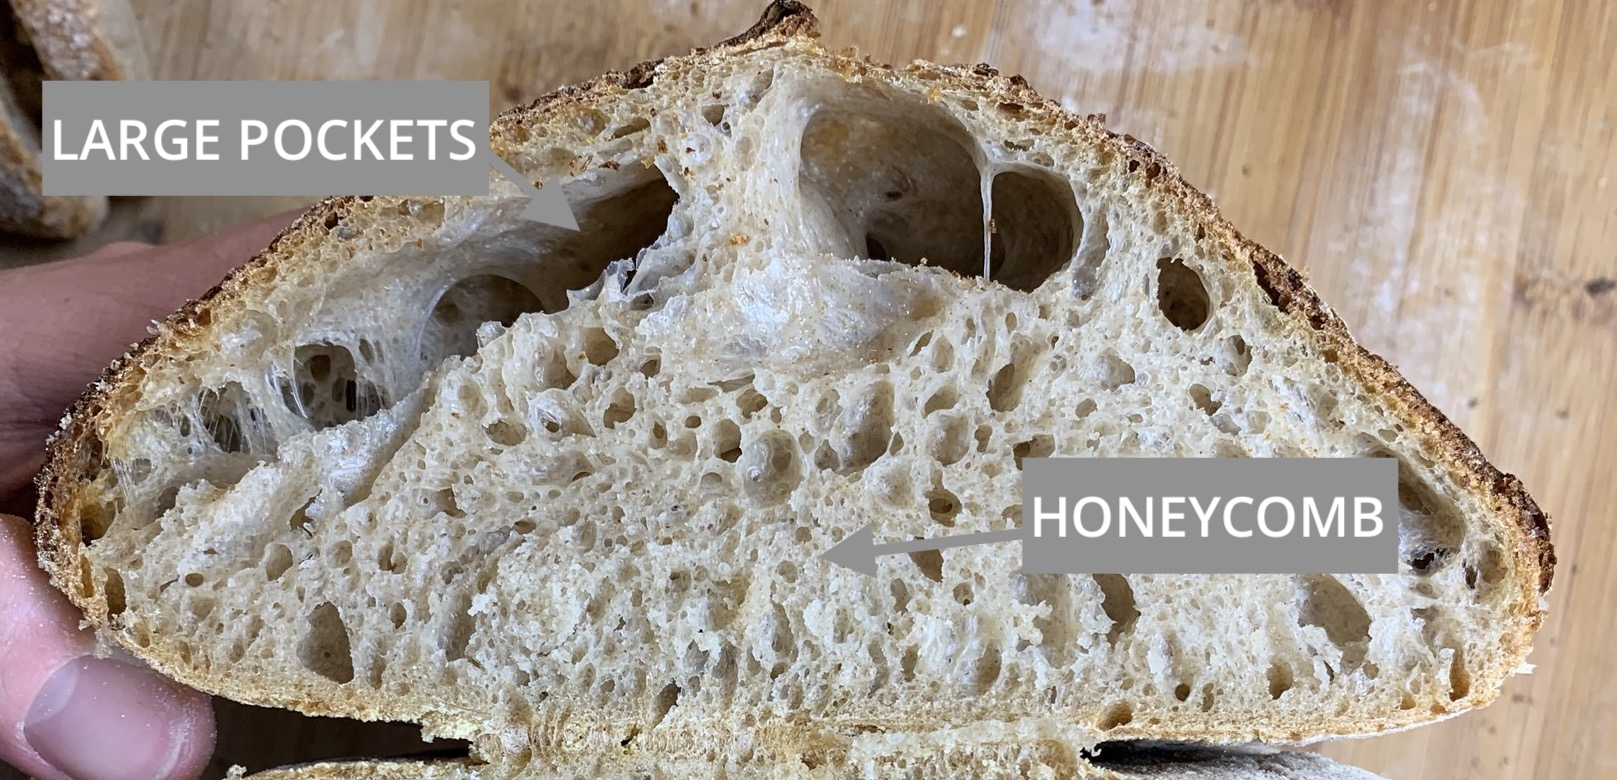
\includegraphics[width=\textwidth]{baked-too-hot-v2}
  \caption{A bread with very large alveoli close to the crust}
  \label{baked-too-hot}
\end{figure}

This is a common mistake that has happened to me a lot. When you bake your dough
at a too hot temperature you block your dough's expansion. The starch gelatinizes
and becomes more and more solid. At around 140°C (284°F) the maillard reaction
starts to completely thicken your bread dough's crust. This is similar to baking
your bread dough without steam. As the internal dough's temperature heats up
more and more water evaporates, gas expands and the dough is being pushed upwards.
Once the dough reaches the crust it can no longer expand. The alveoli merge
into larger structures close to the surface of the dough. By baking too hot
you are not achieving the ear which adds extra flavor. Furthermore your crumb
is not as fluffy as it could be by restricting its expansion capabilities.

If you have an extensible dough with high hydration baking too cold will result
in the dough flattening out quite a lot. The gelatinization of the starch is
essential for the dough to hold it's structure. After conducting several
experiments it seems that my sweet spot for maximum oven spring seems to be
at around 230°C (446°F). Test the temperature of your oven, because in several
cases the displayed temperature might not match the actual temperature of your
oven \cite{too+hot+baking}. Make sure to turn off the fan of your oven. Most
home ovens are designed to vent the steam as fast as possible. If you can not
turn the fan off, consider using a dutch oven.

\subsection{Baked with too little steam}

\begin{figure}[h]
  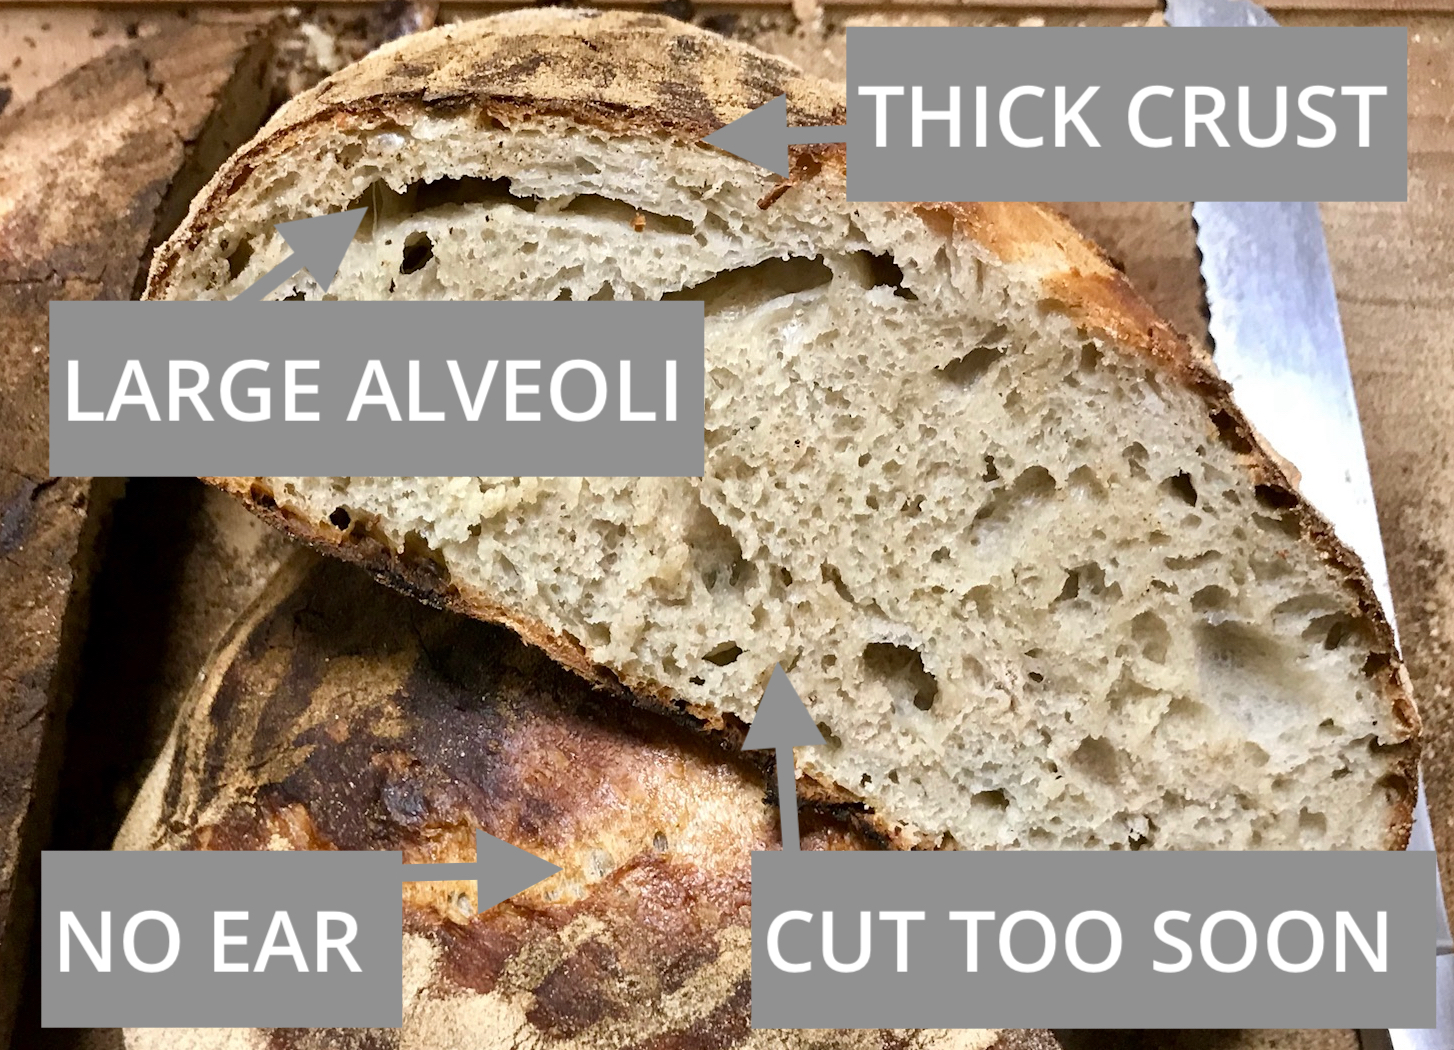
\includegraphics[width=\textwidth]{no-steam}
  \caption{One of my earlier breads that I baked at a friend's place where
  I couldn't steam the dough properly}
  \label{no-steam}
\end{figure}

Similarly to baking too hot when baking without enough steam your dough's crust
forms too quickly. It's hard to spot the difference between the two mistakes.
I typically first ask about the temperature and then about the steaming technique
to determine what might be wrong with the baking process. Too little steam can
typically be spotted by having a thick crust around all around your dough paired
with large alveoli towards the edges.

The steam essentially prevents the maillard reaction from happening too quickly
on your crust. That's why steaming during the first stages of the bake is so important.
The steam keeps the temperature of your crust close to around 100°C (212°F). Achieving steam
can be done by using a dutch oven, an inverted tray and or a bowl of boiling water.
You might also have an oven with a built-in steam functionality. All the methods work,
it depends on what you have at hand. My default go-to method is an inverted
tray on top of my dough, paired with a bowl full of boiling water towards the bottom
of the oven.

\begin{figure}
  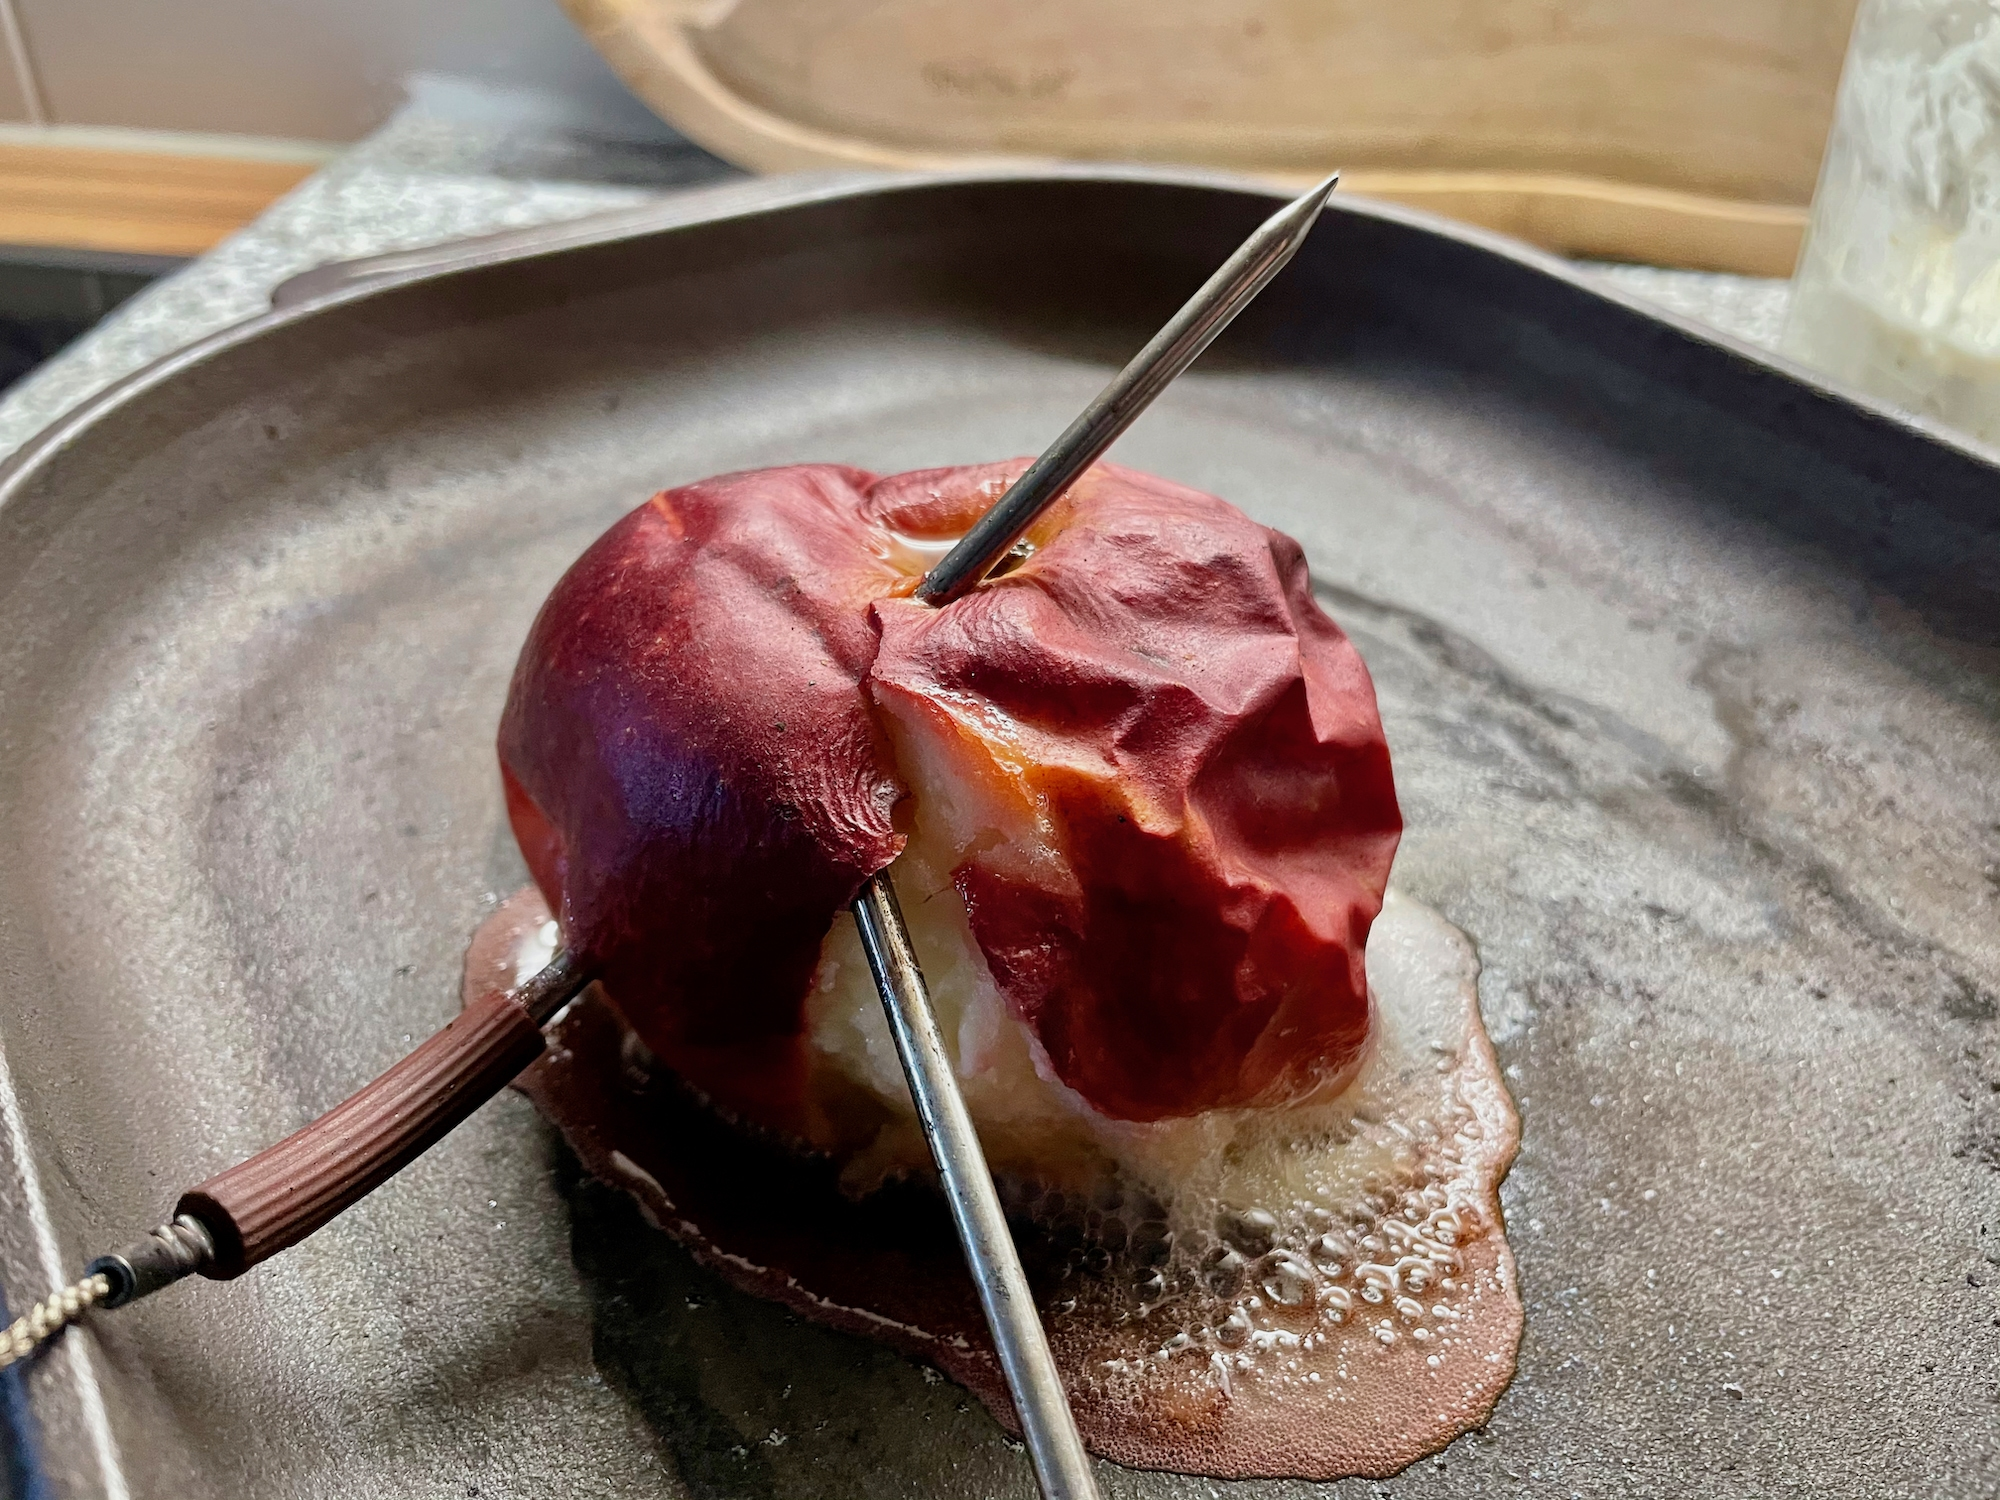
\includegraphics[width=\textwidth]{apple-experiment-temperatures}
  \caption{An apple with 2 probes to measure ambient
  and surface temperatures of several steaming techniques
  in a dutch oven.}
  \label{apple-experiment-temperatures}
\end{figure}

Now there can also be too much steam. For this I tested using a dutch oven paired with large ice
cubes to provide additional steam. The temperature of my dough's surface would directly
jump close to 100°C. The steam contains more energy and can thus through convection
heat up the surface of your dough faster. I tested this by using an apple inside of
a dutch oven. Then I would use a barbecue thermometer with a probe directly at the surface.
I would then change the steaming methods to plot how quickly the temperature
close to the surface of the dough changes. I tried to use an ice cube inside of a preheated
dutch oven, a preheated dutch oven, a preheated dutch oven with spritzes
of water on the apple's surface, a non preheated dutch oven where I would only preheat
the bottom part. The experiment then showed that the ice-cube method would heat up
the surface of the apple a lot quicker. When replicating this with a bread dough
I would achieve less oven spring.

\begin{figure}[h]
  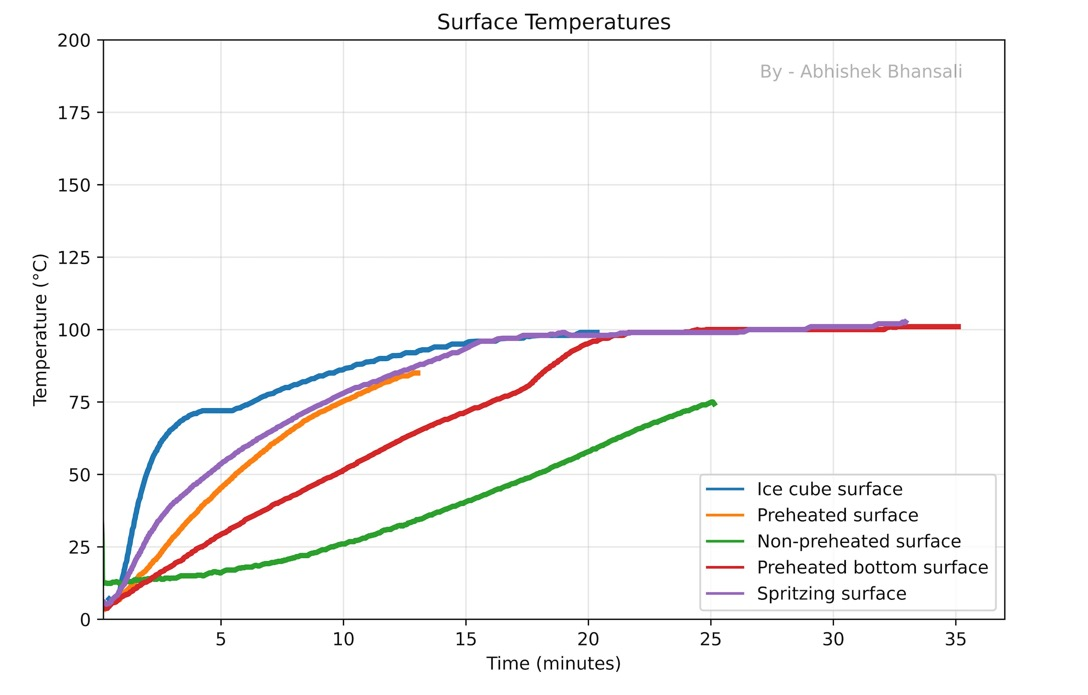
\includegraphics[width=\textwidth]{apple-experiment-surface-temperatures}
  \caption{A chart showing how the temperature of the surface
  of the apple changes with different steaming techniques.}
  \label{apple-experiment-surface-temperatures}
\end{figure}

\begin{figure}[h]
  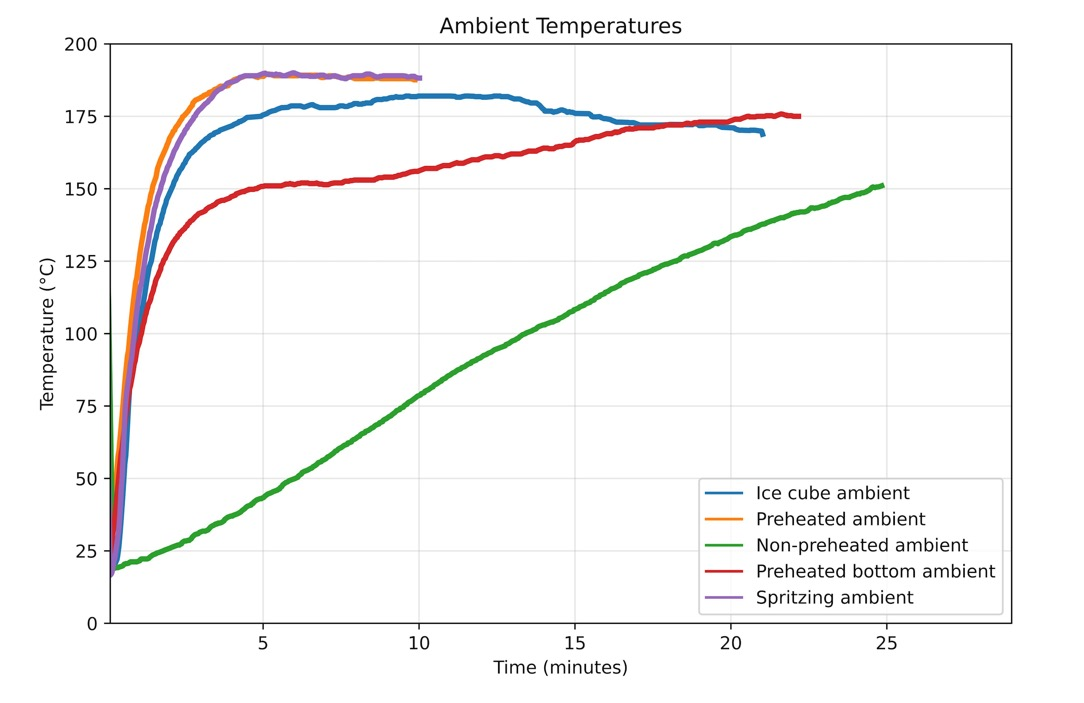
\includegraphics[width=\textwidth]{apple-experiment-ambient-temperatures}
  \caption{This figure shows how the ambient temperatures inside of the
  dutch oven change depending on the steaming technique that is used.}
  \label{apple-experiment-ambient-temperatures}
\end{figure}

Generally though achieving too much steam is relatively challenging. I could only
commit this mistake when using a dutch oven as steaming method paired with relatively
large ice cubes. After talking with other bakers using the same dutch oven, it seems
that mine (around 80g) were 4 times as heavy as the ones other bakers would use (20g)
\section{Baking in the tropics}

Depending on the temperature your fermentation speed adapts.
In a warmer environment everything is faster. In a colder
environment everything is slower.

This includes the speed at which your sourdough ferments
the dough but also the speed of enzymatic reactions. The
amylase and protease enzymes work faster, making more
sugars available and degrading the gluten proteins.

At around 22°C in my kitchen my bulk fermentation is ready
after around 10 hours. I am using around 20 percent of sourdough
starter based on the flour. In summer times the temperatures
in my kitchen sometimes increase to 25°C. In that case
I am reducing the sourdough starter to around 10 percent.
If I wouldn't do that my fermentation would be done after
around 4-7 hours. The problem is that the dough is quite
unstable when fermenting at this high speed. This means
that you are easily running into issues of overfermentation.
Finding the perfect sweet spot between fermenting enough
and not too much is becoming much harder. Normally you might
have a time window of 1 hour. But at the rapid speed it
might be reduced to a time window of 20 minutes. Now at
30°C ambient temperature things are way faster. Your bulk
fermentation might be complete in 2-4 hours when using
10-20 percent starter. Proofing your dough in the fridge
becomes almost impossible. As your dough cools down in the
fridge the fermentation also slows down. However cooling the
dough down from 30°C to 4-6°C in your fridge takes much
longer. Your dough is much more active compared to a dough
that starts at a temperature of 20-25°C. You might
end up overproofing your dough if you leave it overnight
in the fridge.

That's why I recommend that you reduce the amount of starter
that you use in the tropics to something at around 1-5 percent
based on the flour. This will slow down the fermentation
process significantly and provides you a bigger window
of time. Try to aim for an overall bulk fermentation of at
least 8-10 hours. Reduce the amount of starter to get there.

When making a dough try to use the same water temperature
as your ambient temperature. Assuming that the temperature
will climb to 30°C, try to start your dough directly
with 30°C water. This means that you can carefully rely on
a small fermentation probe that visualizes your fermentation
progress. The probe only works reliably if your dough temperature
is equal to your ambient temperature. Else the sample heats
up or cools down faster. So tread carefully when using
the sample in this case. It's always better to stop
the fermentation a little too early rather than too late.
Stretch and folds during the bulk fermentation
will help you to develop a better look and feel for
the dough. An expensive but possibly useful tool
could be a pH meter that allows you to perfectly
measure how much acidity has been created by the
lactic and acetic acid bacteria. In this case measure
the pH repeatedly and figure out a value that works
for your sourdough. In my case I tend to end bulk
fermentation at a pH of around 4.1. Please don't just
follow my pH value, it's very individual. Keep measuring
with different doughs to find out a value that works for you.

\section{My bread stays flat}

A flat bread is in most cases related to your gluten
network breaking down fully. This is not bad, this
means you are eating a fully fermented food. However
from a taste and consistency perspective it might be
that your bread tastes too sour, or is not fluffy anymore.
Please also note that you can only make bread with
great oven spring when making wheat based doughs. When
starting with this hobby I always wondered why my rye
breads would turn out so flat. Rye has gluten yes, but
small particles called {\it hemicelluloses} (arabinoxylan and beta-glucan) \cite{rye-defects}.
prevent the dough from developing a gluten network like you can
do with wheat. Your efforts are in vain, your dough will
stay flat. Only spelt and wheat based doughs have the capability
to retain the CO2 created by the fermentation.

In most cases something is probably off with your
sourdough starter. This very often happens when the starter
is still relatively young and hasn't yet matured
at fermenting flour. Over time your sourdough
starter is going to become better and better at fermenting
flour. Keep your sourdough starter at room temperature
and then apply daily feedings with a 1:5:5 ratio.
This would be 1 part old starter, 5 parts flour,
5 parts water. This allows you to achieve a better
balance of yeast and bacteria in your sourdough.
Even better could be the use of a stiff sourdough
starter. The stiff sourdough starter boosts
the yeast part of your starter. This allows you
to have less bacterial fermentation, resulting
in a stronger gluten network towards the end
of the fermentation \cite{stiff+starter}. Please
also refer to the section ~\ref{sec:overfermented-dough} where
I explained more about overfermented doughs.

\begin{figure}[!htb]
  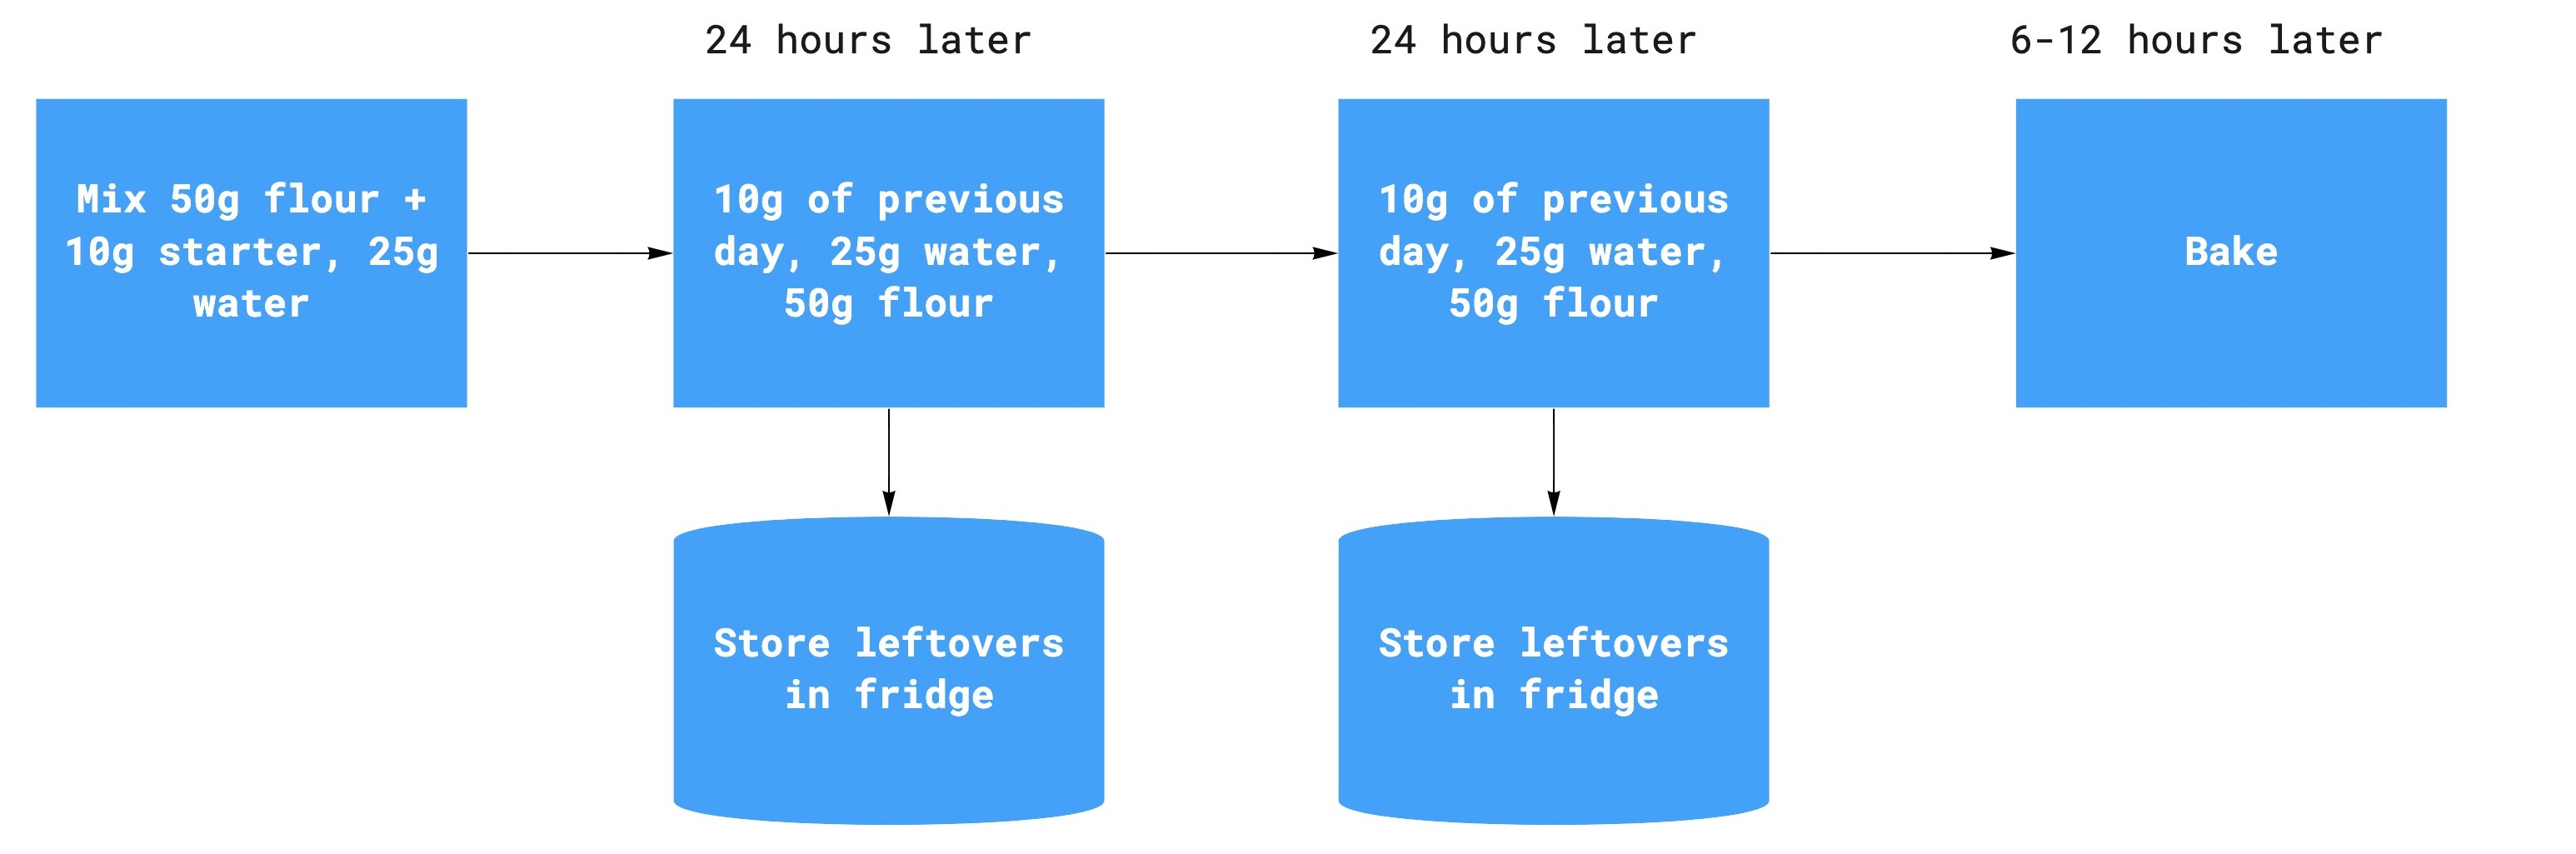
\includegraphics[width=\textwidth]{stiff-starter-conversion}
  \caption{The process to convert your starter into a stiff starter.}
  \label{fig:stiff-starter-conversion}
\end{figure}

Furthermore a stronger flour containing more gluten
will help you to push the fermentation further. This
is because your flour contains more gluten and will
take longer to be broken down by your bacteria. Ultimately
if fermented for too long your dough is also going
to be broken down and will become sticky and flat.

To debug whether the excess bacterial fermentation is the issue,
simply taste your dough. Does it taste very sour? If yes,
that's a good indicator. When working the dough, does it
suddenly become very sticky after a few hours? That's a
another good indicator. Please also use your nose to note
the smell of the dough. It shouldn't be too pungent.

\section{I want more tang in my bread}

To achieve more tang in your sourdough bread you have
to ferment your dough for a longer period of time.
Over time the bacteria will metabolize most of the
ethanol created by the yeast in your dough. The bacteria
mostly produces lactic and acetic acid. Lactic acid
is chemically more sour than acetic acid but sometimes
not achieved as sour. In most cases a longer fermentation
is what you want. You will either need to utilize a loaf
pan to make your dough or use a flour that can withstand
a long fermentation period. A flour like this is typically
called a {\it strong flour}. Stronger flours tend
to be from wheat varieties that have be grown in more
sunny conditions. Because of that stronger flours tend
to be more expensive. For freestanding loaves I recommend
to use a flour that contains at least 12 percent protein.
Generally the more protein the longer you can ferment your dough.

Another option to achieve a more sour flavor could be to
use a starter that produces more acetic acid. Acetic acid
bacteria tend to be more common in rye starters (source needed).
Chemically the acetic acid isn't as sour, but when tasting
it will seem more sour. Make sure to use a starter that is at
a hydration of around 100 percent. Acetic acid production
requires oxygen. A too liquid starter tends to favor lactic
acid production because the flour is submerged in water, no
oxygen can reach the fermentation after a while.

\begin{figure}[!htb]
  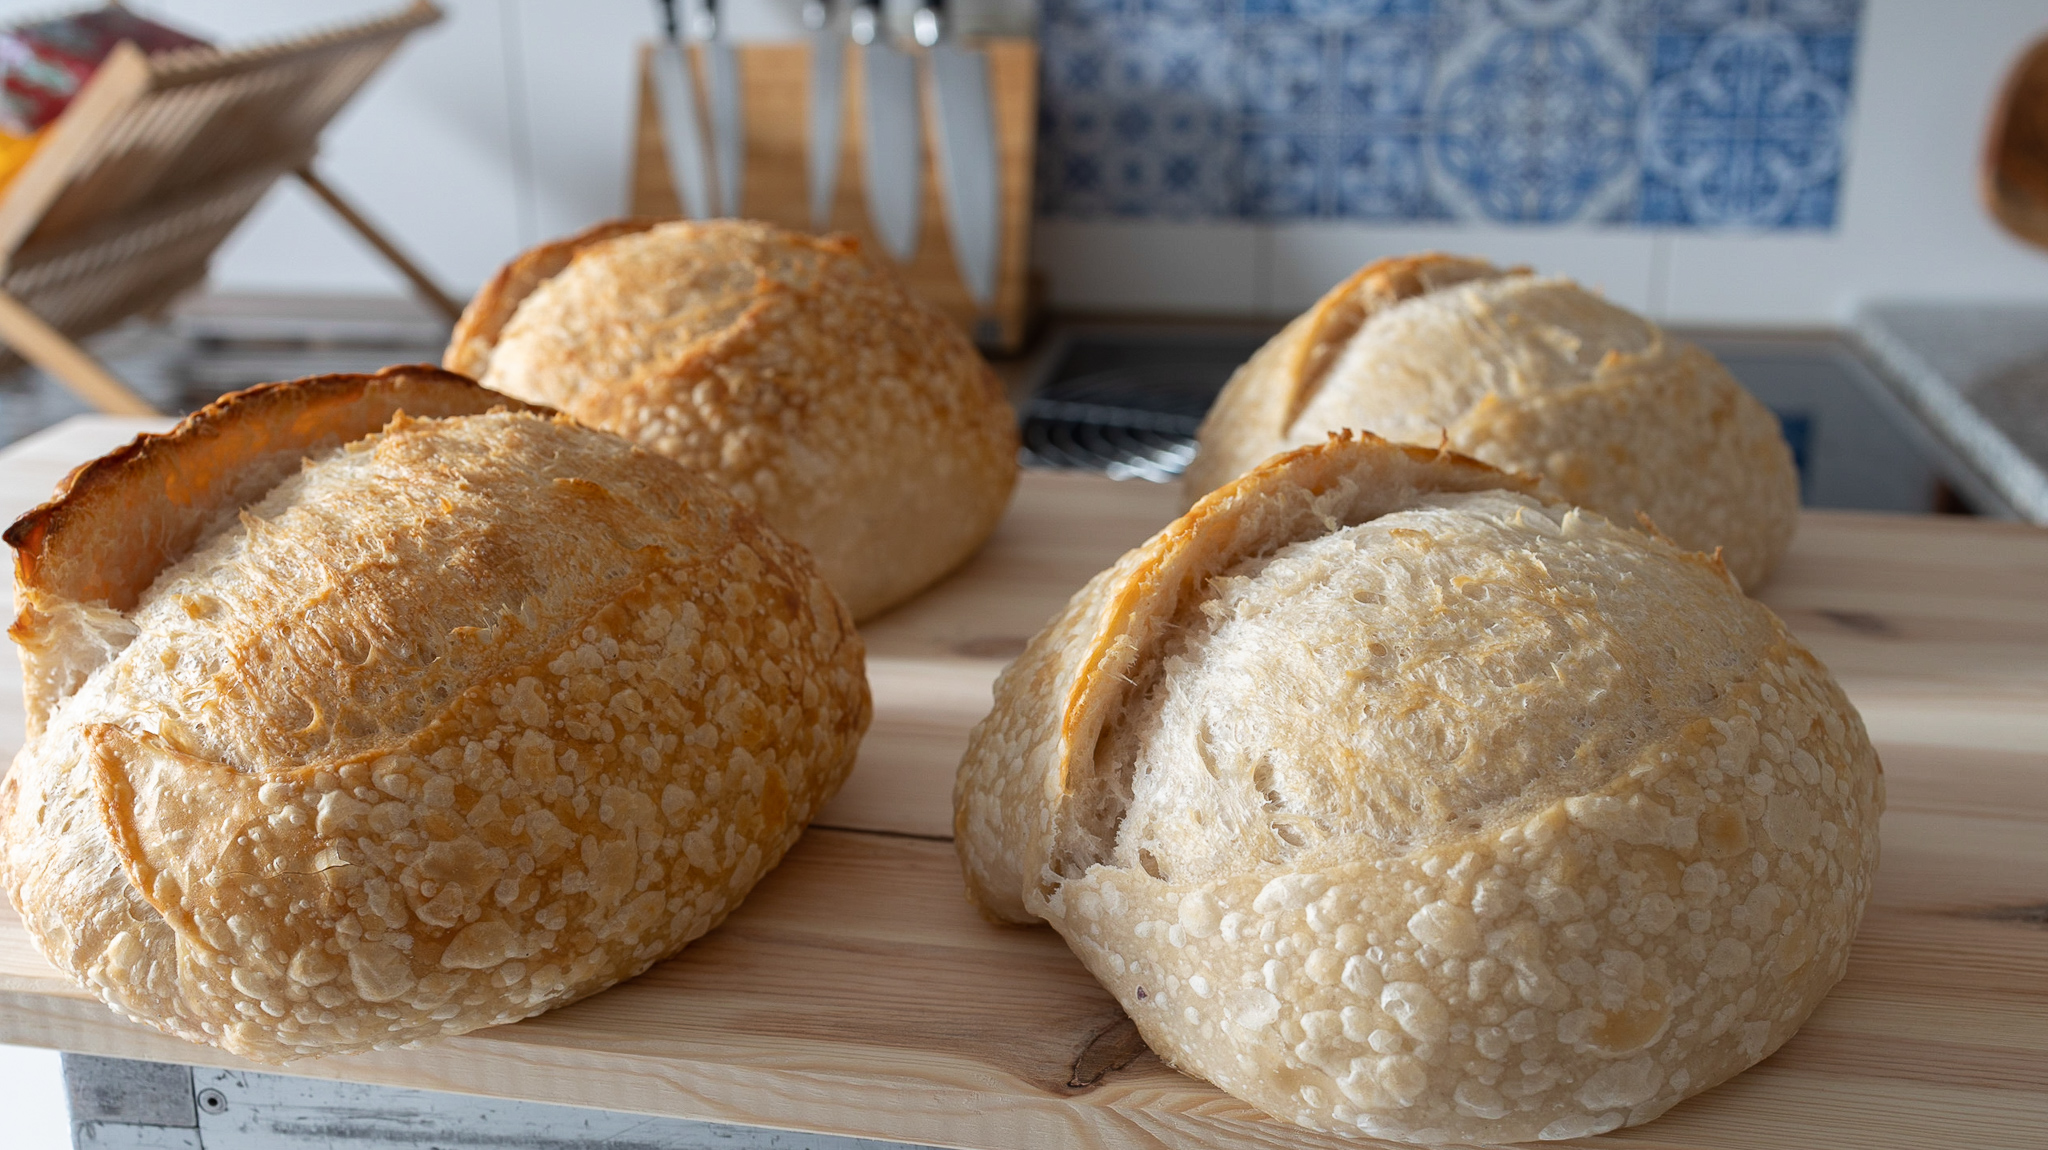
\includegraphics[width=\textwidth]{parbaked-bread.jpg}
  \caption{A half-baked bread, known as "parbaked".}
  \label{fig:parbaked-bread}
\end{figure}

Another more easier option could be to bake your sourdough
twice. I have observed this when shipping bread for my micro
bakery. The idea was to bake my bread for around 30 minutes
until it's sterilized, let it cool down and then ship it
to customers. Once you receive it you just bake it again
for another 20-30 minutes to achieve the desired crust and
then you can eat it. Some of the customers reported a very sour
tasting bread. After investigating a bit more it became
crystal clear. By baking the bread twice you don't boil
as much of the acid during the baking process. Water
evaporates at around 100°C while acetic acid boils at
118°C and lactic acid at 122°c. After baking for 30 minutes
at around 230°C some of the water has started to evaporate,
but not all the acid yet. If you were to continue to bake more
and more of the acid would start to evaporate. Now if you were
to stop baking after 30 minutes, you would typically have reached
a core temperature of around 95°C. Your dough would need
to be cooled down again to room temperature. The crust would
still be quite pale. Then A couple of hours later you start
to bake your dough again. Your crust would become nice and
dark featuring delicious aroma. The aroma is coming from the
maillard reaction. However the core of your dough still won't
exceed the 118°C required to boil the acid. Overall your
bread will be more sour. The enhanced acidity also helps
to prevent pathogens from entering your bread. The bread
will be good for a longer period of time. That's why
the concept of a delivery works well with sour sourdough bread.
In my experiments the bread stayed good for up to a week
in a plastic bag.

\section{My bread is too sour}

Some people like the bread less sour as well. This
is personal preference. To achieve a less sour bread
you need to ferment for a shorter period of time.
The yeast produces CO2 and ethanol. Both yeast and
bacteria consume the sugars released by the amylase enzyme
in your dough. When the sugar is rare bacteria starts to
consume the leftover ethanol by the yeast. Over time more
and more acidity is created making a more sour dough.

Another angle at this would be to change the yeast/bacteria
ratio of your sourdough. You can start the fermentation with
more yeast and less bacteria. This way for the same given
volume increase of your dough you will have less acidity.
A really good trick is to make sure that you feed your starter
once per day at room temperature. This way you shift
the tides of your starter towards a better yeast fermentation \cite*{more+active+starter}.

To shift the tides even further a real game changer
to me has been to create a stiff sourdough starter. The
stiff sourdough starter is at a hydration of around 50 percent.
By doing so your sourdough starter will favor yeast
activity a lot more. Your doughs will be more fluffy and will
not as sour for a given volume increase. I tested this
by putting condoms over different glas jars. I used
the same amount of flour for each of the samples.
I tested a regular starter, a liquid starter and a stiff
starter. The stiff starter by far created the most CO2
compared to the other starters. The balloons were inflated
the most. \cite{stiff+starter}

Another non conventional approach could be to add baking
powder to your dough. The baking powder neutralizes the
lactic acid and will make a much milder dough.\cite{baking+powder+reduce-acidity}

\section{Fixing a moldy sourdough starter}

First of all - making a moldy sourdough starter is very difficult.
It's an indicator that something might be completely off in your starter.
Normally the symbiosis of yeast and bacteria does not allow external
pathogens such as mold to enter your sourdough starter.
The low pH created by the bacteria is a very hostile environment
that no other pathogens like. Generally everything below a pH
of 4.2 can be considered food safe\cite{food+safe+ph}. This
is the concept of pickled foods. And your sourdough bread
is essentially pickled bread.

I have seen this happening especially when the sourdough
starter is relatively young. Each flour naturally contains
mold spores. When beginning a sourdough starter all
the microorganisms start to compete by metabolizing the
flour. Mold can sometimes win the race and out compete
the natural wild yeast and bacteria. In that case simply
try cultivating your sourdough starter again. If it molds
again it might be a very moldy batch of flour. Try a different
flour to begin your sourdough starter with.

Mature sourdough starters should not mold unless the conditions
of the starter change. I have seen mold appearing when the starter is stored
in the fridge and the surface dried out. Also sometimes on the
edges of your starter's container. Typically in areas where no active
starter microorganisms can reach. Simply try to extract an
area of your starter that has no mold. Feed it again with flour and
water. After a few feedings your starter should be back to normal.
Take only a tiny bit of starter. 1-2 grams are enough. They already
contain millions of microorganisms.

Mold favors aerobic conditions. This means that air is required in order
for the mold fungus to grow. Another technique that has worked for me
was to convert my sourdough starter into a liquid starter. This successfully
shifted my starter from acetic acid production to lactic acid production.
Acetic acid similarly to mold requires oxygen to be produced. After
submerging the flour with water over the time the lactic acid bacteria
out competed the acetic acid bacteria. This is a similar concept to pickled
foods. By doing this you are essentially killing all alive mold fungi. You
might only have some spores left. With each feeding the spores will become
less and less. Furthermore it seems that lactic acid bacteria produce
metabolites that inhibit mold growth. \cite{mold+lactic+acid+bacteria}

\begin{figure}[!htb]
  \includegraphics[width=\textwidth]{fungi-lactic-acid-interactions}
  \caption{The interaction of lactic acid bacteria and mold fungi.
           The authors Ce Shi et al. show how bacteria are producing
           metabolites that inhibit fungus growth. \cite{mold+lactic+acid+bacteria}}
  \label{fig:fungi-lactic-acid-interactions}
\end{figure}

To pickle your starter simply take a bit of your existing starter (5 grams for
instance). Then feed the mixture with 20g of flour and 100g of water. You have
created a starter a hydration of around 500 percent. Shake the mixture vigorously.
After a few hours you should start seeing most of the flower near the bottom
of your container. After a while most of the oxygen from the bottom mixture
is depleted and anaerobic lactic acid bacteria will start to thrive. Take a
note of the smell your sourdough starter. If it was previously acetic
it will now change to be a lot more dairy. Extract a bit of your mixture the
next day by shaking everything first. Take 5g of the previous mixture, feed
again with another 20g of flour and another 100g of water. After 2-3
additional feedings your starter should have adapted. When switching back
to a hydration of 100 percent the mold should have been eliminated. Please note that
more tests should be conducted on this topic. It would be nice to really
carefully analyze the microorganisms before the pickling and after.

\section{My bread flattens out removing it from the banneton}

After removing your dough from the banneton your dough will always
flatten out a bit. That's because over time your gluten network
relaxes and can no longer hold the shape. However, during the course
of baking your dough is going to increase in size and inflate again.

If your dough however flattens out completely it's a sign that
you have fermented your dough for too long. Please refer to ~\ref{sec:overfermented-dough}
where I explain about overfermented doughs. Your bacteria
has consumed most of your gluten network. That's why your
dough fully collapses and stays flat during the bake. The
CO2 and evaporating water will diffuse out of the dough.
A related symptom is that your dough sticks to the banneton.
When starting baking I combatted this with rice flour.
It works but might be a false friend. I gently rub my
dough with a bit of non-rice flour before placing it in
the banneton. Now then the dough starts to stick to the banneton
while I remove it I resort to a drastic measure. I immediately
grease a loaf pan and directly place the dough inside. The loaf
pan provides a barrier and the dough can't flatten out as much.
The dough won't be as fluffy but super delicious if you love tangy bread.

If you own a pH meter take a note of your dough's pH before baking.
This will allow you to better judge your dough throughout
the fermentation process.

\section{My bread flattens out during shaping}

Similarly to a dough flattening out after removing it from the banneton,
a flattened dough after shaping is also a possible sign of overfermentation.

When you try to shape the dough, can you easily tear pieces from the dough?
If yes, you have definitely overfermented your dough. If not it might just
be a sign that you have not created enough dough strength for your dough.
A ciabatta for instance is a dough that tends to flatten out a bit after shaping.

If your dough is not possible to be shaped at all use a greased loaf pan
to rescue your dough. You can also cut a piece of the dough and use it
as the starter for your next dough. Your sourdough dough is essentially
just a gigantic starter.

\section{Liquid on top of my starter}

Sometimes a liquid in many cases black liquid gathers on top
of your sourdough starter. The liquid might have a pungent
smell to it. Many people confuse this with mold. I have seen
bakers recommending to discard the starter because of this liquid.
The liquid is commonly known as {\it hooch}. After a while
of no activity the heavier flour separates from the water. The flour
will sit at the bottom of your jar and the liquid will stay on top.
The liquid turns darker because some particles of the flour weigh
less than the water and float on top. Furthermore dead microorganisms
float in this liquid. This liquid is not a bad thing, it's actively
protecting your sourdough starter from aerobic mold entering through
the top.

\begin{figure}[!htb]
  \centering
  \includegraphics[width=0.5\textwidth]{hooch}
  \caption{Hooch building on top of a sourdough starter. \cite{liquid+on+starter}}
  \label{fig:hooch}
\end{figure}

Simply stir your sourdough starter to homogenize the hooch back
into your starter. The hooch will disappear. Then use a little bit of
your sourdough starter to setup the starter for your next bread.
Once hooch appears your starter has likely fermented for a long
period of time. It might be very sour. This state of starter
is excellent to make discard crackers or a discard bread. Don't throw
anything away. Your hooch is a sign that you have a long fermented
dough in front of you. Compare it to a 2 year ripened Parmigiano cheese.
The dough in front of you is full of delicious flavor.

\section{Why does my starter smell like vinegar or acetone?}

Your sourdough starter has likely produced a lot of acetic acid.
Acetic acid is essential when creating vinegar. Once no additional
food is left some of your starter's bacteria will consume ethanol
and convert it into acetic acid. Acetic acid has a very pungent smell.
When tasting acetic acid the flavor of your bread is often perceived
as quite strong.

\begin{figure}[!htb]
  \centering
  \includegraphics[width=1.0\textwidth]{ethanol-oxidation}
  \caption{Oxygen is required to create acetic acid \cite{acetic+acid+production}.}
  \label{fig:ethanol-oxidation}
\end{figure}

This is nothing bad. But in case you would like to change
the flavor of your final bread consider converting
your sourdough starter into a liquid starter. This will
help to prioritize lactic acid producing bacteria.
Your flavor will change to dairy compared to vinegary.
You can't go back though. After the conversion your starter
will never go back to acetic acid production because you have
changed the tides towards primarily lactic acid fermentation.
I like to have a separate rye starter. In my experiments
rye starters tend to feature many acetic acid bacteria.
This starter is excellent when you want to make a very hearty
strong tasting bread. A pure rye bread tastes excellent when
made with such a starter. The flavor when taking a bite
is incredible. It nicely plays with soups as well. Just take
a bit of this bread and dip it in your soup.

\section{My crust becomes chewy}

Depending on which style of bread you are making a
thick crackly crust is sometimes desired. The crust
of your bread is created during the 2nd stage of the
baking process once the steaming source of your
oven has been removed. The dark colors are created by
the process known as {\it Maillard reaction} and then followed
by another process known as {\it caramelization}. Each
color of crust offers the taster a different aroma.

What happens quite often is that the crust becomes chewy after a day.
Sometimes when baking in the tropics with high humidity the
crust only stays in this stage for a few hours. Afterwards
the crust becomes chewy. It's no longer as crisped compared
to the moment after baking. Your dough still contains moisture.
This moisture will start to homogenize in the final bread and
partially evaporate. The result is that your crust becomes chewy.

Similarly when storing your bread in a container or in a plastic
bag your crust is going to become chewy. I have no fix for this yet.
I typically tend to store my breads in a plastic bag inside of my fridge.
This allows the moisture to stay inside of bread. When taking a slice
I always toast each slice. This way some of the crispness returns.
If you know of a great way please reach out and I will update
this book with your findings.

\printbibliography


\end{document}
